\documentclass[11pt,a5paper,twoside]{book}
\usepackage[T1]{fontenc}
\usepackage[Glenn]{fncychap}
\usepackage{bbm}
\usepackage{amsmath, amsthm, amscd, amsfonts}
\usepackage{mathtools}
\DeclarePairedDelimiter\floor{\lfloor}{\rfloor}
\usepackage{graphicx}
\usepackage{pstricks}
\usepackage{bm}
\usepackage{tabu}
\usepackage[authoryear]{natbib}
\usepackage{multirow}
\usepackage{tocbibind}
\usepackage{cleveref}
\usepackage{textcomp}
\newtheorem{theorem}{Theorem}[chapter]
\newtheorem{lemma}{Lemma}[chapter]
\newtheorem{proposition}{Proposition}[chapter]
\newtheorem{corollary}{Corollary}[chapter]
\newtheorem{property}{Property}[chapter]
\newtheorem{definition}{Definition}[chapter]
\newtheorem{remark}{Remark}[chapter]

\newcommand{\HRule}{\rule{\linewidth}{0.5mm}}
\usepackage[
  paperwidth=17cm,
  paperheight=24cm,
  % other options
]{geometry}
%\special{papersize=17cm,24cm}
%
%
%\textwidth=12.5cm
%\textheight=20cm
%\oddsidemargin=0.3cm
%\evensidemargin=-1cm
%\topmargin=-1.5cm

%%%%%%%%%%%%%%%%%%%%%%%%%%%%%%%%%%%%%%%%%%%%%%%%%%%%%%%%%%%%%%%%%
%chapter on new page
%%%%%%%%%%%%%%%%%%%%%%%%%%%%%%%%%%%%%%%%%%%%%%%%%%%%%%%%%%%%%%%%%
\newcommand{\clearemptydoublepage}%
        {\newpage{\pagestyle{empty}\cleardoublepage}}

\renewcommand*\listfigurename{List of figures}
\renewcommand*\listtablename{List of tables}

\title{Data Splitting and Its Applications}
\author{Vahid Nassiri}
%	options include 12pt or 11pt or 10pt
%	classes include article, report, book, letter, thesis
\usepackage{setspace}
\usepackage{numprint}
\usepackage{siunitx}
\sisetup{round-mode=places,       % enable rounding
         round-precision=4,       % amounts of digits for rounding
         table-format=-1.4}       % default numeric format
\newcommand\scalemath[2]{\scalebox{#1}{\mbox{\ensuremath{\displaystyle #2}}}}
\usepackage{url}
\usepackage{blindtext}
\usepackage{listings}
\usepackage{afterpage,lscape}
\usepackage{bbm}
\usepackage{amsmath, amsthm, amscd, amsfonts}
\usepackage{graphicx}
\usepackage{pstricks}
%\usepackage[natbib, maxcitenames=3, mincitenames=11, style=apa]{biblatex}
\usepackage{color}
\usepackage{multirow}
\usepackage{tocbibind}

\usepackage{textcomp}
\usepackage{lipsum}
\usepackage{fancyhdr}

\fancyfoot{}
\fancyhead[RO,LE]{\thepage}
\fancyhead[LO]{\leftmark}
\fancyhead[RE]{\rightmark}
%\usepackage{fancyhdr}
%\pagestyle{fancy}
%\fancyhf{}
%\renewcommand{\headrulewidth}{0pt}
%\fancyhead[R]{\thepage}
%\fancyhead[RO,LE]{\thepage}
%\fancyhead[LO]{\leftmark}
%\fancyhead[RE]{\rightmark}

\usepackage{amssymb}
\usepackage{fixltx2e}
\usepackage{multirow}
\usepackage{verbatim}
\usepackage[normalem]{ulem}
\usepackage{amsmath}
\usepackage{soul}
\usepackage{color}
\usepackage{epstopdf}% To incorporate .eps illustrations using PDFLaTeX, etc.
\usepackage{subfigure}% Support for small, `sub' figures and tables


\usepackage{kbordermatrix}% http://www.hss.caltech.edu/~kcb/TeX/kbordermatrix.sty
\usepackage{mathtools}
\usepackage{listings}
%\usepackage[a4paper, total={6.5in, 9in},top=37mm]{geometry}
%\usepackage{pgfgantt}
\usepackage{afterpage,lscape}
%\usepackage{bbm}
\usepackage{amsmath, amsthm, amscd, amsfonts}
\usepackage{natbib}
\setcitestyle{authoryear,open={(},close={)}}
%\usepackage{cleveref}
\usepackage{textcomp}
\usepackage{longtable}


\renewcommand{\baselinestretch}{1.4} 
\usepackage[english]{babel}
\usepackage[utf8]{inputenc}
 
\usepackage{pdflscape} % provides the landscape environment
\usepackage{ragged2e} % provides \RaggedLeft
 
\usepackage{fancyhdr}
 
\newcommand{\bftheta}{\mbox{\boldmath $\theta$}}
\newcommand{\BY}{\mbox{\boldmath $Y$}}
\newcommand{\bn}{\mbox{\boldmath $n$}}
\newcommand{\bc}{\mbox{\boldmath $c$}}
  \newcommand{\BZ}{\mbox{\boldmath $Z$}}
 \newcommand{\J}{J\"{o}reskog}
\newcommand{\So}{S\"{o}rbom}
\newcommand{\bcx}{{\bf X}}
\newcommand{\bcy}{{\bf Y}}
\newcommand{\bcz}{{\bf Z}}
\newcommand{\bcu}{{\bf U}}
\newcommand{\bcv}{{\bf V}}
\newcommand{\bfv}{\mbox{\boldmath $v$}}
\newcommand{\bcw}{{\bf W}}
\newcommand{\bci}{{\bf I}}
\newcommand{\bch}{{\bf H}}
\newcommand{\bcb}{{\bf B}}
\newcommand{\bcr}{{\bf R}}
\newcommand{\bcm}{{\bf M}}
\newcommand{\bcf}{{\bf F}}
\newcommand{\bcg}{{\bf G}}
\newcommand{\bcs}{{\bf S}}
\renewcommand{\labelitemii}{$\triangleright$}
\newcommand{\tr}{\mbox{tr}}
\newcommand{\Zik}{\mbox{$Z_i^{(k)}$}}
\newcommand{\bca}{{\bf A}}
\newcommand{\bcd}{{\bf D}}
\newcommand{\bcc}{{\bf C}}
\newcommand{\bce}{{\bf E}}
\newcommand{\ba}{{\bf a}}
\newcommand{\bk}{\mbox{\boldmath{$k$}}}
\newcommand{\bb}{{\bf b}}
\newcommand{\bd}{{\bf d}}
\newcommand{\bx}{{\bf x}}
\newcommand{\by}{{\bf y}}
\newcommand{\bz}{{\bf z}}
\newcommand{\bu}{{\bf u}}
\newcommand{\bv}{{\bf v}}
\newcommand{\bh}{{\bf h}}
\newcommand{\bl}{{\bf l}}
\newcommand{\be}{{\bf e}}
\newcommand{\br}{{\bf r}}
\newcommand{\bw}{{\bf w}}
\newcommand{\bbi}{\bm{b_i}}
\newcommand{\Bb}{\mbox{\boldmath $b$}}
 \newcommand{\BW}{\mbox{\boldmath $W$}}
 \newcommand{\bfbeta}{\mbox{\boldmath $\beta$}}
\newcommand{\de}{\stackrel{D}{=}}
\newcommand{\bt}{\bigtriangleup}
 \newcommand{\BYi}{\mathbf{$\y_i$}}
\newcommand{\bfequiv}{\mbox{\boldmath $\equiv$}}
\newcommand{\bmu}{\mbox{\boldmath $\mu$}}
\newcommand{\bnu}{\mbox{\boldmath $\nu$}}
\newcommand{\bxi}{\mbox{\boldmath $\xi$}}
\newcommand{\btau}{\mbox{\boldmath $\tau$}}
\newcommand{\bgamma}{\mbox{\boldmath $\Gamma$}}
\newcommand{\bphi}{\mbox{\boldmath $\Phi$}}
\newcommand{\bfphi}{\mbox{\boldmath $\varphi$}}
\newcommand{\bfeta}{\mbox{\boldmath $\eta$}}
\newcommand{\bpi}{\mbox{\boldmath $\Pi$}}
\newcommand{\bequiv}{\mbox{\boldmath $\equiv$}}
\newcommand{\bvarepsilon}{\mbox{\boldmath $\varepsilon$}}
\newcommand{\btriangle}{\mbox{\boldmath $\triangle$}}
\newcommand{\bdelta}{\mbox{\boldmath $\Delta$}}
\newcommand{\beps}{\mbox{\boldmath $\epsilon$}}
\newcommand{\btheta}{\mbox{\boldmath $\theta$}}
\newcommand{\balpha}{\mbox{\boldmath $\alpha$}}
\newcommand{\bsphi}{\mbox{\boldmath $\varphi$}}
\newcommand{\bsig}{\mbox{\boldmath $\sigma$}}
\newcommand{\bfpsi}{\mbox{\boldmath $\psi$}}
\newcommand{\bfdelta}{\mbox{\boldmath $\delta$}}
\newcommand{\bsigma}{{\bf \Sigma}}
\newcommand{\bzero}{{\bf 0}}
\newcommand{\bpsi}{\mbox{\boldmath $\Psi$}}
\newcommand{\bep}{\mbox{\boldmath $\epsilon$}}
\newcommand{\bomega}{\mbox{\boldmath $\Omega$}}
\newcommand{\bfomega}{\mbox{\boldmath $\omega$}}
\newcommand{\blambda}{\mbox{\boldmath $\Lambda$}}
\newcommand{\bflambda}{\mbox{\boldmath $\lambda$}}
\newcommand{\bfsigma}{\mbox{\boldmath $\sigma$}}
\newcommand{\bfpi}{{\mbox{\boldmath $\pi$}}}
\newcommand{\bupsilon}{\mbox{\boldmath $\upsilon$}}
\newcommand{\obs}{{\rm obs}}
\newcommand{\mis}{{\rm mis}}
\newcommand{\Xik}{\mbox{$X_i^{(k)}$}}
\newcommand{\Aik}{\mbox{$A_i^{(k)}$}}
\newcommand{\Tik}{\mbox{$T_i^{(k)}$}}
\newcommand{\Qik}{\mbox{$Q_i^{(k)}$}}
 \newcommand{\bfalpha}{\mbox{\boldmath $\alpha$}}
 \newcommand{\bfgamma}{\mbox{\boldmath $\gamma$}}
 \newcommand{\bfSigma}{\mbox{\boldmath $\Sigma$}}
 \newcommand{\bfmu}{\mbox{\boldmath $\mu$}}
  \newcommand{\bfrho}{\mbox{\boldmath $\rho$}}

 \newcommand{\eenvec}{\mbox{\boldmath $1$}}

%%%% from rmarkdown
\usepackage{lmodern}
\usepackage{amssymb,amsmath}
\usepackage{ifxetex,ifluatex}
\usepackage{fixltx2e} % provides \textsubscript
\ifnum 0\ifxetex 1\fi\ifluatex 1\fi=0 % if pdftex
  \usepackage[T1]{fontenc}
  \usepackage[utf8]{inputenc}
\else % if luatex or xelatex
  \ifxetex
    \usepackage{mathspec}
  \else
    \usepackage{fontspec}
  \fi
  \defaultfontfeatures{Ligatures=TeX,Scale=MatchLowercase}
\fi
% use upquote if available, for straight quotes in verbatim environments
\IfFileExists{upquote.sty}{\usepackage{upquote}}{}
% use microtype if available
\IfFileExists{microtype.sty}{%
\usepackage{microtype}
\UseMicrotypeSet[protrusion]{basicmath} % disable protrusion for tt fonts
}{}
\urlstyle{same}  % don't use monospace font for urls
\usepackage{color}
\usepackage{fancyvrb}
\usepackage{cleveref}
\newcommand{\VerbBar}{|}
\newcommand{\VERB}{\Verb[commandchars=\\\{\}]}
\DefineVerbatimEnvironment{Highlighting}{Verbatim}{commandchars=\\\{\}}
% Add ',fontsize=\small' for more characters per line
\usepackage{framed}
\definecolor{shadecolor}{RGB}{248,248,248}
\newenvironment{Shaded}{\begin{snugshade}}{\end{snugshade}}
\newcommand{\AlertTok}[1]{\textcolor[rgb]{0.94,0.16,0.16}{#1}}
\newcommand{\AnnotationTok}[1]{\textcolor[rgb]{0.56,0.35,0.01}{\textbf{\textit{#1}}}}
\newcommand{\AttributeTok}[1]{\textcolor[rgb]{0.77,0.63,0.00}{#1}}
\newcommand{\BaseNTok}[1]{\textcolor[rgb]{0.00,0.00,0.81}{#1}}
\newcommand{\BuiltInTok}[1]{#1}
\newcommand{\CharTok}[1]{\textcolor[rgb]{0.31,0.60,0.02}{#1}}
\newcommand{\CommentTok}[1]{\textcolor[rgb]{0.56,0.35,0.01}{\textit{#1}}}
\newcommand{\CommentVarTok}[1]{\textcolor[rgb]{0.56,0.35,0.01}{\textbf{\textit{#1}}}}
\newcommand{\ConstantTok}[1]{\textcolor[rgb]{0.00,0.00,0.00}{#1}}
\newcommand{\ControlFlowTok}[1]{\textcolor[rgb]{0.13,0.29,0.53}{\textbf{#1}}}
\newcommand{\DataTypeTok}[1]{\textcolor[rgb]{0.13,0.29,0.53}{#1}}
\newcommand{\DecValTok}[1]{\textcolor[rgb]{0.00,0.00,0.81}{#1}}
\newcommand{\DocumentationTok}[1]{\textcolor[rgb]{0.56,0.35,0.01}{\textbf{\textit{#1}}}}
\newcommand{\ErrorTok}[1]{\textcolor[rgb]{0.64,0.00,0.00}{\textbf{#1}}}
\newcommand{\ExtensionTok}[1]{#1}
\newcommand{\FloatTok}[1]{\textcolor[rgb]{0.00,0.00,0.81}{#1}}
\newcommand{\FunctionTok}[1]{\textcolor[rgb]{0.00,0.00,0.00}{#1}}
\newcommand{\ImportTok}[1]{#1}
\newcommand{\InformationTok}[1]{\textcolor[rgb]{0.56,0.35,0.01}{\textbf{\textit{#1}}}}
\newcommand{\KeywordTok}[1]{\textcolor[rgb]{0.13,0.29,0.53}{\textbf{#1}}}
\newcommand{\NormalTok}[1]{#1}
\newcommand{\OperatorTok}[1]{\textcolor[rgb]{0.81,0.36,0.00}{\textbf{#1}}}
\newcommand{\OtherTok}[1]{\textcolor[rgb]{0.56,0.35,0.01}{#1}}
\newcommand{\PreprocessorTok}[1]{\textcolor[rgb]{0.56,0.35,0.01}{\textit{#1}}}
\newcommand{\RegionMarkerTok}[1]{#1}
\newcommand{\SpecialCharTok}[1]{\textcolor[rgb]{0.00,0.00,0.00}{#1}}
\newcommand{\SpecialStringTok}[1]{\textcolor[rgb]{0.31,0.60,0.02}{#1}}
\newcommand{\StringTok}[1]{\textcolor[rgb]{0.31,0.60,0.02}{#1}}
\newcommand{\VariableTok}[1]{\textcolor[rgb]{0.00,0.00,0.00}{#1}}
\newcommand{\VerbatimStringTok}[1]{\textcolor[rgb]{0.31,0.60,0.02}{#1}}
\newcommand{\WarningTok}[1]{\textcolor[rgb]{0.56,0.35,0.01}{\textbf{\textit{#1}}}}
\usepackage{graphicx,grffile}
\makeatletter
\def\maxwidth{\ifdim\Gin@nat@width>\linewidth\linewidth\else\Gin@nat@width\fi}
\def\maxheight{\ifdim\Gin@nat@height>\textheight\textheight\else\Gin@nat@height\fi}
\makeatother
% Scale images if necessary, so that they will not overflow the page
% margins by default, and it is still possible to overwrite the defaults
% using explicit options in \includegraphics[width, height, ...]{}
\setkeys{Gin}{width=\maxwidth,height=\maxheight,keepaspectratio}
\IfFileExists{parskip.sty}{%
\usepackage{parskip}
}{% else
\setlength{\parindent}{0pt}
\setlength{\parskip}{6pt plus 2pt minus 1pt}
}
\setlength{\emergencystretch}{3em}  % prevent overfull lines
\providecommand{\tightlist}{%
  \setlength{\itemsep}{0pt}\setlength{\parskip}{0pt}}
%\setcounter{secnumdepth}{0}
% Redefines (sub)paragraphs to behave more like sections
\ifx\paragraph\undefined\else
\let\oldparagraph\paragraph
\renewcommand{\paragraph}[1]{\oldparagraph{#1}\mbox{}}
\fi
\ifx\subparagraph\undefined\else
\let\oldsubparagraph\subparagraph
\renewcommand{\subparagraph}[1]{\oldsubparagraph{#1}\mbox{}}
\fi

%%% Use protect on footnotes to avoid problems with footnotes in titles
\let\rmarkdownfootnote\footnote%
\def\footnote{\protect\rmarkdownfootnote}


%%%
%\special{papersize=17cm,24cm}
%
%
%\textwidth=12.5cm
%\textheight=20cm
%\oddsidemargin=0.3cm
%\evensidemargin=-1cm
%\topmargin=-1.5cm
%END OWN DEFINITIONS
 
%\pagestyle{fancy}
%\fancyhf{}
%\rhead{{\textsf{Vahid Nassiri}}}
%\lhead{{\textsf{Data Splitting and its Applications}}}
%\rfoot{Page \thepage}

\renewcommand{\headrulewidth}{1pt}

 
\begin{document}
\pagestyle{fancy}

\maketitle
 \frontmatter
\tableofcontents
\listoffigures
\listoftables


\clearemptydoublepage
\mainmatter

\clearemptydoublepage

\chapter[Introduction]{Introduction and problem statement}
\label{sec_intro1}

Small sample sizes would lead to wrong or statistically inaccurate conclusions. Therefore, in designing any statistical study, an important step is to estimate the sample size that would enable the researcher to draw valid conclusions. While a small sample size prevents reliable or meaningful statistical conclusions, large sample sizes have rarely been an issue, in fact a large sample size used to be a desirable aspect of a study. However, in 21st century, having large sample sizes also, becomes a trouble-maker. By emerging technologies that make the task of data collection easy and fast, the size of samples in many studies becomes larger and larger, and this came to the point that, the power of a typical computer would fail to analyze such huge datasets. Figure \ref{fig_bigdata} shows a plot of number of results found using Google scholar when searching the exact phrase "big data" upto different years. We obviously can see the increasing interest in the topic in the recent years.




\begin{figure}
\centering
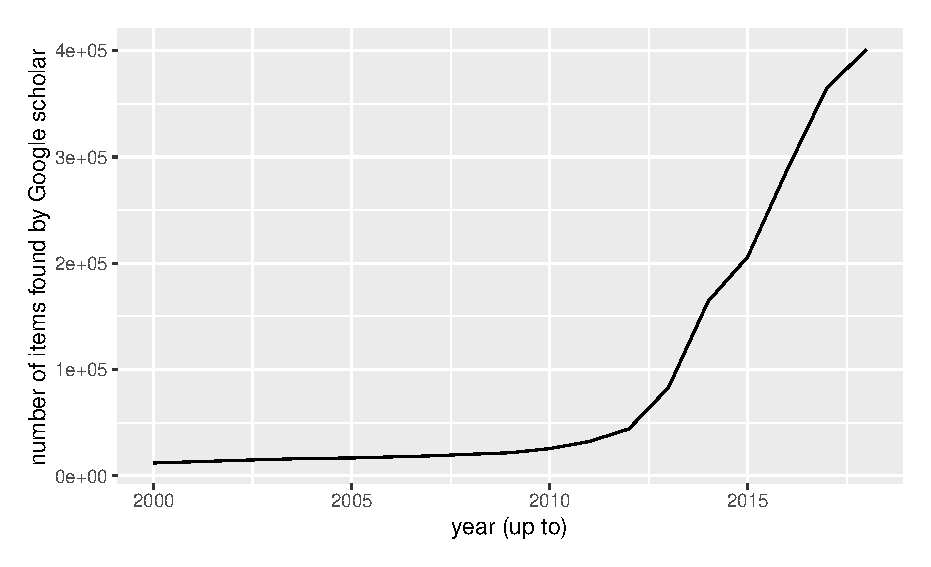
\includegraphics[width=\textwidth]{bigdata.eps}
\caption{Number of items found by Google scholar when searching the exact phrase \emph{big data} up to different years.} 
\label{fig_bigdata}
\end{figure} 



There are several issues related to large datasets, including: how to store them, how to load them, and how to analyze them. Our interest in this thesis is in the last one. Although the last issue, the same as the two others could be solved to some extent by increasing the computation power of the hardware we use, we believe statistical methods and ideas can provide solutions that are easy to understand, capable of being implemented in different situations, accurate, and also mathematically sound. This becomes more important when we realize increasing the computation power and size of available datasets are highly and positively correlated. 



In Table \ref{tab_comptime1} we compare the computation time when the sample sizes $n=10, 10^2, 10^3, 10^4, 10^5, 10^6, 10^7$, for some simple computational tasks including:

\begin{itemize}
\item Generating a random sample from standard normal of size $n$.
\item Finding the mean of the generated sample.
\item Finding the variance of the generated sample.
\item Fitting a linear model to the generated sample as the predictor and $y = 1 + 3x + \epsilon$, where $\epsilon\sim N(0, 0.01)$.
\item Fitting a MAD (mean absolute deviation) regression to the same data.
\end{itemize}



\begin{table}[ht]
\centering
\begin{tabular}{lccccc}
  \hline
Sample size & Generation & Mean & Variance & LS & MAD \\ 
  \hline
 $10$ & 0.00 & 0.00 & 0.00 & 0.00 & 0.00 \\ 
 $10^2$ & 0.00 & 0.00 & 0.00 & 0.00 & 0.00 \\ 
 $10^3$ & 0.00 & 0.00 & 0.00 & 0.00 & 0.00 \\ 
 $10^4$ & 0.00 & 0.00 & 0.00 & 0.00 & 0.06 \\ 
 $10^5$ & 0.00 & 0.00 & 0.00 & 0.01 & 3.75 \\ 
 $10^6$ & 0.08 & 0.01 & 0.00 & 0.32 & 764.37 \\ 
 $10^7$ & 1.05 & 0.01 & 0.06 & 3.46 & 60558.83 \\ 
   \hline
\end{tabular}
\caption{Computation time (in seconds) of different methods for different sample sizes.} 
\label{tab_comptime1}
\end{table}



As we may see, for some analyses, the computation time increases linearly as the sample size increases, but for others, it would even speeds down with a sub-linear rate. Once the cause of expensive computation time is the sample size, an effective solution could be to split the very large sample into smaller sub-samples and then analyze them separately. As each sub-sample has a smaller size, and analyzing these different sub-samples are independent of each other (can be run in parallel), the overall computation time can be decreased. 

Splitting a sample into smaller chunks, then analyzing each part separately, and finally combine the results of these analyses is a known methodology to deal with large samples. Some authors have called this \emph{Software Alchemy}, \cite{matloff2014}. This idea is also at the heart of MapReduce methodology \citep{dean2008}. The split-apply-combine strategy in the R packages {\tt{plyr}} and {\tt{dplyr}} also uses this idea \citep{wickham2011}. All these would show the importance and effectiveness of this approach. 


However, most of these implementations would consider independent sub-samples, or non-clustered data. Our goal in this thesis is to extend the existing methodology to the cases where the subjects would form clusters of correlated data. This type of data is very common in medical studies in particular, but they also can be observed in any longitudinal or multilevel study. Some examples of such data are measurement on offsprings of the same animal, data collected from family members, data collected from different countries in a meta-analytic setting, measuring body temperature of the same person several times, ratings of the same book by different people, measuring hearing ability of elderly people for several frequencies, measuring primary vital signs (body temperature, heart rate, respiratory rate, and blood pressure) for each person, etc.

As we have seen in Table~\ref{tab_comptime1}, even for non-clustered data and simple models, increasing the sample size could cause very expensive computation times. The time needed to fit a MAD regression with one predictor to a sample of size 10 million is around 18 hours. Now, if we have clustered data that demands more complicated models to account for correlations, things would get even more difficult. In case of clustered data, the sample size can be seen from different points of view. 





\section{Large clustered data}

Consider a study which measures (at most) $m$ outcomes for $N$ clusters, each $n_i$ times. Let $y_{rij}$ be the $j$th measurement taken on the $i$th cluster for the $r$th outcome, $i=1,\ldots,N$, $r=1,\ldots,m$ and $j=1,\ldots,n_{ri}$. As a simple example, take $m=4$ responses as the vital signs: body temperature, heart rate, respiratory rate, and blood pressure, measured for $n_1 = n_2 = n_3 = n_4 = 100$ hospitalized patients. And assume these measurements are done every $4$ hours. For example, $y_{111}$ is the body temperature of the first patient measured for the first time. 

A general scheme of such clustered data is presented in Figure~\ref{fig_scheme}. A suitable model for such data should appropriately respect the correlation structures imposed by the fact that several measurements are done on the same subject. While even for moderate sample sizes, fitting such models could already become challenging, we may face a greater challenge when the size of dataset makes it eligible for the title \emph{big data}. 

\begin{figure}
\centering
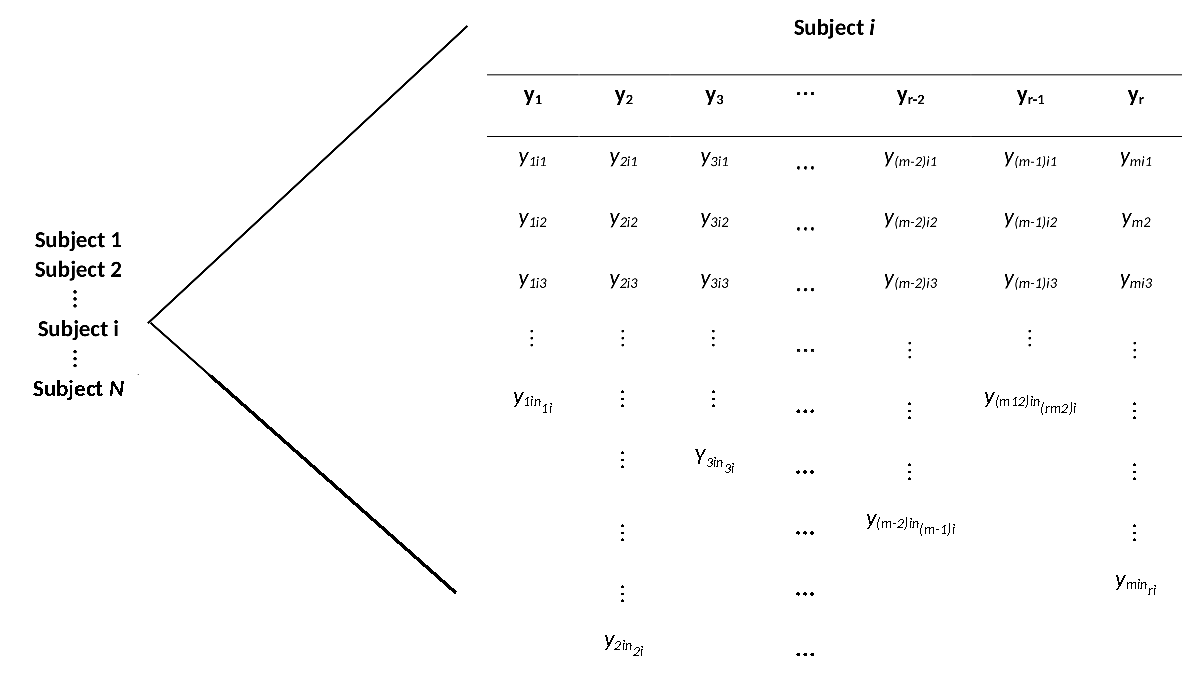
\includegraphics[width=\textwidth]{scheme_new.eps}
\caption{General scheme of the clustered data we consider through this thesis.} 
\label{fig_scheme}
\end{figure} 


As it was mentioned, for non-clustered data big would mean a large number of subjects. However, in our case, a dataset could be entitled as \emph{big data} in different situations. In case of the clustered data of interest in this thesis, data are considered to be big if at least one of the following applies:
\begin{itemize}
\item When the sample size, $N$, becomes very large,
\item When the cluster sizes become very large:
\begin{itemize}
\item When the number of measurements per outcome for some clusters, $n_{ri}$'s, becomes very large,
\item When the number of outcomes, $m$, becomes very large.
\end{itemize}
\end{itemize}

Note that, \emph{big} would be different for $N$, $n_{ri}$, and $m$. For example, in case of a MAD regression, we have seen a dataset of size $N=100,000$ could be analyzed in $0.001$h, increasing the sample size to $N = 1000,000$ would increase the computation time to $0.2$h, which is not fast, but still feasible, but $N=10,000,000$ would take around $17$ hours which could be too much. Therefore, in the case of a simple MAD regression, we may consider $N>10,000,000$ as \emph{big}.

When it comes to clustered data, however, a different story is going on. Some 100's could already be big in case of cluster size, $n_{ri}$ (see Amazon book ratings data in Section~\ref{mot_amazon}), and even some 10's is \emph{big} when we consider the number of outcomes $m$ (see Hearing data in Section~\ref{mot_hearing}).

It goes without saying that, in reality, any combination of the above situations could happen. Our aim in this thesis is to provide appropriate methodology to: 1- split the data into smaller chunks, 2- analyze each split, 3- combine these analyses in an efficient way. Our methodology should consider the nature of the data. While the mere task of splitting would already breaks down the difficult (sometimes infeasible) problem into smaller easier and feasible to analyze pieces, sometimes the structure of the data would allow for some \emph{smart} other than random splitting which would then provide more gain. Our aim in this thesis is to cover all of the situations which a dataset of clustered subjects could be called \emph{big}. 

In developing these methodologies we will make sure to keep two promises:

\begin{itemize}
\item While each methodology can deal with one situation, it should be easily possible to combine methodologies to deal with a combined situation.

\item The splitting and combining steps of our methodology should be as independent as possible from the analyses step, so one can easily (or with a minor modification) use it for its desired analysis.
 
\end{itemize}

\section{Data splitting: a unified approach}

Data splitting is a general idea to deal with big, massive, and large data. Large here could be any of the cases we have mentioned above, or a combination of them. Our general approach to deal with this situation consists of three main steps as follows. We call these three steps \textit{data splitting}.

\begin{enumerate}
\item \textbf{Splitting}: in this step, the data should be splitted into smaller chunks in a way that analyzing each of them becomes more convenient that the dataset as a whole. This convenience would at least come from having sub-samples of smaller sizes, but it could be possible to perform the splitting in a way that some other nice features (balancedness, for example) that the original data does not own, can be created in all or some of these sub-samples.

\item \textbf{Analyzing}: in this step, each split of data will be analyzed using the conventional methods. Therefore, using \emph{data splitting} approach, one can use its own favorite methodologies which are only suitable for small to moderate sample sizes. Typically, with \emph{data splitting} approach, the only information one needs to extract and keep from analyzing each split of data are: the estimated parameter vector, and their covariance matrix (if there is a need to provide standard errors of such estimates).

\item \textbf{Combining}: within this unified framework, each parameter in the model could be estimated several times. As our interest is to have one single set of parameter estimates, the last step in this paradigm is to combine all of analysis results from the second step into one single set. This should be done via appropriate combination rules. The combination rule is simply a weighted average of the results from different splits. Therefore, there is the need for proposing appropriate weights. Also, when it comes to combine covariance matrices, the fact that these results are coming from different (possibly dependent) sub-samples should be well respected. 

\end{enumerate}



In the following sections we will review different splitting approaches, also their appropriate combination rules. We will also give examples of our motivating datasets where each of these approaches could be beneficial. 

\section{Different types of splitting}

We have already discussed the MapReduce, or split-apply-combine approaches. The main splitting technique that is implemented using such approaches is to split the data: 1- randomly, 2- at subject level. Throughout this thesis we would call the splitting at the subject level \emph{horizontal splitting}. The reason for that can be seen in the Figure~\ref{fig_scheme}. If we illustrate the splits by separating lines, such lines will be horizontal. On the other hand, if the splitting is done for the data within a subject, then the lines should be drawn vertically. This case is specific to the clustered data where we have more than one observation for each subject. 

While random splitting (assigning members of each split at random) is an effective way in many situations, there are cases where assigning members of each split based on a predefined structure has an added value. We call such splitting approach structural splitting as opposed to random splitting. In the following we will give an overview of the four types of splitting (combinations of random/structured and horizontal/vertical splitting), and present examples where each of them could be useful. We will also briefly go over analyzing and combining steps.

\subsection{Random horizontal splitting}    

Random horizontal splitting, as its name suggests, tries to assign different subjects to different splits at random. There are several ways to do this task, the way we have used in our implementations is as follows. For a sample of size $N$,

\begin{enumerate}
\item To split the dataset into $M$ sub-samples, take $m = \floor{N/M}$ as the size of each split to make sub-samples of roughly the same sizes.
\item Generate a random sample of size $N$ from standard normal.
\item Order the generated sample.
\item Divide the ordered indexes into (M-1) parts of size $m$, and the $m$th chunk will include all the remaining indexes. These will be the index of subjects that should be assigned to each split.
\end{enumerate}

Note that, $M$ should be carefully selected. Two main points to consider when selecting $M$ are first to make sure the resulting sub-samples are small enough to keep the computation time at an acceptable level, but at the same time one needs to be careful that the sub-samples stay large enough, so the methodologies can still be applied on them in a valid way.

Assume $\widehat{\theta}_1, \ldots, \widehat{\theta}_M$ are the estimated parameters from $M$ sub-samples, the data splitting estimate of this parameter can be computed as follows:

\begin{equation}
\label{eq_estimate}
\widetilde{\theta} = \sum_{m=1}^M w_m\widehat{\theta_m},
\end{equation}
where $w_m$'s are the combination weights, and $\sum_{m=1}^M w_m = 1$. An appropriate set of weights could be assigned proportional to the size of each split, i.e., a larger split contributes more to the final estimate. We would call such weights proportional weights in this thesis:

\begin{equation}
\label{eq_prop_w} 
w_{prop, i} = \frac{m_i}{N}.
\end{equation}

Of course, in case of random splitting, as the split sizes are roughly the same, one can simply assign equal weights to different sub-samples. Such weights are called equal weights in this thesis:

\begin{equation}
\label{eq_equal_w}
w_{equal,i} = \frac{1}{M}.
\end{equation}

The combination rule in case of horizontal splitting is simpler than vertical splitting. This comes from the fact that the sub-samples are independent in this case, therefore, one does not need to be concerned about the correlations between the estimates coming from different sub-samples. For a general weight $w_i$, consider $\mathrm{Var}(\widehat{\theta}_i) = \sigma^2_i$, then the variance of data splitting estimator can be computed as follows:

\begin{equation}
\label{eq_variance1}
\mathrm{Var}_{horizontal}(\widetilde{\theta}) = \sum_{m=1}^M w_m^2 \sigma_m^2.
\end{equation}

As having a smaller variance is a desired property for an estimator, Equation (\ref{eq_variance1}) would give an idea about an alternative way of assigning weights to our estimates: the weights should be computed in a way that the variance in (\ref{eq_variance1}) becomes minimized. In this thesis, such weights are called optimal weights. We define the optimal weights as the minimizer of the following objective function:

\begin{equation}
\label{eq_objective_opt_w}
Q = \sum_{m=1}^M w_m^2 \sigma_m^2 - \lambda \left(\sum_{m=1}^M w_m -1 \right),
\end{equation}

where $\lambda$ is a Largange multiplier to make sure that the sum of estimated optimal weights is still 1. Solving the optimization problem in (\ref{eq_objective_opt_w}) would lead to the following optimal weights,

\begin{equation}
\label{eq_opt_w}
w_{opt, i} = \frac{1/\sigma^2_i}{\sum_{m=1}^M 1/\sigma^2_m},
\end{equation}

As one may see, a larger weight is given to a sub-sample with a smaller variance.


In using optimal weights, one needs to be concerned about the fact that, optimal weights are including parameters from model, which then needs to be replaced by an estimate (we will discuss different ways of doing it in the coming chapters), and these estimates will come with their own variability. So, if the variability these estimates will bring together with them becomes larger than the variability that the optimal weights could decrease, then it is better to use the simpler parameter-free weights.

An example in our motivation datasets that random horizontal splitting can be beneficial is the Divorce in Flanders dataset, where clusters are formed by family members. While each family is at most of size 7, the number of total available families is large enough to make conventional software to fail. By splitting this large sample randomly and at the family level (horizontally), we could be able to fit the models and answer the research questions.

\subsection{Structured horizontal splitting}

As we have discussed, random horizontal splitting has been used by many researchers in different contexts to deal with big data issue. However, a randomly horizontal split would only decrease the sample size. So all of our gain is due to having smaller sample sizes. We have observed that they are cases where splitting using a pre-defined structure would provide some added benefits on top of just having smaller sub-samples.

It is a well-known fact that a balanced study deign works better than an unbalanced one. By balanced we mean, the number of available data for each cluster is the same. In fact, most of the studies are planned to be balanced, but in practice they would rarely end up like that. One can see several reasons for that, for example, the required materials are not enough, some patients die, some animals fail to follow the instructions, etc. Therefore, while having a balanced set of data is desired and even planned, we will usually have an unbalanced data to analyze. 

Although most of the data in practice are unbalanced, one can usually find balanced sub-sets of those data. Take our example on a developmental toxicity study. There, the clusters are made of fetuses within litters. Obviously, different mothers would have different number of babies: an inevitably happened unbalanced data. However, it is not like that the number of fetuses within litter from every single mother is different from the others. Table \ref{tab_litter_size} shows unique number of fetuses in different litters with their frequencies. As one may see, we have a limited number of cluster sizes. Therefore, although the complete data is unbalanced, it is formed by balanced sub-sets. An structured horizontal splitting would assign all clusters of the same size to one sub-sample. 


\begin{table}[ht]
\centering
\label{tab_litter_size}
\caption{Unique cluster sizes and their frequency in a developmental toxicity case study for the response DEHP.}
\begin{tabular}{lcccccccccccc}

  \hline
Cluster size & 9 & 10 & 15 & 8 & 12 & 13 & 14 & 6 & 7 & 3 & 11 & 16 \\ 
  Frequency & 10 & 9 & 3 & 12 & 20 & 18 & 6 & 4 & 5 & 4 & 9 & 4 \\ 
   \hline
\end{tabular}
\end{table}

As it was mentioned, there are several benefits for a balanced dataset, and in the special case of clustered data, we have shown that a closed-form solution exists when the cluster sizes are balanced, whereas for unbalanced data one needs to fit the models using iterative procedures. For very large datasets, the iterative procedures could be prohibitive and slow. While, a closed-form solution can be computed much faster. We have observed tens of thousands time faster computation using structured horizontal splitting based on the cluster sizes. Two cases are studied in details: clustered data with a compound-symmetry (CS) covariance structure, and clustered data with an autoregressive of order 1 (AR1) covariance structure. It worth to note that, even if the closed-form does not exist, with a balanced dataset one would have a faster and more stable convergence compared to unbalanced data.

The two considered covariance structures would cover a wide range of applications: where the correlation between to  members of a cluster is always the same (compound-symmetry), and when it decreases when the distance between the two observations becomes larger (AR1). For these two cases, the existance of the closed-form solution are shown using sufficient complete statistics. Then these closed-form solutions are obtained, also various kinds of weights, including optimal weights are computed for each case. On top of the already discussed weights, as we have clusters of all different sizes in each sub-sample here, we have proposed another type of weights, as follows,

\begin{equation}
\label{eq_size_prop_w}
w_{size-prop, i} = \frac{m_i n_i}{\sum_{k=1}^ M m_k n_k},
\end{equation}

In some cases that the cluster size is also important (other than the number of subjects in each sub-sample), such weights would perform better. We have shown that AR(1) is one of these cases, while for the CS, proportional weights would work fine. 

Note that, the structured horizontal splitting idea is very general and all the introduced methodologies regarding different weights, combination rules, etc., can be used for any suitable structure of splitting (as long as they are horizontal), but in this thesis we only consider the cases where the structure is defined based on size of the clusters. 

\subsection{Random vertical splitting}

The horizontal splitting techniques that we have introduced and discussed so far would be beneficial when the number of clusters ($N$) is large, but the cluster size is still small or moderate, so by breaking down the large $N$ into $M$ smaller sub-samples, we can manage to solve our problem. But there are examples where the size of some or all of the clusters is also very large. And as we have mentioned, large for a cluster size has a much smaller magnitude compared with large for the number of clusters. In such cases, horizontal splitting would not help much, because each cluster in our sub-samples is still large, so by horizontal splitting we just breakdown one problem into $M$ problems. 

As n example, take the Amazon book ratings. There, we have the ratings for many books given by different buyers. Therefore, each book could possibly be rated by thousands of people. This will for very large clusters where even the simple models would fail to converge. In such a case, horizontal splitting cannot solve our problem. To solve the issue here, we have to perform the splitting within the subject. For example, if there are 5000 people rating a book, in order to make smaller clusters in our sub-samples, we have to split these 5000 people, e.g., into 100 sub-samples, each of size 50. 

As long as the interest is in the parameter estimate, the combination rules in (\ref{eq_estimate}) is still valid. But the difficulty will appear in deriving the combination rule for the variances. As the data from different clusters are shared among different sub-samples, in other words, one cluster is present in more than one sub-sample, the estimated parameters from different sub-samples are correlated, and obviously, when combining the variances, these correlations should be taken into account. 

One way to deal with the combination rule of variance in case of vertical splitting is to look at our sample splitting based model fitting in the pseudo-likelihood methodology, rather than the likelihood. In fact, once the dataset is analyzed in whole we use the conventional likelihood theory by finding the estimate of our parameters by maximizing the likelihood function. But when the data is splitted into some sub-samples, each of these sub-samples are analyzed using a likelihood theory, but their combination is not the original likelihood function anymore. It is called pseudo-likelihood. Roughly speaking, pseudo-likelihood theory tries to replace the complex or difficult likelihood function with something simpler or easier. But maximizing both likelihood or pseudo-likelihood functions would follow the same goal, i.e., estimate the same set of parameters, but with different precision.

From Cram\'{e}r-Rao's lower bound we know that the lower bound for variance can be achieved by a maximum likelihood estimator. In other words, any other estimator (including maximum pseudo-likelihood) would come with a variance larger than the one from a maximum likelihood. Therefore, having the easier problem to solve comes at the price of losing a bit of accuracy. 

Let us define the pseudo-likelihood in plain English. Assume we have a sample $\mathbf{y}$ and using that we want to estimate the parameters vector $\theta$ via the log-likelihood function $\ell(\theta; \mathbf{y}$. Via sample splitting, we split the sample $\mathbf{y}$ into $M$ sub-samples $\mathbf{y_1}, \ldots, \mathbf{y_M}$, then feed them to the same likelihood function and estimate the parameter vector $\theta$ $M$ times. Under pseudo-likelihood paradigm, one can look at this as estimating a parameter vector $\Theta = (\theta_1, \theta_2, \ldots_3, \theta_M)$ using the sample $\mathbf{Y} = (\mathbf{y_1}, \ldots, \mathbf{y_M})$ via maximizing the pseudo-likelihood function $p\ell(\Theta, \mathbf{Y})$. Note that, $\theta_1 = \theta_2 = \theta_3 = \ldots = \theta_M$. 

Now that the problem is defined under a pseudo-likelihood theory, all the results obtained there can be carried over to the data splitting as well. If we consider matrix $A$ that combines the estimates, i.e., $\widetilde{\theta} = A\widehat{\Theta}$, then the most important result we can present is:

\begin{equation}
\label{eq_clt_pseudolikelihood}
\sqrt{N}(\widehat{\theta} - \theta) = \sqrt{N}(A\widehat{\Theta} - A\Theta) \stackrel{d}{\sim} N\left(\mathbf{0}, A I_0^{-1} I_1 I_0^{-1} A^{T}\right),
\end{equation}

where $T$ means the transpose, and $I_0$ and $I_1$ are defined as follows,
\begin{equation}
\label{eq_hessian_gradient_pl}
I_0(\Theta) = \mathrm{E} \left(\frac{\partial^2 p\ell(\Theta; \mathbf{Y})}{\partial \Theta^T \partial \Theta} \right),\; I_1(\Theta) = \left[\left(\frac{\partial p\ell(\Theta)}{\partial \theta} \right)^T \frac{\partial p\ell(\Theta)}{\partial \theta}  \right].
\end{equation}

More details on pseudo-likelihood interpretation of the data splitting can be found in \cite{Iddi2011}. However, a main difficulty to find the variance in (\ref{eq_clt_pseudolikelihood}) if the need to cluster-wise hessian and gradient of the pseudo-likelihood function. This could easily become expensive. Another difficulty with this approach comes from the fact that, depending on the derivative and hessian means this variance estimator needs to computed case by case. For example, the results obtained for a logistic regression cannot used for another model without the necessary modification. To overcome these difficulties, we have considered an alternative solution proposed by \cite{hoffman2001} in different context. Their approach is called within cluster re-sampling, which was later on extended and renamed to \emph{multiple outputation} by \cite{follmann2003}.

In order to explain the motivation behind the multiple outputation technique, consider clustered data where the cluster consists of blood pressure of a patient visiting a hospital several times. The objective of the study is the severity of a disease which is highly correlated with blood pressure (more severe the disease, the larger the blood pressure). As the blood pressure is measured every time the patient is visiting the hospital, a larger cluster size, means the patient has visited the hospital more, which itself means the patient had more issues with the blood pressure, so a more severe state of the disease. In other words, in such situations the size of the cluster is also correlated with the response and objective of the study. Such situations are also called \emph{informative cluster size} in the literature. The correlation of cluster size and the response should be respected in the model, otherwise it could cause issues. Multiple outputation has been proposed to deal with this problem.

Within cluster resampling proposed by \cite{hoffman2001} to deal with the so-called informative cluster size, when it is a nuisance parameters, i.e., we are not interested to study the correlation of the response and cluster size, we just want estimates of other parameters which are not affected by this correlation. \cite{hoffman2001} proposed to take sub-samples of size 1 from each cluster repeatedly to form a sample on non-clustered data every time. Then the conventional methods can be used for each of these non-clustered data. The results then can be combined via combination rules which are similar to (\ref{eq_estimate}) for the estimates. But for the variance \cite{hoffman2001} proposed the following combination rule:

\begin{equation}
\label{eq_combination_variance}
\mathrm{Var}(\widetilde{\theta}) = W - \left(1 + \frac{1}{M}\right) B,
\end{equation}
where $W$ and $B$ are within and between sub-samples variances respectively. These quantities are defined as follows,
\begin{equation}
\label{eq_W_B_Var}
W = \frac{1}{M} \sum_{i=1}^M \sigma^2_m,\; B = \frac{1}{M-1} \sum_{i=1}^M \left(\widehat{\theta}_i - \widetilde{\theta} \right)^2.
\end{equation}

As one may see, the combination rule for the variance in (\ref{eq_combination_variance}) is also intuitively interesting also. It states, the variance of the data splitting estimator is an average of the variance in different sub-samples, but when we subtract it from the sample variance of estimated parameter from different sub-samples. Looking at this combination rule, one might also understand the reason behind naming this method multiple outputation by \cite{follmann2003}. That comes with various similarities of this technique with multiple imputation. Although, the similarities are technically rather than literally. 

First let us say a word on multiple imputation itself. Multiple imputation (MI) is an effective way to deal with missing data issue. The traditional missingness remedies would try to either ignore that missing part of the sample, or replace it with a single plausible value. This way, one would treat a missing before and now imputed value the same as a value which is originally observed. In order to respect the fact that imputed values are actually imputed and as well could be any other value, \cite{rubin1978} proposed to replace each missing value with several values and not just one single value. 


Now we may look at similarities of MI and MO. As it was mentioned, multiple imputation creates artificial data and augment it to the incomplete sample to make it complete, on the contrary, but in a similar way, multiple outputation would every time put some part of the same out of the analysis. Therefore, multiple \textbf{im}putation increases the sample size by including new artificial data, while multiple \textbf{out}putation decreases the sample size by selecting only a subset of them. But in both of the methods, we will have several datasets to analyze rather than the one single original dataset. So, in both methods we estimate each parameter several times. This is also reflected in the variance estimator. Let us remind the combination rule for variance from \cite{rubin1987},

\begin{equation}
\label{eq_comb_var_MI}
\mathrm{Var}(\widehat{\theta}_{MI}) = W + (1 + \frac{1}{M}) B.
\end{equation}

As one may see, the only difference of (\ref{eq_comb_var_MI}) and (\ref{eq_combination_variance}) is in the fact that MI would add the between datasets variability of the estimated parameter to the averaged variance, while MO would subtract this. And intuitively, that would also make sense, in case of MI we artificially increase the sample size, so we would get a smaller variance which needs a correction (to become larger, as it should be), but in case of MO we decrease the sample size, so a larger variance would be obtained, which is the also corrected in the same was as MI just with a different sign.

Because of the discussed similarity and for the vast use of multiple imputation in practice, we have developed part of contributions with the target to be used in data splitting for the case of multiple imputation. As for many cases, the conclusions and results from MI are also valid for MO, and vice versa. 

We have extended the idea in within cluster re-sampling and multiple outputation to it them suitable for our purpose: analyzing clustered data with big clusters. The so-called iterative multiple outputation (IMO) procedure is proposed to fulfil this role. IMO is proposed as follows,

\begin{enumerate}
\item \textbf{Start.} Select an initial number of sub-samples, $M_0$, and sub-sampling size $m$. Take $M_0$ sub-samples of size $m$, fit the model to each and obtain $\widehat{\theta}_i$ and its variance $\Sigma_{\widehat{\theta}_i}$ ($i=1,\ldots,M_0$). Then compute 
\begin{equation}
\label{intro_comb_rules}
\widetilde{\bftheta}_{M_0} = \sum_{i=1}^{M_0} \widehat{\bftheta}_i,\;\; \Sigma_{\widetilde{\theta_{M_0}}}=\widehat{W}_{M_0} - \left( \frac{M_0+1}{M_0} \right) \widehat{B}_{M_0}.
\end{equation}

			\item \textbf{Update.} For $m>M_0$, \begin{equation}
	\label{introupdate}
	\widetilde{{\bftheta}}_{m+1}=\frac{m\widetilde{\bftheta}_m + \widehat{\bftheta}_{m+1}}{m+1},\; \Sigma_{\widetilde{\theta}_{m+1}}=\widehat{W}_{m+1} - \left( \frac{m+1}{m} \right) \widehat{B}_{m+1}.
	\end{equation}
	\item \textbf{Distance.} Compute: $d_{m+1}=d(\widetilde{\bftheta}_{m+1},\widetilde{\bftheta}_{m})$ using an appropriate distance.
	\item \textbf{Stopping rule.} $d_{j} < \varepsilon$ for $j=m+1,\ldots,m+k_0$.
\end{enumerate}
Where for $m=r$ we have,
\begin{equation}
\widehat{W}_r= \frac{\sum_{i=1}^r \sigma_{\widehat{\theta}_i}}{r},\; \widehat{B}_r= \frac{\sum_{i=1}^r (\widehat{\theta}_i - \widetilde{\theta}_r)(\widehat{\theta}_i - \widetilde{\theta}_r)'}{r-1}.
\end{equation}

We may remark that, there are cases only $M=1$ sub-sample would be sufficient to obtain results almost as efficient as analyzing the full dataset. We have studies this matter in detail and called such estimators \textit{finite information limit estimators}. We have also proposed procedures to detect this property.

A very useful dataset to illustrate the usefulness of random vertical splitting is the Amazon's book ratings dataset. This set of data consists of ratings of several books (from 1 to 5) on Amazon website. Each book is rated by different number of people, which could be as small as 1 and as large as 20,000. So we will deal with clustered data of very variable and large sizes. 


\subsection{Structured vertical splitting} 

So far we have discussed random horizontal and random vertical splitting, as well as structured horizontal splitting. In case of the vertical splitting also, pre-defining some structures to take the sub-samples other thank taking them just at random could be beneficial. We have already seen one application of structured splitting in case of horizontal splitting, which enabled us to form balanced sub-samples. Defining an structure is not always for computation efficiency. Sometimes, without such structure, estimating the model parameters is not possible. 

We have considered an important case of jointly modeling several outcomes via random effects as a useful example for structured vertical splitting. Such a problem can easily become infeasible when the number of outcomes becomes large (even tens of them). \cite{fieuws2006, fieuws2007} proposed to analyze all possible pairs of all outcomes instead of analyzing them simultaneously. Then use appropriate combination rules to find the parameters of the model of interest. To illustrate the problem, also to show how structural vertical splitting is similar to the approach of \cite{fieuws2006, fieuws2007}. Also, to see how it is different from random vertical splitting, we present a simple example. 

Imagine we have 3 outcomes to be jointly modeled. A random effects approach would fit a separate model to each outcome, then let them to be correlated by defining a joint distribution for their random effects. This joint distribution is usually a normal distribution where its covariance matrix would capture the dependencies between different outcomes. Let us elaborate more here, if the three separate models (all linear) for the three outcomes are defined using the following general form:

\begin{equation}
\label{eq_SV_models}
\begin{cases}
y_{1ij} = \beta_1 + b_{1i} + \epsilon_{1ij} \\
y_{2ij} = \beta_2 + b_{2i} + \epsilon_{2ij} \\
y_{3ij} = \beta_3 + b_{3i} + \epsilon_{3ij},
\end{cases}
\end{equation}
we let the three random intercepts to be normally distributed as follows,
\begin{equation}
\label{eq_SV_D}
\begin{bmatrix}
b_{1i} \\
b_{2i}\\
b_{3i}\\
\end{bmatrix} \sim N \left ( 
\begin{bmatrix}
0 \\
0\\
0\\
\end{bmatrix}, 
D=\begin{bmatrix}
D_{11} & D_{12} & D_{13}\\
 & D_{22} & D_{23}\\
&& D_{33}\\
\end{bmatrix}
\right).
\end{equation}
Therefore, the parameter of interest, $\bftheta$, is as follows:
\begin{equation}
\label{eq_SV_theta}
\bftheta= (\beta_1,\beta_2,\beta_3, D_{11},D_{22},D_{33},D_{12}, D_{13}, D_{23}).
\end{equation}
As we have $3$ outcomes, the number of pairs will be $M=3\times (3-1) /2 =3$. However, unlike random vertical splitting where usually all parameters of interest are estimated in each sub-sample, here, because of the special structure we have imposed on the sub-samples, each of them would estimate part of parameter vector. The parameters estimated in each pair ($\bftheta^{(s)}$) are as follows:
\begin{equation}
\label{eq_SV_pairs}
\begin{cases}
\bftheta^{(1)}=\theta_{(y_{1ij},y_{2ij})} = (\beta_{1_1},\beta_{2_1},D_{11_1},
,D_{22_1},D_{12_1}) \\
\bftheta^{(2)}=\theta_{(y_{1ij},y_{3ij})} = (\beta_{1_2},\beta_{3_2},D_{11_2},
,D_{33_2},D_{13_2}) \\
\bftheta^{(3)}=\theta_{(y_{2ij},y_{3ij})} = (\beta_{2_3},\beta_{3_3},D_{22_3},
,D_{33_3},D_{23_3}),
\end{cases}
\end{equation}
as one may see in (\ref{eq_SV_pairs}), each $\bftheta^{(s)}$ ($s=1,2,3)$ is a subset of $\bftheta$ in (\ref{eq_SV_theta}. Now, the stacked vector combining all parameters estimated in different sub-samples $\boldsymbol{\Theta}'=(\bftheta^{(1)},\bftheta^{(2)},\bftheta^{(3)})$ can be constructed as follows:
\begin{multline}
\label{eq_SV_Theta}
\boldsymbol{\Theta}'=(\beta_{1_1},\beta_{2_1},D_{11_1},
,D_{22_1},D_{12_1}, \beta_{1_2},\beta_{3_2},D_{11_2},
,D_{33_2},D_{13_2},\beta_{2_3},\beta_{3_3},\\ D_{22_3},
,D_{33_3},D_{23_3}).
\end{multline}
As one may see, the covariance parameters ($D_{12},D_{13}, D_{23}$) are only estimated once using their corresponding pair, but the rest of parameters are appearing in two out of three pairs. Therefore, to combine these estimates we cannot just average all estimates as we did in (\ref{eq_estimate}). The weight matrix to perform the appropriate combination can be defined as follows,
\vspace*{2mm}

\renewcommand{\kbldelim}{(}% Left delimiter
\renewcommand{\kbrdelim}{)}% Right delimiter

\[
 \resizebox{\textwidth}{!}{  
  A = \kbordermatrix{
    & \beta_{1_1}&\beta_{2_1}&D_{11_1}
	&D_{22_1}&D_{12_1}& \beta_{1_2}&\beta_{3_2}&D_{11_2}
	&D_{33_2}&D_{13_2}&\beta_{2_3}&\beta_{3_3}&D_{22_3}
	&D_{33_3}&D_{23_3} \\
\beta_1 & 1 & 0 & 0 & 0 & 0 & 1 & 0 & 0 & 0 & 0 & 0 & 0 & 0 & 0 & 0 \\ 
  \beta_2 & 0 & 1 & 0 & 0 & 0 & 0 & 0 & 0 & 0 & 0 & 1 & 0 & 0 & 0 & 0 \\ 
  \beta_3 & 0 & 0 & 0 & 0 & 0 & 0 & 1 & 0 & 0 & 0 & 0 & 1 & 0 & 0 & 0 \\ 
  D_{11} & 0 & 0 & 1 & 0 & 0 & 0 & 0 & 1 & 0 & 0 & 0 & 0 & 0 & 0 & 0 \\ 
  D_{22} & 0 & 0 & 0 & 1 & 0 & 0 & 0 & 0 & 0 & 0 & 0 & 0 & 1 & 0 & 0 \\ 
  D_{33} & 0 & 0 & 0 & 0 & 0 & 0 & 0 & 0 & 1 & 0 & 0 & 0 & 0 & 1 & 0 \\ 
  D_{12} & 0 & 0 & 0 & 0 & 1 & 0 & 0 & 0 & 0 & 0 & 0 & 0 & 0 & 0 & 0 \\ 
  D_{13} & 0 & 0 & 0 & 0 & 0 & 0 & 0 & 0 & 0 & 1 & 0 & 0 & 0 & 0 & 0 \\ 
  D_{23} & 0 & 0 & 0 & 0 & 0 & 0 & 0 & 0 & 0 & 0 & 0 & 0 & 0 & 0 & 1 
  }
}
\] 


\vspace*{2mm}
\noindent Obviously, $\sum_i A_i$ (with $A_i$ the $i$th row of $A$) shows the number of times each parameter is estimated. Therefore, by defining $W$ with each of its rows computed as $A_i / \sum_i A_i$, and pre-multiplying it by $\widehat{\boldsymbol{\Theta}}$ would provide the appropriate averaging. The same goes for the variance combination rule. \cite{fieuws2006, fieuws2007} used a pseuo-likelihood approach to find the combined covariance matrix (the same as in \ref{eq_clt_pseudolikelihood}), we could show using \ref{eq_combination_variance} with appropriate weights works the same, but much faster.

As one may see, only the covariance matrix of the random effects have $6$ parameters to be estimated, if one decides to add random slopes also, then the number of parameters will increase to $(6\times7)/2 = 21$. Once the number of responses becomes slightly large, the number of parameters will dramatically increase. This would face all conventional methods with serious problems, and the problem can be unfeasible. Figure \ref{fig_strucVert} shows how the number of parameters only in the covariance matrix of random effects would increase when the number of responses increases. As we may see in this figure, even for less than 100 responses, the number of parameters becomes extremely large.

\begin{figure}
\centering
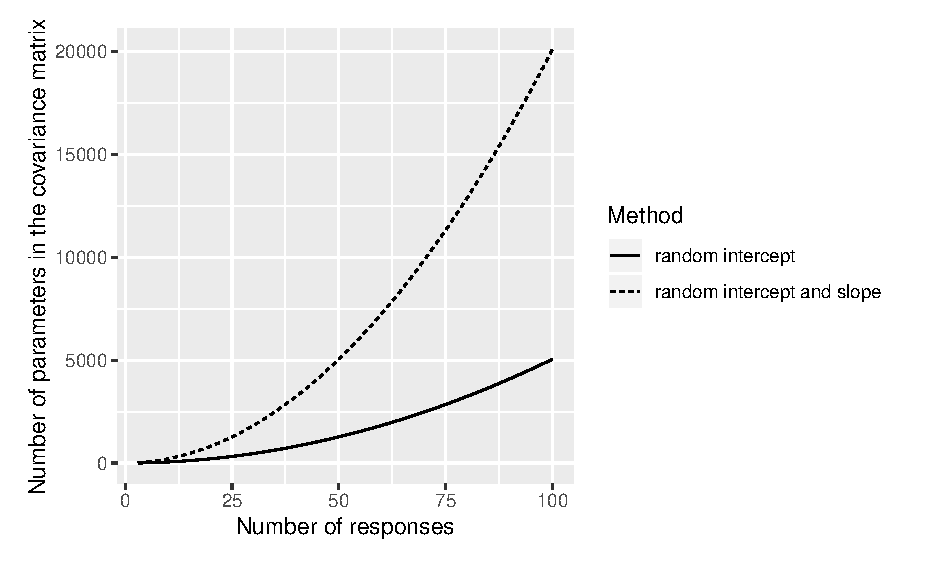
\includegraphics[width=\textwidth]{strucVert.eps}
\caption{Number of parameters in the covariance matrix of jointly normally distributed random effects for different number of responses using only random intercept or random intercept and slope models.} 
\label{fig_strucVert}
\end{figure} 

Therefore, there is a main difference between the applications we have proposed for random vertical splitting, and structured vertical splitting. While both of them are proposed to deal with large clusters, the issue with random vertical splitting is a large sample size, while structured vertical splitting deals with a high-dimensional parameter space. In other words, in case of structured random splitting we are dealing with the so-called curse of dimensionality \citep{donoho2000}. In fact, exactly for this \emph{big} parameter space, we had to impose a structure on it, so in every sub-sample a sub-set of this parameter vector could be estimated. The smart idea of modeling several outcomes by all their sub-sets of two would break down the parameter space by breaking down the sample itself. That is why, in case of random splitting, every sub-sample usually estimates all parameters, while this is not often the case for structured vertical splitting. 

We have two examples in our motivational datasets which are used to illustrate the applications of structured vertical splitting. We have used \emph{Leuven diabetes project} data as a basis to perform simulation studies to evaluate our proposed way of combining variances with what pseudo-likelihood theory would give. Furthermore, the \emph{Hearing data} is used as an example of high-dimensional parameter space where the conventional methods would fail. 


\section{Supplementary topics}

As it was mentioned, due to several technical similarities between random vertical data splitting (iterative multiple outputation) and multiple imputation, and due to wide acceptance of MI in different research fields, we have developed part of our required methodology in MI language rather than language of IMO. However, the conclusions are valid in both cases. In this section we briefly go over these contributions which will be presented in Chapter \textbf{NUMBER OF CHAPTERS}.

\subsection{How many sub-samples?}

The iterative multiple outputation (IMO) procedure that we have proposed for random vertical splitting displays a stopping rule at step 4. This is used to determine the number of sub-samples. Let us briefly explain the idea behind this stopping rule in this section. Obviously, more sub-samples are better in case of obtaining a more precise estimate. But on the other hand, as the sub-samples are with replacement, on can take an infinite number of sub-samples, so there is a need for a rule to stop the IMO procedure. 

As we have seen in (\ref{eq_estimate}), the combination rule of data splitting for parameter estimate is averaging. From laws of large numbers we know that under general regularity conditions, as the sample size increases, the average converges to a finite quantity. We have seen that also via central limit theorem in (\ref{eq_clt_pseudolikelihood}). As we average over sub-samples, sample size here means the number of sub-samples. Therefore, we would expect, after some point, increasing the number of sub-samples would not impressively change the final results. But it is important to come up with appropriate criteria and stopping rule to stop the sub-sampling at the right moment. It is important for two main reasons: 1- if we stop early, we would fail to provide precise and correct estimates, 2- if we stop too late our initial intention for saving computation time could be compromised.

We have already explained the connection of multiple imputation and IMO, also how they would suffer from the same issues. In multiple imputation also, a main issue is to determine the number of imputed datasets. Therefore, we have studied this question in detail via simulation studies and theoretical discussion. Various distance function (Mahalanobis, Euclidean, etc.) were examined for different situations and as a result we proposed the iterative multiple imputation procedure. The obtained results are all valid in case of IMO, therefore, we have used the same stopping rule in IMO and in IMI.

In order to illustrate IMI, we have used two datasets, the \emph{Leuven Eye Study} (LES) and the \emph{Cholesterol data}. LES is collected via one of the largest observational studies for glaucoma. However, the dataset includes a lot of missing data. Practically, no fully observed line exists in this dataset, so without MI the analysis was not possible. The second dataset is a famous dataset used many times to illustrate different aspects of multiple imputation.



\subsection{Special case: where combination rule fails}

A fundamental rule which should be followed when using the combination rule in (\ref{eq_estimate}) is to average parameters which are counterparts of the same parameter in the model for the full sample. In some applications, finding such counter parts is not a straightforward task. An example of such situations is principal component analysis (PCA). Methods like PCA are working based on eigenvalue decomposition of the covariance (or correlation) matrix. Eigenvalues of a matrix $\Sigma$ can be ontained by solving the following equation,

$$|\Sigma-\lambda I|,$$ 

where $|.|$ for a matrix denotes the determinant of it and $I$ is the identity matrix of the same order as $\Sigma$. The roots of this equation are the eigenvalues. Obviously, there is no natural ordering among roots of a polynomial but as in PCA one can show that \citep{mardiamultivariate} these eigenvalues are actually variances of their corresponding principal components, therefore, a PC with a larger eigenvalue explains a larger propportion of variance. 

The issue arises when we use data splitting or multiple imputation where the eigenvalue decomposition should be done for several sub-samples or several imputed datasets. There is no guarantee that the largest eigenvalue from first datasets corresponds to the largest eigenvalue from the second dataset. The problem of combining results of PCA or exploratory factor analysis at the factor (or principal components) level has been studies in \cite{lovik2017combining}. 

Our alternative solution here to first estimate the covariance matrix as out parameter of interest, and then perform the eigenvalue decomposition on this single estimated covariance matrix. We have studied this idea in detail and investigated different aspects of it, also compared it with other alternative solutions. Again, the problem is considered in the setting of multiple imputation, but all the findings are also valid for data splitting. This is because, the issue in this case is that the dataset under study is replaced with several datasets. Now these several datasets could come from data splitting or multiple imputation, that would not change the problem, hence, the proposed solutions.




\section{Software implementation}

Our main concern is R, but for comparison reasons, we have also used SAS.


\chapter{Motivating datasets}
\label{sec_data_sets}

There are two type of motivating datasets in this thesis: 1- the ones that using our proposed methodology is necessary to analyze them, 2- the ones that these methodologies are an option, and probably not the best one. The first type of motivating datasets are large data where analyzing them with conventional methods is not feasible, or would a very long time. As we also need to evaluate our proposed methodology not only via simulation studies, but in real practice also. In our second type of motivating datasets, we consider cases that are suitable but not large enough, so the conventional methods could also be applied on them. This way, we could compare the performance of our proposed alternative methodology with the well-known methods.

A brief summary of the datasets motivating our research is presented in this section.
\section{A developmental toxicity study} 

This study investigates the dose-response
relationship in mice of the potentially hazardous chemical compound di(2-ethylhexyl)phthalate
(DEHP), used in vacuum pumps and as plasticizers for numerous plastic devices made of polyvinyl chloride \citep{tyl1988}. The developmental toxicity study, conducted in timed-pregnant
mice during the period of major organogenesis has attracted
much interest in the toxicity of DEHP. The doses selected for the study were 0, 0.025, 0.05, 0.1,
and 0.15\%, corresponding to a DEHP consumption of 0, 44, 91, 191, and 292 mg/kg/day, respectively.

The dams were sacrificed, slightly prior to normal delivery, and the status of uterine implantation sites recorded. A total of 1082 live fetuses were dissected from the uterus, anesthetized, and examined for external, visceral, and skeletal malformations, as well as for body
weight. Our focus will be on the continuous weight outcome. Evidently, fetuses are clustered within mothers; hence the implied association needs to be accommodated in the analysis. 

As each mother has a different number of fetuses, we have clusters of different sizes. This would provide a suitable scenario to evaluate structured horizontal splitting approach. Because, as the data is of a moderate size, the conventional methods can also be used to fit the models, so we have the chance of comparing the obtained results using such models with our proposed alternative models.

Other than di(2-ethylhexyl)phthalate (DEHP), two other responses are also studied in this thesis, ethylene glycol (EG), cite{price1987}, and diethylene glycol dimethyl ether (DYME), \cite{price1985}.

\section{Divorce in Flanders} 

Big Five Inventory (BFI) is questionnaire formed of 44 questions to measure personality based on five underlying factors: Neuroticism (N), Extraversion (E), Openness to Experience (O), Conscientiousness (C), and Agreeableness (A), see \cite{john1999}. A Dutch translation of this questionnaire have been developed and validated by \cite{denissen2008}. The same translated version have been used in Divorce of Flanders project to collect the data.  

The Divorce of Flanders dataset is collected at the Centre for Sociological Research, KU Leuven. The data concerned on studying and comparing the personality among
three generations in about 4000 Flemish families \citep{mortelmans2011}. Each family would at most consist of mother, father, step-mother, step-father, one child, grand-mother, and grand-father.  The personality is measured using the so-called Big Five Inventory (BFI) score as it is described above. These scores are built upon 5 factors which in total are measured through 44 items. 

Although, using factor analysis is required for such data in order to confirm the existence of the expected underlying factors, but it cannot answer all of our questions. For example, the researcher wants to see how the correlations between different personality aspects and family roles (child, mother, father, etc.) would look like. The usual factor analysis would lose most of the hierarchical information in the data. 

The hierarchical information we have mentioned comes from the fact that, there are family members who answer 44 questions which themselves will form 5 factors. Therefore, We have five factors combined with family roles as our response variables. If we only consider 3 family roles (child, mother, and father), it will form 15 different responses (5 personality aspects and 3 family roles). In other words, in this example, each of our clusters consists of a family with its members (likely 3 or 5), combined with 5 factors, answering 44 questions. And we will have more than 4000 of such families. Conventional software like SAS would immediately fail to fit such models, but as we will see, splitting this large sample into 3 parts would help to obtain the required results. Therefore, this is an example of case studies where the conventional methods fail to work and our proposed alternative methods are necessary to fit the required models.

It worth to mention that we have well studied and validated these data and the Dutch translation of the questionnaire in case of a Flemish sample, see \cite{lovik2017a}, \cite{lovik2017b}. While validating the Dutch translation for the Flemish sample, in order to deal with the missing data problem, we also had to develop methodologies to combine multiple imputation \citep{rubin1987, carpenter2012}. Our contribution to this field had also applications in case of data splitting, this will be discussed in Chapter \textbf{the number of the chapter should be added}.

\section{Hearing data} 
\label{mot_hearing}
To evaluate the hearing performance of a subject, hearing threshold sound pressure levels (measured in dB) are considered. By definition, a hearing threshold is the lowest signal intensity possible to perceive by a subject at a specific frequency. In a study considered in \cite{verbeke2009} and \cite{Verbeke2006}, hearing thresholds measured in 11 different frequencies between 125 Hz and 8000 Hz for left and right ears obtained on 603 male participants from the Baltimore Longitudinal Study of Ageing, BLSA. The number of visits for each subject which varies between 1 to 15 are unequally spaced. 

As one may already observed, not only we have 22 outcomes which should be simultaneously modeled, but the study is also longitudinal. Therefore, one may need both random intercepts and random slopes. That means estimating a $44 \times 44$ covariance matrix of random effects, as well as the fixed effects. Conventional software like {\tt{Proc MIXED}} in SAS would immediately fail to estimate such huge model. While our proposed structured vertical splitting can deal with the issue and provide necessary estimates and results.

\section{Leuven diabetes project} 

In order to study how well diabetes is controlled, three outcomes were measured for each patient at baseline ($T_0$) and one year later ($T_1$). These three outcomes of interest were LDL-cholesterol (low-density lipoprotein cholesterol, mg/dl), HbA1c (glycosylated hemoglobin, \%), and SBP (systolic blood pressure, mmHg). Although these three variables are continuous, the interest was in expert-specified cut-off values of these outcomes. The cut-off values are defined as $\{<100, [100,115), [115, 130),\geq 130 \}$ (mg/dl) for LDL-cholesterol, $\{<7, [7, 8), \geq 8\}\%$ for HbA1c, and $\{ \leq 130, (30,140],(140,160],>160\}$mmHg for SBP. Modelling these 3 ordinal outcomes together provides a suitable platform to study the performance of our proposed methodologies dealing with non-Gaussian data.

Note that, this data is analyzed in \cite{ivanova2017}, and here we only use it as a basis for our simulation studies to evaluate our proposed methodology in case of generalized linear mixed models. 

\section{Amazon book ratings} 
\label{mot_amazon}
These data consist of the ratings of the books on the Amazon website which are recently made publicly available. The dataset contains $2,330,066$ books, which are rated at least $1$ and at most $21,398$ times. This is an example of clustered data with large highly unbalanced clusters and a large sample size. Therefore, it provides an ideal situation where the conventional methods would fail and we may need alternative methods to deal with the big data issue.

\section{Clinical Trials in Schizophrenia} 

These data were collected from five double-blind randomized clinical trials to compare the effects of two treatments for chronic schizophrenia: risperidone and conventional antipsychotic agents. Subjects who received doses of risperidone (4–6 mg/day) or an active control (haloperidol, perphenazine, zuclopenthixol) have been included in the analysis. Patients were clustered within country, and longitudinal measurements were made on each subject over time. The number of patients ranges from 9 to 128 per country with a total of 2039. 

The positive and negative syndrome scale (PANSS) was used to asses the global condition of a patient. This scale is constructed from 30 items, each taking values between 1 and 7, giving an overall range of 30 to 210. PANSS provides an operationalized, drug-sensitive instrument, which is useful for both typological and dimensional assessment of schizophrenia. Depending on the trial, treatment was administered for a duration of 48 weeks with at most 12 monthly measurements. Because not all subjects received treatment at the same time points and, not the same amount, the final dataset is unbalanced. Our analysis shows the AR(1) structure could be a good candidate for modelling the covariance matrix of the random effects, which makes it a suitable example to illustrate our contribution to structured horizontal splitting based on cluster sizes for AR(1) models.

\section{Cholesterol data}

The cholesterol dataset includes cholesterol levels for 28 patients treated at a Pennsylvania medical center. The cholesterol levels have been recorded on day 2, day 4 and day 14 after an attack for each patient. However, there are 9 missing values for day 14. This dataset was analyzed by \citet[Chapter 5]{schafer1997} and is publicly available in \textsc{R} package {\ttfamily{norm2}}. We will use this dataset to illustrate our proposed procedure iterative multiple imputation (IMI) in case of Student's $t$-test. 

%\section{Age-related macular degeneration (ARMD)} 
%
%The data come from a clinical trial in age-related macular degeneration (ARMD), which is a disease of the retina that causes severe central vision loss. The data consist of a multi-center study (17 centers) to evaluate the effect of an experimental treatment based on interferon-$\alpha$ in a group of patients who were randomly allocated to either placebo or interferon-$\alpha$. The outcome of interest was the change in visual acuity over time. Using standard vision charts, the visual acuity was measured by the number of letters that were correctly read by the patient. The data is used in the context of surrogate endpoint evaluation. The goal of this analyses is to examine if  visual acuity at week 24 could be an appropriate surrogate for the one at week 52, the so-called true endpoint. To this end, the surrogate and the true endpoint have to be modelled jointly. Because of the bivariate nature of the model, coupled with the multi-centre nature of the study, a mixed model is used, by which surrogate evaluation measures are estimated. The data however is highly unbalanced and only has 17 clusters. This makes the iterative algorithms to face with difficulty in convergence. 
%
%\cite{van2016} proposed to use multiple imputation to create several balanced datasets. This idea greatly helps the convergence, but also bring up an important qeustion: how many imputed datasets could be enough to find correct conclusions? Therefore, it is a suitable situation to apply our ideas on determining the number of imputed datasets (translated to number of sub-samples in data splitting language).

\section{Leuven eyes study} 

This is an extensive observational study of glaucoma performed at the ophthalmology department of KU Leuven. This study investigates glaucoma which is one of the leading diseases to cause irreversible vision loss. Early diagnosis of glaucoma could greatly help to delay the vision loss. Therefore, studying various diagnostic methods is of a great importance. 

The dataset so far consists of 141 variables measured in 614 subjects. Various diagnostic tests and procedures are used on subsets of these patients. As measuring all of these variables and performing all diagnostic tests was not feasible for all of the subjects, this dataset exhibits considerable missingness. In fact, no single fully observed subject can be found in this dataset. Considering the size of dataset and amount of missing values, applying multiple imputations and determining the number of imputations is challenging in this case. 




\chapter{Random horizontal splitting}

Random horizontal splitting is useful for the cases where the dataset becomes \emph{big} because of number of clusters in there. We have already discussed the splitting pattern as well as the combination rules in this case. In this chapter we will use random horizontal splitting to fit a model to a subset of Divorce in Flanders dataset that could not be fitted without splitting. First, we explain the research question and its statistical formulation, then we will see how conventional methods would fail in this case, and finally using random horizontal splitting we can fit the model that we could not fit otherwise.

\section{The research question}

Divorce in Flanders dataset presented data from Big Five Inventory (BFI) answered by Flemish families. This BFI is a questionnaire of 44 items which should be answered with scores from 1 to 5. In this chapter. These 44 questions are measuring 5 aspects of personality: openness to the experience, conscientiousness, extraversion, agreeableness, and neuroticism.  Our interest is to study the correlation of each of these 5 aspects of personality between 3 main family roles: mother, father, and child. This would possibly reveal pattern is different characteristic qualities and how they are related between parents, and their child.


One may simply computes a correlation coefficient between these variables, but that would ignore the intraclass correlation coming from the fact that some of the sample members are coming from the same family. In other words, we have two sources of correlation here: one as a result of correlation between different personality aspects and family roles, and the other which reflects the fact that the subjects are coming from the same family. We are interested in the former. 

To properly take this hierarchical structure into account, we proposed to define 15 responses formed by all combination of 5 personalty factors and 3 family roles. Therefore, are are interested between the associations between all these 15 factor-roles. A mixed model can be used to let all these responses of interest be correlated.

\section{A mixed model solution}

We proposed to use a linear mixed model to jointly model all 15 responses that are formed by combining 5 personality factors and 3 family roles. We call these 15 variables factor-role hereafter. Consider $y_{ijk}$ as the response for the $i$-th factor-role for $j$-th item in the $k$-th family. Then We need to fit the following mixed model,

\begin{equation}
\label{main_model}
y_{ikj}=\beta_i + b_{ij} + \epsilon_{ijk},\;b_{ij}\sim N(0,d_{ii}),\;\epsilon_{ijk}\sim N(0,\sigma_1^2)
\end{equation}
$b_{ij}$'s ($i=1,\ldots,15, j=1,\ldots,m_j$) are the random effects (latent variables), as we are interested in the association between all factor-roles, they all will be considered to be correlated (an unstructured covariance matrix) following a normal distribution with mean zero and covariance matrix $D$ presented in (\ref{D_matrix}). In there the first letter corresponds to the factors (\textbf{A} for agreeableness, \textbf{C} for conscientiousness, \textbf{E} for extraversion, \textbf{N} for neuroticism, and \textbf{O} for openness,) and the second letter corresponds to family roles (\textbf{c} for child, \textbf{m} for mother, and \textbf{f} for father).

%{\afterpage{\clearpage % begin landscape tables
%   \begin{landscape}
\begin{equation}
\scalemath{0.5}{
\label{D_matrix}
 D= \left(
\begin{array}{ccccccccccccccc}
d_{Ac} & d_{Ac,Af} & d_{Ac,Am}& d_{Ac,Cc}& d_{Ac,Cf}& d_{Ac,Cm} & d_{Ac,Ec} & d_{Ac,Ef}&
d_{Ac,Em} & d_{Ac,Nc}& d_{Ac,Nf}& d_{Ac,Nm} & d_{Ac,Oc}& d_{Ac,Of}& d_{Ac,Om}\\
& d_{Af}& d_{Af,Am}& d_{Af,Cc}& d_{Af,Cf}& d_{Af,Cm} & d_{Af,Ec} & d_{Af,Ef}&
d_{Af,Em} & d_{Af,Nc}& d_{Af,Nf}& d_{Af,Nm} & d_{Af,Oc}& d_{Af,Of}& d_{Af,Om}\\
& & d_{Am} & d_{Am,Cc}& d_{Am,Cf}& d_{Am,Cm} & d_{Am,Ec} & d_{Am,Ef}&
d_{Am,Em} & d_{Am,Nc}& d_{Am,Nf}& d_{Am,Nm} & d_{Am,Oc}& d_{Am,Of}& d_{Am,Om}\\
& & & d_{Cc} & d_{Cc,Cf}& d_{Cc,Cm} & d_{Cc,Ec} & d_{Cc,Ef}&
d_{Cc,Em} & d_{Cc,Nc}& d_{Cc,Nf}& d_{Cc,Nm} & d_{Cc,Oc}& d_{Cc,Of}& d_{Cc,Om}\\
& & & & d_{Cf} & d_{Cf,Cm} & d_{Cf,Ec} & d_{Cf,Ef}&
d_{Cf,Em} & d_{Cf,Nc}& d_{Cf,Nf}& d_{Cf,Nm} & d_{Cf,Oc}& d_{Cf,Of}& d_{Cf,Om}\\
&&&&& d_{Cm} & d_{Cm,Ec} & d_{Cm,Ef}&
d_{Cm,Em} & d_{Cm,Nc}& d_{Cm,Nf}& d_{Cm,Nm} & d_{Cm,Oc}& d_{Cm,Of}& d_{Cm,Om} \\
&&&&&& d_{Ec} & d_{Ec,Ef}&
d_{Ec,Em} & d_{Ec,Nc}& d_{Ec,Nf}& d_{Ec,Nm} & d_{Ec,Oc}& d_{Ec,Of}& d_{Ec,Om}\\
&&&&&&& d_{Ef} &
d_{Ef,Em} & d_{Ef,Nc}& d_{Ef,Nf}& d_{Ef,Nm} & d_{Ef,Oc}& d_{Ef,Of}& d_{Ef,Om}\\
&&&&&&&& d_{Em} & d_{Em,Nc}& d_{Em,Nf}& d_{Em,Nm} & d_{Em,Oc}& d_{Em,Of}& d_{Em,Om}\\
&&&&&&&&& d_{Nc} & d_{Nc,Nf}& d_{Nc,Nm} & d_{Nc,Oc}& d_{Nc,Of}& d_{Nc,Om}\\
&&&&&&&&&& d_{Nf} & d_{Nf,Nm} & d_{Nf,Oc}& d_{Nf,Of}& d_{Nf,Om}\\
&&&&&&&&&&& d_{Nm} & d_{Nm,Oc}& d_{Nm,Of}& d_{Nm,Om}\\
&&&&&&&&&&&& d_{Oc}& d_{Oc,Of}& d_{Oc,Om}\\
&&&&&&&&&&&&& d_{Of} & d_{Of,Om}\\
&&&&&&&&&&&&&& d_{Om}
\end{array} \right)
}
\end{equation}
%\end{landscape}}}


As one may see in \ref{D_matrix}, by estimating the $D$ matrix, all possible associations between personality factors and family roles can be derived. The advantages of using a mixed for this problem can be summarized as follows:
\begin{itemize}
\item Specifying the theory-based model in a straightforward fashion (the same as confirmatory factor analysis).
\item Properly taking different sources of correlations into account.
\item If needed later on, including extra covariates in the model (such as education) is easily possible in an standard way.
\item All required associations can be derived and tested in a proper modeling framework.
\end{itemize}

While considering the above benefits using a mixed model approach is very appealing, the number of parameters in the final model becomes very large. As one may see, in (\ref{D_matrix}), in the $D$ matrix alone there are 120 parameters to be estimated. Trying to fit the model in (\ref{main_model}) in {\tt{PROC MIXED}} in SAS would lead to {\tt{ERROR: The SAS System stopped processing this step because of insufficient memory.\\}} 


\section{A data-splitting based remedy}

While the cluster sizes are not large here (at most 3), considering the size of the sample we have used in this example (4460 families) also the number of outcomes of interest (15 factor-roles), one may think of two possible data splitting based solutions: random horizontal splitting, and structured vertical splitting. We may first try the former, and if it does not work, we may try the latter, or a combination of both methods. 


In order to apply random horizontal splitting, we split 4460 families into three roughly equal sized sub-samples with 
the sizes $1480,1480,$ and $1500$. Therefore, the proportional weights to combine the results from the three sub-samples will be:
\begin{equation}
\label{prop_weights}
W=(\frac{1480}{4460},\frac{1480}{4460},\frac{1500}{4460}).
\end{equation}

Now that the sub-samples are assigned and the proper weights are determined, we may fit the not feasible mixed model in (\ref{main_model}) to each of these sub-samples, obtain the parameters, and use combination rules with weights in (\ref{prop_weights}) to find the final estimates and their standard errors.

The detailed information on $\tilde{D}$ is given in Table \ref{D_matrix}. The estimate for each of the 120 parameters together with standard deviation, $95\%$ confidence interval, $z$-value and $p$-value are given in this table. Figure \ref{d_ci} shows the 120 parameter estimates in $\tilde{D}$ with their corresponding $95\%$ confidence interval. Just to make drawing conclusions easier, Figure \ref{corr_sep} shows parts of the correlation matrix corresponds to each personality factor separately.



\begin{figure}
\centering
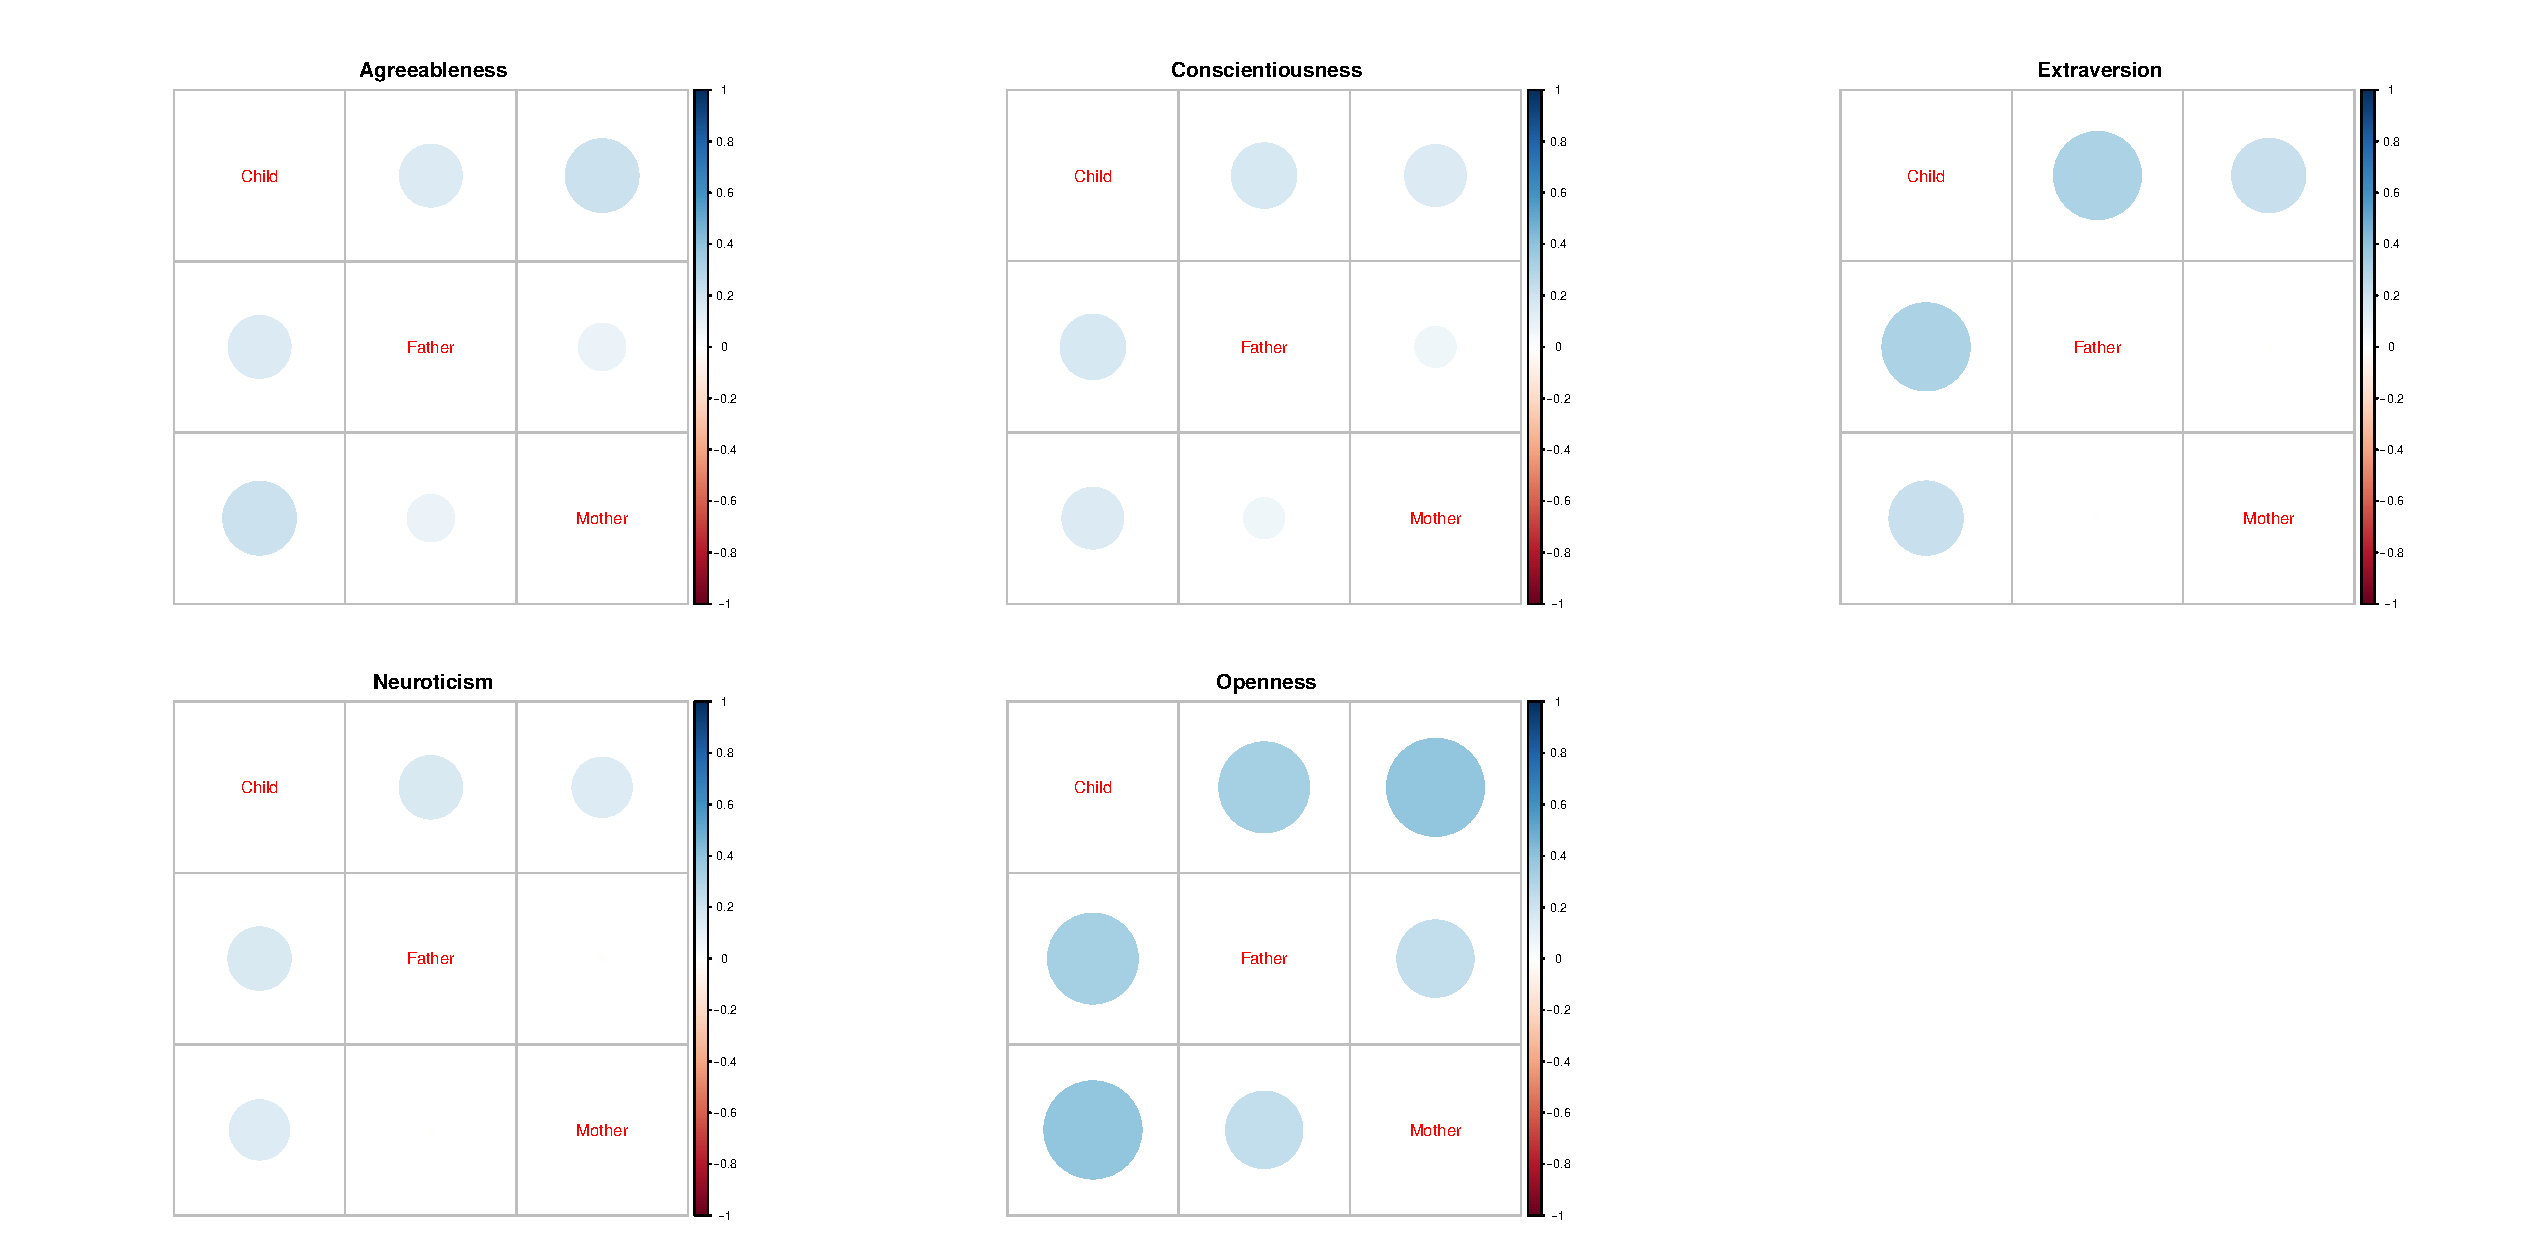
\includegraphics[width=\textwidth]{cor_separate.eps}
\caption{Estimated correlation matrix for each aspect of personality.} \label{corr_sep}
\end{figure} 


{\scriptsize{
%\begin{table}[ht]
\begin{center}
\setlength\LTleft{0pt}
\setlength\LTright{0pt}
\begin{longtable}{@{\extracolsep{\fill}}lcccccc@{}}
  \hline
CovParm & Estimate & Std & $95\%$-Lower & $95\%$-Upper & Z-value & P-value \\ 
  \hline
 A.child  & 0.183 & 0.013 & 0.158 & 0.208 & 14.421 & 0.000 \\ 
   (A.father,A.child)  & 0.028 & 0.010 & 0.008 & 0.048 & 2.784 & 0.005 \\ 
   A.father  & 0.172 & 0.008 & 0.156 & 0.187 & 21.630 & 0.000 \\ 
   (A.mother,A.child)  & 0.040 & 0.009 & 0.022 & 0.057 & 4.326 & 0.000 \\ 
   (A.mother,A.father)  & 0.015 & 0.007 & 0.002 & 0.029 & 2.303 & 0.021 \\ 
   A.mother  & 0.176 & 0.007 & 0.162 & 0.191 & 24.117 & 0.000 \\ 
   (C.child,A.child)  & 0.081 & 0.011 & 0.060 & 0.103 & 7.417 & 0.000 \\ 
   (C.child,A.father)  & 0.020 & 0.012 & -0.004 & 0.044 & 1.641 & 0.101 \\ 
   (C.child,A.mother)  & 0.008 & 0.011 & -0.014 & 0.030 & 0.712 & 0.477 \\ 
   C.child  & 0.318 & 0.018 & 0.282 & 0.354 & 17.314 & 0.000 \\ 
   (C.father,A.child)  & 0.011 & 0.011 & -0.011 & 0.033 & 0.965 & 0.334 \\ 
   (C.father,A.father)  & 0.096 & 0.006 & 0.084 & 0.108 & 15.488 & 0.000 \\ 
   (C.father,A.mother)  & 0.009 & 0.007 & -0.005 & 0.024 & 1.271 & 0.204 \\ 
   (C.father,C.child)  & 0.045 & 0.013 & 0.018 & 0.071 & 3.310 & 0.001 \\ 
   C.father  & 0.211 & 0.009 & 0.193 & 0.229 & 23.220 & 0.000 \\ 
   (C.mother,A.child)  & 0.020 & 0.010 & 0.000 & 0.039 & 2.002 & 0.045 \\ 
   (C.mother,A.father)  & 0.024 & 0.007 & 0.010 & 0.039 & 3.294 & 0.001 \\ 
   (C.mother,A.mother)  & 0.101 & 0.006 & 0.090 & 0.113 & 17.204 & 0.000 \\ 
   (C.mother,C.child)  & 0.042 & 0.012 & 0.018 & 0.065 & 3.479 & 0.000 \\ 
   (C.mother,C.father)  & 0.015 & 0.008 & -0.001 & 0.031 & 1.845 & 0.065 \\ 
   C.mother  & 0.233 & 0.009 & 0.216 & 0.250 & 26.458 & 0.000 \\ 
   (E.child,A.child)  & 0.104 & 0.012 & 0.081 & 0.126 & 8.933 & 0.000 \\ 
   (E.child,A.father)  & 0.008 & 0.013 & -0.018 & 0.033 & 0.593 & 0.553 \\ 
   (E.child,A.mother)  & -0.002 & 0.012 & -0.025 & 0.020 & -0.212 & 0.832 \\ 
   (E.child,C.child)  & 0.076 & 0.014 & 0.049 & 0.102 & 5.510 & 0.000 \\ 
   (E.child,C.father)  & 0.039 & 0.015 & 0.011 & 0.068 & 2.693 & 0.007 \\ 
   (E.child,C.mother)  & 0.018 & 0.013 & -0.007 & 0.043 & 1.434 & 0.152 \\ 
   E.child  & 0.375 & 0.020 & 0.335 & 0.414 & 18.516 & 0.000 \\ 
   (E.father,A.child)  & 0.020 & 0.013 & -0.007 & 0.046 & 1.470 & 0.142 \\ 
   (E.father,A.father)  & 0.107 & 0.007 & 0.093 & 0.122 & 14.426 & 0.000 \\ 
   (E.father,A.mother)  & 0.004 & 0.009 & -0.014 & 0.021 & 0.433 & 0.665 \\ 
   (E.father,C.child)  & 0.021 & 0.016 & -0.010 & 0.052 & 1.309 & 0.191 \\ 
   (E.father,C.father)  & 0.132 & 0.008 & 0.116 & 0.147 & 16.313 & 0.000 \\ 
   (E.father,C.mother)  & 0.012 & 0.010 & -0.008 & 0.031 & 1.180 & 0.238 \\ 
   (E.father,E.child)  & 0.116 & 0.017 & 0.083 & 0.150 & 6.804 & 0.000 \\ 
   E.father  & 0.359 & 0.013 & 0.333 & 0.385 & 27.247 & 0.000 \\ 
   (E.mother,A.child)  & 0.025 & 0.012 & 0.002 & 0.048 & 2.111 & 0.035 \\ 
   (E.mother,A.father)  & 0.003 & 0.009 & -0.014 & 0.020 & 0.338 & 0.735 \\ 
   (E.mother,A.mother)  & 0.083 & 0.007 & 0.070 & 0.097 & 11.931 & 0.000 \\ 
   (E.mother,C.child)  & -0.008 & 0.014 & -0.036 & 0.020 & -0.555 & 0.579 \\ 
   (E.mother,C.father)  & 0.010 & 0.010 & -0.008 & 0.029 & 1.099 & 0.272 \\ 
   (E.mother,C.mother)  & 0.141 & 0.008 & 0.126 & 0.157 & 17.899 & 0.000 \\ 
   (E.mother,E.child)  & 0.085 & 0.015 & 0.056 & 0.115 & 5.700 & 0.000 \\ 
   (E.mother,E.father)  & -0.000 & 0.012 & -0.023 & 0.022 & -0.039 & 0.969 \\ 
   E.mother  & 0.393 & 0.013 & 0.367 & 0.418 & 30.284 & 0.000 \\ 
   (N.child,A.child)  & -0.136 & 0.013 & -0.162 & -0.110 & -10.276 & 0.000 \\ 
   (N.child,A.father)  & -0.010 & 0.015 & -0.038 & 0.019 & -0.658 & 0.511 \\ 
   (N.child,A.mother)  & 0.017 & 0.013 & -0.009 & 0.043 & 1.253 & 0.210 \\ 
  (N,child,C.child)  & -0.069 & 0.015 & -0.099 & -0.038 & -4.446 & 0.000 \\ 
   (N.child,C.father)  & 0.007 & 0.016 & -0.025 & 0.039 & 0.413 & 0.679 \\ 
   (N.child,C.mother)  & -0.030 & 0.014 & -0.058 & -0.001 & -2.055 & 0.040 \\ 
   (N.child,E.child)  & -0.196 & 0.017 & -0.229 & -0.162 & -11.480 & 0.000 \\ 
   (N.child,E.father)  & -0.034 & 0.019 & -0.072 & 0.004 & -1.773 & 0.076 \\ 
   (N.child,E.mother)  & -0.046 & 0.017 & -0.080 & -0.013 & -2.699 & 0.007 \\ 
   (N.child,N.Child)  & 0.490 & 0.026 & 0.439 & 0.540 & 18.976 & 0.000 \\ 
   (N.father,A.child)  & -0.023 & 0.014 & -0.051 & 0.005 & -1.602 & 0.109 \\ 
   (N.father,A.father)  & -0.152 & 0.008 & -0.168 & -0.136 & -18.611 & 0.000 \\ 
   (N.father,A.mother)  & -0.004 & 0.010 & -0.023 & 0.015 & -0.403 & 0.687 \\ 
   (N.father,C.child)  & 0.019 & 0.017 & -0.015 & 0.052 & 1.079 & 0.281 \\ 
   (N.father,C.father)  & -0.124 & 0.009 & -0.141 & -0.108 & -14.577 & 0.000 \\ 
   (N.father,C.mother)  & -0.017 & 0.011 & -0.038 & 0.004 & -1.570 & 0.116 \\ 
   (N.father,E.child)  & -0.023 & 0.018 & -0.059 & 0.014 & -1.223 & 0.221 \\ 
   (N.father,E.father)  & -0.211 & 0.011 & -0.232 & -0.190 & -19.843 & 0.000 \\ 
   (N.father,E.mother)  & -0.002 & 0.013 & -0.026 & 0.023 & -0.130 & 0.897 \\ 
   (N.father, N.child)  & 0.072 & 0.021 & 0.031 & 0.113 & 3.446 & 0.001 \\ 
   (N.father,N.father)  & 0.404 & 0.015 & 0.375 & 0.434 & 26.868 & 0.000 \\ 
   (N.mother,A.child)  & -0.030 & 0.013 & -0.055 & -0.006 & -2.411 & 0.016 \\ 
   (N.mother,A.father)  & 0.000 & 0.010 & -0.018 & 0.019 & 0.031 & 0.975 \\ 
   (N.mother,A.mother)  & -0.129 & 0.008 & -0.144 & -0.114 & -16.961 & 0.000 \\ 
   (N.mother,C.child)  & -0.018 & 0.015 & -0.048 & 0.011 & -1.212 & 0.226 \\ 
   (N.mother,C.father)  & 0.002 & 0.010 & -0.018 & 0.023 & 0.240 & 0.810 \\ 
  (N.mother,C.mother)  & -0.117 & 0.008 & -0.133 & -0.101 & -14.193 & 0.000 \\ 
   (N.mother,E.child)  & -0.050 & 0.016 & -0.081 & -0.019 & -3.142 & 0.002 \\ 
   (N.mother,E.father)  & 0.008 & 0.013 & -0.017 & 0.033 & 0.647 & 0.518 \\ 
   (N.mother,E.mother)  & -0.243 & 0.011 & -0.264 & -0.222 & -22.971 & 0.000 \\ 
   (N.mother,N.child)  & 0.067 & 0.018 & 0.031 & 0.102 & 3.685 & 0.000 \\ 
   (N.mother,N.father)  & -0.001 & 0.014 & -0.028 & 0.026 & -0.060 & 0.952 \\ 
   N.mother  & 0.428 & 0.015 & 0.399 & 0.457 & 29.154 & 0.000 \\ 
   (O.child,A.child)  & 0.028 & 0.010 & 0.008 & 0.048 & 2.738 & 0.006 \\ 
   (O.child,A.father)  & -0.005 & 0.011 & -0.027 & 0.016 & -0.486 & 0.627 \\ 
   (O.child,A.mother)  & 0.002 & 0.010 & -0.018 & 0.022 & 0.201 & 0.841 \\ 
   (O.child,C.child)  & 0.026 & 0.012 & 0.003 & 0.050 & 2.173 & 0.030 \\ 
   (O.child,C.father)  & 0.015 & 0.013 & -0.010 & 0.039 & 1.172 & 0.241 \\ 
   (O.child,C.mother)  & -0.001 & 0.011 & -0.023 & 0.020 & -0.129 & 0.897 \\ 
   (O.child,E.child)  & 0.092 & 0.013 & 0.066 & 0.117 & 7.032 & 0.000 \\ 
   (O.child,E.father)  & 0.032 & 0.015 & 0.003 & 0.061 & 2.156 & 0.031 \\ 
   (O.child,E.mother)  & 0.039 & 0.013 & 0.013 & 0.065 & 2.921 & 0.003 \\ 
   (O.child,N.child)  & -0.024 & 0.014 & -0.052 & 0.004 & -1.666 & 0.096 \\ 
   (O.child,N.father)  & -0.009 & 0.016 & -0.040 & 0.022 & -0.560 & 0.576 \\ 
   (O.child,N.mother)  & -0.035 & 0.014 & -0.063 & -0.007 & -2.442 & 0.015 \\ 
   O.child  & 0.284 & 0.016 & 0.252 & 0.315 & 17.484 & 0.000 \\ 
   (O.father,A.child)  & 0.002 & 0.012 & -0.021 & 0.025 & 0.155 & 0.877 \\ 
   (O.father,A.father)  & 0.041 & 0.007 & 0.028 & 0.054 & 6.294 & 0.000 \\ 
   (O.father,A.mother)  & 0.025 & 0.008 & 0.010 & 0.041 & 3.198 & 0.001 \\ 
   (O.father,C.child)  & -0.035 & 0.014 & -0.063 & -0.008 & -2.496 & 0.013 \\ 
   (O.father,C.father)  & 0.057 & 0.007 & 0.043 & 0.071 & 8.103 & 0.000 \\ 
   (O.father,C.mother)  & 0.006 & 0.009 & -0.011 & 0.024 & 0.711 & 0.477 \\ 
   (O.father,E.child)  & 0.028 & 0.015 & -0.001 & 0.058 & 1.892 & 0.059 \\ 
   (O.father,E.father)  & 0.137 & 0.009 & 0.120 & 0.154 & 15.617 & 0.000 \\ 
   (O.father,E.mother)  & 0.010 & 0.010 & -0.010 & 0.030 & 0.966 & 0.334 \\ 
   (O.father,N.child)  & -0.016 & 0.017 & -0.049 & 0.018 & -0.931 & 0.352 \\ 
   (O.father,N.father)  & -0.065 & 0.009 & -0.083 & -0.047 & -7.179 & 0.000 \\ 
   (O.father,N.mother)  & -0.014 & 0.011 & -0.036 & 0.008 & -1.254 & 0.210 \\ 
   (O.father,O.child)  & 0.095 & 0.013 & 0.069 & 0.120 & 7.255 & 0.000 \\ 
   O.father  & 0.281 & 0.011 & 0.259 & 0.302 & 25.880 & 0.000 \\ 
   (O.mother,A.child)  & 0.026 & 0.011 & 0.005 & 0.048 & 2.386 & 0.017 \\ 
   (O.mother,A.father)  & -0.005 & 0.008 & -0.021 & 0.011 & -0.641 & 0.522 \\ 
   (O.mother,A.mother)  & 0.047 & 0.006 & 0.034 & 0.059 & 7.395 & 0.000 \\ 
   (O.mother,C.child)  & -0.006 & 0.013 & -0.032 & 0.020 & -0.460 & 0.645 \\ 
   (O.mother,C.father)  & -0.024 & 0.009 & -0.041 & -0.006 & -2.657 & 0.008 \\ 
   (O.mother,C.mother)  & 0.054 & 0.007 & 0.041 & 0.068 & 7.824 & 0.000 \\ 
   (O.mother,E.child)  & 0.014 & 0.014 & -0.013 & 0.041 & 0.993 & 0.321 \\ 
   (O.mother,E.father)  & -0.007 & 0.011 & -0.028 & 0.015 & -0.612 & 0.540 \\ 
   (O.mother,E.mother)  & 0.166 & 0.009 & 0.149 & 0.184 & 18.808 & 0.000 \\ 
   (O.mother,N.child)  & -0.017 & 0.016 & -0.048 & 0.013 & -1.105 & 0.269 \\ 
   (O.mother,N.father)  & 0.013 & 0.012 & -0.010 & 0.036 & 1.115 & 0.265 \\ 
   (O.mother,N.mother)  & -0.100 & 0.009 & -0.118 & -0.082 & -11.059 & 0.000 \\ 
   (O.mother,O.child)  & 0.117 & 0.012 & 0.093 & 0.141 & 9.487 & 0.000 \\ 
   (O.mother,O.father)  & 0.072 & 0.010 & 0.053 & 0.091 & 7.400 & 0.000 \\ 
   O.mother  & 0.314 & 0.011 & 0.292 & 0.335 & 28.862 & 0.000 \\ 
   \hline
   \caption{$D$-matrix parameter estimation (120 component $\tilde{D}$)}
\label{d_est}
\end{longtable}

\end{center}
}}




\begin{figure}
\centering
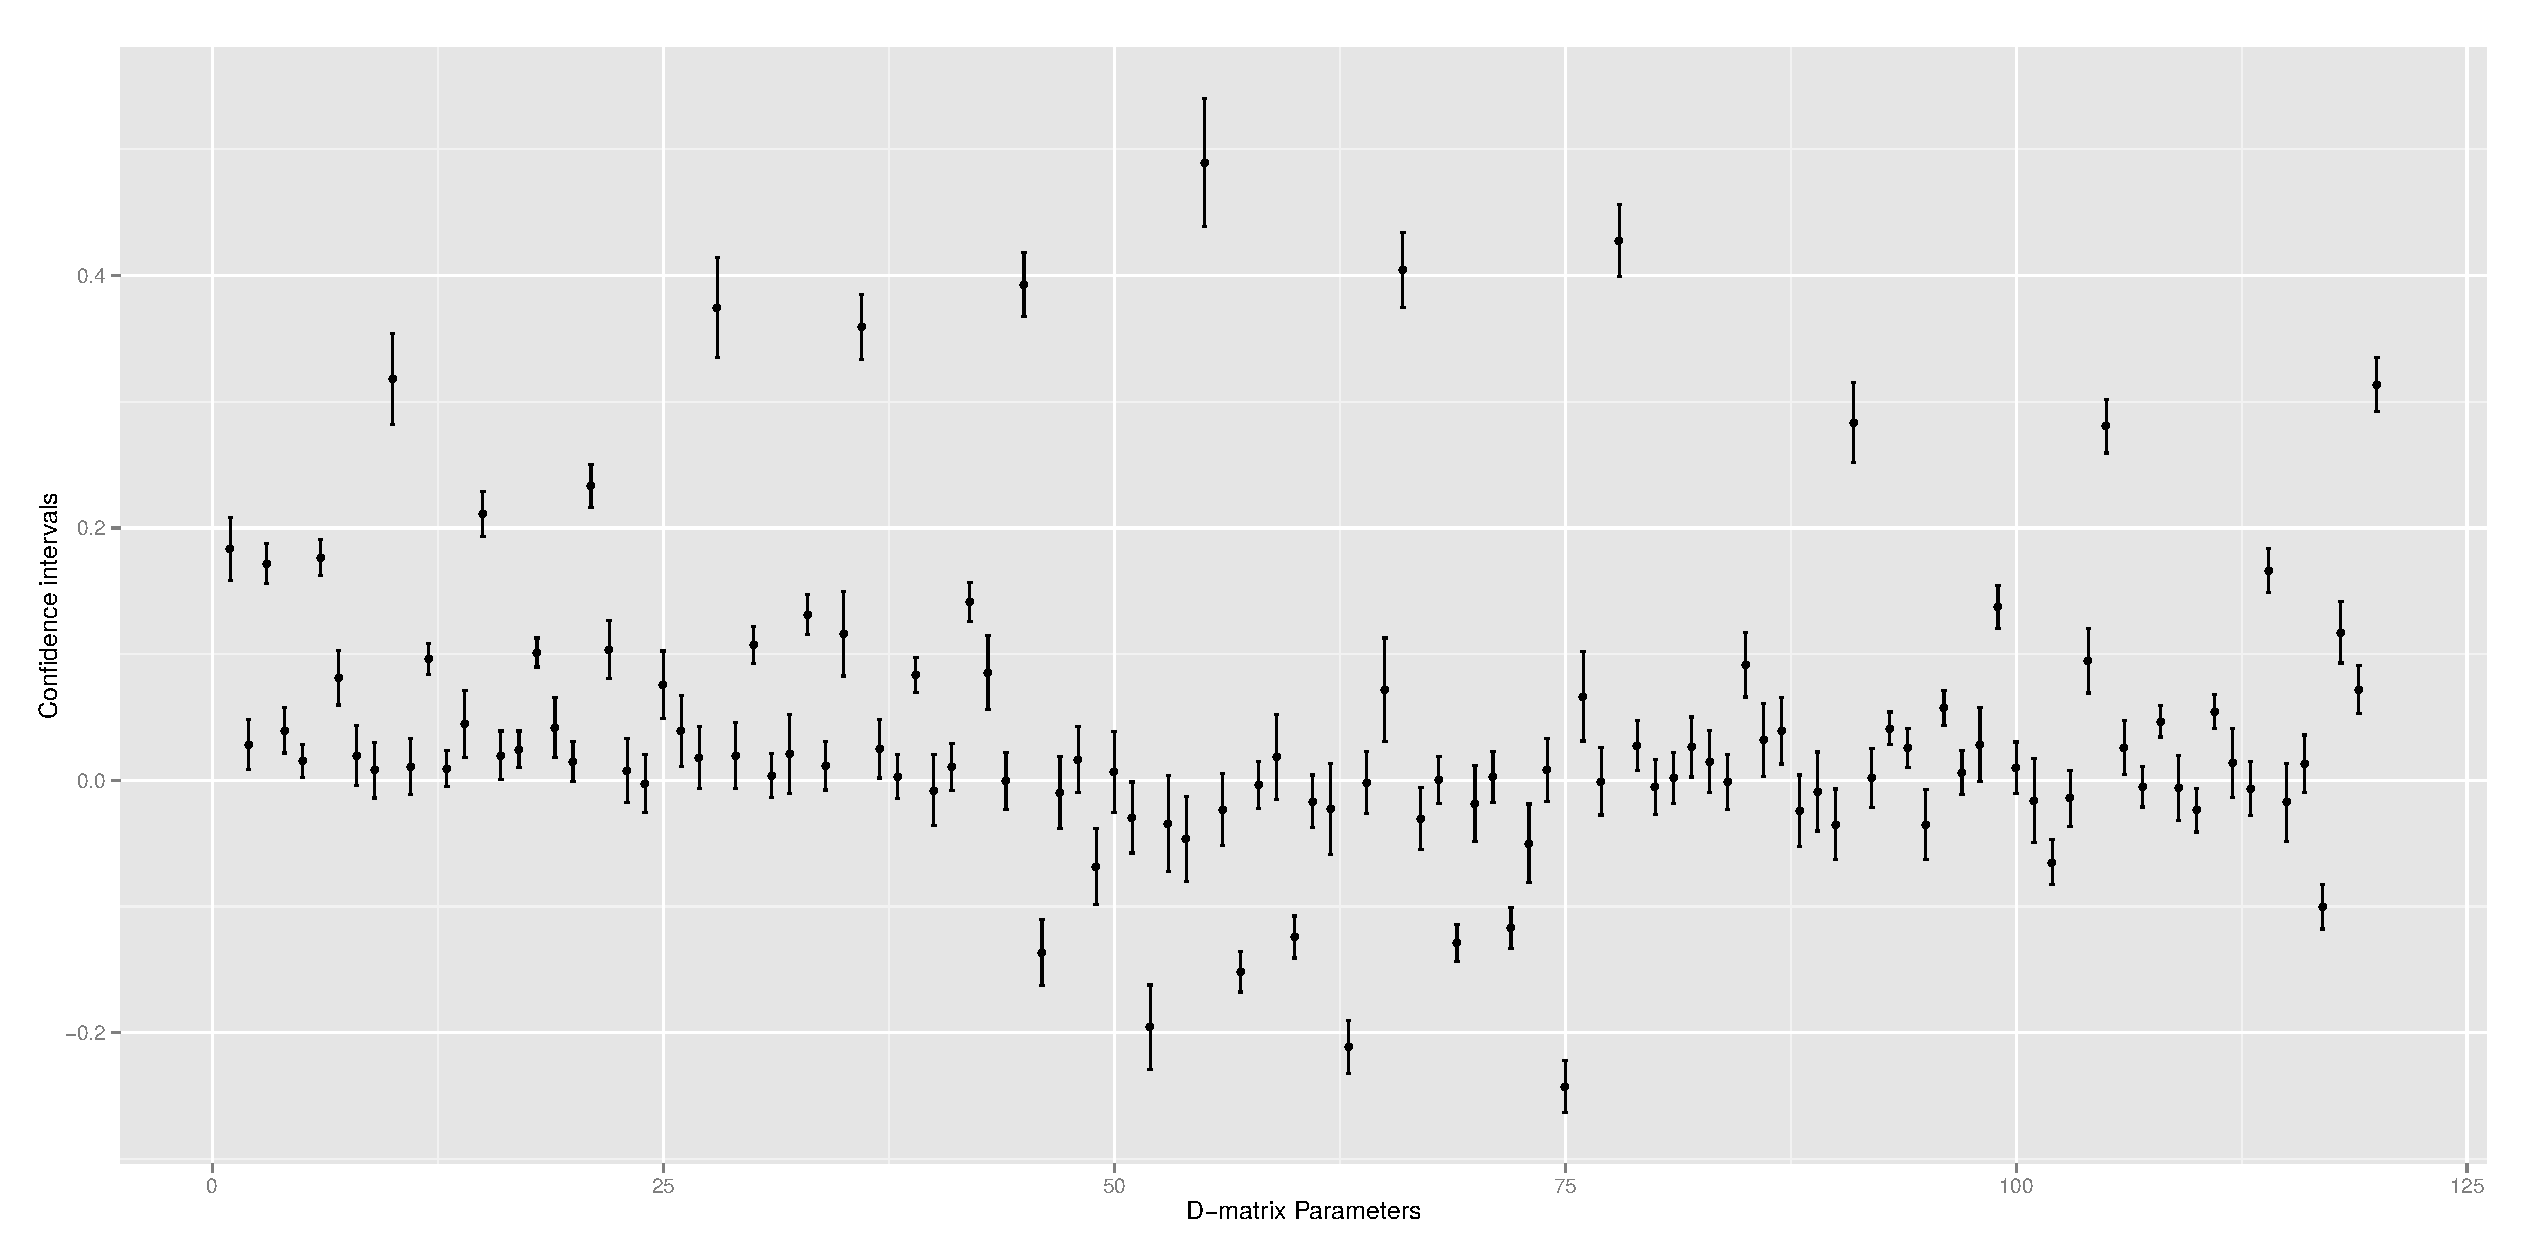
\includegraphics[width=\textwidth]{d_param.eps}
\caption{120 components of $\tilde{D}$ and their $95\%$ confidence intervals} 
\label{d_ci}
\end{figure} 

Interesting observations can be made from the results in Table~\ref{d_est}. For example, considering only the point estimates of correlations, we may see in case of Agreeableness, the correlation of mother and child is larger than the correlation of father and child. The same is true for Openness to experience. However, for Extraversion, this is larger for father than child. In case of Consciousness and Neuroticism, the correlations are more or less similar. Note that, the correlations are not that large but still comparisons would be beneficial.

\section{How precise are we?}
\label{how_good_sec}

As it was discussed, while data splitting would help the computation time, and even solve a problem that could not be solved otherwise, this all will come at a price: efficiency loss. Usually, it is not possible to quantify and study this efficiency loss, as the conventional maximum likelihood is not feasible, but one can have an idea about it by using both methods on the same problem but in a smaller scale. In this section we study the estimates using sample splitting in some sub-problems where the likelihood is feasible to compute. This way the performance of sample splitting can be compared with the full sample likelihood. 

The sub-models would still include all family roles, but the personality factors are considered separately. Therefore, each time we only have 3 outcomes of interest. Table \ref{full_split_comp} shows the results for $D$ matrix. As one may see the results of sample splitting and full sample are very similar. This would provide a greater degree of confidence in what we have obtained for all of the 15 responses using random horizontal splitting.


\begin{table}[ht]
\caption{Comparing full sample and sample splitting results for each factor separately}
\label{full_split_comp}
\centering
\resizebox{\textwidth}{!}{%
\begin{tabular}{cccccc}
& &Estimate & & Std & \\
  \hline
Factor&Parameter & Split & Full & Split & Full \\ 
  \hline
  \hline
  &  child  & 0.176 & 0.186 & 0.013 & 0.013 \\ 
    &  (father,child)  & 0.027 & 0.027 & 0.010 & 0.010 \\ 
    Agreeableness  &  father  & 0.176 & 0.170 & 0.008 & 0.008 \\ 
      &  (mother,child)  & 0.044 & 0.042 & 0.009 & 0.009 \\ 
      &  (mother,father)  & 0.021 & 0.015 & 0.007 & 0.007 \\ 
      &  mother  & 0.171 & 0.175 & 0.007 & 0.007 \\ 
   \hline
      &  child  & 0.275 & 0.320 & 0.017 & 0.018 \\ 
      &  (father,child)  & 0.044 & 0.046 & 0.013 & 0.014 \\ 
    Conscientiousness  &  father  & 0.202 & 0.210 & 0.009 & 0.009 \\ 
      &  (mother,child)  & 0.042 & 0.044 & 0.011 & 0.012 \\ 
      &  (mother,father)  & 0.019 & 0.013 & 0.008 & 0.008 \\ 
     &  mother  & 0.212 & 0.231 & 0.008 & 0.009 \\ 
  \hline
    &  child  & 0.324 & 0.374 & 0.019 & 0.020 \\ 
      &  (father,child)  & 0.076 & 0.111 & 0.016 & 0.017 \\ 
    Extraversion  &  father  & 0.298 & 0.355 & 0.012 & 0.013 \\ 
      &  (mother,child)  & 0.074 & 0.083 & 0.014 & 0.015 \\ 
      &  (mother,father)  & 0.014 & -0.000 & 0.010 & 0.012 \\ 
      &  mother  & 0.319 & 0.389 & 0.011 & 0.013 \\ 
   \hline
      &  child  & 0.400 & 0.490 & 0.023 & 0.026 \\ 
      &  (father,child)  & 0.055 & 0.064 & 0.018 & 0.021 \\ 
    Neuroticism  &  father  & 0.321 & 0.400 & 0.013 & 0.015 \\ 
      &  (mother,child)  & 0.055 & 0.061 & 0.016 & 0.018 \\ 
      &  (mother,father)  & 0.011 & -0.001 & 0.012 & 0.014 \\ 
      &  mother  & 0.346 & 0.424 & 0.013 & 0.015 \\ 
   \hline
  &  child  & 0.255 & 0.283 & 0.016 & 0.016 \\ 
      &  (father,child)  & 0.070 & 0.095 & 0.012 & 0.013 \\ 
    Openness  &  father  & 0.245 & 0.278 & 0.010 & 0.011 \\ 
      &  (mother,child)  & 0.095 & 0.119 & 0.012 & 0.012 \\ 
      &  (mother,father)  & 0.063 & 0.071 & 0.009 & 0.010 \\ 
      &  mother  & 0.269 & 0.311 & 0.010 & 0.011 \\ 
   \hline
\end{tabular}}

\end{table}
%use the report in "D:\GOOD\BFI\personality_report": 


\chapter{Structured horizontal splitting}
\label{chap_struc_horiz}
\section[Compound-symmetry structure]{Clusters with unequal size: Maximum likelihood versus weighted estimation in large samples}
\label{sec_cs}
\subsection{Introduction}
\label{secintrocs}

Much statistical theory is derived under the paradigm of a fixed sample size. However, there are many common practical settings in which this paradigm does not hold. Examples include sequential trials, where the trial may be stopped early at a number of time points during accrual, because of the strength, or lack, of a treatment effect; incomplete data in longitudinal studies or surveys; longitudinal data with random measurement occasions; and censored survival data.
\cite{molenberghs2014random} provide an overview of such situations.

Here, we focus on hierarchical (or clustered) data with unequal cluster sizes.

Clustering is taken in its broadest sense, encompassing longitudinal data, family-based studies, toxicology (\cite{aerts2002}), agricultural experiments, multi-level designs in the social and behavioral sciences, and so on. In longitudinal trials, it is not uncommon to plan for the same number of measurements to be taken per study subject, often at a common set of time points. If all data were collected according to protocol, the cluster size would be fixed. However, even in such studies, cluster sizes are often {\em de facto\/} random because of incompleteness in the data. In many random cluster size settings there may be associations between outcomes and cluster size. In part of the literature, this is termed `informative cluster size' and a suite of methods has been proposed to accommodate this situation, many based on inverse probability weighting \citep{williamson2003marginal, benhin2005mean, hoffman2001, cong2007marginal, chiang2008efficient, wang2011inference, aerts2011incomplete}. Unequal cluster sizes can occur for any outcome type, including continuous, binary, categorical, count, and event time.


%(Williamson, Datta, and Satten (2003); Benhin, Rao, and Scott (2005); Hoffman, Sen, and Weinberg (2001); Cong, Yin, and Shen (2007); Chiang and Lee (2008); Wang, Kong, and Datta (2011); Aerts {\it et al.} (2011)).
%\cite{williamson2003marginal, benhin2005mean, hoffman2001, cong2007marginal, chiang2008efficient, wang2011inference, aerts2011incomplete. 



Unequal cluster sizes may or may not be governed by a stochastic mechanism. For example, they can be unequal by design choice, without being stochastic; e.g., when a sample is selected in each town proportion to the population size. Litter sizes in pregnant rodents will truly be stochastic. When stochastic, the mechanism is completely random when it depends on neither observed nor unobserved data; it is random when it depends on observed but, given these, not on unobserved data; other mechanisms are termed non-random. In the literature, mechanisms other than complete random are often termed informative. Although an important issue, we do not focus on informative cluster sizes here. Attention is confined to the case where cluster size is unequal, but independent of both observed and unobserved outcomes. In doing so we distinguish issues that stem purely from the non-constant nature of the cluster size, from those that result from the association between cluster size and outcome. We focus on the differences between the case of a fixed cluster size that is common to all clusters, and that of a fluctuating cluster size, whether for design reasons or randomly. In particular, the joint modelling of outcomes and cluster size is not considered.

As a simple, yet non-trivial, clustering paradigm, we consider the normal compound-symmetry (CS) model, which is a three-parameter multivariate normal model, with a common mean $\mu$, a common variance $\sigma^2+d$, and a common covariance $d$.  \cite{Iddi2011} studied this case in the context of so-called split-sample methodology: they proposed a particular form of pseudo-likelihood where a sample is subdivided into $M$ subsamples, which are separately analyzed as if they were unrelated, after which the results are averaged using appropriate weights, leading to proper point and precision estimates. 
Pseudo-likelihood has received considerable attention \citep[Ch.~9, 12, 21, 24, 25)]{molenberghs2005}; \citep[Ch.~6, 7]{aerts2002}.


%Molenberghs and Verbeke (2005, Ch.~9, 12, 21, 24, 25); Aerts {\em et al.\/} (2002, Ch.~6, 7)

Assume that there are $c_k$ clusters of size $n_k$, $k=1,\dots,K$. For ease of development, we allow for some of the $n_k$ to be equal, which is useful when a subgroup of clusters that is of the same size is chosen to be sub-divided (because there are very many or for other reasons). A natural split is made with respect to the cluster size, i.e., as if every cluster size defines its own stratum. 

Evidently, for medium to large sample sizes, full maximum likelihood or Bayesian inferences are statistically optimal and computationally feasible; hence, the work done here might be less relevant. However, with really big data, where the number of independent clusters runs in the millions or beyond, and/or in settings where the number of measurements per cluster becomes very large (e.g., in meta-analysis), maximum likelihood eventually becomes prohibitive in terms of computation time. At the other end of the spectrum, in very small samples (e.g., in small-area epidemiology applications, or when studies are conducted in so-called orphan diseases), maximum likelihood estimates may become unstable, to the point where it is difficult to obtain convergence.  This may be due, for example, to relatively flat likelihood functions. The non-iterative nature of our proposal removes such issues. Small samples refers here to a small number of clusters; the clusters themselves may consist of smaller or larger numbers of within-cluster replication. 
We are not the first to consider these issues. \cite{wim2015} considered multiple imputation to bring clusters to the same size before applying maximum likelihood. If done with care, convergence problems are drastically reduced. \cite{williamson2003marginal} and \cite{follmann2003} proposed so-called multiple outputation, to repeatedly create independent samples by randomly selecting one member per cluster.  To ensure that correlation is taken into account, combination rules reminiscent of multiple imputation are then applied to combine inferences from the samples drawn. These methods are based on repeated sampling and  come at computational cost for high-dimensional data (\cite{sikorska2013_2}). Therefore, in this paper, the focus is on entirely non-iterative methods, bringing together the advantages of balanced data and simple averaging methodology. A consequence of our approach is the need for applying weights when combining results from the $K$ strata.  We establish how results on incomplete sufficient statistics in the context of weighted averages \citep{molenberghs2014random, Lisa2015_2} imply that there may be no optimal set of weights. Given this, we propose pragmatically attractive weights, in terms of efficiency, bias, and computational ease.

The remainder of the paper is organized as follows. Two motivating datasets are described in Section~2.
%\ref{dataintro}.
In Section~3
%\ref{incompleteness} 
essential background material on incomplete sufficient statistics is presented. The compound-symmetry model is introduced in Section~4,
%\ref{model}
and a review is provided of the relevant incompleteness results from \cite{Lisa2015_2}, together with implications for likelihood-based estimation. Background from the pseudo-likelihood-based split-sample method is given in Supplementary Material Section~S.4.
%\ref{splitsample}
A general split-sample approach to the CS model is provided in Section~5,
%\ref{CSsplitsample}
and a number of specific but practically relevant cases are considered.
Details about the specifics for the CS case are presented in Section~6.
%\ref{psa7}.
Section~7
%\ref{simulation}
 is dedicated to a simulation study, examining situations for which there are no closed forms on the one hand, and studying numerical performance (speed and convergence) on the other. The data, described in Section~2,
%\ref{dataintro}
are analyzed in Section~8.
%\ref{dataanal}
Ramifications and recommendations for practice are offered in Section~9.
%\ref{ramifications}.

%\setcounter{section}{2} %***
%\setcounter{equation}{0} %-1
\subsection{Developmental Toxicity Study Sets}
%\label{dataintro}
\label{ntpintro}

Data from the Research Triangle Institute under contract to the National Toxicology
Program of the U.S.A. (NTP data), are analyzed. These developmental toxicity
studies investigate the effects in mice of three chemicals: di(2-\-ethylhexyl)phthalate (DEHP)  \citep{tyl1988}
ethylene glycol (EG) \cite{price1985}, and  diethylene glycol dimethyl ether (DYME) 
\cite{price1987developmental}.  The studies were conducted in timed-pregnant mice during the period of major organogenesis. The dams were sacrificed, just prior to normal delivery, and  the status of uterine implantation sites recorded. The outcome of interest here is fetal weight. 
Summary data from the  DEHP trial are presented in Table~\ref{tabclus}. The design for EG and DYME is similar. 
It is clear from the table that average litter size is depleted with increasing dose, as is the average weight.\addtolength{\tabcolsep}{2mm}
\begin{table}[t!]
\begin{center}
\caption{\small \linespread{1.1}  Developmental Toxicity Study (DEHP). Summary data by dose group.}
\label{tabclus}
\centerline{\def\arraystretch{0.6}\tabcolsep=3truept\begin{tabular}{rccccc}
\hline
\hline
\multicolumn{1}{c}{}&
\multicolumn{2}{c}{\# dams with}&
\multicolumn{1}{c}{\# live}&
\multicolumn{2}{c}{average}
\\
\cline{2-3}\cline{5-6}
\multicolumn{1}{c}{dose}&
\multicolumn{1}{c}{implants}&
\multicolumn{1}{c}{viable implants}&\multicolumn{1}{c}{fetuses}&
\multicolumn{1}{c}{litter size}&
\multicolumn{1}{c}{weight}\\
\hline
  0 mg/kg/day&30&30&330&13.2&0.9483\\
 44 mg/kg/day&26&26&288&11.1&0.9592\\
 91 mg/kg/day&26&26&277&10.7&0.8977\\
191 mg/kg/day&24&17&137&\phantom{9}8.1&0.8509\\
292 mg/kg/day&25&\phantom{9}9&\phantom{9}50&\phantom{9}5.6&0.6906\\
\hline
\hline
\end{tabular}}
\end{center}
\end{table}
\addtolength{\tabcolsep}{-2mm}

%%%%%%%%%%%%%%%%%%%%%%%%%%%%%%%%%%%%%%%%%%%%%%%%%%%%%%%%%%%%%%%%%%%%%%%%%%%%%%%%%%%%%%%%%%%%%%%%%%%%%%%%%%%%%%%%%%%%%%%%%%%%

\lhead[\footnotesize\thepage\fancyplain{}\leftmark]{}\rhead[]{\fancyplain{}\rightmark\footnotesize\thepage}%Put this line in Page 2



\subsection{Incomplete Sufficient Statistics}\label{incompleteness}

A statistic $k(Y)$ of a random variable $Y$, with $Y$ belonging to a family $P_\theta$, is complete if, for every measurable function $g(\cdot)$, independent of $\theta$, $E[g\{k(Y)\}]=0$ for all $\theta$, implies that  $P_\theta[g\{k(Y)\}=0]=1$  for all $\theta$  \citep{casella2002statistical}. The Lehman-Scheff\'e\ theorem \citep{casella2002statistical} states that, if a statistic is unbiased, complete, and sufficient for a parameter $\theta$, then it leads to the best mean-unbiased estimator for $\theta$, while Basu's theorem  \citep{basu1955statistics} has it that statistic that is both boundedly complete and sufficient is independent of any ancillary statistic.  As has been shown in the sequential trial context, a lack of completeness does not preclude the existence of estimators with very good properties  \citep{molenberghs2014random}.

\cite{liu1999unbiased} established the incompleteness of the sufficient statistic for a clinical trial with a stopping rule, for the case of normally distributed endpoints. \citet{liu1999unbiased} generalized this result to the entire exponential family. \citet{molenberghs2014random} and \citet{milanzi2016properties} broadened it further to a stochastic rather than a deterministic stopping rule, hence encompassing the case of a completely random sample size. Indeed, it would seem at first sight that this latter case is standard, because the sample size is unrelated to the data, whether observed or not. Yet, even in this case, completeness no longer holds. What is more, incompleteness holds when the cluster size is non-constant for whatever reason.


\subsection{The Compound-symmetry Model}
\label{model}

Let $\BY$ be a vector of length $n$, with $\BY\sim N(\mu\mathbf{1}_n,\sigma^2 I_{n}+d J_{n})$. In general, both $\BY$ and $n$ are random variables.

Suppose that there is a sample of $N$ independent clusters, among which $K$ different cluster sizes $n_{k}$ ($k=1,\dots,K$) are distinguished. Let the multiplicity of cluster size $n_k$ be equal to $c_k$. Evidently, $N=\sum_{k=1}^Kc_k$. Denote the outcome vector for the $i$th  ($i=1,\dots,c_k$) replicate among the clusters of size $n_k$ by $\BY_i^{(k)}$. We first show incompleteness of the sufficient statistic, then turn to likelihood estimation. For both, we start from the log-likelihood function. 

\subsubsection{Incompleteness}

The data-dependent terms in the log-likelihood can  be written as:
\begin{equation}
\label{driestats}
\begin{aligned}
\lefteqn{\sum_{k=1}^K\sum_{i=1}^{c_k}-\frac{1}{2}\left(\BY_i^{(k)}-\mu\mathbf{1}_{n_k}\right)'\left(\sigma^2I_{n_k}+dJ_{n_k}\right)^{-1}\left(\BY_i^{(k)}-\mu\mathbf{1}_{n_k}\right)}\\
&=&\sum_{k=1}^K\sum_{i=1}^{c_k}-\frac{1}{2}\left(\BY_i^{(k)}-\mu\mathbf{1}_{n_k}\right)'\left(I_{n_k}-\frac{d}{\sigma^2+n_kd}J_{n_k}\right)\left(\BY_i^{(k)}-\mu\mathbf{1}_{n_k}\right)\\
&=&
\sum_{k=1}^K\sum_{i=1}^{c_k}\frac{\mu}{\sigma^2+n_kd}\left(\sum_{j=1}^{n_k}Y_{ij}^{(k)}\right)
-\frac{1}{2\sigma^2}
\left(\sum_{k=1}^K\sum_{i=1}^{c_k}\sum_{j=1}^{n_k}Y_{ij}^{(k)2}\right)  \\
&+&
\sum_{k=1}^K\sum_{i=1}^{c_k}\frac{d}{2\sigma^2(\sigma^2+n_kd)}\left(
\sum_{j=1}^{n_k}Y_{ij}^{(k)}
\right)^2.
\end{aligned}
\end{equation}
The three terms in (\ref{driestats}) are qualitatively different. Indeed, the middle one corresponds to a single sufficient statistic, the sum of all squares across clusters, while the first and last split into as many sufficient statistics as there are unique cluster sizes.

\cite{Lisa2015_2} proved a characterization of incompleteness, essentially stating that when the dimension of the sufficient statistic is larger than the dimension of the parameter vector, the sufficient statistic is no longer complete. More details can be found in Supplementary Materials Section~S1.
%\ref{appA}. 
This sharp division also occurs when studying certain properties of the maximum likelihood estimator.

\subsubsection{Likelihood-based Estimation of the CS Model}
\label{likelihood}

Similar in spirit to (\ref{driestats}), but now using all terms, the log-likelihood can be written as
\begin{equation}
\label{loglikcs}
\ell(\mu,\sigma^2,d)=\sum_{k=1}^K\ell_k(\mu,\sigma^2,d),
\end{equation}
with the cluster size specific log-likelihood term


\begin{equation}
\label{loglikcsk}
\begin{aligned}
&&\ell_k(\mu,\sigma^2,d)=
-\frac{1}{2}\sum_{i=1}^{c_k}
\left\{\ln
\left[\sigma^{2n_k}+n_k\sigma^{2(n_k-1)}d\right]\phantom{\frac{d_m}{\sigma_m^2+nd_m}}
\phantom{-\frac{1}{2}\sum_{i=1}^N} \right.\\
&+&\left.(\BY_{i}^{(k)}-\mu\mathbf{1}_{n_k})'\frac{1}{\sigma^2}\left(I_{n_k}-\frac{d}{\sigma^2+n_kd}J_{n_k}\right)(\BY_{i}^{(k)}-\mu\mathbf{1}_{n_k})\right\}.
\end{aligned}
\end{equation}


Using derivations similar to those in \cite{Iddi2011}, the cluster size specific log-likelihood can be maximized analytically {\em assuming that there is a separate parameter per cluster size}. By replacing $\ell_k(\mu,\sigma^2,d)$ by
$\ell_k(\mu_k,\sigma^2_k,d_k)$, we can consider the kernel of the log-likelihood, in general for $K$ cluster sizes, and allowing for the parameter vector to change with cluster size:
\begin{equation}
   \label{jloglik}
\begin{aligned}
\ell\left(\left\{\mu_k\right\}_k,\left\{\sigma_k^2\right\}_k,\left\{d_k\right\}_k\right)  &\propto& - \frac{1}{2}\sum_{k=1}^K\sum_{i=1}^{c_k} \left\{\ln|\Sigma_{n_k}| \right. \\ 
&+& \left. \left(\by_{i}^{(k)}-\bmu_{n_k}\right)'\Sigma_{n_k}^{-1} \left(\by_{i}^{(k)}-\bmu_{n_k}\right) \right\},
\end{aligned}
\end{equation}
where $\bmu_k=\mu_k\mathbf{1}_{n_k}$  $\Sigma_{n_k}=\sigma_k^2 I_{n_k}+ d_k J_{n_k}$. The score functions are presented in Supplementary Materials Section~S.2.
%\ref{likelihoodapp}.
Solving these score functions (S2.1)-(S2.3)
%(\ref{jscore1})--(\ref{jscore3}) 
leads to:
\begin{eqnarray}
\label{muk}
\widehat{\mu}_k&=&\frac{1}{c_kn_k}\sum_{i=1}^{c_k}\sum_{j=1}^{n_k}Y_{ij}^{(k)},\\[2mm]
\widehat{\sigma}^2_k&=&\frac{1}{c_kn_k(n_k-1)}\left(
n_k\sum_{i=1}^{c_k}\BZ_{i}^{(k)'}\BZ_{i}^{(k)}-\sum_{i=1}^{c_k}\BZ_{i}^{(k)'}J_{n_k}\BZ_{i}^{(k)}
\right),\label{sigmak}\\[2mm]
\widehat{d}_k&=&
\frac{1}{c_kn_k(n_k-1)}\left(
\sum_{i=1}^{c_k}\BZ_{i}^{(k)'}J_{n_k}\BZ_{i}^{(k)}-\sum_{i=1}^{c_k}\BZ_{i}^{(k)'}\BZ_{i}^{(k)}
\right),\label{dk}
\end{eqnarray}
where $\BZ_{i}^{(k)}=\left(\BY_{i}^{(k)}-\mu_k\mathbf{1}_{n_k}\right)$.

When the cluster size is constant, the compound-symmetry model has closed form ML estimators, given by (\ref{muk})--(\ref{dk}). Closed-form estimators for the variance-covariance matrix of the estimator exist as well \citep{Iddi2011}. For the mean, the variance is:
\begin{equation}
\label{varexprmuk}
\mbox{var}(\widehat{\mu_k})=\frac{\sigma_k^2+n_kd_k}{c_kn_k}.
\end{equation}
The expressions for the variance-covariance structure of $(\widehat{\sigma^2_k},\widehat{d_k})$ is:
\begin{equation}
\label{varexprsigmakdk}
\mbox{var}\left(\begin{array}{c}\widehat{\sigma^2_k}\\ \widehat{d_k}\end{array}\right)=
\frac{2\sigma^4_k}{c_kn_k(n_k-1)}
\left(
\begin{array}{cc}
n_k&-1\\
-1&\frac{\sigma_k^4+2(n_k-1)d_k\sigma_k^2+n_k(n_k-1)d^2_k}{\sigma_k^4}
\end{array}
\right).
\end{equation}
The mean parameter is independent of the variance components.

These results can be used when a separate parameter vector is estimated for each of the cluster sizes and, as a special case,  when there is only one cluster size. Four features of use in what follows are: (a) there are closed forms; (b) the sufficient statistic is complete; (c) the estimator is unique minimum variance unbiased; (d) the mean parameter estimator and the variance parameter estimator are independent.

These results are lost when $K\ge 2$. We briefly sketch the lack of closed-form solutions in this case in Supplementary Materials Section~S2.2.
%\ref{twodifferent}.

The lack of a closed form is well known, but we highlight a few relevant features here. More detail is given in Supplementary Materials Section~S3,
%\ref{appB}, 
where we show
\begin{equation}
\widehat{\mu}
=
\frac
{
\sum_{k=1}^K\frac{n_k c_k}{\sigma^2+n_k d} \widehat{\mu_k}
}
{
\sum_{k=1}^K\frac{n_k c_k}{\sigma^2+n_k d}
}.
\label{mulik}
\end{equation}
Examining (\ref{mulik}) suggests weighted averages:
\begin{equation}
\label{weightavermu}
\widetilde{\mu}=\sum_{k=1}^Ka_k\widehat{\mu_k},\qquad
\widetilde{\sigma^2}=\sum_{k=1}^Kb_k\widehat{\sigma^2_k},\qquad
\widetilde{d}=\sum_{k=1}^Kg_k\widehat{d_k}.
\end{equation}
This idea is  similar to that in \cite{Iddi2011}, who split a sample in sub-samples, analyzed each  separately, and then combined the result in an overall estimator. They considered splits in both dependent and independent sub-samples. Dependent samples occur when very long sequences of repeated measures are collected, which are then sub-divided for convenience. This approach is not of use here. Independent samples arise when there are many independent replicates, i.e., a large number of clusters. They studied the CS case, but only for a single cluster size. The total number of clusters was then split into $M$ parts comprising an equal number of clusters. We modify these ideas to the case of unequal cluster sizes, with a variable number of clusters per split.

\subsection{Split-sample Methods for Clusters of Variable Size}
\label{CSsplitsample}

The derivations are based on general pseudo-likelihood principles, reviewed in Supplementary Materials Section~S4.
%\ref{splitsample}. 
We first make generic the setting at the beginning of Section~\ref{model}. 
Let there be a sample of $N$ independent clusters. Partition the 
sample into $K$ sub-samples, with $c_k$ independent and identically 
distributed clusters in sub-sample $k$; $N=\sum_{k=1}^Kc_k$. 
$\BY_i^{(k)}$ remains the outcome vector for replicate $i$ in 
sub-sample $k$.

Subjects in different sub-samples are allowed to have 
the same distribution, but subjects in the same sub-sample 
{\em must\/} have the same distribution. This covers the running 
example of CS clusters, partitioned according to cluster size. 
However, it is possible to further sub-divide such a sub-sample 
in various sub-samples, all with the same cluster size. This is 
sensible, for example, in very large databases. An extreme example 
follows when sub-samples consist of a single independent replicate, useful, for example, in a meta-analysis with large individual 
studies. This limiting situation can also be considered with CS data, 
because all clusters (except those of size 1) contribute to all three 
parameters.

Consider pseudo-likelihood  in this general case (see also Eq.~(S4.4)).
%(\ref{ourgenpl})]. 
Assume that $\bftheta^\ast$ is a vector of length $p$, and that 
each $\bftheta_k$ is a separate copy of $\bftheta^\ast$. Then 
it can be shown that the generic combination 
rules are 
\begin{eqnarray}
\label{schattergeneric}
\widetilde{\bftheta}^*&=&\sum_{k=1}^KA_k\widehat{\bftheta}_k,\\
\label{asymptoticgeneric}
\mbox{var}(\widetilde{\bftheta}^*)&=&\sum_{k=1}^KA_kV_kA_k',
\end{eqnarray}
with
$V_k=I_0({\bftheta}_k)^{-1}$. We use the symbol $\widetilde{\bftheta}^*$ to emphasize that this is not necessarily the maximum likelihood estimator even though, in our formalism, $\widehat{\bftheta}_k$ is the maximum likelihood estimator when restricting attention to sub-sample~$k$. 
Equation (\ref{asymptoticgeneric}) is appropriate only when the weights 
$A_k$ are free of the parameters to be estimated. We return to this at 
the end of the section.

\noindent {\bf Weighting Schemes}
Not every choice of the $A_k$ leads to an unbiased estimator. To enforce 
unbiasedness, consider the requirement
$$\bftheta=E\left(\widehat{\bftheta}^*\right)=\sum_{k=1}^KA_kE\left(\widehat{\bftheta}_k\right)=
\left(\sum_{k=1}^KA_k\right)\bftheta,$$
whence $I_p=\sum_{k=1}^KA_k$. This requirement is satisfied for (S4.5).
%(\ref{amtrix}).
This suggests two obvious choices:
\begin{description}
\item[Constant weights.] Set $A_k=(1/K)I_{p}$.
\item[Proportional weights.] Set $A_k=(c_k/N)I_p$.
\end{description}
Constant weights are the clear choice when all subjects are i.i.d.\ 
and partitioning is in sub-samples of equal size. Proportional weights 
are called for in the i.i.d.\ case,  with sub-samples of varying size.

Consider optimal weights through the objective function
$$Q=\sum_{k=1}^KA_kV_kA_k'-\Lambda\left(\sum_{k=1}^KA_k-I_p\right),$$
where $\Lambda$ is a matrix of Lagrange multipliers.
Taking the first derivative of $Q$ w.r.t.\ $A_k$ leads 
to $A_k=\Lambda V_k^{-1}/2$. Because the $A_k$ sum to the 
identity,  $\Lambda=2\left(\sum_{m=1}^KV_m^{-1}\right)^{-1}$ 
and we have the following.
\begin{description}
  \item[Optimal weights.] These take the form:
\begin{equation}
\label{optimalwt}
A_k^{\mbox{\scriptsize opt}}=\left(\sum_{m=1}^KV_m^{-1}\right)^{-1}V_k^{-1}.
\end{equation}
\end{description}
With this choice, (\ref{schattergeneric})--(\ref{asymptoticgeneric}) become:
\begin{eqnarray}
\label{schatteropt}
\widetilde{\bftheta}^*=\widehat{\bftheta}^*&=&
\left(\sum_{k=1}^KV_k^{-1}\right)^{-1}
\sum_{k=1}^KV_k^{-1}\widehat{\bftheta}_k
,\\
\mbox{var}(\widetilde{\bftheta}^*)&=&V\ =\ \left(\sum_{k=1}^KV_k^{-1}\right)^{-1}.
\label{asymptoticopt}
\end{eqnarray}
The optimal weights lead to the maximum likelihood estimator. To apply the 
optimal weights in practice is typically not straightforward. A closed form expression for the $V_k$ does not always exist, and even if it did, as in the CS case, it may depend on the 
unknown parameters. The optimal weights can suggest 
sensible choices and we describe a couple of these. They will be illustrated 
in the next section for the CS case.

{\bfseries Scalar weights.} While optimal weights 
may be unwieldy, one could consider scalar weights by requiring the $A_k$ 
to be diagonal. This implies that each component of 
$\bftheta^\ast$, $\theta_r^\ast$, say, is a linear combination
$$\widetilde{\theta}_r^\ast=\sum_{k=1}^Ka_{k,r}\widehat{\theta}_{k,r},$$
where then, formally, $A_k=\mbox{diag}(a_{k,1},\dots,a_{k,p})$. 
The optimization route, followed for unrestricted $A_k$, can then 
be followed component-wise as well. Because the class of 
$A_k$ over which to optimize is restricted, the resulting optimum 
does not necessarily correspond to the maximum likelihood solution. 
The rationale for choosing this route is computational convenience, and its advantages  
vary from problem to problem. 

{\bfseries Iterated optimal weights.} An iterative 
scheme can be followed:
\begin{enumerate}
\item Estimate $\widehat{\bftheta}_k$.
\item Compute an initial estimator for $\bftheta^\ast$, $\bftheta^{\ast(0)}$, say, using a simple weighting method, e.g., using constant or proportional weights.
\item Using the current parameter estimate, $\bftheta^{\ast(t)}$ say, calculate $V_{k}^{(t+1)}$.
\item Determine:
$$
{\bftheta}^{\ast(t+1)}=
\left(
\sum_{k=1}^K\left[V_{k}^{(t+1)}\right]^{-1}
\right)^{-1}
\sum_{k=1}^K\left[V_{k}^{(t+1)}\right]^{-1}\widehat{\bftheta_k}
.
$$
\item Repeat steps 2--3 until convergence.
\end{enumerate}
This scheme can always be followed and it has the advantage that the data 
need only be analyzed once, to yield $\widehat{\bftheta}_k$. From this point on, 
calculations involve algebraic expressions for the parameters only.

{\bfseries Approximate optimal weighting.} Related to the previous 
method, a non-iterative approximation consists of replacing 
$V_k$ by $V_k(\widetilde{\bftheta_k})$ in (\ref{schatteropt}). 
Here, $\widetilde{\bftheta_k}$ could be, for example,  the 
sub-sample specific estimator $\widehat{\bftheta_k}$, or the  
$\widetilde{\bftheta^\ast}$ obtained using a simple scheme, 
such as constant or proportional weighting. This method avoids 
all further iteration, once the $\bftheta_k$ have been determined.

Approximate optimal weighting is a method that could be considered when
the use of  (\ref{asymptoticgeneric}) might lead to underestimation of the 
variability, because the $A_k$ now depend on the parameters 
estimated from stratum~$k$. To properly account for this 
extra source of uncertainty. Consider that
\begin{equation}
\label{eerstevgl}
\frac{\partial}{\partial\bftheta_k}(A_k\bftheta_k)=A_k+
\left(
\left.
\frac{\partial A_k}{\partial\theta_{k1}}\bftheta_k\right|
\cdots
\left|
\frac{\partial A_k}{\partial\theta_{kp}}
\right.\bftheta_k
\right),
\end{equation}
where $\theta_{kj}$, $j=1,\dots,p$ ranges over the components of 
$\bftheta_k$.  Writing $W_k=V_k^{-1}$ for ease of notation,
\begin{equation}
\frac{\partial A_k}{\partial\theta_{kj}}=W^{-1}\frac{\partial W_k}{\partial\theta_{kj}}(I_p-W^{-1}W_k),
\label{tweedevgl}
\end{equation}
with $I_p$ the $p$-dimensional identity matrix. Plugging (\ref{tweedevgl}) 
into (\ref{eerstevgl}), the proper delta-method approximation to the 
variance is
\begin{equation}
\label{asymptoticgenerictwee}
\mbox{var}(\widetilde{\bftheta}^*)\simeq
\sum_{k=1}^K(A_k+B_k)V_k(A_k+B_k)',
\end{equation}
with
$$
B_k=(\mbox{\bfseries 1}_p'\otimes I_p)(I_p\otimes W^{-1})\mbox{diag}\left(
\frac{\partial W_k}{\partial\theta_{k1}},\dots,
\frac{\partial A_k}{\partial\theta_{kp}}
\right)
\left[I_p\otimes(I_p-W^{-1}W_k)\bftheta\right],
$$
and $\otimes$ signifying Kronecker product.



\subsection{Partitioned-sample Analysis for the Compound-symmetry Model}
\label{psa7}

For the normal compound-symmetry model,
%\ref{model}, 
a variety of options exists. We  sketch them here, and then 
consider some in greater detail.

Consider the i.i.d.\ case, where all clusters are of the same size. 
Full maximum likelihood then leads to a closed-form solution. \cite{Iddi2011} 
studied splitting the sample in dependent sub-samples for this case, and 
showed that splitting leads to efficiency loss for the variance 
components, but not for the mean. They split the sequences of repeated 
measures in portions of equal size. Unequally sized splits 
could also be considered, although the rationale for this may not be 
compelling. They did not consider splits in independent sub-samples. 
We do so here, in Section~6.2,
%\ref{horizontal}, 
both for sub-samples 
of equal as well as for unequal size.

With variable cluster size, we know from 
Section~4.2
%\ref{likelihood} 
that full maximum likelihood does not 
lead to a closed-form solution. We will study in more detail 
the natural splitting into sub-samples of constant cluster size.

A special case, for both the i.i.d.\  and 
unequal cluster-size settings, is the cluster-by-cluster 
analysis. We will apply our methodology, outlined in 
Section~5,
%\ref{CSsplitsample} 
to this case, and contrast it with 
an {\em ad hoc\/} moment-based set of estimators.

\subsubsection{Variable Cluster Size}

\paragraph{Optimal Weights}\label{owcs}

As we see in Section~6.1.3,
%\ref{scalarcs}, 
scalar and optimal (hence, vectorized) weights do not make a difference for the mean parameter, 
because of the independence between the mean and the covariance parameters.

We can therefore consider the mean parameter separately from the 
covariance parameters. Let $v_k$ be the variance of the mean in 
stratum $k$, and $V_k$ the corresponding variance-covariance matrix 
for the variance components. Applying optimal weight (\ref{optimalwt}) 
to the mean produces
\begin{equation}
\label{meanident1}
\widetilde{\mu}=\left(\sum_{k=1}^K\frac{c_kn_k}{\widehat{\sigma^2_k}+n_k\widehat{d_k}}\right)^{-1}
\sum_{k=1}^K\frac{c_kn_k\widehat{\mu_k}}{\widehat{\sigma^2_k}+n_k\widehat{d_k}}.
\end{equation}


The corresponding estimators for the variance components, 
specific to a cluster size, are given by (\ref{sigmak}) and (\ref{dk}). 
Using them, and expression (\ref{varexprsigmakdk}) for the variance, 
it follows that the optimal weighted estimator satisfies
\begin{equation}
\label{ident1}
\left(
\begin{array}{c}
\widetilde{\sigma^2}\\
\widetilde{d}
\end{array}
\right)
=
\left(\sum_{k=1}^KV_k^{-1}\right)^{-1}
\sum_{k=1}^K
\left(
\begin{array}{c}
\frac{Q_k}{2\widehat{\sigma^2_k}}-\frac{d_k(2\widehat{\sigma^2_k}+n_k\widehat{d_k})}
{2\widehat{\sigma^4_k}(\widehat{\sigma^2_k}+n_k\widehat{d_k})^2}R_k\\
\frac{R_k}{2(\sigma_k^2+n_kd_k)^2}
\end{array}
\right)
,
\end{equation}
with $Q_k$ and $R_k$ as in (S.9) and (S.10),
%(\ref{qkfunc}) and (\ref{rkfunc}), 
respectively.

\paragraph{Iterated and Approximate Optimal Weights}\label{iaow}

Evidently, the principles of iterated and approximate optimal weights 
can be applied here.

Replacing the variance components in (\ref{meanident1}) by their 
expectation leads to:
\begin{equation}
\label{meanident2}
\widetilde{\mu}=\left(\sum_{k=1}^K\frac{c_kn_k}{\sigma^2+n_kd}\right)^{-1}
\sum_{k=1}^K\frac{c_kn_k\widehat{\mu_k}}{\sigma^2+n_kd}.
\end{equation}
If we do the same for the mean, on both sides of the equality, we obtain
\begin{equation}
\label{meanident3}
\mu=\left(\sum_{k=1}^K\frac{c_kn_k}{\sigma^2+n_kd}\right)^{-1}
\sum_{k=1}^K\frac{c_kn_k\mu}{\sigma^2+n_kd}.
\end{equation}
Although (\ref{meanident1}) cannot directly be used, because of  
circularity, (\ref{meanident2}) and (\ref{meanident3}) are available to us.

Replacing the variance components on the right hand side of (\ref{ident1}) 
by their expectations leads to
\begin{equation}
\label{ident2}
\left(
\begin{array}{c}
\widetilde{\sigma^2}\\
\widetilde{d}
\end{array}
\right)
=
\left(\sum_{k=1}^KV_k^{-1}\right)^{-1}
\sum_{k=1}^K
\left(
\begin{array}{c}
\frac{Q_k}{2\sigma^2}-\frac{d(2\sigma^2+n_kd)}{2\sigma^4(\sigma^2+n_kd)^2}R_k\\
\frac{R_k}{2(\sigma^2+n_kd)^2}
\end{array}
\right)
.
\end{equation}
Using their explicit expressions, and using the fact 
that the expectation must be $(\sigma^2,d)'$, (\ref{ident1}) 
leads to the following identity:
\begin{equation}
\label{ident3}
\left(
\begin{array}{c}
\sigma^2\\ d
\end{array}
\right)
=
V\sum_{k=1}^K\frac{c_kn_k}{2(\sigma^2+n_kd)}
\left(
\begin{array}{c}
\frac{\sigma^2+(n_k-1)d}{\sigma^2}\\
1
\end{array}
\right)
.
\end{equation}

Expressions (\ref{meanident1}) and (\ref{ident1}) can be 
used for approximate weighting, by plugging in, as is done, 
on the right hand side, the cluster-size specific mean and 
variance components.

Expressions (\ref{meanident2}) and (\ref{ident2}) can be used 
for iterated weighting. 
The estimator for the mean depends on the variance 
components, but not vice versa. This dependence is insightful: 
there is independence between mean and variance components for 
every cluster-size specific stratum separately. As a consequence, 
$\widetilde{\mu}$ on the one hand, and $\widetilde{\sigma^2}$ and 
$\widetilde{d}$ on the other, can be determined separately, 
provided the latter are done first.

Expressions (\ref{meanident3}) and (\ref{ident3}) move beyond 
the previous schemes and exist by virtue of their explicit 
expressions. In (\ref{ident3}) an initial consistent estimator 
for the variance components can be used on the right hand side. 
Once the left hand side has been determined, the result can be 
plugged in again on the right, until convergence. Once done, 
the final variance component estimates can be used in 
(\ref{meanident3}) and the process repeated for $\mu$, 
until convergence.

\paragraph{Scalar Weights}\label{scalarcs}

In this case, $A_k$ equals $\mbox{diag}(a_k,b_k,g_k)$, with 
the scalars as in
(\ref{weightavermu}). Obviously, the 
conditions for  unbiased estimators are 
$\sum_{k=1}^Ka_k=\sum_{k=1}^Kb_k=\sum_{k=1}^Kg_k=1$.

The stratum-specific estimators are given by (\ref{muk})--(\ref{dk}) 
and their variance-covariance structure by  
(\ref{varexprmuk})--(\ref{varexprsigmakdk}). 
The objective function to find the optimum is
$$Q=\sum_{k=1}^Ka_k^2\mbox{var}(\widehat{\mu_k})-\lambda\left(\sum_{k=1}^Ka_k\right).$$
Logic, similar to the vector case, and using the explicit 
expressions for the variances, leads to:
\begin{eqnarray}
\label{akbasic}
a_k&=&\frac
{
\frac{c_kn_k}{\sigma^2+n_kd}
}
{
\sum_{m=1}^K\frac{c_mn_m}{\sigma^2+n_md}
}
=
\frac
{
\frac{c_kn_k}{(1-\rho)+n_k\rho}
}
{
\sum_{m=1}^K\frac{c_mn_m}{(1-\rho)+n_m\rho}
}
,\\[2mm]
\label{bkbasic}
b_k&=&\frac
{
c_k(n_k-1)
}
{
\sum_{m=1}^Kc_m(n_m-1)
},\\[2mm]
\label{gkbasic}
g_k&=&\frac
{
\frac{c_kn_k}{\frac{\sigma^4}{n_k-1}+2\sigma^2d+n_kd^2}
}
{
\sum_{m=1}^K
\frac{c_mn_m}{\frac{\sigma^4}{n_m-1}+2\sigma^2d+n_md^2}
}
=
\frac
{
\frac{c_kn_k(n_k-1)}{(1-\rho)^2+[2\rho(1-\rho)+n_k\rho^2](n_k-1)}
}
{
\sum_{m=1}^K
\frac{c_mn_m(n_m-1)}{(1-\rho)^2+[2\rho(1-\rho)+n_m\rho^2](n_m-1)}
}
,
\end{eqnarray}
where $\rho=d/(\sigma^2+d)$.
Here, the coefficients depend on 
the parameters in different ways. While $b_k$ is independent of 
the parameters, $a_k$ has denominators linear in $\sigma^2$ and 
$d$ (equivalently, in $\rho$), and $g_k$ has quadratic functions instead.

These weights, like the optimal ones, depend on the parameters. 
Evidently, they can be made part of an iterative scheme, as with the vector-valued weights. The added advantages are that 
matrix computations simplify to scalar computations; for models 
with relatively few parameters, like the one here, this is a 
small advantage. More importantly, approximations can be 
considered for each parameter separately.

Direct calculations show that the variance for the weighted estimator 
of the mean, using weights (\ref{akbasic}), is equal to that of maximum 
likelihood. For this parameter, the weighted split-sample estimator 
is the maximum likelihood estimator, in spite of the use of the 
scalar weight. This is to be expected, because $V_k$ is block-diagonal 
and because of independence of the mean estimator from the variance 
components estimators within a given cluster size. This implies 
that the optimally weighted estimator and the scalar estimator 
coincide for the mean. They differ for the variance 
components.

\paragraph{Approximate Optimal Scalar Weights}\label{aow}

To illustrate the logic of this method, consider 
(\ref{akbasic})--(\ref{gkbasic}) for the case where 
cluster sizes, for a good majority of the clusters, 
are sufficiently large. Taking limits for $n_k\rightarrow+\infty$ produces
\begin{equation}
a_k^{\mbox{\scriptsize app}}=g_k^{\mbox{\scriptsize app}}=c_k/N.
\label{aoweq}
\end{equation}
When this approximation is sensible, the very simple proportional 
weights follow. These approximations are exact, for $a_k$ and $g_k$, 
when $\rho=1$. They deteriorate when $\rho$ becomes smaller. For 
example, in case $\rho=0$,
$$
a_k(\rho=0)=\frac{c_kn_k}{\sum_{m=1}^Kc_mn_m},
$$
$$
g_k(\rho=0)=\frac{c_kn_k(c_kn_k-1)}{\sum_{m=1}^Kc_mn_m(c_mn_m-1)}\approx
\frac{c_k^2n_k^2}{\sum_{m=1}^Kc_m^2n_m^2}.
$$
A reasonable approximation for $b_k$ is
\begin{equation}
\label{bkapprox}
b_k^{\mbox{\scriptsize app}}=\frac{c_kn_k}{\sum_{m=1}^Kc_mn_m},
\end{equation}
which sets it equal to $a_k(\rho=0)$. The information 
for $\sigma^2$ is thus determined more in terms of the number of measurements than in the number of clusters. Dropping the $n_k$ from this 
formula is sensible only when cluster sizes are not too different 
from one another.

Figure~\ref{ntpweightfigure} depicts optimal scalar weights 
(\ref{akbasic})--(\ref{gkbasic}), alongside the apparently simplistic 
proportional weights, for two of the five NTP datasets 
chosen  to represent two relatively different empirical cluster 
size distributions.
\begin{figure}[t]
\begin{center}
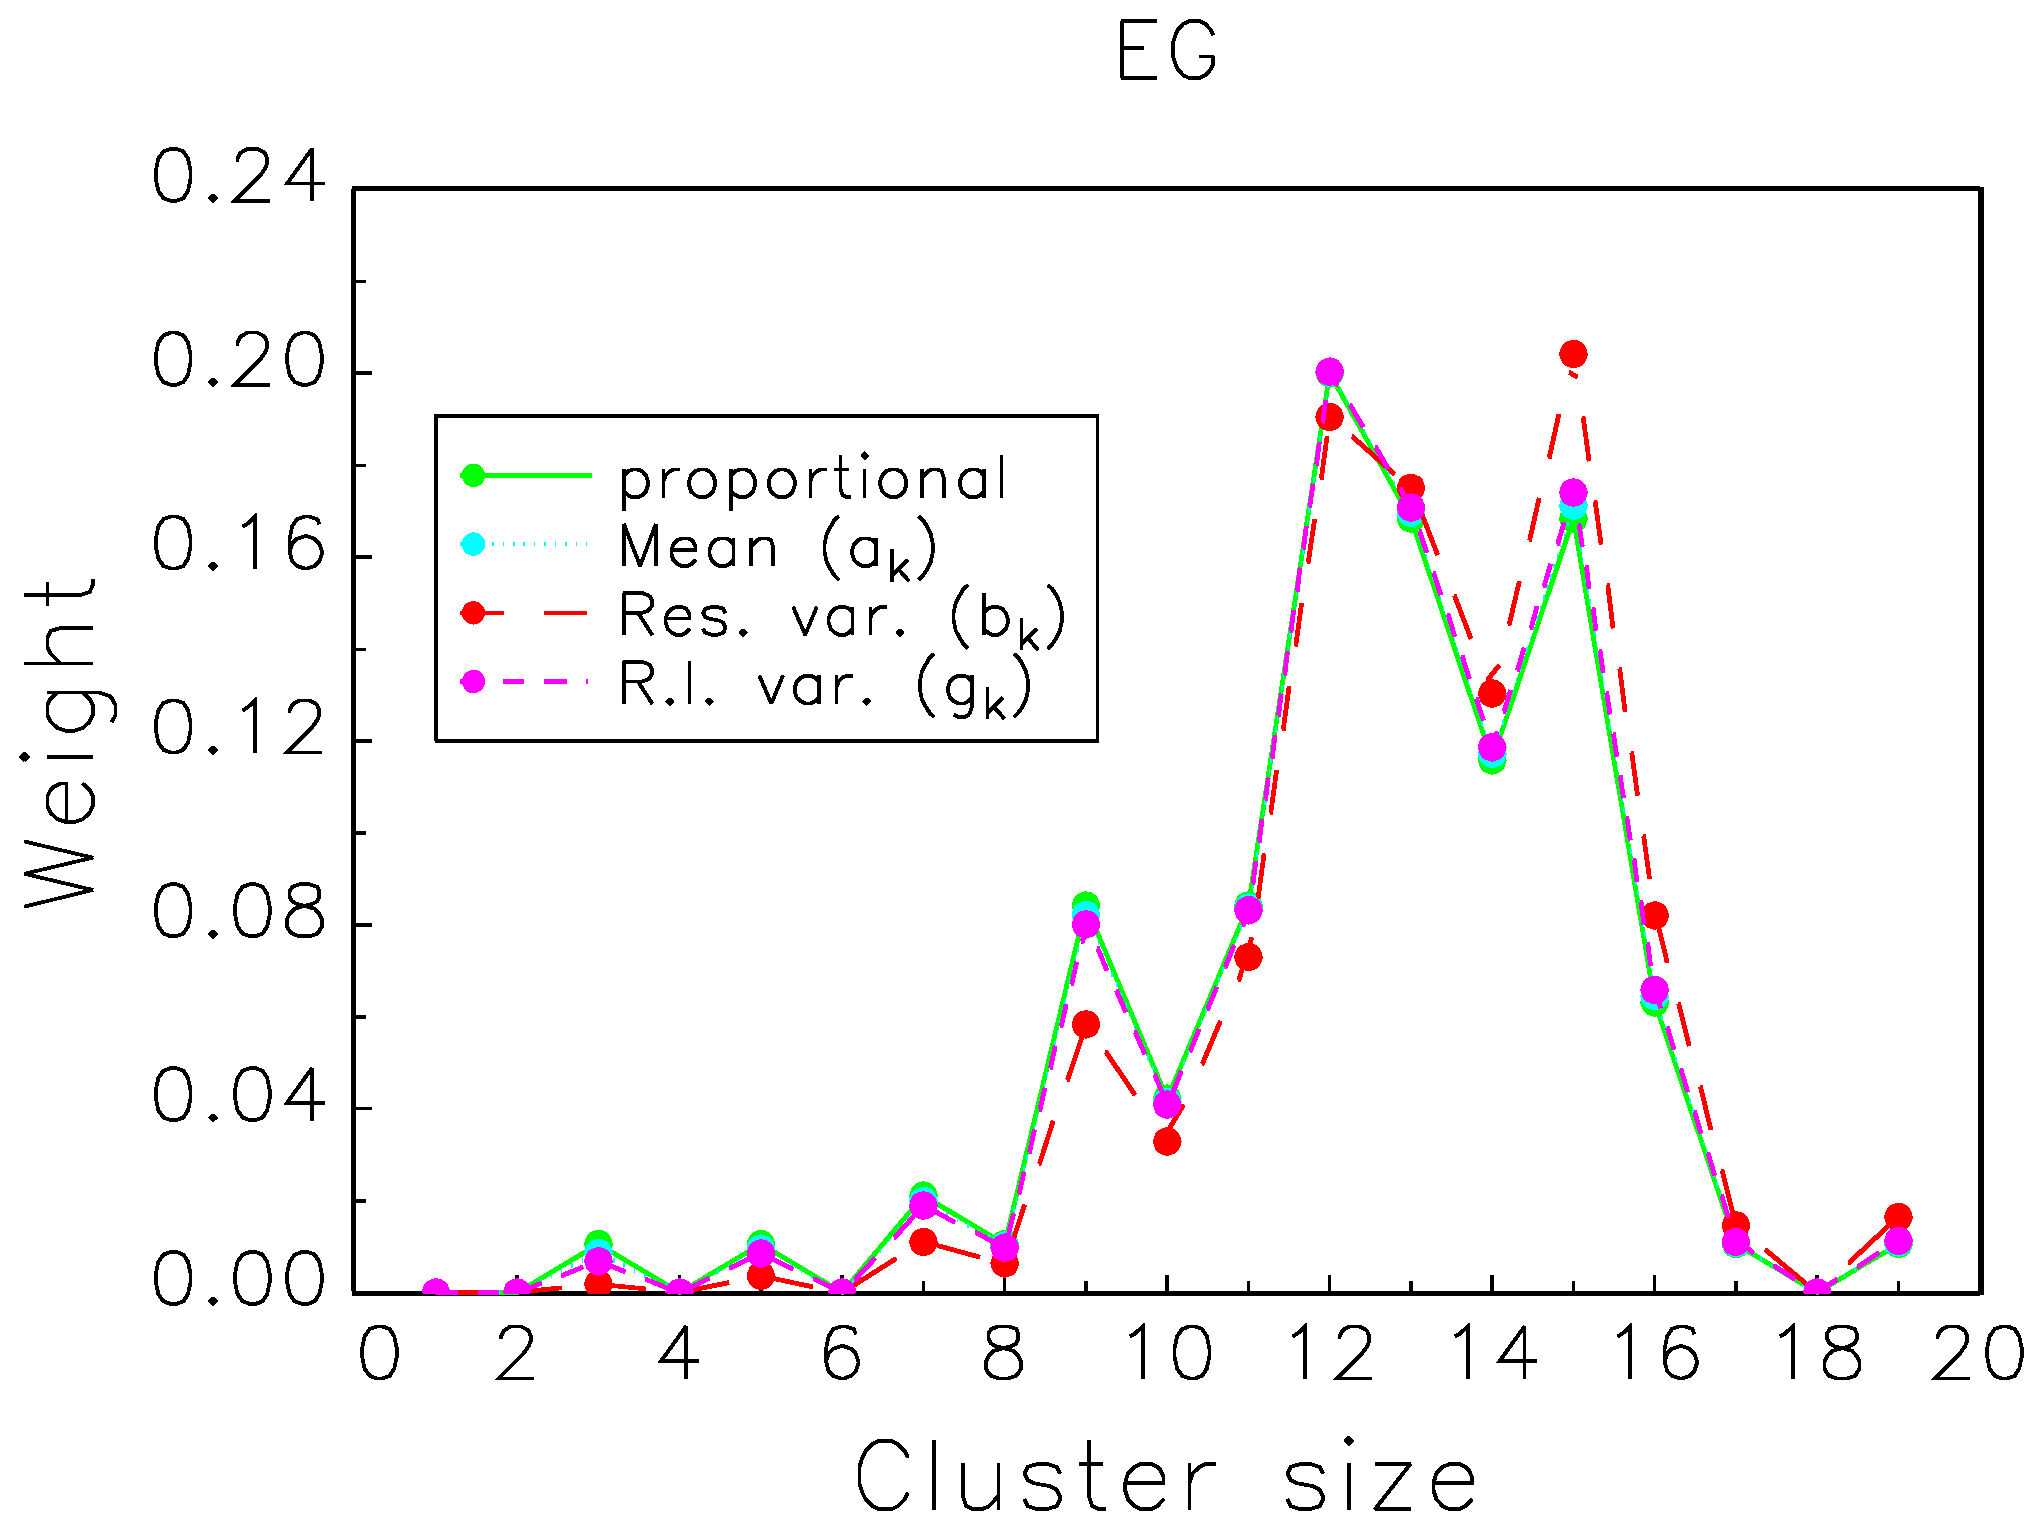
\includegraphics[width=7.5cm]{egclipped.eps}
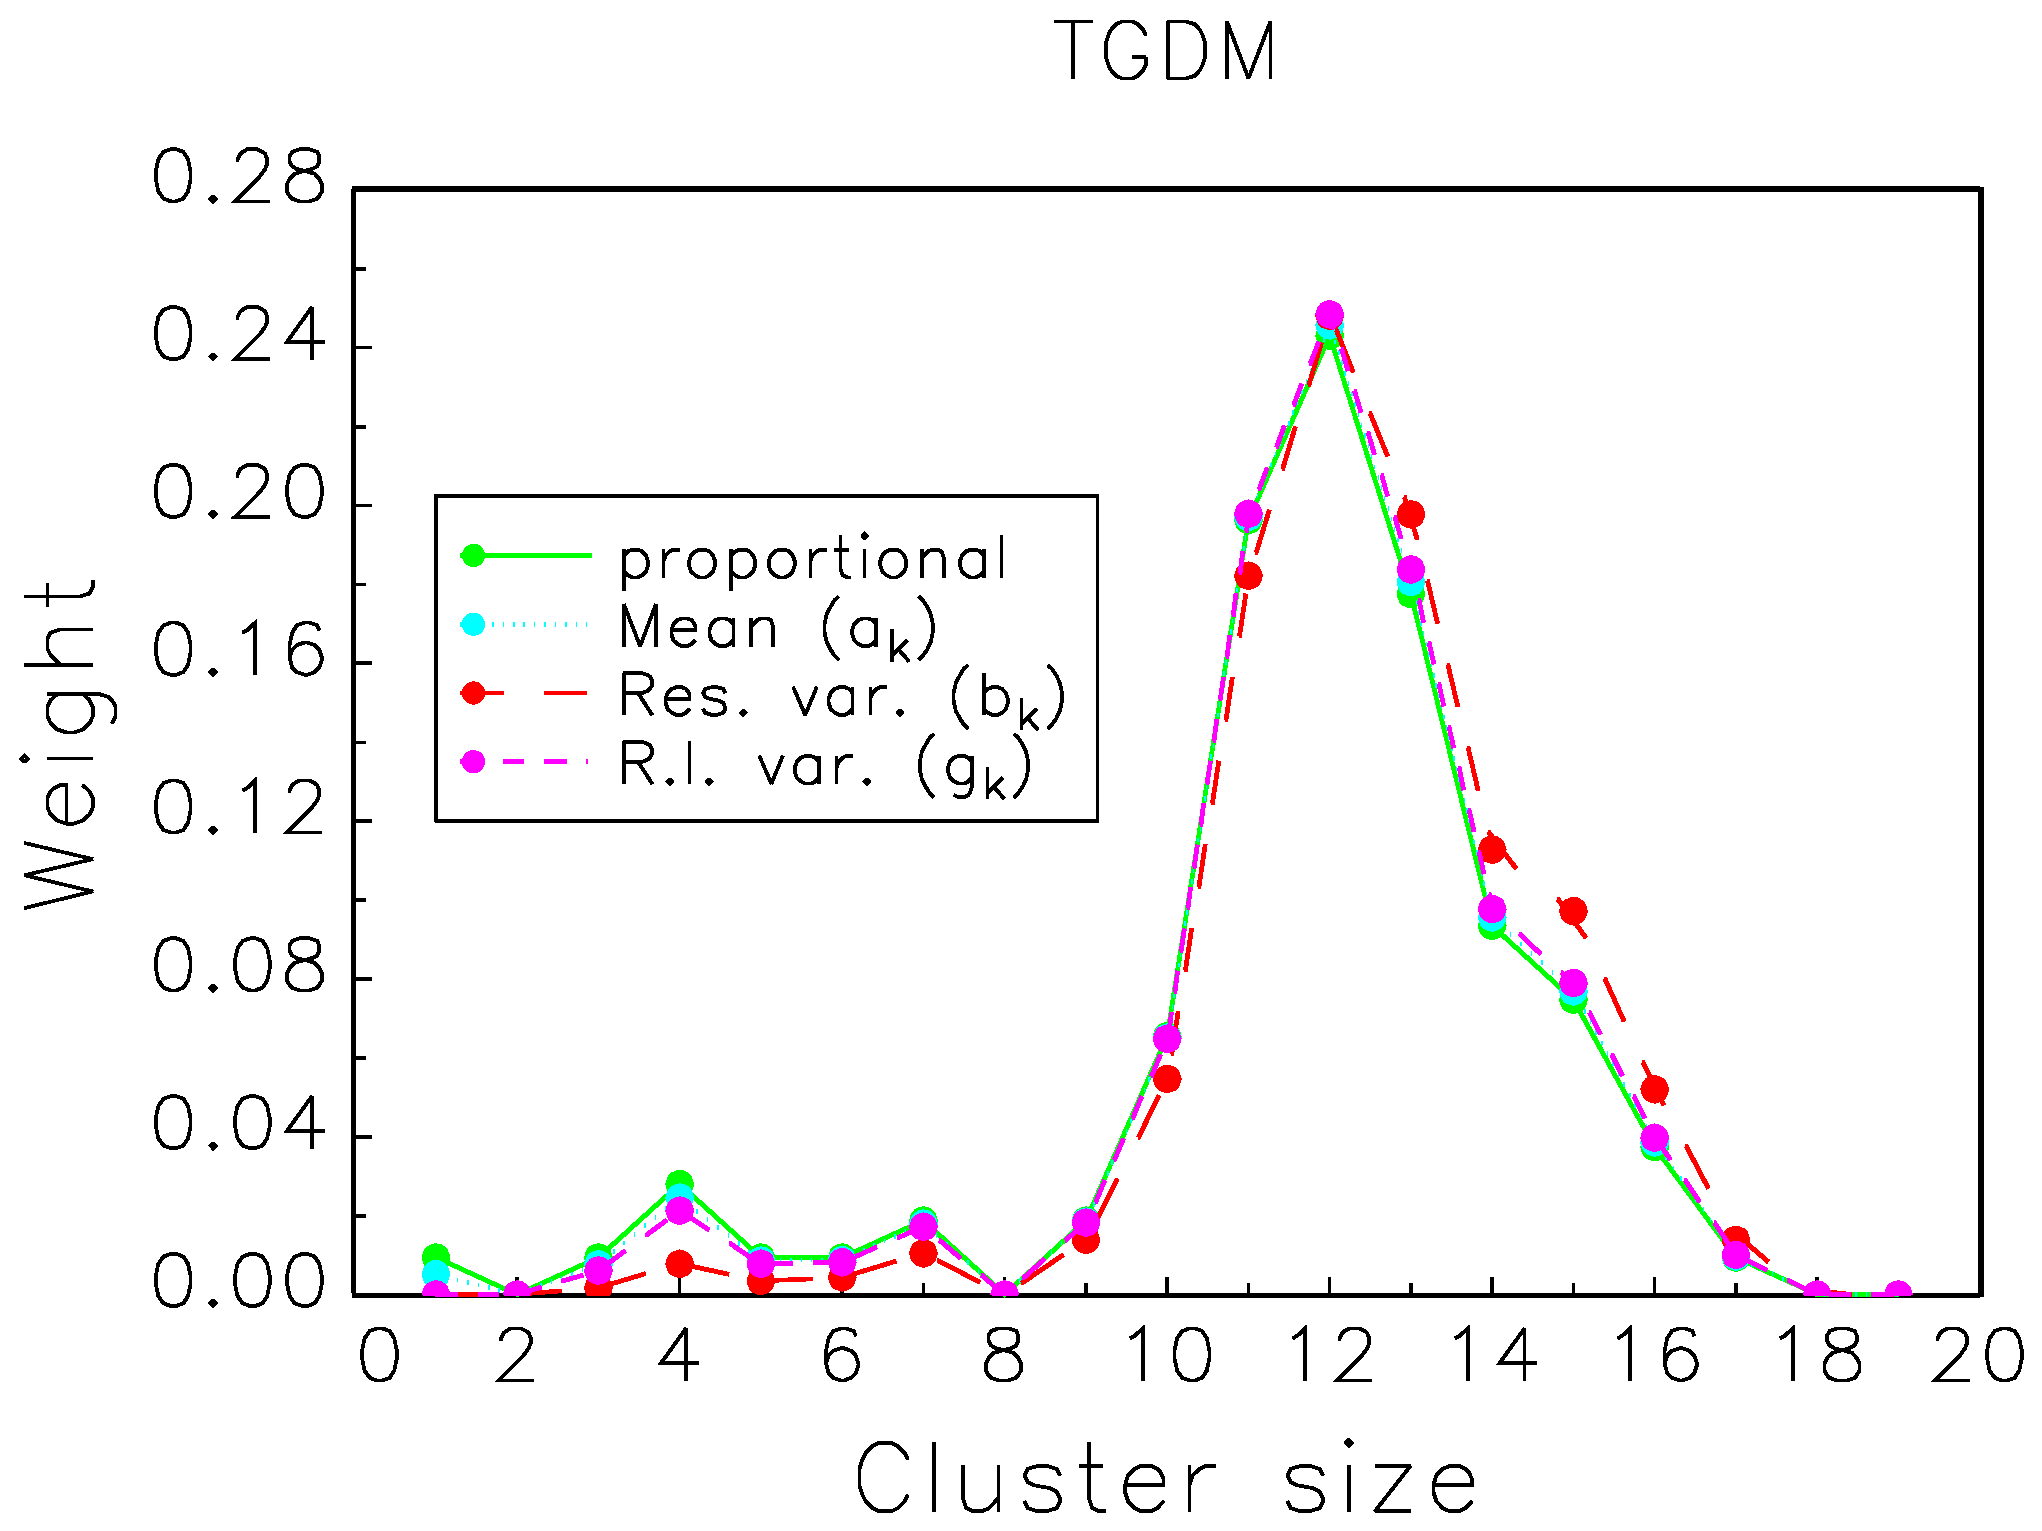
\includegraphics[width=7.5cm]{tgdmclipped.eps}
\caption{\small \linespread{1.1} NTP Data. Scalar weights: proportional and optimal scalar versions for EG and TGDM datasets. The optimal scalar weights are computed for $\rho=d/(\sigma^2+d)=0.5$.}
\label{ntpweightfigure}
\end{center}
\end{figure}
In both cases, there is a considerable range of cluster sizes, approximately 
1 to 20. At the same time, the frequencies of the cluster sizes vary 
considerably. The values for $a_k$ and $g_k$ are almost identical to 
the proportional weights. While a small discrepancy for $b_k$ is 
noticeable, and understandable in view of (\ref{bkapprox}), the 
proportional weights seem to offer a sensible choice. This issue 
will be examined further in the data-analytic Section~8.
%\ref{dataanal}.

\subsubsection{The Special Case of Common Cluster Size, Splits of (Un)equal Size}
\label{horizontal}

When $n_k\equiv n$ is constant, (\ref{akbasic})--(\ref{gkbasic}) reduce to:
\begin{equation}
\label{akbkgk}
a_k=b_k=g_k={c_k}/{N},
\end{equation}
Hence, while $a_k=b_k$ reduce to proportional weights,  for $g_k$ there is an impact of the partitioning structure. 
When, further, $c_k$ is constant, we obtain $a_k=b_k=g_k=c/N=1/K$,
and equal weights follow. The similarities and the subtle differences with the results from Section~6.1.4
%\ref{aow} 
are worth pointing out. Expressions (\ref{aoweq}) 
and (\ref{akbkgk}) are identical except for the parameter $\sigma^2$.

\subsubsection{Cluster-by-cluster Analysis}\label{cbca}

The expressions presented earlier in this section, using optimal weights 
and variations on this theme, can be applied when the partitioning is 
as extreme as possible: a single cluster per stratum. This sets $c_k\equiv 1$. Evidently, the $n_k$ will 
then no longer be unique, but that is immaterial; while we make use of the fact that the cluster size is  constant within a stratum, it does not need to be different 
between  strata. We examine this case in more detail in Supplementary Materials Section~S5.1.
%\ref{cbcaapp}. 
In particular, we derive under what asymptotics such an estimator is consistent. 



\subsection{Simulation Study}
\label{simulation}

A first, limited, simulation study was carried out to examine the behavior of the 
partitioning method. Details are given in Supplementary Materials Section~S6.
%\ref{simapp}. 
Three settings were considered: (1) $c_k\cdot n_k$ is kept constant with the factors taking different values; (2) $c_k$ is kept constant; (3) $n_k$ is kept constant. For all of these, $k$ goes from 1 to 4, so that there are four sub-samples. Apart from full likelihood, a series of weights was considered: equal, proportional  to $c_k$, size proportional to $c_k\cdot n_k$, approximate optimal, and iterated optimal.

From the results it is clear that equal weights are not a good choice. For $\mu$ and $d$,  proportional weights are excellent, while for $\sigma^2$ so are the size proportional weights. Iterated optimal weights perform considerably better than approximate optimal weights, in the sense  that the latter, like equal weights, arguably should not be considered  for practice. When comparing iterated and approximate optimal weights, 
the former are more computationally intensive.

However, iterated optimal weights give results very close to proportional 
weights (for $\mu$ and $d$) and to size proportional weights (for $\sigma^2$). 
Importantly, all of these results are very close to the ones 
obtained from maximum likelihood.

As a consequence, we have a simple, non-iterative set of weights at our 
disposal, free of unknown parameters, with excellent performance.

A second simulation study compares the proposed methods to two alternatives: full maximum likelihood and multiple imputation. Details are reported in Supplementary Materials Section~S7.
%\ref{simapptwee}. 
The most striking conclusion is that closed-form solutions are  much faster than their alternatives while, at the same time, yielding most precise results.
The time gain of our fastest method relative to standard maximum likelihood using PROC MIXED ranges from 5 times to 30,000 times faster.

{0} %-1
\subsection{Analysis of Case Study}
\label{dataanal}

The data, introduced in Section~2,
%\ref{ntpintro}, 
were analyzed in three ways. 
In Section~8.1
%\ref{basic} 
maximum likelihood estimators are presented, with split sampling, where splitting is by cluster size and using various weighting schemes. In Section~8.2,
%\ref{withdose}, 
a dose effect is added to these. Finally, the cluster-by-cluster methodology of Section~6.3
%\ref{cbca} 
is illustrated in Section~8.3.
%\ref{cbc}.

\subsubsection{Splitting by Cluster Size, No Dose Effect}
\label{basic}

Tables~\ref{ntpestimatestable4}--\ref{ntpestimatestable6} present (restricted) maximum likelihood estimates (standard errors), together with those from various weighted 
estimators. The standard CS model is fitted to the fetal 
weight outcome, ignoring the dose effect. Because there is an effect of 
dose on litter size, the mean is associated with cluster size. It is therefore 
interesting to assess the impact of this on the split-sample estimators, 
when compared to the MLEs. 
\begin{table}[t!]
\begin{center}
\caption[Cluster-by-cluster analysis- DEHP]{\linespread{1}\small NTP Data (DEHP). Cluster-by-cluster analysis. Maximum likelihood and weighted split-sample estimates (standard errors): (a) ML: maximum likelihood; (b) REML: restricted maximum likelihood; (c) Prop.: proportional weights; (d) Equal: equal weights; (e) Approx.~sc.: like proportional weights, except that for $b_k$ (\ref{bkapprox}) is used; (f) Scalar: scalar weights, with the sub-sample specific weights plugged in for the parameters figuring in the weights; (g) Opt.: optimal weights, with the sub-sample specific weights plugged in for the parameters figuring in the weights. Proper: proper variances for optimal weights \label{ntpestimatestable4}}


\vspace*{2mm}
\def\arraystretch{0.6}\small\tabcolsep=2truept \begin{tabular}{ccccccccc}
\hline\hline
     &   &     &      &             &         &      & \multicolumn{2}{c}{Optimal}\\
\cline{8-9}
 Par.& ML& REML& Prop.& Equal       & Approx.~sc.&Scalar& Simpl. & Proper\\
\hline
\hline
%\multicolumn{9}{c}{{Weighted [(\ref{muconstant})(\ref{sigmaconstant})(\ref{dconstant})]}}\\
\multicolumn{9}{c}{{Weighted [(S5.2)(S5.3)(S5.4)]}}\\
\hline
$\mu$ & 0.90718 & 0.90716 & 0.90602 & 0.89558 & 0.90602 & 0.92080 & \multicolumn{2}{c}{0.92080}   \\
$\sigma^2$ & 0.01877 & 0.01877 & 0.02122 & 0.02244 & 0.01895 & 0.01871 & \multicolumn{2}{c}{0.01246}  \\
$d$ & 0.01181 & 0.01195 & 0.00951 & 0.01016 & 0.00951 & 0.00085 & \multicolumn{2}{c}{0.00087}  \\
\hline
$\mbox{s.e.}(\widehat{\mu})$ & 0.01149 & 0.01155 & 0.01076 & 0.01360 & 0.01076 & 0.00766 & 0.00766 & 0.00766 \\
$\mbox{s.e.}(\widehat{\sigma^2})$ & 0.00084 & 0.00084 & 0.00128 & 0.00199 & 0.00094 & 0.00092 & 0.00061 & 0.00138 \\
  $\mbox{s.e.}(\widehat{d})$ & 0.00196 & 0.00199 & 0.00210 & 0.00293 & 0.00210 & 0.00048 & 0.00045 & 0.00340 \\
\hline\hline
%\multicolumn{9}{c}{{Two-stage [(\ref{muconstant})(\ref{twostages1})(\ref{twostaget1})]}}\\
\multicolumn{9}{c}{{Two-stage [(S5.2)(S5.7)(S5.8)]}}\\
\hline
$\mu$ & 0.90718 & 0.90716 & 0.90602 & 0.89558 & 0.90602 & 0.92119 & \multicolumn{2}{c}{0.92119}  \\
$\sigma^2$ & 0.01877 & 0.01877 & 0.01868 & 0.01931 & 0.01696 & 0.01679 & \multicolumn{2}{c}{0.01155}  \\
$d$ & 0.01181 & 0.01195 & 0.01204 & 0.01329 & 0.01204 & 0.00362 & \multicolumn{2}{c}{0.00376}  \\

\hline
$\mbox{s.e.}(\widehat{\mu})$ & 0.01149 & 0.01155 & 0.01169 & 0.01496 & 0.01169 & 0.00901 & 0.00901 & 0.00901 \\
$\mbox{s.e.}(\widehat{\sigma^2})$ & 0.00084 & 0.00084 & 0.00092 & 0.00127 & 0.00074 & 0.00072 & 0.00057 & 0.02404 \\
  $\mbox{s.e.}(\widehat{d})$& 0.00196 & 0.00199 & 0.03045 & 0.02915 & 0.03045 & 0.02537 & 0.00087 & 0.27337 \\

\hline\hline
%\multicolumn{9}{c}{{Unbiased two-stage [(\ref{muconstant})(\ref{twostages2})(\ref{twostaget2})]}}\\
\multicolumn{9}{c}{{Unbiased two-stage [(S5.2)(S5.11)(S5.12)]}}\\
\hline
$\mu$ & 0.90718 & 0.90716 & 0.90602 & 0.89558 & 0.90602 & 0.92195 & \multicolumn{2}{c}{0.92195}  \\
$\sigma^2$ & 0.01877 & 0.01877 & 0.02122 & 0.02244 & 0.01895 & 0.01871 & \multicolumn{2}{c}{0.01244}  \\
$d$ & 0.01181 & 0.01195 & 0.01390 & 0.01609 & 0.01390 & 0.00448 & \multicolumn{2}{c}{0.00467}  \\

\hline
$\mbox{s.e.}(\widehat{\mu})$& 0.01149 & 0.01155 & 0.01257 & 0.01679 & 0.01257 & 0.00958 & 0.00958 & 0.00958 \\
$\mbox{s.e.}(\widehat{\sigma^2})$  & 0.00084 & 0.00084 & 0.00128 & 0.00199 & 0.00094 & 0.00092 & 0.00061 & 0.00172 \\
  $\mbox{s.e.}(\widehat{d})$ & 0.00196 & 0.00199 & 0.00291 & 0.00447 & 0.00291 & 0.00101 & 0.00102 & 0.00634 \\

\hline\hline
\end{tabular}
\end{center}
\end{table}



%%%%%%%%%%%%%%%%%%%%%% EG



\begin{table}[!t]
\begin{center}
\caption[Cluster-by-cluster analysis, EG]{\linespread{1}\small  NTP Data (EG). Cluster-by-cluster analysis. Maximum likelihood and weighted split-sample estimates (standard errors): (a) ML: maximum likelihood; (b) REML: restricted maximum likelihood; (c) Prop.: proportional weights; (d) Equal: equal weights; (e) Approx.~sc.: like proportional weights, except that for $b_k$ (\ref{bkapprox}) is used; (f) Scalar: scalar weights, with the sub-sample specific weights plugged in for the parameters figuring in the weights; (g) Opt.: optimal weights, with the sub-sample specific weights plugged in for the parameters figuring in the weights. Proper: proper variances for optimal weights \label{ntpestimatestable5}}


\vspace*{2mm}

\def\arraystretch{0.6}\small\tabcolsep=2truept \begin{tabular}{ccccccccc}
\hline\hline
     &   &     &      &             &         &      & \multicolumn{2}{c}{Optimal}\\
\cline{8-9}
 Par.& ML& REML& Prop.& Equal       & Approx.~sc.&Scalar& Simpl. & Proper\\
\hline
\hline
%\multicolumn{9}{c}{{Weighted [(\ref{muconstant})(\ref{sigmaconstant})(\ref{dconstant})]}}\\
\multicolumn{9}{c}{{Weighted [(S5.2)(S5.3)(S5.4)]}}\\
\hline
$\mu$ & 0.82952 & 0.82952 & 0.83342 & 0.84653 & 0.83342 & 0.84133 & \multicolumn{2}{c}{0.84133}  \\
$\sigma^2$ & 0.00886 & 0.00886 & 0.00885 & 0.00899 & 0.00879 & 0.00878 & \multicolumn{2}{c}{0.00608}  \\
$d$ & 0.01704 & 0.01724 & 0.01606 & 0.01536 & 0.01606 & 0.01381 & \multicolumn{2}{c}{0.01408}  \\
\hline
$\mbox{s.e.}(\widehat{\mu})$ & 0.01402 & 0.01410 & 0.01393 & 0.01485 & 0.01393 & 0.01346 & 0.01346 & 0.01346 \\
$\mbox{s.e.}(\widehat{\sigma^2})$ & 0.00041 & 0.00041 & 0.00046 & 0.00051 & 0.00044 & 0.00044 & 0.00031 & 0.00328 \\
  $\mbox{s.e.}(\widehat{d})$& 0.00265 & 0.00269 & 0.00264 & 0.00272 & 0.00264 & 0.00230 & 0.00230 & 0.00476 \\
\hline\hline
%\multicolumn{9}{c}{{Two-stage [(\ref{muconstant})(\ref{twostages1})(\ref{twostaget1})]}}\\
\multicolumn{9}{c}{{Two-stage [(S5.2)(S5.7)(S5.8)]}}\\
\hline
$\mu$ & 0.82952 & 0.82952 & 0.83342 & 0.84653 & 0.83342 & 0.84100 & \multicolumn{2}{c}{0.84100}   \\
$\sigma^2$ & 0.00886 & 0.00886 & 0.00803 & 0.00814 & 0.00802 & 0.00802 & \multicolumn{2}{c}{0.00559}  \\
$d$& 0.01704 & 0.01724 & 0.01688 & 0.01621 & 0.01688 & 0.01476 & \multicolumn{2}{c}{0.01499}  \\

\hline
$\mbox{s.e.}(\widehat{\mu})$ & 0.01402 & 0.01410 & 0.01423 & 0.01522 & 0.01423 & 0.01379 & 0.01379 & 0.01379 \\
$\mbox{s.e.}(\widehat{\sigma^2})$ & 0.00041 & 0.00041 & 0.00037 & 0.00041 & 0.00037 & 0.00037 & 0.00029 & 0.03410 \\
  $\mbox{s.e.}(\widehat{d})$ & 0.00265 & 0.00269 & 0.02814 & 0.02555 & 0.02814 & 0.02632 & 0.00243 & 0.05214 \\


\hline\hline
%\multicolumn{9}{c}{{Unbiased two-stage [(\ref{muconstant})(\ref{twostages2})(\ref{twostaget2})]}}\\
\multicolumn{9}{c}{{Unbiased two-stage [(S5.2)(S5.11)(S5.12)]}}\\
\hline
$\mu$  & 0.82952 & 0.82952 & 0.83342 & 0.84653 & 0.83342 & 0.83911 & \multicolumn{2}{c}{0.83911}  \\
$\sigma^2$ & 0.00886 & 0.00886 & 0.00885 & 0.00899 & 0.00879 & 0.00878 & \multicolumn{2}{c}{0.00608}  \\
$d$ & 0.01704 & 0.01724 & 0.01857 & 0.01833 & 0.01857 & 0.01657 & \multicolumn{2}{c}{0.01684}  \\

\hline
$\mbox{s.e.}(\widehat{\mu})$ & 0.01402 & 0.01410 & 0.01493 & 0.01665 & 0.01493 & 0.01452 & 0.01452 & 0.01452 \\
$\mbox{s.e.}(\widehat{\sigma^2})$ & 0.00041 & 0.00041 & 0.00046 & 0.00051 & 0.00044 & 0.00044 & 0.00031 & 0.00363 \\
  $\mbox{s.e.}(\widehat{d})$ & 0.00265 & 0.00269 & 0.00302 & 0.00333 & 0.00302 & 0.00271 & 0.00271 & 0.00533 \\


\hline\hline
\end{tabular}
\end{center}
\end{table}



%%%%%%%%%%%%%%%%%%%%%% DYME



\begin{table}[!t]
\begin{center}
\caption[Cluster-by-cluster analysis, DYME]{ \linespread{1}\small NTP Data (DYME). Cluster-by-cluster analysis. Maximum likelihood and weighted split-sample estimates (standard errors): (a) ML: maximum likelihood; (b) REML: restricted maximum likelihood; (c) Prop.: proportional weights; (d) Equal: equal weights; (e) Approx.~sc.: like proportional weights, except that for $b_k$ (\ref{bkapprox}) is used; (f) Scalar: scalar weights, with the sub-sample specific weights plugged in for the parameters figuring in the weights; (g) Opt.: optimal weights, with the sub-sample specific weights plugged in for the parameters figuring in the weights. Proper: proper variances for optimal weights \label{ntpestimatestable6}}


\vspace*{2mm}

\def\arraystretch{0.6}\small\tabcolsep=2truept \begin{tabular}{ccccccccc}
\hline\hline
     &   &     &      &             &         &      & \multicolumn{2}{c}{Optimal}\\
\cline{8-9}
 Par.& ML& REML& Prop.& Equal       & Approx.~sc.&Scalar& Simpl. & Proper\\
\hline
\hline
%\multicolumn{9}{c}{{Weighted [(\ref{muconstant})(\ref{sigmaconstant})(\ref{dconstant})]}}\\
\multicolumn{9}{c}{{Weighted [(S5.2)(S5.3)(S5.4)]}}\\
\hline
$\mu$ & 0.84142 & 0.84141 & 0.84108 & 0.84861 & 0.84108 & 0.90166 & \multicolumn{2}{c}{0.90166}  \\
$\sigma^2$ & 0.01031 & 0.01031 & 0.01072 & 0.01071 & 0.01034 & 0.01031 & \multicolumn{2}{c}{0.00700}  \\
$d$ & 0.03657 & 0.03695 & 0.03102 & 0.03445 & 0.03102 & 0.00745 & \multicolumn{2}{c}{0.00755}  \\
\hline
$\mbox{s.e.}(\widehat{\mu})$ & 0.01926 & 0.01936 & 0.01780 & 0.02502 & 0.01780 & 0.01257 & 0.01257 & 0.01257 \\
$\mbox{s.e.}(\widehat{\sigma^2})$ & 0.00044 & 0.00044 & 0.00052 & 0.00079 & 0.00047 & 0.00046 & 0.00033 & 0.00308 \\
  $\mbox{s.e.}(\widehat{d})$ & 0.00529 & 0.00537 & 0.00570 & 0.01043 & 0.00570 & 0.00159 & 0.00159 & 0.00329 \\
\hline
\hline
%\multicolumn{9}{c}{{Two-stage [(\ref{muconstant})(\ref{twostages1})(\ref{twostaget1})]}}\\
\multicolumn{9}{c}{{Two-stage [(S5.2)(S5.7)(S5.8)]}}\\
\hline
$\mu$ & 0.84142 & 0.84141 & 0.84108 & 0.84861 & 0.84108 & 0.90009 & \multicolumn{2}{c}{0.90009}  \\
  $\sigma^2$ & 0.01031 & 0.01031 & 0.00975 & 0.00964 & 0.00945 & 0.00942 & \multicolumn{2}{c}{0.00650}  \\
$d$ & 0.03657 & 0.03695 & 0.03199 & 0.03552 & 0.03199 & 0.00836 & \multicolumn{2}{c}{0.00845}  \\

\hline
$\mbox{s.e.}(\widehat{\mu})$ & 0.01926 & 0.01936 & 0.01804 & 0.02535 & 0.01804 & 0.01297 & 0.01297 & 0.01297 \\
$\mbox{s.e.}(\widehat{\sigma^2})$ & 0.00044 & 0.00044 & 0.00042 & 0.00059 & 0.00039 & 0.00039 & 0.00030 & 0.02568 \\
  $\mbox{s.e.}(\widehat{d})$ & 0.00529 & 0.00537 & 0.03433 & 0.03113 & 0.03433 & 0.02215 & 0.00173 & 0.04036 \\
\hline\hline
%\multicolumn{9}{c}{{Unbiased two-stage [(\ref{muconstant})(\ref{twostages2})(\ref{twostaget2})]}}\\
\multicolumn{9}{c}{{Unbiased two-stage [(S5.2)(S5.11)(S5.12)]}}\\
\hline
$\mu$ & 0.84142 & 0.84141 & 0.84108 & 0.84861 & 0.84108 & 0.89672 & \multicolumn{2}{c}{0.89672}  \\
  $\sigma^2$ & 0.01031 & 0.01031 & 0.01072 & 0.01071 & 0.01034 & 0.01031 & \multicolumn{2}{c}{0.00700}  \\
$d$  & 0.03657 & 0.03695 & 0.03690 & 0.04514 & 0.03690 & 0.01027 & \multicolumn{2}{c}{0.01037}  \\

\hline
$\mbox{s.e.}(\widehat{\mu})$ & 0.01926 & 0.01936 & 0.01937 & 0.02989 & 0.01937 & 0.01390 & 0.01390 & 0.01390 \\
$\mbox{s.e.}(\widehat{\sigma^2})$ & 0.00044 & 0.00044 & 0.00052 & 0.00079 & 0.00047 & 0.00046 & 0.00033 & 0.00353 \\
  $\mbox{s.e.}(\widehat{d})$ & 0.00529 & 0.00537 & 0.00718 & 0.01542 & 0.00718 & 0.00205 & 0.00205 & 0.00382 \\

\hline\hline
\end{tabular}
\end{center}
\end{table}


The ML and REML are very similar, with equal point estimates for $\mu$, 
nearly equal estimates for $\sigma^2$, and similar estimates for $d$. 
The equality for the mean estimator is known for the CS case. 
The difference in the estimates of $\sigma^2$ arises because 
the denominator used in its calculation is, for ML, the total number of 
fetuses and, for REML, the same figure less one.
For $d$, the difference is in terms of the cluster sizes 
(division by $n_i$ or $n_i-1$), which is more noticeable. 
All weighted estimators, except with equal weights, 
lead to very similar point estimates; this is in line with the 
simulation results. Even for equal weights, the difference 
is not worrisome. Proportional, equal, and approximate scalar 
weights are parameter-free and depend at most on the cluster 
size and/or the number of clusters per size. This explains 
why these estimators yield standard errors similar to the 
likelihood-based ones. Not surprisingly, because of their 
deviation from optimality, equal weights lead to increased 
uncertainty.

For the scalar and optimal estimators two issues need to be 
borne in mind. First, in principle they require knowledge of 
the true parameters. In the absence of them, plug-in estimates 
were used. Because of the independence between mean and 
variance parameters, both methods produce the same results 
for $\mu$. Also, the estimates for $\mu$ are similar to the 
likelihood-based ones. For $\sigma^2$, this scalar-weight 
method works better than the optimal, matrix-based one. 
Because 
of their matrix nature, optimal weights are less stable when approximated. 
The standard errors are underestimated because uncertainty, 
stemming from plugging in the weights is ignored when 
using the `simplified' precision estimates. When rectified 
(`proper' weights), there is no difference for the mean parameter, 
because the weights are parameter-free, but there is a strong 
difference for the variance components. Once the proper standard 
errors are calculated, it is clear that there is information 
loss because of using plug-in estimates in the weights, 
rather than the true ones.

\subsubsection{Splitting by Cluster Size, With Dose Effect}
\label{withdose}

While these results illustrate the explicit derivations  with a constant mean, the data analysis in Section~8.1
%\ref{basic} 
does not do full justice to the actual design of the experiment, because the question of  scientific interest is the 
dose-response relationship. Let $x_i$ be the dose administered to 
cluster $i$, taking one out of 4 to 5 values. The dose 
levels for the DEHP study are given in Table~\ref{tabclus}. The model 
then is $\BY_i\sim N\left(\left\{\beta_0+\beta_1x_i\right\}\mathbf{1}_n,\sigma^2 I_{n}+d J_{n}\right)$. 
Because the mean and covariance parameters are functionally and 
statistically independent within a sub-sample of constant cluster size, 
the considerations presented for the constant-mean case will remain valid. 
The results of fitting this extended model to the DEHP, EG, and DYME compounds, 
under ML (and REML) on the one hand, and using split-sample methodology 
(with proportional, equal, and approximate scalar weights) on the other, 
are presented in Table~\ref{ntpestimatestable3}. The results are  
comforting, showing that proportional and approximate scalar weights are a sensible choice. This is consistent with theoretical considerations, 
the simulations results, and the analysis in Section~8.1.
%\ref{basic}.
\begin{table}[!t]
\begin{center}
\caption[NTP Data (with dose effect)]{\linespread{1} \small NTP Data (with dose effect). Splitting by cluster size.  Maximum likelihood and weighted split-sample estimates (standard errors): (a) ML: maximum likelihood; (b) REML: restricted maximum likelihood; (c) Prop.: proportional weights; (d) Equal: equal weights; (e) Approx.~sc.: like proportional weights, except that for $b_k$ (\ref{bkapprox}) is used.\label{ntpestimatestable3}}


\vspace*{2mm}
\def\arraystretch{0.55}\small\tabcolsep=3truept \begin{tabular}{lrrrrr}
\hline\hline
 Par.& \multicolumn{1}{c}{ML}& \multicolumn{1}{c}{REML}& \multicolumn{1}{c}{Prop.}& \multicolumn{1}{c}{Equal}       & \multicolumn{1}{c}{Approx.~sc.}\\
\hline
\hline
\multicolumn{6}{c}{{DEHP}}\\
\hline
Interc.\ $\beta_0$ & 0.96986 & 0.96987 & 0.95982 & 0.95269 & 0.95982 \\
  Dose eff.\ $\beta_1$ & -0.00077 & -0.00077 & -0.00042 & -0.00029 & -0.00042 \\
 $\sigma^2$ & 0.01876 & 0.01876 & 0.02122 & 0.02244 & 0.01895 \\
  $d$& 0.00772 & 0.00792 & 0.00538 & 0.00508 & 0.00538 \\
\hline
s.e.($\widehat{\beta_0}$) & 0.01343 & 0.01357 & 0.01343 & 0.01609 & 0.01343 \\
s.e.($\widehat{\beta_1}$) & 0.00012 & 0.00012 & 0.00014 & 0.00018 & 0.00014 \\
s.e.($\widehat{\sigma^2}$) & 0.00084 & 0.00084 & 0.00128 & 0.00199 & 0.00094 \\
s.e.($\widehat{d}$) & 0.00136 & 0.00141 & 0.00137 & 0.00204 & 0.00137 \\
\hline\hline
\multicolumn{6}{c}{{EG}}\\
\hline
Interc.\ $\beta_0$& 0.94228 & 0.94229 & 0.94654 & 0.95320 & 0.94654 \\
 Dose eff.\ $\beta_1$ & -0.00009 & -0.00009 & -0.00010 & -0.00010 & -0.00010 \\
 $\sigma^2$ & 0.00879 & 0.00879 & 0.00847 & 0.00847 & 0.00833 \\
$d$ & 0.00745 & 0.00765 & 0.00625 & 0.00593 & 0.00625 \\
\hline
s.e.($\widehat{\beta_0}$) & 0.01453 & 0.01470 & 0.01389 & 0.01406 & 0.01389 \\
s.e.($\widehat{\beta_1}$) & 0.00001 & 0.00001 & 0.00001 & 0.00001 & 0.00001 \\
 s.e.($\widehat{\sigma^2}$) & 0.00041 & 0.00041 & 0.00044 & 0.00049 & 0.00042 \\
 s.e.($\widehat{d}$) & 0.00126 & 0.00130 & 0.00108 & 0.00107 & 0.00108 \\
\hline\hline
\multicolumn{6}{c}{{DYME}}\\
\hline
Interc.\ $\beta_0$& 1.01875 & 1.01876 & 1.02364 & 1.03680 & 1.02364 \\
 Dose eff.\ $\beta_1$ & -0.00102 & -0.00102 & -0.00099 & -0.00100 & -0.00099 \\
 $\sigma^2$ & 0.01032 & 0.01032 & 0.01072 & 0.01071 & 0.01034 \\
$d$ & 0.00795 & 0.00813 & 0.00581 & 0.00631 & 0.00581 \\
\hline
s.e.($\widehat{\beta_0}$) & 0.01356 & 0.01370 & 0.01335 & 0.02000 & 0.01335 \\
s.e.($\widehat{\beta_1}$) & 0.00006 & 0.00006 & 0.00006 & 0.00007 & 0.00006 \\
s.e.($\widehat{\sigma^2}$) & 0.00044 & 0.00044 & 0.00052 & 0.00079 & 0.00047 \\
 s.e.($\widehat{d}$) & 0.00126 & 0.00130 & 0.00110 & 0.00205 & 0.00110 \\
\hline\hline
\end{tabular}
\end{center}
\end{table}

\subsubsection{Cluster-by-cluster Methods}
\label{cbc}

We illustrate the cluster-by-cluster methods here. Results are 
presented in Tables~\ref{ntpestimatestable4}--\ref{ntpestimatestable6}, 
for DEHP, EG, and DYME, respectively. For brevity, attention here is 
confined to the case of no dose effect.

We consider three alternatives. In all three, (S5.2)
%(\ref{muconstant}) 
is used for the mean. For the variance components, 
the pairs (S5.3)-(S5.4), (S5.7)-(S5.8), and (S5.11)-(S5.12)
%(\ref{sigmaconstant})--(\ref{dconstant}),
%(\ref{twostages1})--(\ref{twostaget1}), and 
%(\ref{twostages2})--(\ref{twostaget2}) 
are used, respectively. Because 
these expressions are derived for a given cluster size, 
we need to supplement them with a weighting method. For comparison, the 
same choices are made as reported in Tables~\ref{ntpestimatestable4}--\ref{ntpestimatestable6}.

Even though the same estimator {\em per cluster size\/} is used for 
the mean in all three cases, the overall result is different for scalar 
and optimal weights because these depend on the estimated variance 
components. A relatively clear message is that proportional and approximate 
scalar weights show very good performance. This is pleasing, because these 
weights are parameter-free and hence easy to apply. As to which of the three 
versions is better is less clear, this differs somewhat from compound to 
compound and from parameter to parameter. All three show 
acceptable behavior. It is interesting to see that in some cases the 
cluster-by-cluster analysis is closer to ML than the analyses based 
on splitting per cluster size. Computationally, this approach allows 
for additional parallel processing, with all clusters analyzed in parallel 
and the results then combined.


\subsection{Ramifications and Concluding Remarks}
\label{ramifications}

We considered the simple but insightful case of clustered data 
with a normal compound-symmetry structure and clusters of varying size. 
Here, there is no closed-form maximum 
likelihood estimator and maximization must proceed iteratively. Moreover, there is no uniform optimal unbiased estimator and the MLE is only locally optimal. 

When considering the collection of estimators 
obtained from analyzing the data for each cluster size separately, 
the MLE for the entire dataset is a vector linear combination of them, 
with the weights depending on the parameters.  Based 
on theoretical results and simulations, as well as on data analysis, 
we found that equal weights and so-called approximately optimal weights do 
not perform well. Iterated optimal and proportional weights show excellent 
performance, and they are simple and parameter-free. One refinement is 
that for the mean parameter and for the covariance term $d$ weights should 
be chosen proportional to the number of clusters of a particular size, 
$c_k$, while for the measurement error variance $\sigma^2$ proportionality 
is to the product of the number of clusters of a given size and the cluster 
size, $c_k\cdot n_k$.

While most of our development is based on the simple, three-parameter 
compound-symmetry model, in the data analysis we considered a slightly 
expanded setting, in which the mean takes the form of a regression 
function. This suggests the 
use of our results in more elaborate settings, as long as some 
form of exchangeability prevails. One such setting is the meta-analytic 
evaluation of surrogate endpoints \citep{burzykowski2006evaluation}, where two correlated 
endpoints rather than a single one are considered for each cluster 
(trial in this case). Admittedly, there may come a point where 
distinguishing between parameters where it is difficult to determine whether proportional weights or 
size proportional weights are to be preferred. Based on our simulation results, it may 
then be sensible to consider proportional weights for all parameters. 
In the case where clusters take the form of trials, the number of 
trials may be relatively small, and likely trial sizes are (almost) 
unique. Our split-sample method  then implies that each trial is 
first analyzed separately, with overall estimates taking the form of 
linear combinations of trial-specific ones. To provide a formal basis 
for this, we considered the important special case of a 
cluster-by-cluster analysis. Such a method is 
consistent when the number of replicates per cluster (e.g., 
the number of patients per trial) increases more rapidly than 
the number of trials.  Such an assumption is not realistic in
the developmental toxicology setting considered in this paper, 
but may be  sensible in a meta-analysis of clinical trials.

When clusters are very large, it may be attractive to further 
sub-divide them in sub-clusters. Such a splitting method was also 
considered by \cite{Iddi2011}. Its use in our context would require 
further investigation.

In the NTP data, the observed cluster size is related to the dose 
applied. This suggests that it is useful to consider, at the same 
time, the impact of dose on the outcomes (e.g., fetal weight) as 
well as on cluster size. This brings us back to the informative 
cluster sizes mentioned in the Introduction. While work has been 
done in this area, it is of interest to combine the ideas developed 
in this paper with a model for cluster size.





\newpage


\section[AR1 structure]{Fast, closed-form, and efficient estimators for hierarchical models with AR (1) covariance and unequal cluster sizes}

\label{sec_ar1}

\subsection{Introduction}
\label{secintroar1}

It is common for the number of study units in a design, the sample size, to be fixed {\em a priori\/}. However,
there are many exceptions to this. \cite{molenberghs2014random} provides an overview of such designs. Some examples are sequential trials, for which the sample size is determined by a stopping rule, missing data, and censored time-to-event data.
The focus of this paper is hierarchical data where independent replicates take the form of compound units, generically termed {\em clusters}.  Clustering can occur in many settings, for example, longitudinal data, toxicology \citep{aerts2002}, cluster randomized trials and, more generally, multi-level designs. The sizes of the resulting clusters can be fixed by design, or may be random. Random sample sizes can be due to missingness in the data, governed by a stochastic mechanism. And, in some cases, the cluster sizes may be associated with the outcomes, often termed `informative cluster sizes', see for example \cite{williamson2003marginal, benhin2005mean, hoffman2001, cong2007marginal, chiang2008efficient, wang2011inference,aerts2011incomplete}. However, our interest here is not on informative cluster sizes, but rather unequal cluster sizes that are themselves independent of observed and unobserved outcomes. We concentrate solely on the non-constant nature of the cluster sizes, for which joint modelling of outcomes and cluster size is not required.

\cite{hermans2017_cs} considered the setting of normally distributed clustered data with a compound-symmetry (CS) structure for the dependency, that is, a three-parameter multivariate normal model with a common mean $\mu$, a common variance $\sigma^2+d$, and a common covariance $d$. \cite{Lisa2015_2} showed that, unless the clusters are of the same size, the sufficient statistics are incomplete and the maximum likelihood estimators (MLEs) do not have closed-form solutions. By contrast, if the clusters are all the same size, and hence also within a subset of clusters of the same size, a closed form solution does exist for the MLEs: sufficient statistics are complete and the estimators are minimum variance unbiased. \cite{Iddi2011} studied the CS case and proposed a pseudo-likelihood split-sample approach, as follows. The original sample is divided into subsamples. Maximum likelihood estimation is separately applied to each subsample and the resulting subsample-specific estimators are averaged using appropriate weights. Appropriate measures of precision for the combined estimators are then obtained. In the current setting it is natural, with this approach, to define the subsamples according to the cluster size \citep{hermans2017_cs}. When the number of clusters and/or the cluster sizes are very large, standard iterative MLE computation times can become prohibitive. By contrast, the non-iterative nature of the split sample approach can lead to much lower computation times. For the CS setting, \cite{hermans2017_cs} show that
weights proportional to the cluster sizes perform very well for combining the individual estimators.

Although the CS covariance structure is a natural model for settings that exhibit within-cluster symmetry, other settings, such as longitudinal designs, need to be handled. For these we might consider the first-order autoregressive, AR(1), structure, where it is assumed that the correlation between two measurements changes exponentially over time, that is, $\sigma_{ij}=\sigma^2 \rho^{|i-j|}$. This implies that the variance of the measurements is a constant $\sigma^2$ and the covariance decreases with increasing time lag. In this paper, we apply the split-sample method to the normal AR(1)-model, which has three parameters, a common mean $\mu$, a common variance $\sigma^2$, and correlation parameter $\rho$. An important question will be the appropriate choice of weights in such a setting.

As a motivating example, we consider five clinical trials in\label{secmotex} schizophrenia.
These data were collected from five double-blind randomized clinical trials to compare the effects of two treatments
for chronic schizophrenia: risperidone and conventional antipsychotic agents. Subjects who received doses of risperidone (4--6~mg/day) or an active control (haloperidol, perphenazine, zuclopenthixol) have been included in the analysis.

Patients were clustered within country, and longitudinal measurements were made on each subject over time. The number of patients ranges from 9 tot 128 per country with a total of 2039.  The positive and negative syndrome scale (PANSS) was used to asses the global condition of a patient. This scale is constructed from 30 items, each taking values between 1 and 7, giving an overall range of 30 to 210. PANSS provides an operationalized, drug-sensitive instrument, which is useful for both typological and dimensional assessment of schizophrenia. Depending on the trial, treatment was administered for a duration of 48 weeks with at most 12 monthly measurements. Because not all subjects received treatment at the same time points and, not the same amount, the final dataset is unbalanced.

This dataset was also analyzed from a surrogate markers point perspective in \cite{alonso2004validation}. The focus here is on the treatment effect, accommodating the longitudinal nature of the response.

The rest of paper is organised as follows. In Section~\ref{secmodel} the model formulation is given. In Section~\ref{secestimators} the estimators for a single constant cluster size are presented. The (in)completeness property is outlined in Section~\ref{secincomplete}, and in Section~\ref{secvariable} various weighting schemes for clusters of unequal size are explored. In Section~\ref{seccompu}, a simulation study is described for the investigation of the performance of the suggested weights and the data are analysed in Section~\ref{secapp}. The closing discussion is presented in Section~\ref{secconcl}. Some additional background material is available in a separate, web-based appendix\footnote{Available at https://ibiostat.be/online-resources.}.

\subsection{Model Formulation}
\label{secmodel}

Suppose that there is a sample of $N$ independent clusters, among which $K$ different cluster sizes $n_{k}$ ($k=1,\dots,K$) can be distinguished. Let the multiplicity of cluster size $n_k$ be $c_k$. The total number of clusters is then $N=\sum_{k=1}^Kc_k$. Denote the outcome vector for the $i$th  ($i=1,\dots,c_k$) replicate among the clusters of size $n_k$ by $\BY_i^{(k)}$.

All models considered in this paper will be versions of the following general linear mixed model:
\begin{eqnarray}
\BY_i^{(k)}|\mathbf{b}_i^{(k)}&\sim&N(X_i^{(k)}\mathbf{\beta}+Z_i^{(k)}\mathbf{b}_i^{(k)},\Sigma_i^{(k)}),\label{lmmhier}\\[2mm]
\mathbf{b}_i^{(k)}&\sim&N(0,D),\label{lmmprior}
\end{eqnarray}
where $\bfbeta$ is a vector of fixed effects, and $X_i^{(k)}$ and $Z_i^{(k)}$ are design matrices. In what follows, we consider an AR(1) covariance structure, in which case
the term $\Zik\mathbf{b}_i^{(k)}$ drops\label{ar1firsttime} from (\ref{lmmhier}), while $\Sigma_i^{(k)}=\sigma^2C_{n_k}$, with entry $(r,s)$ equal to $\rho^{|r-s|}$. For ease of exposition, the mean structure will often be taken to be $\mu\mathbf{1}_{n_k}$, with $\mathbf{1}_{n_k}$ an $n_k$ column vector of ones.

Note that this is very different from the a so-called balanced conditionally independent model.\label{defsetting1} The contrast between this setting and the AR(1) model holds some useful insight. The interested reader can find details about this in the separate Appendix~\ref{bcim}. 





\subsection{Estimators}
\label{secestimators}


We begin by assuming that there is only one cluster size occurring, that is, $n_k\equiv n$ and the index $k$ will be dropped from notation throughout this section. The resulting expressions are required for our eventual goal, clusters with variable size, which we reach in Section~\ref{secvariable}.

Again, for the present, we confine attention to clusters of constant size $n$. (For the purpose of identifiability we assume that there are clusters of size at least two.) Consequently, all dimension-indication subscripts $n_k$ on matrices and vectors can be dropped until we reach Section~\ref{secvariable}. The AR(1) model of Section~\ref{ar1firsttime} can then be written as:
$$\BY_i\sim N\left(X_i\bfbeta,\Sigma=\sigma^2C\right).$$
Because $C\equiv C(\rho)$, the parameter vector is $\bftheta=(\bfbeta',\rho,\sigma^2)$.
When the mean is constant $\mathbf{\mu}_i=X_i\bfbeta=\mu\mathbf{1}$. It is often stated that the MLE for the AR(1) model, with a constant or more elaborate mean structure, requires numerical iteration. This is certainly the case when not all clusters are of the same size. However, in the constant cluster size case considered here, there is a closed-form solution. Our development follows, in part, \cite{K81}.

For $c$ clusters of length $n$, the kernel of the log-likelihood takes the form:
\begin{equation}
\ell\propto -\frac{c}{2}\ln|\Sigma|-\frac{1}{2}\sum_{i=1}^c(\by_i-\mathbf{\mu}_i)'\Sigma^{-1}(\by_i-\mathbf{\mu}_i).\label{ar1loglik}
\end{equation}
The score equation for the mean produces, as usual:
\begin{equation}
\label{scoremean}
\widehat{\bfbeta}=\frac{1}{c}\sum_{i=1}^c(X_i'\Sigma^{-1}X_i)^{-1}(X_i'\Sigma^{-1}\BY_i).
\end{equation}
Consider (\ref{scoremean}) for the case of a constant mean. If $\Sigma$ corresponds to independence or compound-symmetry, the MLE for $\mu$ is the ordinary sample average, it does not depend on covariance parameters. For a general design $\bfbeta$ is estimated by the OLS estimator. However, in our AR(1) case, solving the score equations leads to:
\begin{equation}
\widehat{\mu}=\frac{1}{c[(n-2)(1-\rho)+2]}\sum_{i=1}^c\left(
\sum_{j=1}^nY_{ij}-\rho\sum_{j=2}^{n-1}Y_{ij}
\right).
\label{ar1mlemean}
\end{equation}
Not only does (\ref{ar1mlemean}) depend on $\rho$ (hence the MLE for $\rho$ needs to be plugged in), it differs from the OLS:
\begin{equation}
\widetilde{\mu}=\frac{1}{cn}\sum_{i=1}^c\sum_{j=1}^nY_{ij}.
\label{ar1olsmean}
\end{equation}
It follows easily that, when $\rho=0$ both estimators are the same, as it should. Interestingly, when $\rho=\pm1$:
\begin{eqnarray}
\widehat{\mu}(\rho=+1)&=&\frac{1}{c}\sum_{i=1}^c\frac{Y_{i1}+Y_{in}}{2},\\
\widehat{\mu}(\rho=-1)&=&\frac{1}{c(n-1)}\sum_{i=1}^c\left(\sum_{j=1}^nY_{ij}-\frac{Y_{i1}+Y_{in}}{2}\right).
\end{eqnarray}

Turning to the score equations for the variance components, $\partial\ell/\partial\sigma^2$ leads to
\begin{equation}
\label{scoreforrho}
\sigma^2=\frac{1}{cn}\sum_{i=1}^c(\by_i-\mathbf{\mu}_i)'C^{-1}(\by_i-\mathbf{\mu}_i).
\end{equation}
Through $C$, the right-hand side depends on $\rho$. For $\rho$, we find:
\begin{equation}
\label{scoreforsigma2}
\sigma^2\frac{2\rho}{1-\rho^2}=\frac{1}{c(n-1)}\sum_{i=1}^c(\by_i-\mathbf{\mu}_i)'F(\by_i-\mathbf{\mu}_i),
\end{equation}
with
\begin{equation}
\label{fexpression}
F=\frac{\partial C^{-1}}{\partial\rho}=\frac{1}{(1-\rho^2)^2}\mbox{tridiag}\left\{
\left[2\rho,4\rho,\dots,4\rho,2\rho\right]';\left[-(1+\rho^2),\dots,-(1+\rho^2)\right]'\right\},
\end{equation}
and with $\mbox{tridiag}(\bfv_1,\bfv_2)$ a tri-diagonal matrix with $\bfv_1$ along the main diagonal and $\bfv_2$ on the adjacent diagonals. Both (\ref{scoreforrho}) and (\ref{scoreforsigma2}) contain a summation that can be rewritten as $\tr(S\cdot Q)$, with
$$S=\sum_{i=1}^c(\by_i-\mathbf{\mu}_i)(\by_i-\mathbf{\mu}_i)'$$ and $Q$ either $C^{-1}$ or $F$, as in (\ref{fexpression}), respectively.
Using this formulation, and some straightforward but tedious algebra, produces:
\begin{equation}
f(\rho)=(n-1)S_2\rho^3-(n-2)R\rho^2-(nS_2+S_1)\rho+nR=0,
\end{equation}
the solution of which is the MLE $\widehat{\rho}$.
Here,
\begin{equation}
\label{suffstatsigmarho}
S_1=\sum_{j=1}^ns_{jj},\qquad S_2=\sum_{j=2}^{n-1}s_{jj},\qquad
R=\sum_{j=1}^{n-1}s_{j,j+1}.
\end{equation}
These can be plugged into (\ref{ar1mlemean}) to obtain $\widehat{\mu}$ and into:
\begin{equation}
\label{closedsigma}
\widehat{\sigma}^2=\frac{1}{c}\cdot\frac{1}{1-\widehat{\rho}^2}\left(
S_1+\widehat{\rho}^2S_2-2\widehat{\rho}R
\right),
\end{equation}
to obtain the MLE for $\sigma^2$.

It is easy to see that $f(\rho)$ has a single root in $[-1,1]$. Indeed, $f(-\infty)=-\infty$, $f(+\infty)=+\infty$, $f(-1)>0$, and $f(1)<0$. The other two real roots are therefore in $]-\infty,-1]$ and $[1,+\infty[$. The general solution of a third-degree polynomial follows from Cardano's method. The polynomial under study was examined by \cite{K81} who, using results of \cite{K42}, derived an expression for the solution inside $[-1,1]$. Alternatively, the method of \cite{S75} can be used. It takes the following form. Write the polynomial symbolically as $f(\rho)=a\rho^3+b\rho^2+c\rho+d$,  define
$$p=\frac{3ac-b^2}{3a^2},\qquad q=\frac{2b^3-9abc+27a^2d}{27a^3},$$
and further
$$C(p,q)=2\sqrt{-\frac{p}{3}}\cos\left[
\frac{1}{3}\arccos\left(
\frac{3q}{2p}\sqrt{-\frac{3}{p}}
\right)
\right].
$$
For three real roots $t_0\le t_1\le t_2$, it follows that $t_0=C(p,q)$, $t_2=-C(p,-q)$, and $t_1=-t_0-t_2$. Finally, $\widehat{\rho}=t_1-b/(3a)$. While not as simple as the other explicit expressions for estimators, the key point is that it has a closed-form which, in turn, can be used to obtain a closed form solution for the mean and the variance, using
(\ref{ar1mlemean}) and (\ref{closedsigma}), respectively. Given that it is unambiguously clear which of the three cubic solutions is the right one, no comparisons are needed, which enhances computational efficiency.


We now turn to the second derivatives in view of precision estimation. Denote by $\cal I$ the information matrix. In the usual fashion:
${\cal I}_{\beta\beta}=\sum_{i=1}^cX_i'\Sigma^{-1}X_i$.
For a simple common mean $\mu$, this becomes:
${\cal I}_{\mu\mu}=c\left[n-(n-2)\rho\right]/[\sigma^2(1+\rho)]$.
Algebraic derivations, sketched in separate Appendix~\ref{ar1appendix}, lead to:
\begin{equation}
\label{imatsigmarho}
{\cal I}_{\sigma^2\rho,\sigma^2\rho}=
c\left(
\begin{array}{cc}
\frac{n}{2(\sigma^2)^2}
&
-\frac{n-1}{\sigma^2}\cdot\frac{\rho}{1-\rho^2}\\
-\frac{n-1}{\sigma^2}\cdot\frac{\rho}{1-\rho^2}&
\frac{(n-1)(1+\rho^2)}{(1-\rho^2)^2}
\end{array}
\right)
.
\end{equation}
It is convenient to slightly change (\ref{imatsigmarho}) to
\begin{equation}
\label{imatsigmarhotilde}
\widetilde{\cal I}_{\sigma^2\rho,\sigma^2\rho}=
c\left(
\begin{array}{cc}
\frac{n-1}{2(\sigma^2)^2}
&
-\frac{n-1}{\sigma^2}\cdot\frac{\rho}{1-\rho^2}\\
-\frac{n-1}{\sigma^2}\cdot\frac{\rho}{1-\rho^2}&
\frac{(n-1)(1+\rho^2)}{(1-\rho^2)^2}
\end{array}
\right)
,
\end{equation}
yielding a very simple inverse:
\begin{equation}
\label{imatsigmarhotildeinverse}
\widetilde{\cal I}^{-1}_{\sigma^2\rho,\sigma^2\rho}=
\frac{1}{c(n-1)}
\left(
\begin{array}{cc}
\frac{2(\sigma^2)^2(1+\rho^2)}{1-\rho^2}&2\sigma^2\rho\\
2\sigma^2\rho&1-\rho^2
\end{array}
\right)
.
\end{equation}


\subsection{Complete and Incomplete Sufficient Statistics}
\label{secincomplete}

The property of central interest in this section is that of  {\em completeness\/} \citep[pp.~285--286]{casella2002statistical}. It means that any measurable function of a sufficient statistic, that has the zero expectation for every value of the parameter indexing the parametric model class, is the zero function almost everywhere.  As has been shown in the sequential trial context, a lack of completeness does not preclude the existence of estimators with desirable properties  \citep{molenberghs2014random}.

\cite{liu1999unbiased} established the incompleteness of the sufficient statistic for a clinical trial with a stopping rule, for the case of normally distributed endpoints. \citet{LH06} generalized this result to the exponential family. \citet{molenberghs2014random} and \citet{milanzi2016properties} broadened it further to a stochastic rather than a deterministic stopping rule.
They showed that, while the maximum likelihood estimator for the mean exhibits some small-sample bias and is not uniformly best, it still is consistent and asymptotically normal, in most settings, and it is a very reasonable choice.

\cite{hermans2017_cs} studied in detail the compound-symmetry model, which is essentially our model but with the AR(1) variance-covariance matrix replaced by $\sigma^2I_{n_k}+dJ_{n_k}$, $J_{n_k}$ being an $n_k\times n_k$ matrix of ones. They showed that, while the CS model yields a complete sufficient statistic when the cluster size is constant, this is no longer the case when at least 2 different cluster sizes occur. Rather than the definition of a complete sufficient statistic, they used a convenient characterization \citep{ourselves3}, stating that a sufficient statistic $\bk$ is complete for a parameter $\bftheta$ in a exponential family model if and only if $\bftheta$ cannot be transformed 1-1 to a parameterization $\bfeta$ with a proper subset $\bfeta_1$ such that
$\bfeta=[\bfeta_1',\bfeta_2(\bfeta_1)']'$. In the type of settings that we consider, the minimal sufficient statistic is complete if it is of the same dimension as the estimator.

In what follows, we will establish completeness for the balanced conditional independence model, with the reverse holding for AR(1) model. So, in contrast to the balanced growth curve model and the compound-symmetry model with constant cluster size, an AR(1) model with constant cluster size does not allow complete sufficient statistics. This leads to some surprising results in the AR(1) case, as well as in a number of related settings of a temporal and/or spatial nature. Some of these have been alluded to in the literature of the interbellum and the early post-war period.	



\subsubsection{Balanced Conditionally Independent Model}

This model of which the estimators are spelt out in Section~\ref{setting1est}, obviously admits a complete minimal sufficient statistic because the numbers of sufficient statistics (\ref{suffstat1})--(\ref{suffstat4}) and estimators match (\ref{est1})--(\ref{est4}).



\subsubsection{AR(1) Model}

The mean estimator (\ref{ar1mlemean}) consists of two sufficient statistics:
\begin{equation}
K_1=\sum_{i=1}^c\sum_{j=1}^nY_{ij},\qquad
K_2=\sum_{i=1}^c\sum_{j=2}^{n-1}Y_{ij},
\end{equation}
with the sufficient statistics for $\sigma^2$ and $\rho$ spelt out in (\ref{suffstatsigmarho}). In other words, the three-component vector $\bftheta=(\mu,\sigma^2,\rho)'$ has a minimal sufficient statistic $(K_1,K_2,S_1,S_2,R)$ of dimension~5, establishing incompleteness.

Even though the AR(1) model has not been studied before from the perspective of incomplete sufficient statistics, its ramifications have been mentioned in the literature. For example, as described by \cite{M06}, Papadakis proposed, as early as 1937, a correction to the least-squares estimator for correlated observations arising in such settings as adjoining plots designs \citep{P37,B38,B76,B78}. The topic was also touched upon by \cite{CB48}, in the context of discriminant analysis combined with analysis of covariance. Clearly, the opportunity for such an {\em ad hoc\/} correction arises from the incompleteness. \cite{M06} and earlier authors discussing Papadakis' method refer to the somewhat unusual dependence of the mean estimator on the variance components. This parallels the property of the MLE for the mean in the AR(1) case, as in (\ref{ar1mlemean}). Indeed, because $\rho$ is estimated from solving a third-degree polynomial with coefficients that are functions of the sums of squares and cross-products matrix, it too is a function of such deviations. Of course, the $\rho$ in our case is more complex than Papadakis' correction, which was more of an {\em ad hoc\/} nature, while our estimator is the solution to the likelihood equations. In essence, Papadakis' method builds a covariate from deviations observed from adjacent plots. Especially when the plots are arranged as a linear array, the connection with AR(1) is strong. Both non-iterative and iterative versions were proposed by Papadakis. In the iterative case, the covariate is re-built after every iteration, using the current value of the parameters.  In more general settings, the data have a spatial layout.

In all of these cases, dependency on adjacent observations gives rise to tri-diagonal matrices, like $C^{-1}$ in the AR(1) setting.

\citet[p.~172]{CB48}  noted that the relative efficiency of the estimators with or without the use of covariance is not uniformly larger or smaller than one, but that for sufficiently large sample sizes the difference between them is small. This is entirely consistent with our findings for the AR(1) case. For Papadakis' method, the impact on bias and efficiency is described by \cite{M06}. We refer to our simulations in Section~\ref{seccompu}.

Because there is no complete minimal sufficient statistic, the MLE is not {\em a priori\/} guaranteed to be optimal. Any claims of optimality need to be demonstrated directly.
\begin{proposition}
\label{prop1}
In the AR(1) model with constant mean $\mu$ and variance-covariance parameters $\sigma^2$ and $\rho$, and with constant cluster size, the MLE for $\mu$ is optimal (in the sense of asymptotically most efficient) and linear in the observations, with weights that depend on the parameters only through $\rho$.
\end{proposition}
Note that this is not the ordinary uniform optimality. In case we demand an estimator that does not depend on the parameters at all, it cannot be uniformly more efficient than the MLE, implying that there is no such uniform estimator. The proof is given in separate Appendix~\ref{suppproof}. This results offers the opportunity to consider estimators, based on weighting that, while not statistically fully efficient, have computational advantages such as stability (e.g., by being entirely non-iterative) and speed. 

\begin{proposition}
The result of Proposition~\ref{prop1} easily generalizes to a mean of the form $\mathbf{\mu}=X\bfbeta$, when the design is constant among clusters.\end{proposition}


\subsection{Clusters Of Variable Size}
\label{secvariable}

\cite{hermans2017_cs} studied various weighting schemes for clusters of unequal size in the compound-symmetry case. Their work was rooted in the pseudo-likelihood and split-sample methods of \cite{Verbeke2006} and \cite{Iddi2011}. We will not reproduce their entire argument here, it suffices to focus on the following two-stage procedure:
\begin{enumerate}
  \item Consider the MLE estimator for each of the $K$ strata, defined by cluster sizes $n_k$ and with $c_k$ replicates. Denote these estimators generically by $\widehat{\bftheta}_k$, with variance $V_k$. 
  \item Combine the $\widehat{\bftheta}_k$ in an overall estimator
\begin{eqnarray}
\label{schattergenericappendix}
\widetilde{\bftheta}^*&=&\sum_{k=1}^KA_k\widehat{\bftheta}_k,\\
\label{asymptoticgenericappendix}
\mbox{var}(\widetilde{\bftheta}^*)&=&\sum_{k=1}^KA_kV_kA_k'.
\end{eqnarray}
\end{enumerate}
\cite{hermans2017_cs} showed that the sum of the weight matrices should be the identity matrix, an obvious result, and considered, among others, the optimal expression:
\begin{equation}
\label{optimalwt_appendix}
A_k^{\mbox{\scriptsize opt}}=\left(\sum_{m=1}^KV_m^{-1}\right)^{-1}V_k^{-1}.
\end{equation}
In the AR(1) case the mean and the variance components are asymptotically independent, hence we can consider them separately. Of course, the variance components are still dependent among them.

For a general mean structure $\mathbf{\mu}_i^{(k)}=X_i^{(k)}\bfbeta$, $V_k=\sum_{i=1}^{c_k}X_i^{(k)}\Sigma_k^{-1}X_i^{(k)'}$, and the above can be applied. Note that $\Sigma_k=\sigma^2C_k$ with $C_k$ the AR(1) correlation matrix of dimension~$n_k$.

Using optimal weights the $\bfbeta$ coefficients can then be estimated by:
\begin{equation}
\label{generalmean}
\widetilde{\bfbeta}= \left(  \sum_{k=1}^K \sum_{i=1}^{c_k} X_i^{(k)'}C_k^{-1}X_i^{(k)}\right)^{-1} \left(\sum_{k=1}^K\sum_{i=1}^{c_k} X_i^{(k)'}C_k^{-1}Y_i^{(k)}\right).
\end{equation}
In the special case that the mean is constant, all $X_i^{(k)}$ are vectors of ones and then
\begin{equation}
\label{varmuk}
\mbox{var}(\widehat{\mu}_k)=v_k=\frac{\sigma^2(1+\rho)}{c_k}\cdot
\frac{1}{\left[n_k-(n_k-2)\rho\right]}.
\end{equation}
The optimal weight is then
\begin{equation}
\label{meanweighta}
a_k=
\frac
{
c_k\left[n_k-(n_k-2)\rho\right]
}
{
\sum_{m=1}^Kc_m\left[n_m-(n_m-2)\rho\right]
}
.
\end{equation}
It is insightful to consider (\ref{meanweighta}) in a few special cases:
\begin{eqnarray}
a_k(\rho=0)&=&\frac{c_kn_k}{\sum_{m=1}^Kc_mn_m},\\
a_k(\rho=1)&=&\frac{c_k}{\sum_{m=1}^Kc_m},\\
a_k(\rho=-1)&=&\frac{c_k(n_k-1)}{\sum_{m=1}^Kc_m(n_m-1)}.
\end{eqnarray}
Note that, even though the matrix $C$ is singular for $\rho=\pm1$, by taking limits, expressions can be found also for these cases. 
For every
$\rho\ne 1$, it follows that if the $n_k$ are sufficiently large:
$a_k\approx a_k(\rho=0)$. This implies that in a broad range of cases, except when $\rho=1$ (or very close to it), the weights are proportional to the number of observations in a stratum, i.e., $c_kn_k$. We term these {\em size-proportional weights}. When $\rho=1$ (a case where AR(1) and compound-symmetry coincide), the weights are instead {\em proportional\/}, that is, proportional to $c_k$.

How well the approximation works is seen in a few special cases. When $\rho=0.5$,  $a_k\propto c_k(n_k+2)$; for $\rho=0.9$ this becomes $a_k\propto c_k(n_k+18)$; finally for $\rho=0.99$, we find $a_k\propto c_k(n_k+198)$. Thus, for larger correlations, the size-proportionally matches clusters of sizes much larger than actually observed. But again, in practice, it is convenient and reasonable to operate under size-proportionality.

When estimating the variance of
\begin{equation}
\widetilde{\mu}=\sum_{k=1}^Ka_k\mu_k,
\label{weightedmu}
\end{equation}
 using (\ref{meanweighta}), the fact that the weights depend on $\rho_k$ needs to be taken into account. Applying the delta method to (\ref{weightedmu}), and using the variance expressions in both (\ref{varmuk}) and (\ref{imatsigmarhotildeinverse}), we find:
\begin{multline}
\label{deltavareen}
\mbox{var}(\widetilde{\mu})=
\frac{
\sum_{k=1}^Ka_k'\sigma^2_k(1+\rho_k)
}{
\left(\sum_{k=1}^Ka_k'\right)^2
}
+\\
\frac{
\sum_{k=1}^K\left[c_k(n_k-2)\sum_{m=1}^Ka_m'(\mu_k-\mu_m)\right]^2\frac{1-\rho^2_k}{c_k(n_k-1)}
}
{
\left(\sum_{k=1}^Ka_k'\right)^4
}.
\end{multline}
We can plug in the stratum-specific $\widehat{\rho}_k$ and $\widehat{\sigma}^2_k$, or instead use the overall $\widehat{\rho}$ and $\widehat{\sigma}^2$. In the latter case, (\ref{deltavareen}) becomes:
\begin{multline}
\label{deltavartwee}
\mbox{var}(\widetilde{\mu})=
\sigma^2(1+\rho)
\left\{
\frac{
1
}{
\sum_{k=1}^Ka_k'
}
\right\}
+\\
(1-\rho^2)
\left\{
\frac{
\sum_{k=1}^K\frac{c_k(n_k-2)^2}{(n_k-1)}\left[\sum_{m=1}^Ka_m'(\mu_k-\mu_m)\right]^2
}
{
\left(\sum_{k=1}^Ka_k'\right)^4
}
\right\}.
\end{multline}


Turning to the variance components, we start from (\ref{imatsigmarhotilde}), and use $V_k^{-1}c_k(n_k-1)P$ with
$$
P= \left(
\begin{array}{cc}
\frac{1}{2(\sigma^2)^2}
&
-\frac{1}{\sigma^2}\cdot\frac{\rho}{1-\rho^2}\\
-\frac{1}{\sigma^2}\cdot\frac{\rho}{1-\rho^2}&
\frac{1+\rho^2}{(1-\rho^2)^2}
\end{array}
\right).
$$
Now, clearly, the form of $P$ does not matter because it does not depend on $c_k$ and $n_k$, that is, it is free of stratum-specific quantities. This leads to:
$$A_k=
\frac{c_k(n_k-1)}{\sum_{m=1}^Kc_m(n_m-1)}P^{-1}P=\frac{c_k(n_k-1)}{\sum_{m=1}^Kc_m(n_m-1)}I_2,
$$
with $I_2$ the identity matrix of dimension~2.
There are several implications. First, the two variance components have a diagonal weight matrix, implying that mean, variance, and correlation can be treated separately. Second, the variance and correlation have the same sets of weights. Third, they are identical to the weights for the mean when $\rho=-1$. Fourth, because these in themselves are similar to size-proportional weights, we can simplify calculations considerably, especially in large data sets, as follows:
\begin{enumerate}
  \item Compute $\widehat{\mu}_k$, $\widehat{\sigma}^2_k$, and $\widehat{\rho}$, using the available closed-form expressions for the MLE.
  \item Construct a weighted average of these using size-proportional weights.
\end{enumerate}
Given that the MLE for unequal cluster sizes does not exist in closed form and hence requires iteration, this two-stage approach is nearly optimal, non-iterative, and hence fast.


Algebraic details on formulas can be found in separate Appendix~\ref{suppgenmean} and~\ref{suppdelta}.


\subsection{Computational Considerations and Simulation Study}
\label{seccompu}

In the compound-symmetry covariance structure case it has been seen that the proportional weights perform very well. Due to a constant correlation $d$, additional observations within a cluster contribute increasingly less  information relative to that already observed. By contrast, with an AR(1) covariance structure, 
the roles of $c_k$ and $n_k$ are quite different.

A first simulation study was carried out to compare the use of proportional and size-proportional weights with respect to changes in $\rho$. The number of clusters $c_k$ is considered large, but the sizes $n_k$ small. These have been chosen such that equal weights would become identical to the size-proportional weights. In this way we may see how proportional weights can work even worse in some cases. In addition, optimal weights and full likelihood were considered in the comparison. The results are presented together with those obtained for
the compound-symmetry case by \cite{hermans2017_cs}.

For the simulation we took: $c_1=500$,  $c_2=250$, $c_3=250$, $c_4= 500$, and $n_1=5$, $n_2= 10$, $n_3= 10$, $n_4=  5$. Parameters are set as $\mu=0$, $\sigma=2$ and $\rho\in\{0.01,0.2,0.5,0.8,0.9,0.95,0.99\}$. The data are generated 100 times and the model is fitted using PROC MIXED in SAS (for a single overall intercept).

The results show that, in contrast to the CS case, with an AR(1) covariance structure the
size-proportional weights give acceptable results, implying an important role for the
clusters sizes, the $n_k$'s. Proportional weights perform more poorly than equal weights.

The iterative optimal weights will converge in just one iteration (for both CS and AR(1)), which means that iterative optimal weights are nothing but approximated optimal weights. Instead of using $\widehat{\theta}_k$ one could also use $\tilde{\theta}$, obtained by using some proper weighting.

In the CS case the iterative optimal weights mainly converge to proportional weights, but with AR(1), they converge to neither proportional nor size-proportional weights. They rather converge to approximated optimal weights which are obtained by substituting the unknown parameter by its estimate using size-proportional weights.

It is observed that, for $\widehat{\mu}$ and $\widehat{\sigma}^2$, using $\tilde{\theta}$ in optimal weights does not increase the variance to a noticeable degree, but the effect for $\widehat{\rho}$ is dramatic. Though it seems that for a larger $\rho$ this effect is diminished. Finding the proper variances when using $\tilde{\theta}$ to approximate optimal weights could be advantageous.

A second simulation study was conducted to compare computation time for closed form solutions to numerical solutions. Using closed form solutions reduces computation time significantly. 
Details can be found in the separate Appendix~\ref{suppsimul}.

\subsection{Application: Clinical Trials in Schizophrenia}\label{secapp}

The data, introduced in Section~\ref{secmotex}, are analysed here. The active treatments are: risperidone, haloperidol, perphenazine, and zuclopernthixol. We included for analysis patients with at least one follow-up measurement. Table~\ref{Tab_freq} shows the number of patients participating in each trial for all different time patterns in receiving the treatments. As one may see, there are 26 different time patterns, therefore, the final dataset is unbalanced. This makes it suitable for examining the performance of sample splitting according to the cluster size.

\begin{table}[ht!]
\centering
\caption{PANSS data. Number of clusters in each trial for each cluster pattern. The pattern consists of the numbers representing the months after starting point for which a PANSS score is available.}
\label{Tab_freq}

\begin{tabular}{rlrrrrrr}
\hline\hline
 & &  &  & Trial &  &  & \\
  \cline{3-7}
$n$ &Pattern  & FIN-1 & FRA-3 & INT-2 & INT-3 & INT-7 & Total \\
  \hline
 & $(0, 1)$ & 17 & 8 & 71 & 43 & 3 & 142 \\
  2 & $(0, 2)$ & 0 & 0 & 2 & 0 & 1 & 3 \\
   & $(0, 4)$ & 0 & 0 & 1 & 0 & 0 & 1 \\ \hline
   & $(0, 1, 2)$ & 8 & 4 & 83 & 41 & 7 & 143 \\
  3 & $(0, 2, 4)$ & 0 & 0 & 2 & 0 & 0 & 2 \\
   & $(0, 1, 4)$ & 1 & 0 & 3 & 1 & 0 & 5 \\ \hline
   & $(0, 1, 2, 4)$ & 11 & 0 & 85 & 66 & 5 & 167 \\
   & $(0, 2, 4, 6)$ & 0 & 0 & 1 & 0 & 1 & 2 \\
  4 & $(0, 2, 4, 8)$ & 0 & 0 & 1 & 0 & 0 & 1 \\
   & $(0, 1, 2, 6)$ & 0 & 0 & 3 & 0 & 0 & 3 \\
   & $(0, 1, 2, 3)$ & 0 & 4 & 1 & 0 & 0 & 5 \\
   & $(0, 1, 3, 6)$ & 0 & 1 & 0 & 0 & 0 & 1 \\
  & $(0, 2, 6, 8)$ & 0 & 0 & 0 & 0 & 1 & 1 \\ \hline
   & $(0, 1, 2, 4, 6)$ & 58 & 0 & 85 & 35 & 6 & 184 \\
   & $(0, 1, 2, 4, 8)$ & 0 & 0 & 8 & 0 & 1 & 9 \\
   & $(0, 1, 4, 6, 8)$ & 0 & 0 & 6 & 0 & 0 & 6 \\
  5 & $(0, 1, 2, 6, 8)$ & 0 & 0 & 8 & 0 & 0 & 8 \\
   & $(0, 2, 4, 6, 8)$ & 0 & 0 & 3 & 0 & 2 & 5 \\
   & $(0, 2,  4,  8, 12)$ & 0 & 0 & 1 & 0 & 0 & 1 \\
   & $(0, 1, 2, 3, 4)$ & 0 & 44 & 0 & 0 & 0 & 44 \\
   & $(0, 1, 3, 4, 5)$ & 0 & 1 & 0 & 0 & 0 & 1 \\ \hline
   & $(0, 1, 2, 4, 6, 8)$ & 0 & 0 & 986 & 240 & 74 & 1300 \\
   & $(0,  1,  4,  6,  8, 10)$ & 0 & 0 & 1 & 0 & 0 & 1 \\
  6 & $(0,  1,  2,  6,  8, 12)$ & 0 & 0 & 1 & 0 & 0 & 1 \\
   & $(0,  1,  2,  4,  6, 10)$ & 0 & 0 & 1 & 0 & 0 & 1 \\
  & $(0, 1, 2, 4, 5, 6)$ & 0 & 0 & 2 & 0 & 0 & 2 \\
   \hline\hline
\end{tabular}
\end{table}

For the sake of simplicity, we just take the most frequent cluster pattern for each cluster size. The model used to study the effect of the treatments on the response variable is as follows:
\begin{equation}
\label{model_no_trial}
Y_{ij}=\mu + \alpha_i + \beta t_{ij} + (\alpha\beta)_{ij} + \epsilon_{ij},\;i=1,\ldots,4,\;j=1,\ldots,n,\;\epsilon_{ij}\sim N_n(0,R),
\end{equation}
with $R_{\ell m}=\sigma^2 \rho^{|\ell-m|}$ as elements of $R$, $\beta$ as the time effect, $\alpha_i$ as the treatment effect, $(\alpha\beta)_{ij}$ as the time and treatment interaction, and $\mu$ as the overall mean. For dummy coding, perphenazine has been taken as the reference treatment level.

Table~\ref{Tab_participate} shows the treatment levels which appear in the different splits. Not all the treatments are present in each split. In other words, not all the splits are contributing to the estimation of every parameter. This fact should be taken into account for constructing the weights. For example, for estimating levomepromazine effect, just the first two splits are contributing, therefore,  we have $(c_1=142, n_1=2)$ and $(c_2=143,n_2=3)$, which give proportional weights as $(0.498, 0.502)$, and the size-proportional weights as $(0.398, 0.602)$.

Table~\ref{tab_without_trial} shows the parameter estimates using sample splitting with proportional and size-proportional weights, compared to the full sample data. Note that, while the point estimates, for example for Zuclopenthixol, differ even in signs, this has to be seen against the background of the precision estimates; their confidence intervals largely overlap.

As mentioned previously, these data are assembled from 5 trials. It might be useful to include the trial and its interaction with the variables already in the model (\ref{model_no_trial}) to control for the trial effect:
\begin{multline}
\label{model_trial}
Y_{ijk}=\mu + \tau_i + \alpha_j + \beta t_{ij} + (\tau\alpha)_{ij} + (\tau\beta)_{ik}+(\alpha\beta)_{jk} + (\tau \alpha\beta)_{ijk}+\epsilon_{ijk}, \\  \;i=1,\ldots,5,\;j=1,\ldots,4,\;k=1,\ldots,n,\;\epsilon_{ijk}\sim N_n(0,R),
\end{multline}
with $R_{\ell m}=\sigma^2 \rho^{|\ell-m|}$ as elements of $R$, $\beta$ as the time effect, $\alpha_j$ as the treatment effect, $\tau_i$ as the trial effect, $(\tau\alpha)_{ij}$ as the trial and treatment interaction, $(\tau\beta)_{jk}$ as the trial and time interaction, $(\alpha\beta)_{jk}$ as the treatment and time interaction, $(\tau\alpha\beta)_{ijk}$ as the three-way trial, treatment and time interaction,  and $\mu$ as the overall mean.

Table~\ref{tab_with_trial} shows the estimates for the parameters of interest in this model.

Justification of the chosen model and further details as confidence limits of the tabulated estimates can be found in separate Appendix~\ref{suppdata}.
\begin{table}[t]
\centering
\caption[PANSS data. Contributing splits in estimating each parameter]{PANSS data. Contributing splits in estimating each parameter. A checkmark signifies that a split contributes, a hyphen the reverse.}
\label{Tab_participate}

\vspace*{2mm}

\begin{tabular}{lcccccc}
  \hline\hline
 Parameter & Split 1 & Split 2 & Split 3 & Split 4 & Split 5 \\
  \hline
 Intercept & \checkmark & \checkmark & \checkmark & \checkmark & \checkmark \\
 time & \checkmark & \checkmark & \checkmark & \checkmark & \checkmark \\
 haloperidol & \checkmark & \checkmark & \checkmark & \checkmark & \checkmark \\
 levomepromazine & \checkmark & \checkmark & - & - & - \\
 risperidone & \checkmark & \checkmark & \checkmark & \checkmark & \checkmark \\
 zuclopenthixol &  \checkmark &  \checkmark &  \checkmark &  \checkmark & - \\
 t*haloperidol &  \checkmark &  \checkmark &  \checkmark &  \checkmark &  \checkmark \\
 t*levomepromazine &  \checkmark &  \checkmark & - & - & - \\
 t*risperidone &  \checkmark &  \checkmark &  \checkmark &  \checkmark &  \checkmark \\
 t*zuclopenthixol &  \checkmark &  \checkmark &  \checkmark &  \checkmark & - \\
 correlation $\rho$ &  \checkmark &  \checkmark &  \checkmark &  \checkmark &  \checkmark \\
 variance $\sigma^2$ &  \checkmark &  \checkmark &  \checkmark &  \checkmark &  \checkmark \\
   \hline\hline
\end{tabular}
\end{table}

\begin{table}[t]
\centering
\caption[PANSS data. Estimating fixed effects and variance components and the standard deviations of these estimates using sample splitting without trials]{PANSS data. Estimating fixed effects and variance components and the standard deviations of these estimates using sample splitting (combined with proportional (Prop.) and size-proportional (Size.Prop.) weights) and full likelihood. The model used in here is without trial effect (\ref{model_no_trial}).}
\label{tab_without_trial}

\vspace*{2mm}
 \resizebox{\textwidth}{!}{%
\begin{tabular}{lcrrr}
\hline\hline
Effect&Par.&\multicolumn{1}{c}{Prop.}&\multicolumn{1}{c}{Size Prop.}&\multicolumn{1}{c}{Full}\\
\hline
 Intercept          &$\mu$&89.218 (3.036)&88.167 (2.956)&88.532 (2.965)\\
Haloperidol        &$\alpha_1$& -1.916 (3.254) & -1.868 (3.191) & -0.140 (3.181)\\
 Levomepromazine    &$\alpha_2$& 11.823 (14.155) & 8.402 (14.366) & 32.018 (9.729)\\
 Risperidone        &$\alpha_3$& -1.474 (3.079) & -0.812 (3.000) & -0.481 (3.009)\\
 Zuclopenthixol     &$\alpha_4$& -1.926 (7.245) & 0.146 (7.216) & 2.647 (4.187)\\
   time               &$\beta$& -3.047 (1.057) & -2.890 (0.613) & -2.928 (0.447)\\
time$\times$haloperidol       &$(\alpha\beta)_1$& 2.146 (1.108) & 1.568 (0.652) & 1.068 (0.482)\\
time$\times$levomepromazine  &$(\alpha\beta)_2$& 6.466 (9.006) & 6.924 (8.668) & 3.350 (4.501)\\
time$\times$risperidone      &$(\alpha\beta)_3$& 1.831 (1.070) & 1.243 (0.621) & 0.842 (0.454)\\
time$\times$zuclopenthixol   &$(\alpha\beta)_4$& 1.551 (3.609) & 1.103 (2.655) & 0.533 (0.743)\\
 Correlation        &$\rho$  & 0.805 (0.006) & 0.818 (0.005) & 0.825 (0.005)\\
 Variance           &$\sigma^2$ & 419.782 (10.202) & 412.850 (10.018) & 429.611 (10.363)\\
\hline\hline
\end{tabular}}
\end{table}


\begin{table}[ht]
\centering
\caption[ PANSS data. Estimating fixed effects and variance components and the standard deviations of these estimates using sample splitting with trials]{PANSS data. Estimating fixed effects and variance components and the standard deviations of these estimates using sample splitting (combined with proportional (Prop.) and size-proportional (Size.Prop.) weights) and full likelihood. The model used in here is with trial effect (\ref{model_trial}).}
\label{tab_with_trial}
\vspace*{2mm}
 \resizebox{\textwidth}{!}{%
\begin{tabular}{lcrrr}
\hline\hline
Effect&Par.&\multicolumn{1}{c}{Prop.}&\multicolumn{1}{c}{Size Prop.}&\multicolumn{1}{c}{Full}\\
\hline
 Intercept          &$\mu$& 89.217 (3.016) & 88.165 (2.949) & 88.529 (2.950)\\
 Haloperidol        &$\alpha_1$& 2.249 (5.239) & 1.491 (5.053) & 5.878 (4.779)\\
 Levomepromazine    &$\alpha_2$& -9.213 (22.578) & -12.044 (21.761) & 6.673 (15.611)\\
  Risperidone        &$\alpha_3$& 2.353 (4.542) & 2.956 (4.216) & 3.132 (4.107)\\
  Zuclopenthixol     &$\alpha_4$& -2.135 (11.617) & -0.877 (11.509) & 3.144 (5.845)\\
   time               &$\beta$& -3.047 (1.049) & -2.890 (0.610) & -2.929 (0.446)\\
time$\times$haloperidol       &$(\alpha\beta)_1$& 2.170 (1.835) & 1.294 (1.056) & 0.623 (0.738)\\
time$\times$levomepromazine  &$(\alpha\beta)_2$& 16.104 (15.080) & 17.287 (13.763) & 13.812 (6.923)\\
time$\times$risperidone      &$(\alpha\beta)_3$& 1.766 (1.716) & 0.794 (0.947) & 0.176 (0.613)\\
time$\times$zuclopenthixol   &$(\alpha\beta)_4$& 5.218 (5.746) & 2.041 (4.188) & 0.326 (1.027)\\
 Correlation        &$\rho$  & 0.804 (0.006) & 0.818 (0.005) & 0.824 (0.005) \\
 Variance           &$\sigma^2$ & 416.190 (10.139) & 410.819 (10.006) & 425.741 (10.257) \\
   \hline
\hline
\end{tabular}}
\end{table}

\subsection{Concluding Remarks}
\label{secconcl}

As an extension to the normal-compound symmetry model, discussed in \cite{hermans2017_cs}, the normal AR(1) model was studied in the light of computationally effective estimation for clustered data with unequal cluster sizes.

For constant cluster size there are closed-form solutions but no complete minimal sufficient statistics. However the MLE is shown to be optimal, with weights depending on $\rho$ for the mean. Returning to unequal cluster sizes, there are, in general, no closed form solutions. But again estimators have been obtained using a two-stage procedure. Estimators are calculated separately within each stratum (typically defined by cluster size) and combined in an overall estimator. Both theoretical and simulation results show excellent performance of the size-proportional weights, that is through weighting according to the number of measurements in a cluster ($c_k\cdot n_k$), rather than the number of clusters $c_k$ in a subsample, that is, proportional weights. By contrast, the latter are a good choice for the compound-symmetry structure. Under AR(1) they are worse than equal weights. Approximate optimal weights can also be used, but this leads to an estimate of $\rho$ with a large sample variance. 
In practice, it is convenient and appropriate to use  size-proportional weights; these are parameter free and simple to use. Simulations show, that in certain large settings, computation time can be 1000 times faster than with standard maximum likelihood.

There are missing observations in the PANSS data set. One might therefore consider possible dependencies between cluster size and the outcomes themselves. To handle such informative cluster sizes  it might be of interest to extend the current methodology of this paper to a joint model including cluster size. This is a topic for further research. 

For non-normal data, no corresponding closed-form formulations are possible. While gains will be less, there might still be computational advantages, in terms of time and stability, in analyzing the data in cluster-size dependent strata, followed by weighting the so-obtained estimates. 






\chapter{Random vertical splitting}
\label{chap_random_vertical}
One of the situations that could make clustered big data is where the cluster sizes are becoming large. For such cases, data splitting at cluster level would not be able to solve the issue. Therefore, one may need to perform the splitting for the observations within each subject. There are several ways to perform this splitting. \cite{Iddi2011} considered non-overlapping vertical clusters. Here we proposed the \emph{iterative multiple oututation} (IMO) as general framework to perform random vertical splitting which can be applied to a wide range of applications. In this chapter, first we introduce the IMO procedure, followed by a multiple-imputation based discussion on determining the number of required sub-samples. Then a special case of it will be studied in detail where only a few sub-samples (sometimes even one) would be sufficient. We call such estimators the final information limit estimators.


\section{Iterative multiple outputation}

Iterative multiple outputation (IMO) procedure is introduced as follows,

\begin{enumerate}
\item \textbf{Start.} Select an initial number of sub-samples, $M_0$, and sub-sampling size $m$. Take $M_0$ sub-samples of size $m$, fit the model to each and obtain $\widehat{\theta}_i$ and its variance $\Sigma_{\widehat{\theta}_i}$ ($i=1,\ldots,M_0$). Then compute 
\begin{equation}
\label{comb_rules}
\widetilde{\bftheta}_{M_0} = \sum_{i=1}^{M_0} \widehat{\bftheta}_i,\;\; \Sigma_{\widetilde{\theta_{M_0}}}=\widehat{W}_{M_0} - \left( \frac{M_0+1}{M_0} \right) \widehat{B}_{M_0}.
\end{equation}

			\item \textbf{Update.} For $m>M_0$, \begin{equation}
	\label{imointroupdate}
	\widetilde{{\bftheta}}_{m+1}=\frac{m\widetilde{\bftheta}_m + \widehat{\bftheta}_{m+1}}{m+1},\; \Sigma_{\widetilde{\theta}_{m+1}}=\widehat{W}_{m+1} - \left( \frac{m+1}{m} \right) \widehat{B}_{m+1}.
	\end{equation}
	\item \textbf{Distance.} Compute: $d_{m+1}=d(\widetilde{\bftheta}_{m+1},\widetilde{\bftheta}_{m})$ using an appropriate distance.
	\item \textbf{Stopping rule.} $d_{j} < \varepsilon$ for $j=m+1,\ldots,m+k_0$.
\end{enumerate}
Where for $m=r$ we have,
\begin{equation}
\widehat{W}_r= \frac{\sum_{i=1}^r \sigma_{\widehat{\theta}_i}}{r},\; \widehat{B}_r= \frac{\sum_{i=1}^r (\widehat{\theta}_i - \widetilde{\theta}_r)(\widehat{\theta}_i - \widetilde{\theta}_r)'}{r-1}.
\end{equation}

One important step in this procedure is the Stopping rule step where we need to decide when to stop sub-sampling. It is important because early termination of the procedure would lead to imprecise results, and continuing too long would be against the initial motivation behind using such a procedure which was saving time. 

As it was discussed, instead of studying the number of sub-samples in an IMO procedure, we have introduced the iterative multiple imputation (IMI) procedure and studied the stopping rule for the number of imputed datasets. The same conclusions as there can be made for the case of IMO. More details on this topic can be found in Section \ref{secc_IMI}. In brief, we proposed to use Mahalanobis distance \citep{mahalanobis1936} between estimated parameters and their covariance matrices between two successive steps. 

\begin{equation}
\label{mal_dis0}
d_{m+1}^{\mathrm{Mah}} = \sqrt{\left(\widetilde{\bftheta}_{m+1}- \widetilde{\bftheta}_{m}\right)^T S^{-1} \left(\widetilde{\bftheta}_{m+1}- \widetilde{\bftheta}_{m}\right)},
\end{equation}

For $S$ in (\ref{main_model} we proposed to use the combined covariance matrix at step $m+1$. The combination rule is the same as in (\ref{eq_combination_variance}). More details on the reasons behin this choice can be found in Section \ref{secc_IMI}.

Furthermore, as one may see the procedure will terminate if the stopping rule stays valid for $k_0$ successive steps. That is to prevent an early termination, because the convergence here is not monotone. In an extensive simulation study we have observed $k_0=3$ is a reasonable choice (see Section \ref{IMI}).

While the sub-sampling would create smaller datasets each time to help the computation time, the task of sub-sampling itself could become cumbersome for very large number of clusters. For such situations we proposed to use the idea of structured horizontal data splitting to take the sub-samples. We have discussed in Chapter~\ref{chap_struc_horiz} and it is proposed in \cite{Lisa2016_2,Lisa2016_3} to split the clustered data based on the cluster sizes such that every split contains clusters of equal sizes. These authors have discussed how this can enhance computations. Here, we have observed that the same idea can be applied to accelerate the sub-sampling step. If the sub-sampling takes place cluster by cluster, it could become very expensive when the number of clusters becomes large. In such case, even using parallel computations would not help much, unless an enormous amount of computation power is at hand. 

When all clusters are of equal size, the sub-set selection can be done for all of them at once. Therefore, a practical solution is first to split the data based on the cluster sizes, then to take the sub-samples from each of these sub-sets. Considering the fact that the unique cluster sizes are not usually too  variable, this task can easily be distributed among different machines. To implement this idea, we proposed the following steps,

\begin{enumerate}
	\item [Step1. ] Construct a frequency table of the cluster ID's. For example:
	\begin{center}
		\begin{tabular}{ c c c c c c c c}
			ID1 & ID2 & ID3 & ID4 & ID5& ID6 & ID7 \\ \hline
			5 & 7 & 3  & 3 & 5 &7 &5 
		\end{tabular}
	\end{center}
	\item [Step2. ] Form a vector consists of repeating each cluster size. For example:
	\[	
	\begin{aligned}
	(5,5,5,5,5,7,7,7,7,7,7,7,3,3,3,3,3,3,5,5,5,5,5,7,7,7,7,7,7,7,\\ 5,5,5,5,5)
	\end{aligned}
	\]
	\item [Step3. ] Define the unique cluster sizes. For example,
	$$(5,7,3)$$
	\item [Step4. ] Take all clusters which their size is smaller than or equal to $m$ (the predefined sub-sampling size). Exclude such cluster sizes from unique cluster sizes. For example, if $m=4$ then all cluster of size $4$ will always be fully present in all of the sub-samples. The remaining of unique cluster sizes will be $5$ and $7$.
	\item [Step5. ] For each of the remaining unique cluster sizes (where $n_k > m$), repeat the following steps:
	\begin{enumerate}
		\item Select all clusters with unique size $n_k$, call $c_k$ the number of such clusters. For example, $n_k=5$, so $ID1$, $ID5$ and $ID7$ will be selected.
		\item Generate $n_k\times c_k$ random numbers (e.g., from normal distribution) and put them in a matrix of size $n_k \times c_k$. For example, for $n_k=5$ with $c_k=3$ one should generate $15$ random numbers formed as a $4\times 3$ matrix:
	\begin{center}
		\begin{tabular}{ccc}
			 0.955 & 0.434 & -0.196 \\ 
			 -0.861 & 1.319 & -0.245 \\ 
			 2.594 & -0.274 & 0.272 \\ 
			 0.465 & -0.355 & -0.595 \\ 
			 1.131 & -0.311 & -1.034 
		\end{tabular}
	\end{center}
		\item Order the columns of the matrix in the previous step, For example:
		\begin{center}
		\begin{tabular}{ccc}
	   2 &   4 &   5 \\ 
	   4 &   5 &   4 \\ 
	   1 &   3 &   2 \\ 
	   5 &   1 &   1 \\ 
	   3 &   2 &   3 
		\end{tabular}
	\end{center}	
	\item 	Select the first $m$ observations in the clusters of size $n_k$. For example, for $m=4$:
		\begin{center}
		\begin{tabular}{ccc}
			2 &   4 &   5 \\ 
			4 &   5 &   4 \\ 
			1 &   3 &   2 \\ 
			5 &   1 &   1 
		\end{tabular}
	\end{center}	
	\end{enumerate}
\end{enumerate}

We have implemented this procedure in R, but it can as well be implemented in any other programming language.


\section[Finite Information Limit Estimators]{Finite Information Limit Estimators: Is the Entire Dataset Needed for Analysis?}

\subsection{Introduction}
\label{sec_introduction}
Sample size has always been an issue in statistical analysis. While for many years small sample sizes were a central issue, in recent years, large sample sizes too might confront the statistical analyst with serious problems. When large to huge sample sizes  concur with complex models, prohibitive computation times, convergence issues, and the mere impossibility to analyze the data with the preferred inferential technique (e.g., full maximum likelihood) can ensue. While in the simplest designs all measurements are independent, many designs lead to hierarchical (a.k.a., clustered, correlated, dependent) data \cite{laird1982,zeger1986,verbeke2009}. By cluster here we mean a set of measurements collected for one single unit (e.g., subject, household, trial, etc.). Therefore, the number of repetitions refers to number of measurements available per cluster. Examples include: patients measured repeatedly over time, several patients attending the same general practitioner or clinic, several links clicked by a specific user, genetic data available for a person, etc. Accounting for the correlation remains a challenge today, when the total number of clusters is large and/or there are a large number of repetitions per cluster. Sometimes, computations become prohibitive. Indeed, Table \ref{tab_sas} shows the computation time for estimating parameters of a multivariate normal vector of varying length, with constant mean $\mu$ and compound-symmetry covariance matrix (CS; which considers constant variance and equal correlation between every pair of variables; see Section \ref{sec_CS_effect}). The model is fitted using the MIXED procedure in SAS 9.4 for Windows. As one may see, by increasing the cluster size, the computation time increases dramatically, and after some point, computation is no longer feasible.
\begin{table}[ht]
\caption{Computation time $t$ (in seconds) for clustered data with unique cluster sizes $n_k\cdot 10^i$, with $n_k=5,6,7,8,9,10$ and $i=0,1,2,3,4$, and with $100$ clusters from each $n_k$ (600 clusters in total).}
\label{tab_sas}
\centering
\begin{tabular}{lcccc}
  \hline \hline
$n_k$ & $n_k\times 10^0$ & $n_k\times 10^1$ & $n_k\times 10^2$ & $n_k\times 10^3$  \\ 

$t$ & 1.76 & 2.47 & 1016.96 & ERROR$^{\star}$ \\ 
   \hline \hline
   \multicolumn{5}{l}{$^{\star}$ The SAS System's message: ``ERROR: The SAS System stopped }\\
   \multicolumn{5}{l}{processing this step because of insufficient memory."}\\
\end{tabular}
\end{table}

There are several approaches to deal with large clustered data sets, such as splitting the large sample either at the subject level or at measurement level \cite{Iddi2011}. They  proposed combination rules based on pseudo-likelihood theory. On the other hand, \cite{Lisa2016_2,Lisa2016_3} suggested splitting a large sample along unique cluster sizes, such that each sub-sample becomes balanced, i.e., formed of clusters of equal sizes, leading to closed-form (weighted) and efficient solutions \cite{Lisa2016_1}. A permutation-based solution was proposed and applied by \cite{milanzi2014}. A semi-parallel approach was adopted by \cite{sikorska2013,sikorska2013_2} to deal with large clustered data stemming from genome-wide association studies. Further, \cite{otava2014} employed Bayesian approaches to tackle large clustered datasets.

In this paper, we focus on the special case where the number of clusters may or may not be large, but where definitely each or at least some clusters are very to extremely large. The nature of the problem is that the variance-covariance matrix of a cluster usually is not of a diagonal form, such as  $\sigma^2 I$, but instead a variance-covariance matrix $\Sigma$ with non-zero off-diagonal elements is assumed to capture correlation. A typical example is compound-symmetry.
 
Consider $Y_{ij}$ as the outcome of interest, measured on independent clusters $i=1,\ldots,N$ with $j=1,\ldots,n_i$ measurements per cluster. Outcomes from cluster~$i$ are grouped into $\BY_i$. \cite{faes2009} studied the so-called {effective sample size\/} for such data. It is defined as the number of independent measurements that leads to the same amount of information as the clustered data under investigation. It can be formulated at the level of an individual cluster or for the dataset as a whole. For a cluster of size $n_i$ and non-negative correlation, it lies somewhere between $1$ (if correlation is 1) and $n_i$ (if correlation is 0). Strictly speaking, for negative correlation, it will exceed $n_i$, but such cases are rare in practice and require separate investigation altogether. Intuitively, this is because cluster replications share information and hence additional members of a clusters do not provide as much information as would come from an independent replicate. The effective sample size depends, apart from $n_i$, on the magnitude of the correlation as well as on the specific form of the correlation matrix (e.g., CS, autoregressive, etc.)

Based on \cite{faes2009}, we will show that, for specific correlation structures, a very large fraction of the information in a cluster can be captured by considering only a small subset of it. CS being a special case, the general class of structures with this property will be termed to possess the {Finite Information Limit (FIL)\/} property. It is specific to an estimator, rather than to a data generating model as a whole. For example, the FIL may apply to a mean estimator but not a contrast parameter in a CS model. The computational prospects are considerable, for example, in a case where analyzing a $1\%$ subsample leads to estimators nearly as efficient as their conventional counterparts based on the entire dataset. Note that the results here are extensions from a proceedings contribution \cite{nassiri2016}. In the current paper more general cases, such as sub-sampling more then once, are discussed and investigated. Also, the Amazon books ratings are analyzed as an illustrative application.

CS, as a generic example, is examined in Section~\ref{sec_CS_effect}. The FIL property is defined in Section~\ref{sec_FIL} and  extended in Section \ref{sec_detect}. A simple procedure to detect FIL and to determine a fraction for sub-sampling is proposed in that section, too. Simulation studies are presented in Sections~\ref{sub_sec_sim1} and \ref{sub_sec_sim2}. The FIL property is studied in a data of Amazon website book ratings in Section~\ref{sec_case_study}. Finally, Section \ref{cssec_conclusions} concludes the paper.


\subsection{A compound-symmetry model}
\label{sec_CS_effect}
Consider the data setting of the previous section with further  $\BY_i\sim N(\mu \mathbf{1}_{n_i},\Sigma_i)$ and $\Sigma_i=\sigma^2I_{n_i}+\tau J_{n_i}$, where $\mathbf{1}_{n_i}$ is an all-ones vector of length $n_i$, $I_{n_i}$ is an identity matrix of order $n_i$, and $J_{n_i}$ is an all-ones square matrix of order $n_i$. In other words, it features constant variance and equal correlation between every pair of variables. The CS covariance structure is also called exchangeable or equicorrelated in the literature.  Wherever possible without ambiguity, the index $i$ will be dropped from notation and we will focus on a `generic cluster'.  

The FIL property is rooted in the effective sample size (ESS) concept \cite{faes2009}.  The ESS is the number of independent observations needed to reach the same amount of information for a particular estimator as in the original, clustered dataset. For the CS structure, \cite{faes2009} have shown that the ESS $\widetilde{n}$ for estimating a common mean $\mu$ from a cluster of size $n$ is:
\begin{equation}
\label{effective_cs}
\widetilde{n}= \frac{n}{1+\rho (n-1)},\qquad\mbox{where}\quad\rho=\frac{\tau}{\sigma^2 + \tau}.
\end{equation}
The ESS for the entire dataset, $\widetilde{N}$ say, follows from summing the corresponding $\widetilde{n}_i$ over all clusters. 
\begin{figure}[!t]
\centering
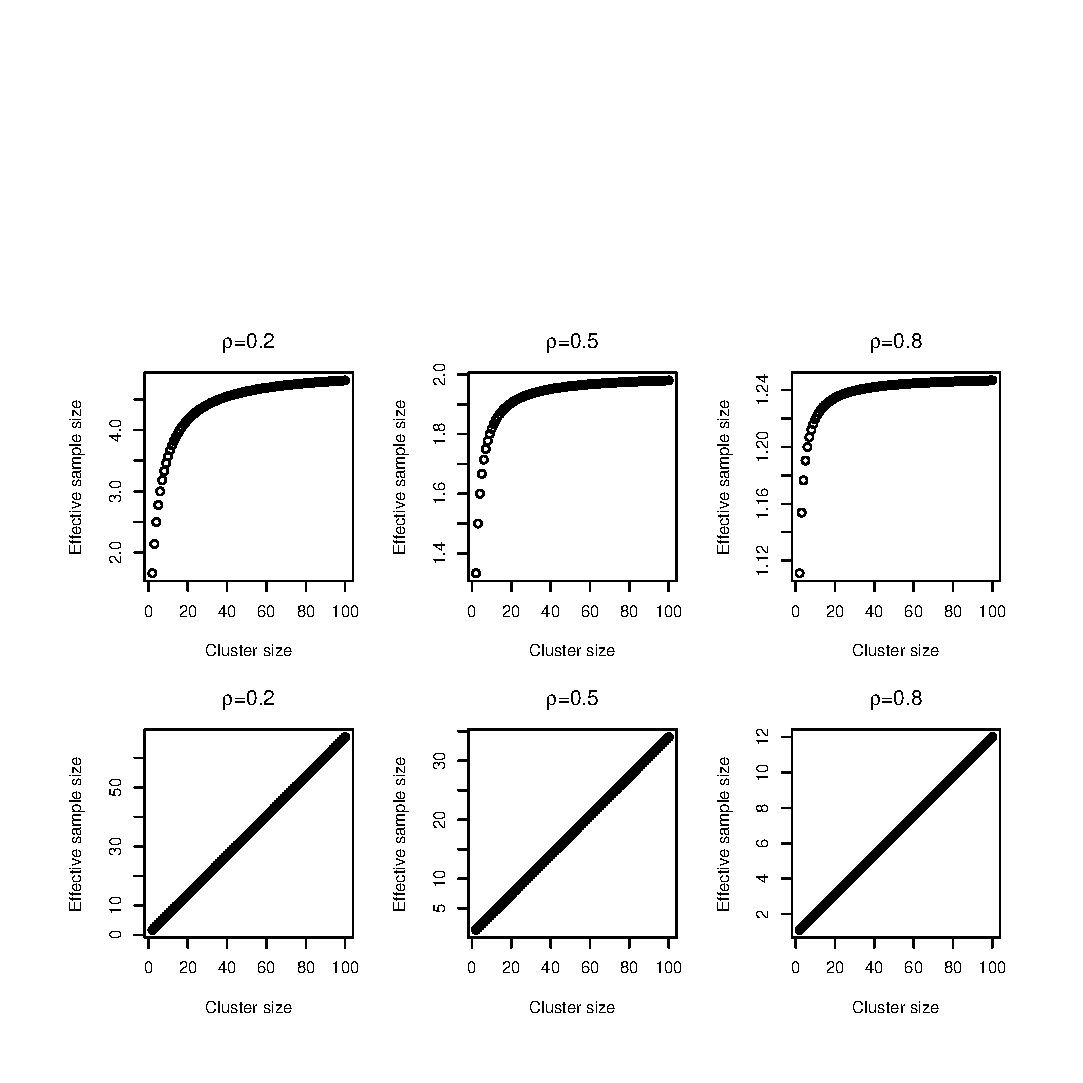
\includegraphics[trim=0mm 9mm 0mm 53mm, clip,width=\textwidth]{fig_ess.eps}
\caption[The effective sample sizes for different cluster sizes for CS and AR(1) covariance structures for different correlation values $\rho$.]{The effective sample sizes (vertical axis) for different cluster sizes for CS (first row) and AR(1) (second row) covariance structures for different correlation values $\rho$.} 
\label{fig_ess}
\end{figure} 


Figure \ref{fig_ess} (first row) shows the effective sample sizes in the CS case for $\rho=\{0.2,0.5,0.8\}$ and $n=\{1,2,\ldots,100\}$. As one may see, the effective sample size in the CS case converges to an asymptote. This value decreases with increasing $\rho$. But no matter the non-zero value of $\rho$, the effective sample size is bounded from above. This follows as the limit of (\ref{effective_cs}):  
\begin{equation}
\label{information_limit}
\lim_{n_i\rightarrow \infty} \frac{n_i}{1+\rho (n_i-1)} = \frac{1}{\rho}.
\end{equation}
This property is called the information limit by \cite{faes2009}.
 Note that this does not apply to negative $\rho$. In that case, the lower limit of the correlation depends on $n$, as it equals $-1/(n-1)$. In other words, should $n\rightarrow\infty$, the correlation cannot be smaller than~$0$, contradicting a negative correlation. Thus, it is sensible to restrict attention to non-negative correlation. This lower bound for the intra-class correlation, $\rho$, comes from the fact that for a smaller $\rho$ the covariance matrix will be non-positive definite, i.e., the variance would be negative.

For positive correlation, the amount of information from  CS clusters is bounded from above. As a consequence, after some point, adding more replications to a cluster would no longer lead to useful efficiency improvements.

To make this point more clearly, consider the variance of estimating the parameter $\mu$ of a multivariate normal vector with CS covariance structure using $N$ clusters all of size $n$. This variance is \cite{Iddi2011}:
\begin{equation}
\label{var_mu_cs}
\mathrm{Var}(\widehat{\mu}_{n})= \frac{\sigma^2 + n \tau}{N n}= \frac{\sigma^2}{Nn} \frac{\left(\sigma^2+ n\tau\right)}{\sigma^2}.
\end{equation}
The quantity $\sigma^2/Nn$ is the variance of $\widehat{\mu}_{n}$ if the data were uncorrelated ($\tau=0$), the factor $\sigma^2 + n\tau / \sigma^2 >1$ is the price we pay because of non-zero correlation in terms of variance. This quantity is often called the variance inflation factor (VIF), i.e., the correlation inflates the variance comparing with the case of non-correlated data. As non-zero correlation would inflate the variance, it deflates the information. We may define the variance deflation factor, VDF, as $1/\mathrm{VIF}$. As one may see, for the CS case, the VIF goes to infinity as $n\rightarrow\infty$. Hence, VDF goes to zero.

The asymptotic relative efficiency (ARE) of estimating $\mu$ with $N$ clusters of size $n\rightarrow \infty$, compared to estimating it using $N$ clusters of finite size $n_f<\infty$ is:
\begin{equation}
\label{eff_cs}
\lim_{n\rightarrow\infty} \frac{\mathrm{Var}(\widehat{\mu}_{n_f})}{\mathrm{Var}(\widehat{\mu}_n)} = \frac{\sigma^2 + \tau n_f}{\tau n_f} = 1+\frac{(1-\rho) }{n_f \rho} >1.
\end{equation}
(This definition, rather than its inverse, is used because ensuing expressions are easiest to manipulate.) Therefore, using a finite random subset of each cluster, the ARE is finite. Hence, one may choose $n_f$ such that the efficiency loss compared to clusters of infinite size becomes arbitrarily small. Indeed, for given $\rho$, set the required ARE equal to $1+\varepsilon$. Then, 
\begin{equation}
\label{nf_var_min_cs}
n_f= \frac{1-\rho}{\rho\varepsilon} = \frac{\sigma^2}{\tau \varepsilon}.
\end{equation}
For example, set $\varepsilon=0.01$, a very small increase of variability. For $\rho=0.5$, $n_f=100$ would reach this goal. Should $\rho=0.9$, then $n_f\simeq 11$ would fulfill the requirement. These are important reductions in big-data settings, or whenever $n_f/n$ becomes very small. The corresponding expression for finite (typically large) $n$ is:
$$n_f=\frac{n(1-\rho)}{\varepsilon(1+\rho+n\rho)+1+\rho}.$$
Considering (\ref{var_mu_cs}), with a cluster of infinite size, the variance is:

\begin{equation}
\label{var_min_cs}
\lim_{n\rightarrow \infty} \frac{\sigma^2 + n \tau}{Nn} = \frac{\tau}{N}.
\end{equation}

In other words, with the given number of clusters, the minimum variance we can reach is (\ref{var_min_cs}). That is to say, in such a situation, for a given number of clusters, increasing the cluster sizes cannot make the variance smaller than a specific value. Obtaining a smaller variance is still possible by adding new clusters (increasing $N$). Such considerations can be found in the literature on determining sample and cluster sizes for cluster randomized trials. For example, \cite{teerenstra2008} have considered a 3-level model, with CS structure for variance at both levels (each with its own correlation); \cite{teerenstra2010} extended these calculations to generalized linear models. The information limit property of CS-based estimators is considered from a different point of view in \cite{feng2001}, \cite{guittet2005}, and \cite{hemming2011}.

\subsection{Finite Information Limit (FIL) Estimators}
\label{sec_FIL}
It is useful to generally define FIL. We also examine some other examples, and provide an important counterexample. 

Consider the same clustered setting as before. Let $\bftheta$ be the parameter of interest and $\widehat{\bftheta}$ a corresponding estimator. Then, $\mathrm{Cov}(\widehat{\bftheta})$ has the FIL property if, for fixed $N$,  $\lim_{n_i \rightarrow \infty} \mathcal{I}_{\bftheta} < \infty$, where $\mathcal{I}_{\bftheta} = \mathrm{Cov}(\widehat{\bftheta}) ^{-1} $ is the Fisher information.

The practical implication is the same as with CS. Let us say that there are $K$ unique cluster sizes among the $n_i$; index these as $n_k$ and assume that for each $k$ there are $c_k$ clusters in the dataset. Then, $N=\sum_{k=1}^K c_k$. Because of FIL, one can consider a cluster size $n_f$, ideally $n_f \ll \min_k\{n_k\}$, such that the efficiency loss is less than a small, pre-specified amount. In some cases, it may be necessary to include all data from the subset of smaller clusters, while sub-sampling the larger clusters. 

In effective sample size terminology, the estimator $\widehat{\bftheta}$ has the FIL property if and only if the difference between effective sample sizes of original and sub-sampled data can be made arbitrarily small. Adopting a VDF viewpoint, $\widehat{\bftheta}$ has the FIL property, if as the cluster size $n\rightarrow\infty$, the VDF goes to zero with at least linear rate.

While CS is a clear example, it is not the only one. Multivariate normal models with variance-covariance structure where the correlation between two replications within a cluster does not approach zero with increasing (spatial or temporal) distance between them are FIL candidates. These include  correlation structures induced by linear mixed models with, for example, random intercept and random slope in time. For practical examples, consider craniofacial growth in rats \cite{verdonck1998}, several products examined by an expert panel \cite{milanzi2014}, genetic data where long sequences of genetic data are available for each subject \cite{sikorska2013}, etc.

Consider a linear mixed model $\BY_i \sim N(X_i\beta, \Sigma_i)$, where $X_i\beta=\mu \mathbf{1}$ and $\Sigma_i=Z_i D Z_i + V_i$. Obviously, the $\mathbf{\bar{Y}}=1/n (\mathbf{1'}\BY_i) \sim N(\mu, 1/n^2 \mathbf{1'} \Sigma_i \mathbf{1})$. The FIL exists if the variance $1/n^2 \mathbf{1'} \Sigma_i \mathbf{1}$ does not go to zero when cluster size tends to infinity. In other words, for a $\sqrt{n}$-consistent estimator, FIL does not apply. 

Evidently, a linear mixed model with only a random intercept and independent errors with variance $\sigma^2$ is identical to the CS model. We have already seen that FIL exists in such a case. For a linear mixed model with random intercept $b_{0i}$ and random slope $b_{1i}$ in time one can derive,

$$\mathrm{Var}(\widehat{\mu_{IS}})= d_{22} \frac{(n+1)^2}{4} + d_{12} (n+1) + d_{11} + \frac{\sigma^2}{n},$$
where $d_{11}=\mathrm{Var}(b_{0i})$, $d_{22}=\mathrm{Var}(b_{1i})$ and $d_{12}=\mathrm{Cov}(b_{0i},b_{1i})$. Also, $IS$ in $\mu_{IS}$ refers to a random intercept-slope model. Obviously, as $n\rightarrow\infty$, $\mathrm{Var}(\widehat{\mu_{IS}}) \rightarrow \infty$, so $\mathcal{I}_{\widehat{\mu_{IS}}}$ is finite and FIL applies in this case as well. If one also looks at the VDF here, it goes to zero at a cubic rate.

Considering the CS case with $\rho=0$, this would be an independent identically distributed sample from $N(\mu,\sigma^2)$. It is well-known and also straightforward to see that the estimator of $\mu$ is $\sqrt{n}-$consistent in this case, hence its variance goes to $0$ as $n$ tends to infinity. Therefore, the information is unbounded. However, such $\sqrt{n}$-consistent estimators are not specific to independent (non-clustered) data. It can happen for correlated (clustered) data as well. 


A clear counterexample of non-FIL for clustered data is the multivariate normal vector with first-order autoregressive (AR(1)) variance-covariance. Then, $\Sigma=\sigma^2 C_n$ where the $(j,k)$ element of $C_n$ is $\rho^{|j-k|}$. Clearly, the correlation between $Y_{ij}$ and $Y_{ik}$ decreases rapidly with $|j-k|$. 

The variance of $\widehat{\mu}$ in this case, based on $N$ clusters of size $n$, is \cite{Lisa2016_3}:
\begin{equation}
\label{var_mu_ar1}
\mathrm{Var}(\widehat{\mu}_{AR1})= \frac{\sigma^2 (1+\rho)}{N [n-(n-2)\rho]}.
\end{equation}
Obviously, 
\begin{equation}
\label{info_ar1}
\lim_{n\rightarrow\infty} \frac{1}{\mathrm{Var}(\widehat{\mu}_{AR1})} = \infty.
\end{equation}
The ARE of $\mathrm{Var}(\widehat{\mu}_{AR1})$ when using $n_f <n$ measurements from each cluster, when $n\rightarrow\infty$, is:
\begin{equation}
\label{eff_ar1}
\lim_{n\rightarrow\infty} \frac{\mathrm{Var}(\widehat{\mu}_{n_f})}{\mathrm{Var}(\widehat{\mu}_n)} = \lim_{n\rightarrow\infty} \frac{(1-\rho) n + 2\rho}{(1-\rho) n _f + 2\rho} = \infty.
\end{equation}
The above follows from the ESS as well. For AR(1), derived \cite{faes2009}:
\begin{equation}
\label{effective_ar1}
\widetilde{n}=\frac{n-(n-2)\rho}{1+\rho}.
\end{equation}
Figure \ref{fig_ess} (second row) shows the effective sample sizes in the AR(1) case for $\rho=\{0.2,0.5,0.8\}$ and $n=\{1,2,\ldots,100\}$. As one may see, from (\ref{effective_ar1}) and the figure, and in contrast to the CS case, no matter what is $\rho$ or $n$, the effective sample size does not converge to any asymptote. Of course, because of the correlation, the ESS is less than $n$; for larger $\rho$'s, the ESS is smaller, but it is not bounded from above. For example, when $\rho=0.5$, $\widetilde{n}=(n+2)/3$; for $\rho=0.9$, we find $\widetilde{n}=(n+18)/19$. Hence, there is no information limit and adding cluster replications will add information without approaching a limit. Related, one may  verify that the VDF for AR(1) case does not goes to zero neither. This property ensures that time-series analysis works for AR(1) structures or one of the many generalizations thereof.

It is worth remarking that, in cases such as AR(1), increasing the cluster size means increasing the distance, $|j-k|$, (spatially, temporally, etc.) between measurements. As is implied by the structure, that would make the correlation smaller, so unlike in cases with FIL property, the correlation here is not persistent. In other words, no matter how large the correlation, if the lag between two measures increases, the correlation between them will become arbitrarily small, so the information added by such a new measurement will become virtually the same as for an independent additional measurement. Therefore, the information is not bounded in such structures.

Although FIL cannot be used to deal with high-dimensional AR(1) data, there are other possible solutions. Recently, \cite{Lisa2016_3} have derived closed-form solutions for AR(1) model parameters in case the cluster sizes are all equal. They presented fast and stable performance of such solutions compared to existing iterative methods. Furthermore, they have proposed a sample-splitting solution to deal with clusters of unequal sizes for the case of AR(1) data. That would extend the use of the derived closed-form solutions in the case of unequally sized clusters.


\subsubsection{Simulations I}
\label{sub_sec_sim1}
A first simulation study is conducted to illustrate the FIL property for CS data. To this end, CS clusters are generated.  Consider $c_k$ clusters of unique sizes $n_k$ for $k=1,\ldots,6$. The simulation settings are:
\begin{itemize}
\item $\mu=0$, $\tau=5$ and $\sigma^2\in\{20,5,1.25\}$ to produce $\rho\in\{0.2,0.5,0.8\}$
\item $n_k\in\{500,600,700,800,900,1000\}$, and $c_k\in\{100,100,100,100,100\}$.
\item $n_f=\{5,10,50\}$. 
\end{itemize}
A set of data is generated 50 times for each setting. Parameters are estimated for the full data using the MIXED procedure in SAS 9.4 for Windows. A sub-sample of size $n_f\in\{5,10,50\}$ is taken and the parameter $\mu$ and its variance  estimated using  balanced-data closed forms \cite{Iddi2011}. The ARE's are computed by comparing the variance using a sub-sample of size $n_f$ with the entire dataset. 

Figure \ref{fig_m1} shows the results for $n_f=\{5,10,50\}$ and $\rho=\{0.2,0.5,0.8\}$. 
Clearly, for $\rho=0.2$, a very high efficiency is reached using the sub-samples of size $n_f=50$, which gets even better for the higher correlations: indeed, when $\rho=0.5$, one can suffice with $n_f=10$, while for $\rho=0.8$, a sub-sample of size $n_f=5$ leads to almost full efficiency.
\begin{figure}[!t]
\centering
\includegraphics[width=\textwidth]{fig_m1.eps}
\caption{Comparing the ARE of full data with sub-samples of sizes $n_f=\{5,10,50\}$ for $\rho=\{0.2,0.5,0.8\}$. The dashed horizontal line shows ARE$=1$.} 
\label{fig_m1}
\end{figure}  
In other words,  even for a correlation as small as $\rho=0.2$, analyzing only $6\%$ of the data produces almost the same efficiency as using the entire dataset. When the correlation becomes as high as $\rho=0.8$, this proportion decreases to as little as $0.6\%$. 

Using such a (tiny) sub-sample has two main advantages. First, the computation time drops substantially. This can be seen from Table~\ref{tab_comp_time}. On the other hand, this  sub-sample can be chosen with all cluster sizes constant, which further enables the use of closed-forms \cite{Lisa2016_1}, further reducing computation time and avoiding any convergence issues. Thus, sacrificing a tiny bit of efficiency can be considered a good bargain. 

\subsection{Extensions}
\label{sec_detect}

From Sections~\ref{sec_CS_effect} and \ref{sec_FIL}, the advantages of FIL are clear. When CS is known to be true or assumed, sub-sampling can be used, unlike in the AR(1) case.  But the question that remains is how to  determine the sub-sampling size, $n_f$.



For the CS case, by pre-specifying the ARE rate, $1+\varepsilon$, one may use (\ref{nf_var_min_cs}) to determine the needed cluster size to achieve the desired level of efficiency comparing with a cluster of infinite size. Of course, the formula in (\ref{nf_var_min_cs}) involves unknown parameters. In practice, one would take a small manageable sub-sample from the data (e.g., $n_f=5$) to estimate the unknown parameters. To consider the extra uncertainty introduced into this estimator via replacing parameters with their estimates, a confidence interval can be constructed for $n_f$ and its upper-bound can be used, to be on the safe side. As (\ref{nf_var_min_cs}) involves the ratio of two random variables (as the parameters are replaced by their estimators), Fieller's method \cite{fieller1954} or the Delta method can be used to find such a confidence interval. Details of calculating such intervals will be provided in~Appendix \ref{app1}. 
%
%As the $n_f$ using (\ref{nf_var_min_cs}) is calculated assuming the CS structure assumption for the variance is valid, one may also compute the variance using $n_f+\ell\; (\ell>0)$. If the CS assumption is true, then it does not imply much more additional efficiency using a sub-sample of size $n_f+\ell$.  

While for a FIL estimator taking only one sub-sample can provide the desired efficiency compared with using the full sample, when computational power available, it worth to consider taking more sub-samples of smaller sizes. Assume a single cluster of size $N$ with multivariate normal distribution and CS structure for its covariance matrix. Suppose we take $M_0$ sub-samples of size $n_0$ from this cluster, we have derived:

\begin{equation}
\label{are2}
\mathrm{ARE}= \frac{1}{2} + \frac{1}{2} \frac{N}{n_0} \frac{1+(n_0-1) \rho}{1+ (N-1) \rho}.
\end{equation}
For example, for sufficiently large $N$, $M_0=2$, $\rho=0.5$, and efficiency equal to $5/4$ one may derive $n_f=2$, i.e., taking only two sub-samples of size 2 would produce such efficient estimators. The ARE's in (\ref{eff_cs}) and (\ref{are2}) are derived in Appendix~\ref{app2}.


As stated earlier, a CS covariance structure is an important example of FIL estimators, while AR(1) is an important counterexample. The next question that needs to be addressed is how to examine, in general terms, whether the model at hand actually allows for a FIL estimator.

A priori, variance-covariance structures purely induced by serial or spatial processes would not be good FIL candidates, while structures induced at least in part by random effects might offer more hope. Still, the above is intutitive only and thus there is the need for a tool to detect this property in cases where the analyst is not sure. Of course, the `ideal' but impractical solution is to analyze the full dataset as well as a small subset of it and to compare the results. While useless as such, it points to an alternative strategy. Because of the very information limit, it is not necessary to compare the use of subsets of size $n_f$ to the full dataset, but rather to a subset of clusters of a larger size, but still smaller than the actual cluster sizes. 

Using the same data setting as before, the following algorithm can be executed:
\begin{enumerate}
\item[Step 1.] Determine $n_{f_\ell}$ for $\ell=1,\ldots,L$ such that $n_{f_1} < n_{f_2}<\ldots< n_{f_L} \ll \min_k\{n_k\}$.
\item[Step 2.] For given $\ell$, take $M$ random sub-samples of size $n_{f_\ell}$ and compute $\widehat{\mu_{\ell m}}$ and its variance $\mathrm{Var}(\widehat{\mu_{\ell m}})$ for $m=1,\ldots,M$. Combine $\mathrm{Var}(\widehat{\mu_{\ell m}})$ ($m=1,\ldots,M$) to obtain $\mathrm{Var}(\widetilde{\mu_{n_{f_\ell}}})$ using the combination rules (\ref{mo_estimate}), (\ref{mo_cov}), and (\ref{mo_s2}). Repeat this step for $\ell=1,\ldots,L$.
\item[Step 3.] If there exists an $\ell$ such that $\frac{\mathrm{Var}(\widetilde{\mu_{n_{f_{\ell}}}})}{\mathrm{Var}(\widetilde{\mu_{n_{f_L}}})} < 1+\varepsilon$, for a pre-specified $\varepsilon$, then the estimator under investigation can be taken to have the FIL property.
\item[Step 4.] In case FIL is concluded in Step 3, the final estimate can be computed using $\overline{\mu}=\sum_{\ell=1}^L w_\ell \widetilde{\mu_\ell}$ and $\mathrm{Var}(\overline{\mu}) = \sum_{\ell=1}^L w_\ell \mathrm{Var}(\widetilde{\mu_\ell})$, where $w_\ell = \frac{n_{f_\ell}}{\sum_{\ell=1}^L n_{f_\ell}}$.
\end{enumerate}
Several remarks are worth making. First, $L=2$ might be enough, but depending on the size of the dataset and the computational power available, one can use more than two $n_f$ to reach better estimators. While usually a very small $L$ is sufficient, this parameter can also be gauged empirically, through similar studies. In other words, this implies that experience will grow through sequences of similar data analyses. Second, the sub-sampling can be done only once for each $n_{f_\ell}$, i.e., $M=1$, whence no combination rules are needed. Third, generating and analyzing the samples for each $(\ell,m)$ pair is an array of independent tasks; doing them in parallel is straightforward. Fourth, the sub-sampling can be done more efficiently by splitting the data based on the cluster sizes; this approach is explained in the Appendix~\ref{app3} and an \textsf{R} implementation of it is presented. Fifth, note that not being FIL does not merely follow from not being able to find an $\ell$ that satisfies the condition in Step 3.

The combination rules in Step 2 are based on the so-called multiple outputation idea \cite{hoffman2001,follmann2003}. Let us briefly sketch the method. Consider $M$ sub-samples of size $n_s$, sampled with replacement. Suppose $\widehat{\bftheta}_m$ as the estimated parameter in the $m$-th sub-sample with $\widehat{\Sigma}_m$ as its covariance. The combined estimate $\widetilde{\bftheta}$ and its variance can be computed using the following combination rule:
\begin{equation}
\label{mo_estimate}
\widetilde{\bftheta}=\frac{1}{M}\sum_{m=1}^M \widehat{\bftheta}_m,
\end{equation}
and its covariance is computed as,
\begin{equation}
\label{mo_cov}
\widetilde{\Sigma} = \frac{1}{M}\sum_{m=1}^M \widehat{\Sigma}_m - \frac{M-1}{M}S^2_{\bftheta},
\end{equation}
where,
\begin{equation}
\label{mo_s2}
S^2_{\bftheta} = \frac{1}{M-1} \sum_{m=1}^M (\widehat{\bftheta}_i-\widetilde{\bftheta}) (\widehat{\bftheta}_m-\widetilde{\bftheta})'.
\end{equation}





\subsubsection{Simulations II}
\label{sub_sec_sim2}
To study the performance of the proposed procedure in Section \ref{sec_detect} the simulation study in Subsection \ref{sub_sec_sim1} is extended by repeating the sub-sampling $M=1,3,5$ times. Again, a set of data is generated 50 times for each $\rho\in\{0.2,0.5,0.8\}$ and then the parameter $\mu$ and its variance are estimated for the full data using the MIXED procedure in SAS 9.4 for Windows. A sub-sample of size $n_f\in \{5,10,50\}$ is taken $M\in\{1,3,5\}$ times. Estimation of  $\mu$ and its variance is done in the same ways as in the first simulation. Two ARE's are computed. First, the variance of each sub-sample (for different combinations of $n_f$ and $M$) is compared with the one from the full data. Second, to study the performance of the detection method in Section~\ref{sec_detect}, the variance of each sub-sample, except the largest one ($n_f=50$, $M=5$) is compared with the variance of the largest sub-sample. Note that the negative ARE in some cases where $M>1$ occurs because of negative variance estimates using the correction in (\ref{mo_cov}). This matter is well-known \cite{follmann2003} and can be avoided by increasing $M$ or simply use $M=1$ with sufficiently large $n_f$.

Figure \ref{fig_02} shows the results for $\rho=0.2$. As one may see in this case using $n_f=5$ is not as efficient as expected. While $n_f=10$ could be accepted, $n_f=50$ ($6.68\%$ of data) provides almost fully efficient results. Looking at Figure~\ref{fig_05} for $\rho=0.5$ establishes that using only $n_f=10$ ($1.33\%$ of data) could provide almost fully efficient results. When it comes to $\rho=0.8$ in Figure~\ref{fig_08}, even using $n_f=5$ ($0.67\%$ of data) is almost fully efficient.

Another interesting observation from Figures~\ref{fig_02}, \ref{fig_05}, and \ref{fig_08} is that the proposed procedure in Section \ref{sec_detect}, i.e., comparing the efficiency with a sufficiently large $n_f$, provides results that are in line with the results when the comparison is done with the full data. This provides evidence that this procedure can be trusted to detect the FIL.
\begin{figure}[!t]
\centering
\includegraphics[width=\textwidth]{fig_02.eps}
\caption[Comparing the ARE of full data and sub-sampling of size $n_f=50$, $M=5$ times with different combinations of $n_f$ and $M$ for $\rho=0.2$.]{Comparing the ARE of full data (the boxplot with background color and solid lines) and sub-sampling of size $n_f=50$, $M=5$ times (the box plots with transparent color and dotted lines) with different combinations of $n_f$ and $M$ for $\rho=0.2$. The dashed horizontal line shows ARE$=1$.} 
\label{fig_02}
\end{figure}  
\begin{figure}[!t]
\centering
\includegraphics[width=\textwidth]{fig_05.eps}
\caption[Comparing the ARE of full data and sub-sampling of size $n_f=50$, $M=5$ times with different combinations of $n_f$ and $M$ for $\rho=0.5$.]{Comparing the ARE of full data (the boxplot with background color and solid lines) and sub-sampling of size $n_f=50$, $M=5$ times (the box plots with transparent color and dotted lines) with different combinations of $n_f$ and $M$ for $\rho=0.5$. The dashed horizontal line shows ARE$=1$.} 
\label{fig_05}
\end{figure}  
\begin{figure}[!t]
\centering
\includegraphics[width=\textwidth]{fig_08.eps}
\caption[Comparing the ARE of full data and sub-sampling of size $n_f=50$, $M=5$ times with different combinations of $n_f$ and $M$ for $\rho=0.8$.]{Comparing the ARE of full data (the boxplot with background color and solid lines) and sub-sampling of size $n_f=50$, $M=5$ times (the box plots with transparent color and dotted lines) with different combinations of $n_f$ and $M$ for $\rho=0.8$. The dashed horizontal line shows ARE$=1$.} 
\label{fig_08}
\end{figure}  
Table \ref{tab_comp_time} shows the computation time using only a tiny sub-sample for different combinations of $n_f$ and $M$, next to the time for analyzing the full data. As one may see, depending on the selected $n_f$ and $M$ the computation could become between 500 to 1700 times faster. We may remark that all the computations are done on a single core in a laptop. Of course, distributing the embarrassingly parallel nature of this methodology among different machines could possibly boost the computation more than this. 
\begin{table}[ht]
\caption[Computation time (in seconds) for different combinations of $n_f$ and $M$ and the full data.]{Computation time (in seconds) for different combinations of $n_f$ and $M$ and the full data. The results from different $\rho$'s are aggregated for each combination of $n_f$ and $M$.}
\label{tab_comp_time}
\centering
\begin{tabular}{ccrr}
  \hline \hline
\multirow{2}{*}{$M$} & \multirow{2}{*}{$n_f$} & \multicolumn{2}{c}{Computation time} \\ 
 &  & \multicolumn{1}{c}{Mean} & \multicolumn{1}{c}{SD} \\ 
  \hline
\multirow{3}{*}{$1$} &  5 & 0.704 & 0.059 \\ 
 & 10 & 0.671 & 0.034 \\ 
 & 50 & 0.710 & 0.043 \\ 
\multirow{3}{*}{$3$} & 5 & 1.171 & 0.058 \\ 
 & 10 & 1.158 & 0.056 \\ 
 & 50 & 1.311 & 0.066 \\ 
\multirow{3}{*}{$5$} & 5 & 1.613 & 0.075 \\ 
 & 10 & 1.638 & 0.089 \\ 
 & 50 & 1.981 & 0.094 \\ 
\multicolumn{2}{c}{Full sample} & 1133.973 & 153.387 \\ 
   \hline \hline
\end{tabular}
\end{table}
Finally, as the FIL is detected using $\rho=0.2,05,0.8$, following Step 4 in the FIL detection procedure, one can improve the estimation by combining the results from $M=1,3,5$ using weights proportional to the corresponding $n_f$. Figure~\ref{fig_comb} shows the results of ARE's after taking the weighted average. A further ARE improvement is observed, compared with Figure~\ref{fig_m1}, where for $\rho=0.2$ the upper bound of the ARE is around 2, while after combining the multiple sub-samples, it decreases to around 1.2; the corresponding decrease for $\rho=0.5$ is from 1.25 to 1.06, and still for $\rho=0.9$, from 1.10 to 1.02. 
\begin{figure}[!t]
\centering
\includegraphics[width=\textwidth]{fig_comb.eps}
\caption{Comparing the ARE of full data with sub-samples of sizes $n_f=5,10,50$ when the results from $M=1,3,5$ are combined using the weights $w_i= (5/65,10/65,50/65)$.} 
\label{fig_comb}
\end{figure}  


\subsection{Case study: Amazon.com book ratings}
\label{sec_case_study}
The effectiveness of detecting FIL is examined via simulations in Sections~\ref{sub_sec_sim1} and \ref{sub_sec_sim2}. In this section, we consider the ratings of the books on the Amazon website. The data are obtained from \cite{amazon}. The dataset contains $2,330,066$ books, which are rated at least $1$ and at most $21,398$ times. Obviously, this is an example of clustered data, as the same book is rated many times. Figure \ref{fig_hist} shows the histogram of the number of all and unique cluster sizes.


\begin{figure}[!t]
\centering
\includegraphics[width=\textwidth,trim=0 85 0 0]{fig_hist_full_clust_size.eps}
\caption[Histogram of number of all and unique cluster sizes in Amazon books ratings data.]{Histogram of number of all (left) and unique (right) cluster sizes in Amazon books ratings data.} 
\label{fig_hist}
\end{figure}  


Fitting the CS model to the full data is not feasible; attempting it in Proc MIXED in SAS would lead to the same error as in the Table~\ref{tab_sas}. Therefore, detecting FIL and applying it would make it possible to fit a model to this data. As a CS model is used, following the discussions in Section~\ref{sec_detect}, one may use Fieller's upper-bound of (\ref{nf_var_min_cs}) to determine the sub-sampling size for a pre-specified $\varepsilon$. To estimate the parameters, a sub-sample of size $n_1=5$ is used. Figure \ref{fig_nf} shows the esimated Fieller's upper-bound for $n_f$ for several $\varepsilon$'s using $\alpha=0.05$. As one may see, $\varepsilon \approx 0.09$ can be obtained by a sub-sample of size almost $50$. In order to make sure whether $n_f=50$ is good enough, a sub-sample of size $n_f=100$ is also taken for the sake of comparison.




\begin{figure}[!t]
\centering
\includegraphics[width=\textwidth]{fig_nf_epsilon_full.eps}
\caption{Amazon books ratings data. Fieller's upper-bound of $n_f$ (log-scale) for different values of $\varepsilon$ using $\alpha=0.05$. The parameters are estimated using a sub-sample of size $n_1=5$.} 
\label{fig_nf}
\end{figure}  

The results of model fitting using $n_f=5,50,$ and $100$ are given in Table~\ref{tab_amazon_est}. As one may see for estimating $\mu$, the efficiency using $n_f=50$ comparing with $n_f=100$ does not change substantially (efficiency is equal to $0.99699$). Therefore, one may conclude the FIL property applies and using a sub-set of size $n_f=50$ or $100$ one may be almost as efficient as using the full data. So, while fitting the model to the full data is not feasible, we could obtain almost fully efficient estimates using only a sub-set of the data.

As one may see in Table~\ref{tab_amazon_est}, $\widehat{\rho}=0.17$ and is significant. Another interesting point about these results is that the average rating is estimated as $4.3$. Taking this into account that the maximum possible rating is $5$, this shows those people who like a book tend to rate it. That would lead to an important conclusion: no matter how large the data set is, an inappropriate model may lead to biased estimates, i.e., the majority of the respondents are among the people who have liked the book, so it would not be a representative sample. This matter needs to be foreseen in the model.
\begin{table}[ht]
\centering
\caption{Estimating parameter vector $(\mu,\tau,\sigma^2)$ and its standard error using $n_f=5,50,100$.}
\label{tab_amazon_est}
\begin{tabular}{ccccccc}
  \hline\hline
 $n_f$& \multicolumn{2}{c}{$\mu$} & \multicolumn{2}{c}{$\tau$} & \multicolumn{2}{c}{$\sigma^2$}\\
 & Estimate & StdErr & Estimate & StdErr & Estimate & StdErr \\ 
  \hline
5 & 4.30390 & 0.00053 & 0.22737 & 0.00061 & 1.03355 & 0.00069 \\ 
  50 & 4.30505 & 0.00048 & 0.21496 & 0.00046 & 1.03127 & 0.00040 \\ 
  100 & 4.30500 & 0.00048 & 0.21435 & 0.00046 & 1.03285 & 0.00037 \\ 
   \hline\hline
\end{tabular}
\end{table}

It is worth noting that, as in any model, some assumptions are made here. The two main assumptions considered in this section are normality of the ratings and the CS structure for their covariance matrix. We admit that extensions would be needed for other classes of models, but normality if not crucial for the current setting, as inferences are robust with respect to deviations from normality, especially in the linear model. The CS structure assumption states that two observations can be exchanged, i.e., that observers have similar characteristics. If not, extensions with covariates might be of interest (to correct for such differences), or one may consider separate analyses for different groups of observers. 




\subsection{Conclusion}
\label{cssec_conclusions}
Inspired by compound-symmetry models for clustered data, the finite information limit (FIL) property for estimators based on hierarchical data  is proposed and investigated both theoretically and via simulations. Loosely speaking, FIL means that for increasing cluster sizes, the amount of information is bounded from above. This implies that, after some point, adding new measurements would not substantially add to the information provided by the data, hence the efficiency would not importantly increase further. A consequence of this property is that analyzing a small, or sometimes even tiny, fraction of a dataset with FIL property (e.g., 1\%--2\%) would produce results  almost as efficient as using the entire dataset, see Figures \ref{fig_m1}--\ref{fig_comb}. This property is investigated from a theoretical point of view and a simple procedure is proposed to detect the property in a dataset. This is not needed if simple models known to have the FIL property, such as CS, are used. However, with complex variance-covariance structures, such an empirical check can be handy. 
The proposed procedure together with the FIL itself were investigated in simulation studies. Furthermore, an efficient sub-sampling procedure is implemented in \textsf{R} and available in the Appendix.

Investigating the FIL property on the Amazon.com book ratings enabled us to fit a model which was not feasible for the full data. Based on the obtained results, the efficiency loss was not substantial neither. Such examples would show the importance of properties like FIL to deal with large clustered data, specially when an analysis is needed on a daily basis.

The computation time gain can be enormous, see Table \ref{tab_comp_time}. To add to the computational  efficiency, unlike in many raw dataset, the sub-sample may be chosen balanced,  which adds to the computational efficiency \cite{Lisa2016_1}). As proposed in Section~\ref{sec_detect}, the sub-sampling can be repeated several times to increase efficiency. In addition to the  advantages mentioned, the proposed procedure based on the sub-sampling of various sizes several times consists of so-called ``embarrassingly parallel steps." Therefore, it can be implemented as fast as the computational resources allow. Even on a single core laptop scale, the computation gain could become 1500 times faster than using the full data. One may note that fitting the model to the full (unbalanced) data is usually and out of necessity done using iterative algorithms, which are very complex to make parallel.


\chapter{Structured Vertical Splitting}
\label{chap_structured_vertical}
In this chapter we review the structured vertical splitting with its application in pairwise modeling of several responses simultaneously. 

\section[Fast precision estimation]{Fast precision estimation in high‐dimensional multivariate joint models}


\subsection{Introduction}
\label{sec_intro}

There are different approaches to deal with modelling multivariate clustered data. Authors like \cite{pawitan1993} proposed to analyze each response conditioned on all the others. As an alternative, one may specify a marginal model for each response separately and then join them using an appropriate way. Among such ways are using a latent variable \citep{catalano1992}, copulas \citep{nelsen2007}, or random effects \citep{laird1982}. The latter is of interest in this short note. 

%In the joint modelling approach of multivariate repeated measurements data using random effects, a mixed model is considered for each response separately. Then, the random effects of these models are considered to follow a multivariate distribution which would reflect the association between different responses.

Let $y_{rij}$ be the $j$th measurement taken on the $i$th cluster for the $r$th outcome, $i=1,\ldots,N$, $r=1,\ldots,m$ and $j=1,\ldots,n_{ri}$. Obviously, the number of measurements available for subject $i$ is $\sum_{r=1}^m n_{ri}$. Note that the various outcomes do not need to be of the same kind (continuous, binary, count data, etc.). Also there is no need to have sequences of the same length for each cluster or each outcome. Let $\mathbf{Y_{ri}}$ be the $n_{ri}$ measurements taken on cluster $i$ for outcome $r$. The model assumes that each $\mathbf{Y_{ij}}$ satisfies a mixed model:
\begin{equation}
\label{mixed_model}
\mathbf{Y_{ri}} = \boldsymbol{\mu_{ri}} + \epsilon_{ri},
\end{equation}
where
\begin{equation}
\label{mu_function}
\mathbf{\mu_{ri}} = \mathbf{h}(X_{ri} \boldsymbol{\beta_r} + Z_{ri} \mathbf{b_{ri}}).
\end{equation}
As one may see in (\ref{mu_function}), each outcome can have its own set of fixed effects. In order to capture the associations between different responses, the mixed model approach for joint modelling of the $m$ outcomes allows for correlation between the random effects of each outcome. Let $\mathbf{b_i} = (\mathbf{b_{1i}},\ldots,\mathbf{b_{mi}})'$; the joint model assumes:
\begin{equation}
\label{random_effect_dist}
\mathbf{b_i}=
\begin{bmatrix}
b_{1i} \\
b_{2i}\\
\vdots\\
b_{mi}\\
\end{bmatrix} \sim N \left ( 
\begin{bmatrix}
0 \\
0\\
\vdots\\
0\\
\end{bmatrix}, 
D=\begin{bmatrix}
D_{11} & D_{12} & \ldots & D_{1m}\\
D_{21} & D_{22} & \ldots & D_{2r}\\
\vdots & \vdots & \ddots & \vdots\\
D_{m1} & D_{r2} & \ldots & D_{mm}\\
\end{bmatrix}
\right).
\end{equation}
The matrix $D_{rs}$ ($r,s=1,\ldots,m$) represents the covariance between $\mathbf{b_{ri}}$ and $\mathbf{b_{si}}$. 

While using the joint modelling approach for the multivariate clustered data is a flexible methodology, it can easily become intractable when the number of outcomes becomes large. As the matrix D contains the association between all outcome sequences, its dimension can quickly grow large. Therefore, it is easily possible that such a flexible joint model cannot be used in practice. 

In order to overcome this drawback, \cite{Verbeke2006} and \cite{Verbeke2007} proposed a pseudo-likelihood based approach which considers all possible pairs (or higher order subsets) of the $r$ outcomes and fit them separately. Obviously, using this methodology some parameters are estimated more than once. Averaging multiply estimated parameters gives a final estimate for each parameter. To find a correct estimate of the variance, \cite{Verbeke2006} and \cite{Verbeke2007} proposed a sandwich-type correction of the form $J^{-1}KJ^{-1}$, where $J$ and $K$ are formed based on cluster-wise Hessians and gradients of the log-pseudo-likelihood function, respectively. 

The need for cluster-wise derivatives of the first and second order makes computing this sandwich estimator difficult and possibly expensive. \cite{pair_lin} and \cite{kundu} provided {\tt{SAS}} implementations for the case of linear mixed models. Also, \cite{pair_gen} considered the case of generalized linear models using {\tt{Proc NLMIXED}} in {\tt{SAS}}. However, the cluster-wise calculation can become very expensive for large samples. Also, the focus of these implementations is on the fixed effects only. Implementing the variance estimation for, e.g., matrix $D$ (\ref{random_effect_dist}) is far more complicated. Also, obtaining the right precision quantities in commonly available software like {\tt{R}} demands new implementations. Furthermore, a different model needs its own implementation which includes evaluating gradients and Hessians of the log-(pseudo-)likelihood function. 

\cite{hoffman2001} proposed within-cluster re-sampling to analyze clustered data when the intra-class correlation is considered a nuisance. Their idea was explored in \cite{follmann2003} who gave it the name multiple outputation (MO). MO consists of repeatedly taking sub-samples of size $1$ from each cluster to form a sub-sample of independent observations, to then apply the standard methodologies for such data. The estimated parameters  and their precisions from several sub-samples will be combined using appropriate rules. \cite{hoffman2001} have shown that their variance estimator is consistent.



{\color{black}{Note that using pairs of variables instead of analyzing them jointly is a trick which is not restricted to likelihood-based methods. It has been used in different contexts. For example, \cite{aas2009} have used pair-copulas to model complex multivariate dependencies. Especially with Gaussian outcomes, pairwise approaches (e.g., vine copulas) allow retrieval of the full multivariate association structure, without the need for full joint modelling.}}



In this short note we extend the idea of MO to compute the variance of a pairwise-fitted multivariate joint model as a faster and easier way. The MO-based correction for the variance will be presented in Section~\ref{sec_method}. A simulation study will compare its performance with a sandwich correction in Section~\ref{sec_sim}. The two corrections are compared in analyzing a real dataset in Section~\ref{sec_application}, and finally the paper is concluded in Section~\ref{sec_conclusions}.

\subsection{A fast variance estimator based on multiple outputation}
\label{sec_method}
Consider $y^{(s)}_{rij}$ as the $j$th measurement on $i$th cluster for $r$th outcome in the $s$th sub-sample, where $s=1,\ldots ,M$, $j=1,\ldots,n_{ri}$, $i\in \{1,\ldots,N\}$, and $r\in \{1,\ldots,m\}$. Also consider $\boldsymbol{\theta}^{(s)}$ a vector of size $p_s$ ($s=1,\ldots,M$), containing parameters estimated using the variables involved in the $s$th sub-sample, obviously, $\boldsymbol{\theta}^{(s)} \subseteq \boldsymbol{\theta}$. Let $\boldsymbol{\Theta}' = (\boldsymbol{\theta}^{(1)},\ldots,\boldsymbol{\theta}^{(M)})$ the stacked vector combining all parameters estimated in different sub-samples. $\widehat{\boldsymbol{\Theta}}$ replaces each $\boldsymbol{\theta}^{(s)}$ by its estimate. Also, $\boldsymbol{\Sigma}_{\boldsymbol{\Theta}}$ is a vector of length $\sum_{s=1}^M\times p_s$, with its elements the variance of each element of $\widehat{\boldsymbol{\Theta}}$.


The MO in the current paper extends the one in \cite{hoffman2001} and \cite{follmann2003} in two main directions. First, the sub-samples in our approach are of size larger than one. The second aspect of our proposed extension of MO concerns the sub-sampling scheme. The MO in the sense of \cite{hoffman2001} and \cite{follmann2003} takes random sub-samples of size $1$ from each cluster many times to form sub-samples of independent observations. In our approach, the sub-samples are not taken at random but based on a pre-defined structure which implies a fixed number of needed sub-samples.  {\color{black}{{One may note that the sub-sampling in our proposal is performed at the response level. Therefore, as it is not necessary to measure every response for all subjects, each subject will be presented in the sub-samples which the responses presented there are measured for it.}}} 

For example, using a pairwise approach, each sub-sample consists of all the observations available for each subject corresponding to the two outcomes in the pair under analysis. Therefore, having $m$ outcomes, we need to take $M=m(m-1)/2$ sub-samples, each with a size larger than one. Note that, in a pairwise approach, $M=m(m-1)/2$ is the number of all possible sub-samples. Taking less sub-samples would fail to estimate some parameters. On other hand, taking more sub-samples is not possible without repeating some already taken sub-samples.  {\color{black}{{As it was remarked, it is not necessary for every subject to be present in every sub-sample. In a pairwise approach, suppose we only have three responses $y_1,y_2,y_3$ and for a particular subject only $y_1$ is measured. Then this subject will only be present in pairs $(y_1,y_2)$ and $(y_1,y_3)$.}}}


%Note that in a pairwise modelling approach, each sub-sample consists of the measurements corresponding to one pair of outcomes. Therefore, having $m$ outcomes, we have $M=m(m-1)/2$ sub-samples. For example, the sub-sample corresponding to the first pair (first and second responses) would consists of $\sum_{j=1}^K (n_{1j}+n_{2j})$ observations. This can be considered an extension of MO in the sense of \cite{hoffman2001} and \cite{follmann2003} that takes sub-samples of size one from each cluster.



As one may have already noticed, some of the parameters in $\boldsymbol{\theta}$ would have more than one counterpart in $\boldsymbol{\Theta}$. In order to bring the $\boldsymbol{\Theta}$ back to the desired parameter space, one may take the average of possible several counterparts of each element of $\boldsymbol{\theta}$ in $\boldsymbol{\Theta}$. This can be done using an appropriate weight matrix pre-multiplied by $\boldsymbol{\Theta}$. Consider $A$, a $(p\times \sum_{s=1}^M p_s)$ matrix where its $(\ell,k)$th element, $\ell=1,\ldots,p$, $k=1,\ldots, (p\times \sum_{s=1}^M p_s)$, is defined as follows:


\begin{equation}
\label{matrix_A}
A_{\ell,k} = \left\{
\begin{array}{rl}
1 & \text{if } \boldsymbol{\Theta}_{k} \text{ is a {\color{black}{component}} of } \boldsymbol{\theta}_{\ell},\\
0 & \text{otherwise},
\end{array} \right.
\end{equation}


where $\boldsymbol{\Theta}_{k}$ and $\boldsymbol{\theta}_{\ell}$ are the $k$th and $\ell$th elements in $\boldsymbol{\Theta}$ and $\boldsymbol{\theta}$, respectively. If $W$ is defined as $A$ but with the rows divided by their sum then the combination rules for combining the estimates from $M$ sub-samples are as follows,
%\begin{equation}
%\label{comb_rules}
%\begin{cases}
%\widetilde{\boldsymbol{\theta}} = W \widehat{\boldsymbol{\Theta}},\\
%\mathrm{diag}\left\{\mathrm{Var}(\widetilde{\boldsymbol{\theta}} )\right\}=  W \boldsymbol{\Sigma}_{\boldsymbol{\Theta}} - \mathrm{diag}\left\{W \left(\widehat{\boldsymbol{\Theta}}-\bar{\boldsymbol{\Theta}} \right) \left(\widehat{\boldsymbol{\Theta}}-\bar{\boldsymbol{\Theta}} \right)' W'\right\},
%\end{cases}
%\end{equation}



\begin{equation}
\label{appendix_comb_rules}
\begin{cases}
\widetilde{\boldsymbol{\theta}} = W \widehat{\boldsymbol{\Theta}},\\
{\color{black}{\mathrm{diag}\left\{\mathrm{Var}(\widetilde{\boldsymbol{\theta}} )\right\}=  W \boldsymbol{\Sigma}_{\boldsymbol{\Theta}} - W \mathrm{diag}\left\{\left(\widehat{\boldsymbol{\Theta}}-\bar{\boldsymbol{\Theta}} \right) \left(\widehat{\boldsymbol{\Theta}}-\bar{\boldsymbol{\Theta}} \right)' \right\}}},
\end{cases}
\end{equation}

where $A'$ is the transpose of $A$, and $\bar{\boldsymbol{\Theta}} = \widehat{\boldsymbol{\Theta}} - A' \tilde{\boldsymbol{\theta}}$. For the proof, see \citet[][Appendix 2]{hoffman2001}. These authors have shown that $I^{1/2} ( \widetilde{\boldsymbol{\theta}} - \boldsymbol{\theta}) \xrightarrow{d} N(0, \Sigma)$, where $\xrightarrow{d}$ means convergence in distribution and $\mathrm{Var}(\widetilde{\boldsymbol{\theta}} )$ is a consistent estimator of $\Sigma$.

We may note that the combination rules in (\ref{appendix_comb_rules}) are only estimating the diagonal elements of the covariance matrix of $\widetilde{\boldsymbol{\theta}}$.  If one is interested in estimating the off-diagonal elements as well, the combination rules are the same. One would only need to construct $\boldsymbol{\Sigma}_{\boldsymbol{\Theta}}$, which takes into account the off-diagonal elements also, then an appropriate $W$ can be used to combine the estimated variances and covariances obtained from each sub-sample. The corresponding vector of unique parameters in this covariance matrix would be $p(p+1)/2$, where each sub-sample would estimate part of them. 


{\color{black}{As one may see in (\ref{appendix_comb_rules}), the combination rule for the variance has a subtraction, so as pointed out by both \cite{hoffman2001} and \cite{follmann2003}, theoretically, it is possible to estimate a non-positive definite covariance matrix. Although the chance for such an occurrence is small, and we have not observed it even once in our simulations, it is still necessary to discuss this matter. We can consider three situations in which such a phenomenon would occur: (1) the sample size, $N$, is not sufficiently large, (2) the number of sub-samples, $M$, is not sufficiently large, and (3) the size of each sub-sample is not sufficiently large.

\cite{hoffman2001} proposed to increase the number of sub-samples, $M$, to solve this problem. As it was pointed out, unlike the usual MO, in our approach the number of sub-samples is fixed. Therefore, in case of a non-positive definite covariance estimate, we suggest to take larger sub-samples each time. Note that taking such a strategy is not possible in the usual MO, since it takes one observation per cluster, so the sub-sampling size is fixed. Taking larger sub-samples in our case means to consider triples, quadruples, etc., instead of pairs. We expect the problem of non-positive definite covariance estimate to vanish when taking larger sub-samples. 

When maximum likelihood estimator (MLE) is used, \cite{follmann2003} proposed a variance estimator based on MLE approximation, using first order Taylor expansion of the score function. This approach requires the evaluation of the subject-wise gradient and Hessian of the log-likelihood function, which is similar to the requirements of the sandwich estimator. Therefore, in case where even with larger sub-samples a non-positive definite covariance estimate persists, we suggest to use the sandwich estimator instead of MO.}} 





\subsection{Simulations}
\label{sec_sim}
In this section the proposed idea will be explored and examined via two simulations studies. Sub-section~\ref{subsec_lin} considers joint modelling of linear mixed models, and Sub-section~\ref{subsec_genlin} takes a joint model of ordinal data in a generalized linear mixed models context.

\subsubsection{Gaussian responses}
\label{subsec_lin}
Consider the linear case with identity link in (\ref{mu_function}), as follows:
\begin{equation}
\label{lin_mixed}
\BY_i= X_i \beta + Z_i \Bb_i + \epsilon_i,
\end{equation}
where $X_i$ is the design matrix regarding fixed effects, $\beta$ represents the fixed effects, $Z_i$ is the design matrix related to the random effects, and $\Bb\sim N(0,D)$ shows the random effects. The errors are represented by $\epsilon_i\sim N(0,R)$. In order to evaluate the proposed method in a simulation study, consider the model in (\ref{lin_mixed}) with parameters:

\begin{equation}
\label{sim_params}
\beta=(5,5,5,5), D= \left(
\begin{array}{cccc}
60 & 40 & 25 & 40 \\
& 50 & 35& 30 \\
& & 45 & 40 \\
&&&55
\end{array} \right), R= 196 I_{n_i},
\end{equation}
where $I_{n_i}$ is the identity matrix of order $n_i$, with $n_i$ the length of the $i$-th cluster. {\color{black}{This means that both of the $X_i$ and $Z_i$ are formed by columns of $1$'s.}} The data are generated from such model 100 times, each consists of 100 clusters of size $n_i=5$. The mixed model is fitted to the full sample as well as each of the 6 pairs using Proc MIXED in {\tt{SAS}}. Then, the estimates and variances are combined using (\ref{appendix_comb_rules}). Also, the sandwich estimator is calculated using {\tt{\%jointpair}} macro in {\tt{SAS}} in \cite{pair_lin}.

Figure \ref{fig_sim} shows the simulation results. As one may see, the relative efficiency of estimating fixed effects using sandwich and MO corrections are very similar. Furthermore, the relative efficiency for estimating parameters in the $D$ matrix are also presented. These parameters are only estimated using the MO correction, as the implementation was not available for sandwich-correction. The interesting result here is the computation time. As one may see, using MO-correction the computation can be done more than 2500 times faster. On the other hand, in case that computing the full likelihood model is possible (as it is the case in our simulation study), MO-correction can also possibly be computed faster than the full-likelihood. Therefore, it is not only an alternative for infeasible likelihoods, but also, it can be used to accelerate computations that are strictly speaking doable.

%\begin{figure}
%\centering
%\includegraphics[width=\textwidth,trim=0 110 0 120]{fig_sim.eps}
%\caption{Histogram of computation time using IMO and sandwich corrections.} 
%\label{fig_scatter2}
%\end{figure} 


\begin{figure}[htb]
\begin{center}
\includegraphics[width=\textwidth]{fig_sim_eq_new.eps}
\caption[Simulations (Gaussian outcomes) comparing sandwich and MO corrections separately]{Simulations {\color{black}{(Gaussian outcomes)}}. Top: Relative efficiency of estimated fixed effects using MO-correction (left) and sandwich-correction (middle), estimated $D$-matrix using MO-correction (right) compared to the full model. {\color{black}{The relative efficiency is defined as the ratio of the variance of the alternative method and the full likelihood, e.g., for MO $\mathrm{Var}(\widetilde{\theta}_{\mathrm{MO}})/\mathrm{Var}(\widehat{\theta}_{\mathrm{full}})$ is computed}}. Bottom: Histograms of computation time (in seconds) using sandwich and MO corrections (first and second). Histograms of computation time (in seconds) using sandwich and MO corrections (third and fourth) relative to the full model computation time.}
\label{fig_sim}
\end{center}
\end{figure}



{\color{black}{
In order to see how our proposal performs comparing with sandwich estimator when the correlation between the random effects is small, the simulation above is repeated, but this time the off-diagonal elements of $D$ matrix in (\ref{sim_params}) are divided by $10$. Figure~\ref{fig_sim_small} shows the relative efficiencies of the variances obtained using MO and sandwich corrections. As one may see, these relative efficiencies are again very close to $1$.

\begin{figure}[htb]
\begin{center}
\includegraphics[width=\textwidth]{fig_sim_small.eps}
\caption[Simulations (Gaussian outcomes): comparing sandwich and MO corrections]{{{Simulations (Gaussian outcomes). Top: Relative efficiency of estimated fixed effects using MO-correction (left) and sandwich-correction (right). Bottom: estimated $D$-matrix using MO-correction compared to the full model. The relative efficiency is defined as the ratio of the variance of the alternative method and the full likelihood, e.g., for MO $\mathrm{Var}(\widetilde{\theta}_{\mathrm{MO}})/\mathrm{Var}(\widehat{\theta}_{\mathrm{full}})$ is computed.}}}
\label{fig_sim_small}
\end{center}
\end{figure}
}}



{\color{black}{

\subsubsection{Non-Gaussian responses}
\label{subsec_genlin}

In order to investigate the performance of our proposal for non-Gaussian responses and more complex models a simulation is done based on the Leuven diabetes project. This dataset is analyzed in \cite{ivanova2015}, details about this study can be found there. Here we only review parts necessary for our simulations. In order to study how well the diabetes is controlled, three outcomes were measured for each patient at baseline ($T_0$) and one year later ($T_1$). These three outcomes of interest were LDL-cholesterol (low-density lipoprotein cholesterol, mg/dl), HbA1c (glycosylated hemoglobin, \%), and SBP (systolic blood pressure, mmHg). Although these three variables are continuous, the interest was in expert-specified cut-off values of these outcomes. The cut-off values are defined as $\{<100, [100,115), [115, 130),\geq 130 \}$ (mg/dl) for LDL-cholesterol, $\{<7, [7, 8), \geq 8\}\%$ for HbA1c, and $\{ \leq 130, (30,140],(140,160],>160\}$mmHg for SBP.

In order to analyze these 3 ordinal outcomes together, a joint modelling approach with a proportional odds mixed model (POMM) for each response was considered in \cite{ivanova2015}. The POMM for each response is as follows:
\begin{equation}
\label{sim2_model}
\mathrm{logit}[P(Y_{rij}<k)] = \xi_{r0k} + \xi_{r1} t_{ij} + \xi_{r2} X_{i} + b_{ri} + \epsilon_{rij},
\end{equation}
where $r=1,2,3$ indicates the outcome of interest, and $k=1,\ldots,K-1$ with $K$ as the number of levels of the corresponding outcome of interest. Furthermore, $X_i$ shows the gender of the subject, and $b_{ri}$'s are the random intercepts corresponding to each outcome. Following the mixed model approach for joint modelling of multiple outcomes, we assume the three random intercepts to be normally distributed with the following covariance matrix.

\begin{equation}
\label{sim2_random_effect_dist}
\begin{bmatrix}
b_{1i} \\
b_{2i}\\
b_{3i}\\
\end{bmatrix} \sim N \left ( 
\begin{bmatrix}
0 \\
0\\
0\\
\end{bmatrix}, 
D=\begin{bmatrix}
D_{11} & D_{12} & D_{13}\\
 & D_{22} & D_{23}\\
&& D_{33}\\
\end{bmatrix}
\right).
\end{equation}
The parameter values for generating the data were obtained by fitting the joint model to the Leuven diabetes dataset. The data were generated $200$ times using {\tt{SAS Proc IML}}. Each time the parameters in the $3$ pairs were estimated using adaptive Gaussian quadrature \citep{pinheiro1995} with $3$ quadrature points in {\tt{SAS Proc NLMIXED}} and the combined variance was estimated using sandwich and MO corrections. Considering the complexity of the model, in order to do the simulation quicker, the codes were run on VSC cluster in Leuven, Belgium.

The results of the simulations are summarized in Table~\ref{tab_sim2}. Column 3 of Table~\ref{tab_sim2} shows the parameter values which were used to generate the data. The last three columns show the means and standard deviations over 200 replications for estimated variance using MO, sandwich, and their relative efficiency, respectively. As one may see, for all of the variables the estimated variances are very close, therefore, one can conclude that our proposal performs well also in a complex model with non-Gaussian responses.

\begin{table}[ht]
\centering
{{
\caption[Simulations (non-Gaussian outcomes)]{Simulations (non-Gaussian outcomes). The estimated model for three ordinal outcomes. The first columns indicates different outcomes, and the second columnn shows the estimated effect. The data obtained parameter-values which were used to generate the data are presented in column 3. Columns four and five show the average (standard deviation) of standard error using MO and sandwich, obtained over 200 replications, respectively. The last column shows the relative efficiency of MO compared to sandwich: $\mathrm{Var}(\widetilde{\theta}_{\mathrm{MO}})/\mathrm{Var}(\widetilde{\theta}_{\mathrm{Sandwich}})$.}
\label{tab_sim2}
\resizebox{\textwidth}{!}{\begin{tabular}{lllccc}
  \hline
Outcome&Effect&Parameter & MO & Sandiwch & ARE (MO/Sandwich)  \\ 
  \hline \vspace*{1mm} 
\multirow{4}{*}{LDL-chol.}&Int. 1&$\xi_{101}=-0.740$ & 0.039 (0.006) & 0.039 (0.006) & 0.993 (0.009)  \\ \vspace*{1mm} 
&Int. 2&  $\xi_{102}=0.480$ & 0.038 (0.006) & 0.038 (0.006) & 0.998 (0.009)  \\ \vspace*{1mm} 
&Int. 3 & $\xi_{103}=1.580$ & 0.042 (0.006) & 0.041 (0.007) & 1.012 (0.010)  \\ \vspace*{1mm} 
&Time  &$\xi_{11}=1.050$ & 0.032 (0.004) & 0.032 (0.004) & 1.024 (0.008)  \\ \vspace*{1mm} 
&Gender  &$\xi_{12}=0.450$ & 0.048 (0.008) & 0.048 (0.008) & 0.989 (0.001) \\ \vspace*{1mm} 
&RI sd  &$\sqrt{D_{11}}=1.880$ & 0.036 (0.005) & 0.034 (0.005) & 1.105 (0.010)  \\ \vspace*{1mm} 
\multirow{3}{*}{HbA1c}&Int. 1  &$\xi_{201}=270$ & 0.042 (0.007) & 0.042 (0.007) & 0.997 (0.008)  \\ \vspace*{1mm} 
&Int. 2  &$\xi_{202}=2.610$ & 0.052 (0.009) & 0.051 (0.009) & 1.043 (0.010)  \\ \vspace*{1mm} 
&Time  &$\xi_{21}=1.040$ & 0.036 (0.004) & 0.035 (0.005) & 1.034 (0.010)  \\ \vspace*{1mm} 
&Gender  &$\xi_{22}=-0.090$ & 0.054 (0.009) & 0.054 (0.009) & 0.979 (0.001)  \\ \vspace*{1mm} 
&RI sd  &$\sqrt{D_{22}}=2.150$ & 0.042 (0.007) & 0.040 (0.007) & 1.131 (0.012)  \\ \vspace*{1mm} 
\multirow{4}{*}{SBP}&Int. 1   &$\xi_{301}=-0.190$ & 0.035 (0.006) & 0.035 (0.006) & 0.995 (0.009)  \\ \vspace*{1mm} 
&Int. 2   &$\xi_{302}=1.380$ & 0.038 (0.007) & 0.038 (0.007) & 1.012 (0.009)  \\ \vspace*{1mm} 
&Int. 3   &$\xi_{303}=3.700$ & 0.056 (0.009) & 0.055 (0.010) & 1.028 (0.015)  \\ \vspace*{1mm} 
&Time   &$\xi_{31}=0.510$ & 0.030 (0.003) & 0.030 (0.003) & 1.013 (0.005)  \\ \vspace*{1mm} 
&Gender   &$\xi_{32}=0.190$ & 0.044 (0.008) & 0.044 (0.008) & 0.991 (0.001)  \\ \vspace*{1mm} 
&RI sd  &$\sqrt{D_{22}}=1.620$ & 0.034 (0.004) & 0.033 (0.005) & 1.073 (0.015)  \\ \vspace*{1mm} 
LDL-col. vs. HbA1c&Cov RI's &$D_{12}=0.808$ & 0.067 (0.013) & 0.068 (0.014) & 0.961 (0.014)  \\ \vspace*{1mm} 
LDL-col. vs. SPB&Cov RI's  &$D_{13}=1.218$ & 0.057 (0.012) & 0.057 (0.012) & 0.994 (0.015)  \\ \vspace*{1mm} 
HbA1c vs. SBP&Cov RI's   &$D_{23}=1.393$ & 0.065 (0.014) & 0.065 (0.014) & 0.993 (0.016)  \\ 
   \hline
\end{tabular}} }}
\end{table}

}}


\subsection{Application}
\label{sec_application}
To evaluate the hearing performance of a subject, hearing threshold sound pressure levels (measured in dB) are considered. By definition, a hearing threshold is the lowest signal intensity possible to perceive by a subject at a specific frequency. In a study considered in \cite{Molenberghs2000} and \cite{Verbeke2006}, hearing threshold measured in 11 different frequencies between 125 Hz and 8000 Hz for left and right ears obtained on 603 male participants from the Baltimore Longitudinal Study of Ageing, BLSA \citep{shock1984}. The number of visits for each subject which varies between 1 to 15 are unequally spaced. In this illustration all subjects with missing values are ignored to make a fair comparison between MO and sandwich corrections.

In order to model different frequencies simultaneously, \cite{Verbeke2006} used a joint model approach. Because of several outcomes of interest, they have proposed a pairwise approach to jointly fit the model to the data. In this section we use this dataset to illustrate our proposal and compare it with the sandwich correction proposed in \cite{Verbeke2006}. Consider $y_i(t)$ as the hearing threshold for subject $i$ at time $t$ for some frequency. The mixed model fitted to this single response is as follows:

\begin{equation}
\label{application_model}
y_i(t)=(\beta_1 +\beta_2 Age_i + \beta_3 Age_i^2 + a_i) + (\beta_4 + \beta_5 \mathrm{Age}_i + b_i)t + \beta_6 V(t) + \epsilon_i(t),
\end{equation}
where $t$ represents time and $V(t)$ is a dummy variable indicating whether the measurement is taken at the first time visit to account for systematically higher response values at the first visit. Also, $Age$ indicates the age of the participant at first visit. Furthermore, $a_i$ and $b_i$ are the random intercepts and slopes, respectively; and $\epsilon$ is the error term. Using a joint modelling approach to model the hearing threshold at several frequencies one needs to let the random intercepts and slopes from various models to be jointly distributed. Here a multivariate normal distribution is considered.

For the sake of our illustration, we consider two models: once three outcomes are modelled simultaneously (frequencies 125 Hz, 250Hz, and 500 Hz for the right ear) and once 5 outcomes are considered (frequencies 125 Hz, 250 Hz, 500 Hz, 750 Hz, and 1000 Hz for the right ear). A joint model of $m$ outcomes using (\ref{application_model}) for each response will have $6m$ fixed effects to estimate, as well as $2k (2k+1)/2$ parameters in $D$. For $k=3$ this is 39 parameters (on top of the parameters in the error matrix). Taking $k=5$ the number of parameters in fixed effects and $D$ matrix is $85$. A pairwise approach is used to estimate the parameters of such models. The precision of the parameter estimates are computed using MO and sandwich corrections. Whenever possible ($k=3$) the model is fitted directly using the full likelihood. 

Figure~\ref{fig_app} shows the ARE for estimating fixed effects using MO and the sandwich corrections. The left panel of this figure shows the results when $3$ responses are modelled jointly. In this case, estimating the parameters using the full likelihood was also possible, so the ARE's are computed relative to the variance obtained from fitting the model using full likelihood. As one may see in Figure~\ref{fig_app} (left), the MO correction gives slightly better results compared to the sandwich. Fitting the full likelihood to the 5-response model was not feasible. Therefore, the precision was only estimated using MO and sandwich corrections. Figure~\ref{fig_app} (right) shows the ARE (MO divided by sandwich) for the $30$ fixed effects of a 5-response model. As one may see, the ARE's are around $1$; nevertheless, MO still gives slightly more precise estimates for most of the parameters.


\begin{figure}[htb]
\begin{center}
\includegraphics[trim=0 75 0 20,width=\textwidth]{fig_hear_new.eps}
\caption[Application (hearing data)]{Application. Left: comparing the ARE (relative to the variance using full likelihood) of estimated fixed effects of MO and sandwich corrections in a model with three responses. Right: the ARE=Var(MO)/Var(sandwich) of estimated fixed effects in a model with 5 responses. The x-axes show the indexes of the fixed effects (18 parameters for 3-response model and 30 parameters for 5-response model.)}
\label{fig_app}
\end{center}
\end{figure}

While both MO and sandwich corrections give similar precision estimates, their computation time differs dramatically. Fitting a 3-response model using the full likelihood takes only $38.12$ seconds. Fitting such a model  with a pairwise approach (it needs fitting 3 pairs) with sandwich correction takes $2.29$ hours ($216.66$ times more than the full likelihood) using \cite{pair_lin}. The computation time using the MO correction is only $25.34$ seconds ($0.66$ times the full likelihood computation time).

When considering 5 responses, fitting the full likelihood in {\tt{Proc MIXED}} in {\tt{SAS}} give {\tt{ERROR: The SAS System stopped processing this step because of insufficient memory.}} Using a pairwise approach (with 10 pairs) and sandwich correction the computation time is $7.98$ hours, while the MO correction takes only $1.45$ minutes which is $331.03$ faster comparing with sandwich correction implemented in \cite{pair_lin}.   

We may note that the implementation in \cite{pair_lin} is not fully efficient. Also, as fitting different pairs is a so-called embarrassingly parallel task, using parallel computation is straightforward. So a more efficient implementation of sandwich correction will become faster \citep[as an example]{ivanova2015}. But the same discussion goes for the MO correction. Using parallel computation would also make this approach considerably faster. The interesting point is that on a single-core laptop scale, the MO correction is fast enough, also straightforward to implement, which would avoid the need of using cluster computing, difficult implementations, etc.


{\color{black}{Note that there could be other approaches to deal with this problem. In some cases, smoothing splines have been considered in the context of mixed models. For example, \cite{verbyla1999} and \cite{ruppert2003} consider random smoothing splines for the random-effects structure, and couple this with efficient computation. See also \citet[pp. 381-384]{molenberghs2005}. Evidently, smoothing splines can also be used to specify the mean structure. Other useful tools are fractional polynomials, which can be used in the mean function, the residual variance function, etc. Examples of both of these uses can be found in \citet[pp. 478-479 and pp. 137-139, respectively]{Molenberghs2000}. }}


 
\subsection{Conclusions}
\label{sec_conclusions}

In this short note the idea of multiple ouputation was extended to provide a fast precision estimation in high-dimensional multivariate joint models. Such precision estimation can be used in the pairwise approach of \cite{Verbeke2006, Verbeke2007} to replace the timely expensive and complicate to compute and implement sandwich estimator. While both MO and sandwich corrections give asymptotically the same preicisons, the main advantages of our MO-based proposal compared with sandwich correction are as follows:
\begin{enumerate}
\item MO correction is considerably faster, even on a laptop scale using a single core. In our simulations (Section~\ref{sec_sim}) the time gain was more than 2500 times and in real data analysis (Section~\ref{sec_application}) it was about 350 times. As our simulations and real data analysis results show, MO correction can possibly be computed even faster than the full likelihood (when feasible).
\item The Mo correction can be computed using the usual outcomes of any standard software. i.e., estimates and their precision. Unlike the sandwich correction which needs the first and second order derivatives. Therefore, MO correction is straightforward to implement with no need of complicated computations in any one of the usual software packages. This property is true for fixed effects, variance components, or other types of parameters of interest. Computing the derivatives of log-(pseudo-)likelihood function can possibly more difficult e.g. for variance components comparing with the fixed effects.
\item Using the MO correction for estimating the precision in a pairwise approach \citep{Verbeke2006, Verbeke2007} each pair can be treated completely independent from the others. Therefore, if one cluster contains no missing values for one pair it will be used to estimate the parameters of that specific pairs. This is not true for the sandwich correction. The reason is the need to compute cluster-wise gradients and Hessians. 
\end{enumerate}

Considering the above advantages of MO correction over sandwich correction, it can be considered as an effective and efficient alternative for precision estimation when dealing with high-dimensional multivariate joint models.













\chapter{Supplementary topics}

We have discussed the several similarities of multiple imputation \citep{rubin1987, carpenter2012} and multiple outputation \citep{hoffman2001, follmann2003}. In this chapter we present two of our contributions that consider determining number of imputed datasets (equivalently number of outputed datasets), and performing multiple imputation (equivalently multiple outputation) in a case where the combination rule for estimates cannot be used in a direct way.

\section[Iterative Multiple Imputation]{Iterative Multiple Imputation: A Framework to Determine the Number of Imputed Datasets}
\label{secc_IMI}



\subsection{Introduction}

Since Rubin's seminal work on multiple imputation (MI) \citep{rubin1978,rubin1979,rubin1987},
the method has been broadly applied, methodologically extended, and expanded towards ever more areas of application  \citep{carpenter2008,buuren12,carpenter2012,wim2015}.  {\color{black}{Multiple imputation is a commonly used approach to analyze incomplete data. A growing literature and increasing number of software implementations have contributed to the spread of the method. One of the attractions of MI is its very good to excellent performance even with a relatively small number of imputed datasets. This was important when Rubin created the method, about forty years ago, in view of, among others, the US Census. It still is today because of ever increasing data streams.}} 

Broadly, MI replaces a missing value with several plausible values, sampled from an appropriate predictive distribution for the missing values, given observed information. The method produces several completed datasets to replace the initial partially observed dataset.

An evident practical question is how many {\color{black}{imputed datasets}}, $M$ say, are sufficient for reliable results, knowing that full efficiency would be reached for $M=+\infty$. Precision should be balanced against computational expense. It has been stated repeatedly, and practically confirmed, that a small number of imputations oftentimes gives very acceptable results. Sources like \cite{rubin1987} and the classic \cite{littlerubin2002} quote values as low as 2--5. While attractive, especially when faced with large and complex databases, such low numbers may not always apply. Features that would require larger numbers of imputation include: increasing amounts of missing information, and the need for hypothesis testing rather than merely parameter and precision estimation. It is reassuring that \cite{schafer1997} indicated that, even under undesirable circumstances, it is rare for $M$ needing to be in excess of twenty. This observation was based on extensive simulation, rather than theory. 

Some of the approaches for dealing with selecting the number of imputations are reviewed in Section~\ref{imisec_review}. Our proposal to handle the choice is presented in 
Section~\ref{sec_proposal}. Section~\ref{sec_simulations} reports some simulations, while real-life applications are offered in Section~\ref{sec_case_studies}. 



\subsection{Number of imputed datasets: A review}
\label{imisec_review}
Upon producing multiply imputed datasets, a standard analysis is routinely applied to each of the completed datasets. Let $\bftheta$ be the parameter vector of interest and  $\widehat{\bftheta}_m$  its estimate from the $m$th imputed dataset. If $M$ is the number of {\color{black}{imputed datasets}}, then $\tilde{\bftheta}$, the multiple imputation estimator is defined as:
\begin{equation}
\label{est}
\widetilde{\bftheta}=\frac{1}{M} \sum_{m=1}^M \widehat{\bftheta}_m.
\end{equation}
If $\widehat{\Sigma}_m$ is the estimated variance-covariance of $\widehat{\bftheta}_m$, then the within-imputation variability is:
\begin{equation}
\label{M}
\widehat{W}=\frac{1}{M}\sum_{m=1}^M \widehat{\Sigma}_m,
\end{equation}
and the between-imputation variability is: 
\begin{equation}
\label{B}
\widehat{B} = \frac{1}{M-1}\sum_{m=1}^M \left (\widehat{\bftheta}_m - \widetilde{\bftheta} \right)\left (\widehat{\bftheta}_m - \widetilde{\bftheta} \right)'.
\end{equation}
Then, asymptotically, for the sample size as well as $M$ going to infinity, we have 
\begin{equation}
\label{large_M}
\widetilde{\bftheta}\sim N(\bftheta,\widehat{B}+\widehat{W}).
\end{equation} 
For finite $M$, the variance of the normal distribution in (\ref{large_M}) becomes \citep{littlerubin2002}:
\begin{equation}
\label{finite_M}
\widehat{V}=(1+M^{-1}) \widehat{B} + \widehat{W}.
\end{equation}
The term $\widehat{B}/M$ takes into account the increased variability stemming from finite $M$. Obviously, for $M\rightarrow \infty$, this extra term vanishes. Consider
{\color{black}{$r=\frac{1}{q}\left(\mathrm{tr}(\widehat{B}\widehat{W}^{-1})\right)(1+M^{-1})$ and $\nu = (M-1)(1+r^{-1})^2$ with $\mathrm{tr}(A)$ indicating the trace of the matrix $A$, and $q$ the length of parameter vector $\bftheta$}}. For the $k$th element of $\bftheta$ we have:
\begin{equation}
\label{theta_approx}
\widetilde{\theta_k} \approx \theta_k+ t_{\nu} \sqrt{\widehat{V_{kk}}},
\end{equation}
where $t_{\nu}$ is Student's $t$ distribution with $\nu$ degrees-of-freedom and $\widehat{V}$ can be computed using (\ref{finite_M}). These expressions are derived and discussed in detail by  \cite{rubin1987} or \cite{carpenter2012}. The degrees-of-freedom $\nu$ are computed by \cite{rubin1986_df}. Small sample degrees-of-freedom are reviewed by \cite{wagstaff2011}. Note that (\ref{theta_approx}) applies to the scalar case.

Now, if $I_M$ is the information based on $M$ imputations and $I_{\infty}$ is the information for $M\rightarrow+\infty$, then,
\begin{equation}
\label{relative_information}
\frac{I_M}{I_{\infty}} = \left( 1+ \frac{\gamma}{M} \right) ^{-1},\; \gamma=\frac{r+2/(\nu+3)}{r+1},
\end{equation}
where $\gamma$ in (\ref{relative_information}) can be regarded as the fraction of missing information. \cite{rubin1987} suggested that for many applications with a moderate amount of missingness, 3--5 imputations might well be sufficient. For example, using these expressions, with $10\%$ missingness, $M=3$ would provide about $97\%$ efficiency when compared with an infinite number of {\color{black}{imputed datasets}}. It is not surprising that this rule of thumb is relatively broadly accepted in practice. For example, according to SAS/STAT(R) 9.4 User's Guide, the default number of imputations in the MI procedure is set equal to 5.

 {\color{black}{However, in the latest version of SAS (SAS/STAT(R) 14.1)  the default number of imputed datasets ({\tt{NIMPUTE}}) is increased to 25. Furthermore, following \cite{white2011}, an option is provided in this version of SAS' {\tt{PROC MI}} to set the number of imputed datasets equal to the fraction of incomplete cases ({\tt{NIMPUTE=PCTMISSING}}). This indicates a level of acceptance among commercial software developers for the need for larger $M$'s, also alternative procedures to determine it.}}

A practical difficulty with this heuristic is the need for $\gamma$. 
The quantity should be estimated to begin with, but obviously, the quality of this estimate is hugely affected by the number of {\color{black}{imputed datasets}} itself. Furthermore, as \cite{bodner2008} also suggests, the rule for the number of {\color{black}{imputed datasets}} would take into account three parameters:  $\widetilde{\bftheta}$, its variance, and the degrees-of-freedom of the Student's $t$ distribution. When one is interested in controlling the $p$-values when conducting hypothesis tests, or other quantities, then perhaps more imputations are needed \citep{harel2003,carpenter2008}.

\cite{carpenter2012} distinguished between two cases. Their proposal is to use a small number of {\color{black}{imputed datasets}} when the inference is clear-cut, but if it is less clear-cut and an accurate estimate of the $p$-value or $\gamma$ is needed, they proposed to set $M=100$.

Given that for small $M$, the approximation in (\ref{theta_approx}) may not be accurate enough, \cite{royston2004} proposed an iterative procedure to select $M$ such that the confidence level remains at a selected level. He proposed to select $M$ such that the coefficient of variation of $t_{\nu}\sqrt{\widehat{V_{kk}}}$ for the worst-case parameter becomes less than the type I error rate $\alpha$; this author used the conventional $\alpha=0.05$.

%\cite{hershberger2003} have derived a rather surprising result, motivated by structural equations problems. They treated the number of imputations as following a standard uniform distribution.  They brought into the equation a measure of required precision, much like in survey sampling theory: they placed a cap on the difference between the ``true" and predicted number of imputations. In their logic, with a confidence level of 95\% and an error between true and predicted number of imputations at most 10\%, they found that 510 imputations are needed. We consider their method less practically relevant because important aspects, such as the amount of missing information, target of inference, etc., are not taken into account. \cite{von2005} has refuted the proposal of \cite{hershberger2003} as well, but we mention it here as an example of different ways of looking at the problem of determining the number of imputations.

\cite{graham2007} have performed a simulation study to investigate the effect of $M$ on various characteristics, such as power, mean squared error, fraction of missingness, etc. \cite{bodner2008} explored various factors that are affected by increasing $M$. His findings were used in \cite{lu2014} who considered the case of longitudinal data and then focused on determining $M$ to stabilize MI-based inferences. Stability in these articles is defined in terms of four conditions regarding the conditional standard errors of the MI estimator, the test statistics, the missingness fraction, as well as the coefficient of variation of the half confidence interval. {\color{black}{Under some circumstances, these authors proposed to use as many as $200$ imputed datasets.}}

{\color{black}{\cite{royston2009} proposed a jackknife procedure \citep{efron1981} to estimate $\sqrt{B/M}$, the so-called Monte Carlo error. These authors then propose to select the sufficient number of imputed datasets based on achieving a pre-defined level of precision. Their approach is implemented in the command {\ttfamily{mim}} in \textsc{Stata}.}} 

\subsection{Number of {\color{black}{imputed datasets}}: an alternative proposal}
\label{sec_proposal}
As we have seen, in most of the proposed rules for choosing $M$, the comparison is always between characteristics under a given, finite $M$ on the one hand, and $M\rightarrow+\infty$ on the other. In contrast, our proposal is to compare the quantity of interest with its successor (i.e., under $M$ versus $M+1$). As the estimated parameter and its variance using MI will converge to some asymptotic values as $M\rightarrow\infty$, monitoring this convergence is insightful. This implies an iterative perspective, which is convenient for practice. {\color{black}{We call this procedure the iterative multiple imputation (imi).}} The {\color{black}{imi}} procedure is formulated as follows:
\begin{enumerate}
{\color{black}{\item \textbf{Start.} Select an initial number of imputed datasets, $M_0$, {\color{black}{$\widetilde{\bftheta}_{M_0} = \sum_{i=1}^{M_0} \widehat{\bftheta}_i/ M0.$}}
\item \textbf{Update.} For $m>M_0$,}} \begin{equation}
\label{update}
\widetilde{{\bftheta}}_{m+1}=\frac{m\widetilde{\bftheta}_m + \widehat{\bftheta}_{m+1}}{m+1}.
\end{equation}
\item \textbf{Distance.} Compute: $d_{m+1}=d(\widetilde{\bftheta}_{m+1},\widetilde{\bftheta}_{m})$ using an appropriate distance.
\item \textbf{Stopping rule.} {\color{black}{$d_{j} < \varepsilon$ for $j=m+1,\ldots,m+k_0$.}}
\end{enumerate}
{\color{black}{Here, $M_0$ is an integer indicating the initial number of imputations. For $M_0=2$, the stopping rule will be examined from the beginning, but in situations where the user knows a minimum number of imputations are needed (based on proportion of missing data, etc.) a larger $M_0$ can be used.}}  $\widehat{\bftheta}_m$ is the estimated parameter in the $m$-th iteration and $\widetilde{\bftheta}_m=\sum_{i=1}^ M \widehat{\bftheta}_m / M$. Note that $\widetilde{\bftheta}$ can be replaced with other quantities of interest, e.g., $p$-values. Clearly, for various quantities of interest, the corresponding combination rule should be applied in (\ref{update}). {\color{black}{Since the convergence of this procedure is not monotone, one needs to determine an integer $k_0$ as the number of successive steps that the stopping rule should be validated. This would prevent an early declaration of convergence. Again, $k_0=1$ would stop the first time this criterion is met, but a larger $k_0$ is recommended. Our proposal is to use $k_0=3$ (see Sections \ref{sec_simulations} and \ref{imisec_conclusions}).

As can be seen, the number of imputed datasets in the proposed iterative procedure has two components: a deterministic part: $M_0+k_0$ and a stochastic part which is determined by the iterations. Our implementation of this procedure in \textsc{R} package {\ttfamily{imi}} makes it possible to determine these two parameters interactively after observing the computation time of imputing the dataset and fit the model for $M0=2$ times.}} 


{\color{black}{According to the convergence rate of the multivariate central limit theorem \citep{gotze1991,berckmoes2016}, roughly speaking, the convergence of $\widetilde{\bftheta}$ to $\theta$ as $M\rightarrow\infty$ in (\ref{large_M}) depends on 3 different aspects: sample size, dimension of the random vector (parameter space), and the third moment of the components of the random vector. In our iterative procedure, the sample size consists of two aspects: the number of imputed datasets, $M$, also the proportion of missing data. A larger $M$ makes the convergence faster, while a larger proportion of missing data makes it slower. On the other hand, another important issue is the dimension of the parameter space, the more parameters to estimate the more slowly the convergence will be achieved. The third moment highlights the role of the model, for example, the convergence for a linear model would be different from a logistic regression (see Section~\ref{sec_simulations}). Therefore, an appropriate method for determining $M$ should consider all these aspects. In other words, it should be sensitive to changes in any of these factors. As our proposed method uses the goal of the analyses (parameter estimate, hypothesis testing, etc.) in the process of determining $M$, it includes such aspects. Simulation results in Section~\ref{sec_simulations} support this claim as well.}}

One important aspect of the proposed iterative procedure is the choice of an appropriate distance in Step 3. One immediate choice is to use an Euclidean distance, as follows:
\begin{equation}
\label{relative_euc}
d_{m+1}^{\mathrm{Euc}}=\sqrt{\left(\widetilde{\bftheta}_{m+1}- \widetilde{\bftheta}_{m}\right)^T\left(\widetilde{\bftheta}_{m+1}- \widetilde{\bftheta}_{m}\right)}.
\end{equation}
%$d_{m+1}^{\mathrm{Euc}}$ depends on the length of the vector of interest. Therefore, one may use $d_{m+1}^{\mathrm{Euc}}/k$ instead, where $k$ is the length of vector $\bftheta$. 
Alternatively, one may try to make the largest difference smaller, then an $\ell_{\infty}$-norm would be the appropriate distance. 
%While $d_{m+1}^{\mathrm{Euc}}/k$ is a compromise distance measure, $\ell_{\infty}$-norm is more stringent. 
Obviously, for {\color{black}{$q=1$}} these two are equivalent:
\begin{equation}
\label{infinity_norm}
d_{m+1}^{\ell_{\infty}}= \max\left\{ |\widetilde{\bftheta}_{m+1}- \widetilde{\bftheta}_{m}|\right\}.
\end{equation}
The common problem with $\ell_p$-norm type distance measures in (\ref{relative_euc})--(\ref{infinity_norm}) is the fact that they would emphasize the elements in the parameter vector which have larger magnitude. Also, they are not robust against changes in units. {\color{black}{This can also be seen from the general definition of the $\ell_p$-norm of a vector $\mathbf{x} = (x_1,\ldots,x_k)$, $\|\mathbf{x}\|_p$:
\begin{equation*}
\|\mathbf{x}\|_p = \left(|x_1|^p + \ldots+ |x_k|^p\right) ^{1/p}, p\leq 1.
\end{equation*}
When $p\rightarrow\infty$, one can show:
\begin{equation*}
\|\mathbf{x}\|_{\infty}=\max\{|x_1|,\ldots,|x_k| \}.
\end{equation*}}}
As an alternative, we propose using the Mahalanobis distance \citep{mahalanobis1936}: 
\begin{equation}
\label{mal_dis}
d_{m+1}^{\mathrm{Mah}} = \sqrt{\left(\widetilde{\bftheta}_{m+1}- \widetilde{\bftheta}_{m}\right)^T S^{-1} \left(\widetilde{\bftheta}_{m+1}- \widetilde{\bftheta}_{m}\right)}.
\end{equation}
{\color{black}{For using (\ref{mal_dis}), one needs to define an appropriate $S$. One can show:
\begin{equation}
\label{diff_cov_bad}
\widetilde{{\bftheta}}_{m+1}-\widetilde{{\bftheta}}_m = \frac{\widehat{\bftheta}_{m+1}- \widetilde{{\bftheta}}_m}{m+1}.
\end{equation}
Considering the fact that $\widehat{\bftheta}_{m+1}$ and $\widetilde{{\bftheta}}_m$ are independent given the observed part of the sample, one may use:
\begin{multline}
\label{diff_cov}
\mathrm{Cov}\left(\frac{\widehat{\bftheta}_{m+1}- \widetilde{\bftheta}_m}{m+1} \right)=\frac{1}{(m+1)^2}\left[\mathrm{Var}(\widehat{\bftheta}_{m+1})+[\mathrm{Var}(\widetilde{\bftheta}_{m})\right] = \\ \frac{1}{(m+1)^2}[\mathrm{Var}(\widehat{\theta}_{m+1})+\widehat{W}_m].
\end{multline}
The division by $m+1$ in (\ref{diff_cov_bad}) makes this an inappropriate candidate for $S$, as it changes every time, while we need to monitor convergence of the procedure, relative to a sufficiently stable yardstick. 

Other choices for $S$ include the within, between, or combined covariance matrix of the parameters at step $m+1$, i.e., $\widehat{W}_{m+1}$, $\widehat{B}_{m+1}$, or $\widehat{V}_{m+1}$, respectively; here $\widehat{V}$ is computed as in \ref{finite_M}.}}
%Considering the fact that $\widetilde{\bftheta}_{m+1}$ and $\widetilde{\bftheta}_{m}$ are independent given the observed part of the sample, one may use,
%\begin{equation}
%\label{mal_all}
%S=\widehat{V}_{m+1}+\widehat{V}_{m},
%\end{equation}
%where $\widehat{V}$ is computed as in \ref{finite_M}. Another choice for $S$ would only use the between variability of $\widehat{\theta}_m$'s $(m=1,\ldots,M)$,
%\begin{equation}
%\label{mal_between}
%S=\widehat{B}_{m+1} + \widehat{B}_{m}.
%\end{equation}
{\color{black}{Our simulation results show that $\widehat{B}_{m+1}$ cannot be an appropriate choice since being normalized by the variability of the differences, the resulting Mahalanobis distance is not sensitive to the fraction of missing data. This will be discussed in more detail in Section \ref{sec_simulations}.}} 

{\color{black}{An appropriate distance should be sensitive to the fraction of missing data, but robust against rescaling model parameters. Both $\widehat{W}$ and $\widehat{V}$ serve these purposes, but our simulation results show that (see Section~\ref{sec_simulations}) for some large values of variance components, $\widehat{W}$ would show chaotic behavior from one iteration to another in some cases, while $\widehat{V}$ balances between and within variability, hence behave more stably. Therefore, our proposal for an appropriate distance in Step 3 is the Mahalanobis distance with $S=\widehat{V}_{m+1}$.}} In cases where the quantity of interest is unitless, e.g., a correlation coefficient, a coefficient of variation, a coefficient of determination, a $p$-value, etc., using $\ell_p$-norm type distances such as in (\ref{relative_euc})--(\ref{infinity_norm}) is recommended, especially when obtaining the variance of the quantity of interest is not straightforward. Of course, one may use any tailored distance according to the problem at hand, {\color{black}{this}} would not change the proposed iterative procedure.

{\color{black}{As mentioned earlier, the convergence speed of the imi procedure depends on various factors such as the model, the parameter space, and the fraction of missing data. Also, the choice of the distance in Step 3 of the procedure plays a determining role when it comes to deciding when to stop. Therefore, formulating a fixed universal threshold for $\epsilon$ in Step 3 of the proposed iterative procedure seems not to be possible. However, based on extensive simulation results, when using a Mahalanobis-types distance as in (\ref{mal_dis}) with $S=\widehat{V}_{m+1}$, considering $\epsilon=0.05$ leads to a liberal choice of $M$. If one wants to select a conservative $M$, we propose to set $\epsilon=0.01$. In the same setting, such choices of $\epsilon$ would select $M$'s that are approximately in agreement with Rubin's classic suggestion, e.g., to use $M=5$ for $10\%$ missing data (See Table~\ref{tab_mvn}).}}

{\color{black}{In general, for selecting $\epsilon$}}, one needs to consider the nature of the quantity of interest when deciding on $\epsilon$. For example, when dealing with $p$-values, one needs to ensure that increasing the {\color{black}{number of imputed datasets}} would not change the result of the test, so the distance between two $p$-values from imputed datasets number $m$ and $m+1$, near or smaller than the significance, $\alpha$, should be smaller than, for example, $\alpha/10$; see Section~\ref{sec_les}.     {\color{black}{Therefore, in case of $p$-values, we propose to use a Euclidean distance with $\epsilon=\alpha/10$. Note that, given the null hypothesis, the $p$-value is uniformly distributed. Therefore, for an appropriate $\epsilon$ and up to a constant coefficient, using a Mahalanobis distance is equivalent to the Euclidean distance.}}

 {\color{black}{As \cite{wald1939} pointed out, the two central procedures in theory of statistics are parameter estimation and hypothesis testing. To summarize our discussion above, we proposed to use a different $\epsilon$ for each of these procedures. In case of parameter estimation one may use $0.05$ or $0.01$, and in case of hypothesis testing (using $p$-values) one may use $\alpha/10$.}}


%When the fraction of missingness is large, it is possible that the convergence plot becomes too noisy. In such cases one may use an appropriately smoothed curve to decide on the number of imputations. To avoid the possible dangers of overcorrection, one may consider different smoothing methods and compare their results as a sensitivity analysis. In case different smoothing methods lead to almost the same conclusion, a final decision on $M$=1 can be made; see Section~\ref{sec_armd}.


\subsection{Simulation study}
\label{sec_simulations}

{\color{black}{In order to study our proposed method, two simulation plans are considered. One with a multivariate normal vector, and the other with a logistic regression model. Using these two simulation settings, the performance of our proposed procedure for both parameter estimation and hypothesis testing will be studied. The results will be displayed, compared, and discussed, after presenting the plans.}}

{\color{black}{
\subsubsection{Simulation plan}

A simulation study is undertaken for a multivariate normal vector as well as data generated from a logistic regression model. Two types of covariance structures are considered for the multivariate normal model: compound-symmetry (CS) and first--order autoregressive (AR(1)). Consider $\BY_i$ a vector of length $k$, then $\BY_i\sim N(\mu \mathbf{1}_{k}, \Sigma)$. Under CS, $\Sigma=\sigma^2I_{k}+\tau J_{k}$, for $\sigma^2,\tau >0$ and $I_{k}$ and $J_{k}$ the identity and all-ones matrices, respectively. For AR(1), we have $\Sigma=\sigma^2 C$ where the $(i,j)$ element of $C$ is defined as $\rho^{|i-j|}$, for $\sigma^2>0,-1\leq \rho \leq +1$. 

All data are generated for $\mu=0$. The length of each random vector is set to 5, and the sample size is considered to be 100. For each covariance structure in the multivariate normal case 18 different scenarios are considered as combinations of the following settings:

\begin{itemize}
	\item Two proportions of missing data are used: $10\%$ and $70\%$;
	\item Three $\sigma^2$ values are used: $1,16,64$;
	\item Three $\rho$ values are used: $0.2, 0.5, 0.8$. In case of CS, the corresponding $\tau$ is computed given the specified $\rho$ using $\tau=\rho\sigma^2/(1-\rho)$.
\end{itemize}
Logistic regression data are generated with parameters $(\beta_0,\beta_1,\beta_2)=(0.2,-2,0.5)$, where the design matrix is generated using each of the 9 considered CS settings. The parameters of the CS and AR(1) models are estimated using the results in \cite{hermans2017_cs} and \cite{hermans2017_ar1}, respectively. The logistic regression is fitted using \textsc{R} function {\tt{glm}}. The proportion of missing values are the same as in the multivariate normal scenarios ($10\%$ and $70\%$). 

The missing data for all of these scenarios are generated under a missing at random (MAR) mechanism using the function {\ttfamily{ampute}} in the \textsc{R} package {\ttfamily{mice}}{\color{black}; see {\cite{ampute} and \cite{schouten2018}. The function {\tt{ampute}} implements a multivariate approach to generate missing data by assigning a weight to each observation. In case of a missing at random (MAR) mechanism, these weights only depend on the observed part of the sample. Based on the assigned weights, a logistic distribution will be used to compute the probability of missingness. An observation with a larger weight has more chance to be missing.}}




Each incomplete dataset is imputed $500$ times using a multivariate normal predictive model in the \textsc{R} package {\tt{Amelia2}}, and each scenario is repeated 100 times as well.

%Let us briefly describe how the function {\ttfamily{ampute}} works. It starts by considering different schemes of missingness. A scheme of missingness is a vector of $1$'s and $0$'s. The length of this vector is the same as the number of variables in the dataset. For a specific subject, $1$ means that the corresponding variable is recorded, and $0$ means it is possibly missing. Corresponding to each scheme of missingness, a set of weights will be considered that specifies the importance of each variable in determining whether a subject should contain missing values or not. Under an MAR mechanism, the variable with a missing value ($0$ in the scheme matrix) should have weight $0$, since it should not play a role in determining whether a missing should happen or not, this will be determined by observed variables. For each subject, based on the observed values and allocated weights, a weighted sum of scores is computed. These scores are used in a logit function to determine the probability of being missing or not. Obviously, this would lead to occurrence of various missing data patterns. More details can be found in \cite{ampute}.
%



To compute the distance between two steps in our iterative procedure, we use five different measures: Euclidean distance (\ref{relative_euc}), $\ell_{\infty}$-norm (\ref{infinity_norm}), Mahalanobis distance (\ref{mal_dis}) with $S$ selected as within ($\widehat{W}$), between ($\widehat{B}$), and combined covariance matrix ($\widehat{V}$) of the estimated parameter vector. 


There are two main outcomes of interest from different considered scenarios. First, the convergence plot for different distances. Second, the $M$ for which the iterative procedure terminates. Such $M$ is computed using seven values $\epsilon= 0.005, 0.01, 0.02, 0.03, 0.04$ and $0.05$, and for each $\epsilon$, three successive validation steps are considered: $k_0=1,3$ and $5$. 


In order to evaluate our proposed method in case of $p$-values, one-sample $t$-tests are applied with $H_0:\mu=d_0$ on the first column of the data generated from each setting of CS and AR(1) covariance structure. In addition, paired $t$-tests are also performed for testing $H_0:\mu_1-\mu_2=d_0$ for the first and the second columns of data generated using each setting of CS and AR(1) covariance matrices. To see the effect of the test value on the convergence, we have considered $d_0=0$ and $d_0=10$. As the $p$-value is a scalar, we use Euclidean distance (\ref{relative_euc}) to measure distance of two successive steps. In case of $p$-values, again the convergence plots are provided; also, the sufficient number of imputed datasets is computed for two values of $\epsilon=0.05/10$ and $0.05/100$. For each $\epsilon$, three successive validation steps are considered: $k_0=1,3$ and $5$. 

\subsubsection{Simulation results}
As displaying the results of 18 different scenarios takes a lot of space, here we discuss all of the outcomes but only display the results for one of them. The rest of the results will be available in the \textsc{R} package {\tt{imi}} via 9 lists of datasets, the function {\tt{imi.make.plots}} can be used to produce similar plots as in Figure~\ref{fig_mvn} and Figure~\ref{fig_ttest} for other scenarios. Further information can be found in the documentation of the package.

Figure~\ref{fig_mvn} shows the convergence plots for the scenario with $\sigma^2=16$ and $\rho=0.5$. As one may see, while using all of the distance functions a decreasing trend can be observed, but as expected Euclidean and $\ell_{\infty}$ norms, as well as Mahalanobis distance with $S=\widehat{B}$ are not performing well. On the other hand, the latter with both $S=\widehat{W}$ and $S=\widehat{V}$ performs fine. {\color{black}{Note that for $70\%$ missing data for some of the imputed datasets, quasi-complete separation occurs when fitting logistic regression. In such cases, a new imputed dataset is generated.}} 

An interesting observation from Figure~\ref{fig_mvn} is the different convergence rate for logistic regression compared with the multivariate normal case. As one may see, for $10\%$ missing data, the logistic regression converges almost with the same speed as $70\%$ missing data in case of a multivariate normal vector parameter estimates. That highlights the effect of the model (thus not only the proportion of missing data) when determining a sufficient number of imputed datasets.



\begin{figure*}
	\centering
	\includegraphics[width=\textwidth]{figMMest.eps}
	\caption[Convergence plots for multivariate normal random vectors parameter estimates with CS and AR(1) covariance matrix structures]{Convergence plots for multivariate normal random vectors parameter estimates with CS and AR(1) covariance matrix structures (with $\sigma^2=16$ and $\rho=0.5$), as well as a logistic regression model, using five different distance functions: Euclidean norm, $\ell_{\infty}$-norm, and Mahalanobis distance with within, between, and combined covariance matrices over imputed sets of data for two proportion of missing data: $10\%$ and $70\%$. Each point in the plot is the average over 100 replications. {\color{black}{The three horizontal dashed lines are $\epsilon = 0.05, 0.01, 0.001$, respectively.}}}
	\label{fig_mvn}
\end{figure*} 


Figure~\ref{fig_ttest} shows the convergence plots using $M=500$ for the $p$-values of one sample and paired $t$-tests for two different test values (0, 10). The distance between two $p$-values is computed using the Euclidean distance. As one may see, one important factor that should be taken into account when determining $M$ is the test value. When it is far from the actual parameter convergence is achieved for a much smaller $M$. 

\begin{figure*}
	\centering
	\includegraphics[width=\textwidth]{figttestMM.eps}
	\caption[Convergence plots for the $p$-values of one sample and paired $t$-tests for different values of test statistics]{Convergence plots for the $p$-values of one sample (first row) and paired (second row) $t$-tests for different values of test statistics. The data are generated from a (multivariate) normal distribution with mean $0$ and CS and AR(1) covariance matrices (with $\sigma^2=16$ and $\rho=0.5$). The missing values are generated with proportions $10\%$ and $70\%$. {\color{black}{The two horizontal dashed lines are $\epsilon = 0.005, 0.0005$, respectively.}}}
	\label{fig_ttest}
\end{figure*} 


To explore the selected $M$ using various $\epsilon$'s and $k_0$'s to evaluate our proposals ($\epsilon=0.01$ or $0.05$, and $k_0=3$), Tables~\ref{tab_mvn} and \ref{tab_ttest} show the selected $M$ for parameter estimation in multivariate normal and logistic regression (Table~\ref{tab_mvn}) and $p$-values of one sample and paired $t$-tests (Table~\ref{tab_ttest}). As one may see, again the effect of proportion of missing data and the model is verified on the selected sufficient $M$. {\color{black}{While a dataset with a larger proportion of missing data needs a larger $M$, the number of sufficient imputed datasets in case of logistic regression is different from multivariate normal, even for a smaller proportion of missing data. This would highlight the role of a procedure that accounts for all of these aspects.}}


Also, it seems that our proposals for $\epsilon$ and $k_0$ are sensible in terms of comparing with Rubin's classical rule suggesting 3--5 imputed datasets for $10\%$ missing data. In case of $p$-values it seems $\epsilon=0.005$ together with $k_0=3$ works acceptably fine.


{\color{black}{An interesting observation when comparing the selected $M$ for different values of $\rho$ is the effect of \emph{missing information}. For the same fraction of missing data, when the correlation is larger, the selected $M$ is smaller. That would suggest that what really matters is not only the fraction of missing data, but the fraction of missing information.  As an extreme case, consider two variables $X$ and $Y$ in a given dataset, suppose $X$ is complete and $Y$ is partially missing. Assume further that $Y_i = X_i$ ($\rho = 1$), for every subject. In this case one imputation would be sufficient, no matter the fraction of missing items. Figure~\ref{fig_missinfo} shows the selected $M$ for different scenarios with $\sigma^2 = 16$ and $\rho = 0.5$ and $0.8$, and $k_0 = 3$
. As one may see, in most of the cases, for the same proportion of missing data and model, the selected $M$ is smaller when $\rho$ is larger.}}



\begin{table}[ht]
	\caption[Mean, standard deviation (STD) for selected $M$ given different $\epsilon$ and $k_0$ values, and number of times $M>500$ for different models and different $\epsilon$'s using the Mahalanobis-type distance with $S=\widehat{V}$]{Mean, standard deviation (STD) for selected $M$ given different $\epsilon$ and $k_0$ values, and number of times $M>500$ (out of 100 replications) for different models and different $\epsilon$'s using the Mahalanobis-type distance with $S=\widehat{V}$. The results are presented for 3 different successive validation steps $k_0=1, 3, 5$.}
	\label{tab_mvn}
	\centering
\resizebox{\textwidth}{!}{	\begin{tabular}{lcccccccccc}
		\hline
\multirow{2}{*}{Model}	&	\multirow{2}{*}{$\epsilon$} & \multicolumn{3}{c}{$k_0=1$} &  \multicolumn{3}{c}{$k_0=3$} &  \multicolumn{3}{c}{$k_0=5$} \\ 
	&	& Mean & STD & $M>500$ & Mean & STD & $M>500$ & Mean & STD & $M>500$\\ 

  \hline
\multirow{6}{*}{CS-$10\%$}  &0.005 & 13.82 & 5.02 & 0.00 & 29.16 & 8.54 & 0.00 & 37.63 & 9.24 & 0.00 \\ 
  &0.01 & 7.15 & 3.08 & 0.00 & 15.38 & 4.88 & 0.00 & 19.31 & 6.01 & 0.00 \\ 
  &0.02 & 3.88 & 1.96 & 0.00 & 6.98 & 3.05 & 0.00 & 8.62 & 3.64 & 0.00 \\ 
  &0.03 & 2.67 & 1.44 & 0.00 & 4.36 & 2.22 & 0.00 & 5.31 & 2.51 & 0.00 \\ 
  &0.04 & 2.09 & 1.06 & 0.00 & 3.27 & 1.71 & 0.00 & 3.63 & 1.91 & 0.00 \\ 
  &0.05 & 1.68 & 0.84 & 0.00 & 2.42 & 1.51 & 0.00 & 2.78 & 1.80 & 0.00 \\ \hline
\multirow{6}{*}{CS-$70\%$}   &0.005 & 30.71 & 10.28 & 0.00 & 71.12 & 13.25 & 0.00 & 94.98 & 14.39 & 0.00 \\ 
  &0.01 & 18.12 & 5.24 & 0.00 & 37.93 & 8.01 & 0.00 & 50.62 & 9.72 & 0.00 \\ 
  &0.02 & 10.06 & 3.74 & 0.00 & 20.73 & 5.33 & 0.00 & 25.04 & 5.41 & 0.00 \\ 
  &0.03 & 6.45 & 2.59 & 0.00 & 13.65 & 3.95 & 0.00 & 16.85 & 4.39 & 0.00 \\ 
  &0.04 & 4.81 & 2.10 & 0.00 & 9.61 & 3.03 & 0.00 & 12.24 & 3.78 & 0.00 \\ 
  &0.05 & 3.94 & 1.94 & 0.00 & 7.67 & 2.70 & 0.00 & 9.40 & 3.18 & 0.00 \\ \hline
\multirow{6}{*}{AR(1)-$10\%$}  &0.005 & 18.86 & 7.24 & 0.00 & 39.05 & 11.13 & 0.00 & 46.60 & 12.93 & 0.00 \\ 
  &0.01 & 10.37 & 4.28 & 0.00 & 18.72 & 6.58 & 0.00 & 23.81 & 8.44 & 0.00 \\ 
  &0.02 & 4.99 & 2.33 & 0.00 & 9.85 & 3.57 & 0.00 & 11.74 & 4.29 & 0.00 \\ 
  &0.03 & 3.45 & 1.59 & 0.00 & 5.96 & 2.77 & 0.00 & 7.44 & 3.33 & 0.00 \\ 
  &0.04 & 2.40 & 1.22 & 0.00 & 4.15 & 2.29 & 0.00 & 4.67 & 2.54 & 0.00 \\ 
  &0.05 & 2.03 & 1.07 & 0.00 & 3.02 & 1.65 & 0.00 & 3.64 & 2.15 & 0.00 \\ \hline
\multirow{6}{*}{AR(1)-$70\%$}  &0.005 & 44.30 & 13.06 & 0.00 & 97.12 & 17.89 & 0.00 & 123.94 & 20.28 & 0.00 \\ 
  &0.01 & 23.71 & 8.08 & 0.00 & 51.85 & 9.49 & 0.00 & 64.14 & 11.04 & 0.00 \\ 
  &0.02 & 13.55 & 4.93 & 0.00 & 26.79 & 6.21 & 0.00 & 33.91 & 6.82 & 0.00 \\ 
  &0.03 & 9.28 & 3.36 & 0.00 & 17.81 & 3.97 & 0.00 & 21.94 & 5.11 & 0.00 \\ 
  &0.04 & 6.76 & 2.65 & 0.00 & 13.59 & 3.34 & 0.00 & 16.67 & 3.93 & 0.00 \\ 
  &0.05 & 5.44 & 2.26 & 0.00 & 10.84 & 2.98 & 0.00 & 13.12 & 3.17 & 0.00 \\ \hline
\multirow{6}{*}{Logreg-$10\%$}  &0.005 & 39.06 & 16.12 & 0.00 & 71.73 & 24.19 & 0.00 & 90.08 & 29.32 & 0.00 \\ 
  &0.01 & 19.95 & 8.71 & 0.00 & 38.31 & 14.02 & 0.00 & 46.67 & 15.70 & 0.00 \\ 
  &0.02 & 11.14 & 5.26 & 0.00 & 20.38 & 7.42 & 0.00 & 25.47 & 9.62 & 0.00 \\ 
  &0.03 & 7.31 & 3.60 & 0.00 & 13.06 & 5.50 & 0.00 & 16.28 & 6.07 & 0.00 \\ 
  &0.04 & 5.36 & 2.82 & 0.00 & 9.98 & 4.10 & 0.00 & 11.72 & 4.71 & 0.00 \\ 
  &0.05 & 4.60 & 2.56 & 0.00 & 7.85 & 3.38 & 0.00 & 9.53 & 3.78 & 0.00 \\ \hline
\multirow{6}{*}{Logreg-$70\%$}  &0.005 & 61.33 & 26.34 & 0.00 & 140.31 & 53.29 & 0.00 & 174.82 & 67.77 & 0.00 \\ 
  &0.01 & 36.68 & 15.25 & 0.00 & 76.05 & 25.85 & 0.00 & 94.65 & 32.48 & 0.00 \\ 
  &0.02 & 21.35 & 7.88 & 0.00 & 40.75 & 13.77 & 0.00 & 51.16 & 16.31 & 0.00 \\ 
  &0.03 & 14.68 & 6.37 & 0.00 & 28.97 & 8.96 & 0.00 & 34.92 & 10.65 & 0.00 \\ 
  &0.04 & 11.76 & 4.29 & 0.00 & 22.35 & 6.44 & 0.00 & 26.23 & 7.47 & 0.00 \\ 
  &0.05 & 10.01 & 4.00 & 0.00 & 18.99 & 5.44 & 0.00 & 21.77 & 6.26 & 0.00 \\ 
   \hline
\end{tabular}}
\end{table}


\begin{table}[ht]
	\caption[Mean, standard deviation (STD) for selected $M$ given different $\epsilon$ and $k_0$ values, and number of times $M>500$  for different models and different $\epsilon$'s for $t$-test and paired $t$-test with test value $\mu=0$]{Mean, standard deviation (STD) for selected $M$ given different $\epsilon$ and $k_0$ values, and number of times $M>500$  for different models and different $\epsilon$'s for $t$-test and paired $t$-test with test value $\mu=0$. The results are presented for 3 different successive validation steps $k_0=1, 3, 5$.}
	\label{tab_ttest}
	\centering
\resizebox{\textwidth}{!}{	\begin{tabular}{clcccccccccc}
		\hline
\multirow{2}{*}{Test}&	\multirow{2}{*}{Model}&\multirow{2}{*}{$\epsilon$} & \multicolumn{3}{c}{$k_0=1$} &  \multicolumn{3}{c}{$k_0=3$} &  \multicolumn{3}{c}{$k_0=5$} \\ 
&&& Mean & STD & $M>500$ & Mean & STD & $M>500$ & Mean & STD & $M>500$ \\ 
		\hline
\multirow{8}{*}{$\mu1=0$} &\multirow{2}{*}{CS-$10\%$}  &0.005 & 2.90 & 2.55 & 0.00 & 8.17 & 6.74 & 0.00 & 11.32 & 8.93 & 0.00 \\ 
 & &5e-04 & 12.78 & 9.70 & 0.00 & 50.41 & 32.28 & 0.00 & 83.97 & 53.85 & 0.00 \\ 
&\multirow{2}{*}{CS-$70\%$}  &0.005 & 5.41 & 3.85 & 0.00 & 20.22 & 10.08 & 0.00 & 29.20 & 14.79 & 0.00 \\ 
 & &5e-04 & 21.75 & 12.38 & 0.00 & 119.70 & 57.55 & 0.00 & 211.70 & 93.22 & 0.00 \\ 
 &\multirow{2}{*}{AR(1)-$10\%$}  &0.005 & 2.76 & 2.03 & 0.00 & 7.55 & 6.39 & 0.00 & 10.55 & 9.08 & 0.00 \\ 
 & &5e-04 & 12.73 & 10.51 & 0.00 & 53.61 & 34.37 & 0.00 & 88.68 & 63.04 & 0.00 \\ 
  &\multirow{2}{*}{AR(1)-$70\%$} &0.005 & 5.91 & 4.34 & 0.00 & 20.98 & 10.62 & 0.00 & 30.73 & 15.85 & 0.00 \\ 
  &&5e-04 & 22.88 & 15.28 & 0.00 & 120.90 & 57.80 & 1.00 & 214.83 & 97.30 & 1.00 \\ \hline

\multirow{8}{*}{$\mu1-\mu_2=0$} &\multirow{2}{*}{CS-$10\%$}    &0.005 & 3.32 & 2.24 & 0.00 & 10.34 & 7.32 & 0.00 & 15.16 & 11.30 & 0.00 \\ 
  &&5e-04 & 15.75 & 11.31 & 0.00 & 64.97 & 37.27 & 0.00 & 110.12 & 58.83 & 0.00 \\ 
 &\multirow{2}{*}{CS-$70\%$}  &0.005 & 6.62 & 4.14 & 0.00 & 25.41 & 13.59 & 0.00 & 36.49 & 19.45 & 0.00 \\ 
  &&5e-04 & 25.94 & 17.69 & 0.00 & 157.88 & 74.58 & 6.00 & 243.37 & 124.17 & 6.00 \\ 
  &\multirow{2}{*}{AR(1)-$10\%$}  &0.005 & 4.02 & 2.78 & 0.00 & 11.46 & 7.58 & 0.00 & 16.18 & 10.01 & 0.00 \\ 
 & &5e-04 & 14.37 & 10.65 & 0.00 & 74.38 & 40.09 & 0.00 & 134.99 & 70.34 & 0.00 \\ 
   &\multirow{2}{*}{AR(1)-$70\%$}&0.005 & 8.31 & 5.11 & 0.00 & 29.14 & 14.83 & 0.00 & 43.30 & 19.48 & 0.00 \\ 
 & &5e-04 & 31.39 & 17.23 & 0.00 & 160.09 & 72.00 & 2.00 & 288.81 & 112.58 & 2.00 \\ 
	\end{tabular}}
\end{table}


}}


\begin{figure*}
	\centering
	\includegraphics[width=\textwidth]{figMisisngInformation.eps}
	\caption[Averaged selected $M$ with $k_0 = 3$ for data generated from a multivariate normal with mean 0 and covariance matrix with CS and AR(1) structures with  $\sigma^2 =16$ and $\rho = 0.5, 0.8$, as well as a logistic regression model]{Averaged selected $M$ with $k_0 = 3$ for data generated from a multivariate normal with mean 0 and covariance matrix with CS and AR(1) structures with  $\sigma^2 =16$ and $\rho = 0.5, 0.8$, as well as a logistic regression model. The proportions of missing data are $10\%$ and $70\%$. Each point in the plot is the average over 100 replications.}
	\label{fig_missinfo}
\end{figure*} 


{\color{black}{

\subsection{Applications}
\label{sec_case_studies}
In this section, two applications of multiple imputations are considered: fitting a logistic regression to incomplete data, as well as combining $p$-values from a one-sample $t$-test for a set of incomplete data. The number of imputed datasets will be determined using the proposed iterative procedure via the \textsc{R} package {\ttfamily{imi}}.


\subsubsection{Leuven Eye Study. Logistic regression}
\label{sec_les}
The Leuven Eye Study \citep[LES;][]{abegao2015}, is an extensive observational study of glaucoma performed at the ophthalmology department of UZ Leuven. The dataset so far consists of 141 variables measured for 585 subjects. As this study was performed in a clinical setting, it was not feasible to measure all these variables for all of the subjects. Because of that, missingness is a considerable problem. Among these 141 variables, 130 of them are selected to be used in multiple imputation. An analysis was performed to study which risk factors are relevant for the binary outcome defined as normal vs. glaucoma. The risk factors selected for the model include both structural and functional measurements of the eye (cup to disc ratio, corneal thickness, visual acuity), previous medical history (gender, sleep apnea, rhythm disorder, having had cataract surgery, being medicated with statins or calcium channel blockers) and more variable biometric measurements, like intra-ocular pressure and diastolic blood pressure.

Figure~\ref{fig_conv_real} (bottom-left) shows a histogram of the number of missing values (out of 585 patients) in the LES dataset. As one may see, the number of missing values is diverse. Also the patterns of missing values could be different from variable to variable. Therefore, determining $M$ using classical or simulation-based approaches could be a challenge here. Using our proposal, it could be more convenient to determine the sufficient number of imputed datasets.

Considering the size of the dataset as well as various variable types, in order to impute the missing values the fully conditional specification (FCS) approach \citep[and \citealp{van2006}]{van2007,buuren12} is employed. For continuous variables, predictive mean matching, \cite{little1988}, is used for generating the imputed datasets. Also, a binary logistic regression predictive model is used to impute binary variables. In the specific case of one variable with three levels, a polytomous logistic regression predictive model is used. 
In order to create a sufficient number of imputed datasets we use the function {\ttfamily{imi.glm}} in the \textsc{R} package {\ttfamily{imi}}.

%\noindent{\ttfamily{regressors=c("Sleepapnea", "C\_vs\_D","RithmDisor","DBP","VA\_log\_mar","IOP\_DCT","Phaco",
%		"Statinany",\\"CCBany","CCT","SEX") \\
%		resp='Diagnosis5.bin'\\
%		les.glm=imi.glm (les.new.mi2,family=binomial(),M0='manual',max.M=500,epsilon=0.01,method='auto',resp,\\regressors,
%		conv.plot=TRUE,
%		dis.method='mahalanobis',mah.scale='within',successive.valid='manual',\\max.iter.glm=1000)}}
%
%As the parameters {\ttfamily{M0}} and {\ttfamily{successive.valid}} are both set as {\ttfamily{manual}} the software acts interactively and first imputes the data twice and report them time and ask to determine these two parameters afterwards:
%
%\noindent{\ttfamily{"The time it takes (in seconds) to impute the data two times and fit the model to them is: 181.24"\\
%		What is your choice of initial number of imputations?2\\
%		What is your choice for successive steps validation?3}}
%	
%As one may see, 
We have selected 2 for the initial number of imputations ($M_0$). Also, the convergence criterion should be successively validated 3 times to terminate the procedure ($k_0=3$). Figure~\ref{fig_conv_real} (bottom-right) shows the convergence plot for this model on the LES data. As one may see, with $\epsilon=0.05$ (the liberal choice) and $k_0=3$ we need $M=58$ imputed datasets, while with the conservative choice, $\epsilon=0.01$, one may need to generate $M=250$ imputed datasets.

\begin{figure*}
	\centering
	\includegraphics[width=\textwidth]{fig_real_conv_gray.eps}
	\caption[Convergence plots for $p$-values of $t$-test on cholesterol data with $\mu_0=200$ and $\mu_0=220$ test values, and LES logistic regression, with $\epsilon=0.05, 0.01$, $M_0=2$, and $k_0=3$]{Convergence plots for $p$-values of $t$-test on cholesterol data (top) with $\mu_0=200$ (left) and $\mu_0=220$ (right) test values, and LES logistic regression (bottom-right), with $\epsilon=0.05, 0.01$, $M_0=2$, and $k_0=3$. The dashed vertical line shows the selected $M$ for different values of $\epsilon$. The histogram for the number of missing values in LES dataset (bottom-left) is also presented.}
	\label{fig_conv_real}
\end{figure*} 

\subsubsection{Cholesterol data. One sample $t$-test $p$-values}

The cholesterol dataset includes cholesterol levels for 28 patients treated at a Pennsylvania medical center. The cholesterol levels have been recorded on day 2, day 4 and day 14 after an attack for each patient. However, there are 9 missing values for day 14. This dataset was analyzed by \citet[Chapter 5]{schafer1997} and is publicly available in \textsc{R} package {\ttfamily{norm2}}. 

Here we use our \textsc{R} implemented function {\ttfamily{imi.t.test}} to sufficiently impute this dataset and perform the $t$-test on it for two different test-values ($\mu_0=200, 220$). 

%This can be done using the command {\ttfamily{imi.t.test (cholesterol,M0='manual',max.M=500,epsilon=0.05/100,method='mvn',
%		x=names(cholesterol)[3], y = NULL, alternative='two.sided',mu=200,
%		paired = FALSE, var.equal = FALSE, 
%		conf.level = 0.95,conv.plot=TRUE,successive.valid='manual')}}. 
%
%As both of {\tt{M0}} and {\ttfamily{succeessive.valid}} are set as {\ttfamily{'manual'}} the software will impute the data and perform the test and the following message will be shown:
%
%\noindent{\tt{"The time it takes (in seconds) to imput the data once and perform the test is less than 0.001 seconds"\\
%		What is your choice of initial number of imputations?2\\
%		What is your choice for successive steps validation?3}}

Again, we ask for two initial imputations and then 3 successive validation steps ($M_0=2, k_0=3$). Figure~\ref{fig_conv_real} (top) shows the convergence plot for $\mu_0=200$ (left) and $\mu_0=220$ (right). In each case the vertical dashed line shows the selected $M$ for different values of $\epsilon$. As one may see, when testing $H_0: \mu=200$, for $\epsilon=0.05/10$ and $k_0=3$, only $M=9$ imputed datasets are sufficient, changing $\epsilon$ to $0.05/100$ will increase $M$ to 28. When testing $H_0: \mu=220$, however, more imputations are needed. For $\epsilon=0.05/10$ we get $M=37$ and for $\epsilon=0.05/100$ we obtain $M=239$.



%First of all, to provide a descriptive analysis of the data, we need to find the mean of each of these 104 variables. Figure \ref{fig_les} (top-right) shows the convergence plot for the Mahalanobis distance of the estimated mean vector. As one may see, using $M=50$, the distance between two successive $M$'s becomes as small of 0.01, which is acceptable.
%
%The LES data divides the subjects into 5 diagnosis groups: primary open-angle glaucoma (POAG), normal--tension glaucoma (NTG), ocular hypertension (OHT), glaucoma suspects, and healthy. Another aspect of this study is to test whether there is a significant difference among the five diagnostic types for each of the variables in the study. For the 104 continuous variables, we use a Kruskal-Wallis test \citep{kruskal1952}. The 50 $p$-values are combined using the combination rule proposed in \cite{li1991}. 
%
%As $p$-values are unitless, $\ell_p$-norm distances are appropriate. Two types of distances are used: the Euclidean distance divided by the number of variables (104), which is called mean Euclidean distance here, and the $\ell_{\infty}$-norm. As mentioned in Section~\ref{sec_proposal}, the mean Euclidean distance is a compromise distance measure, while the $\ell_{\infty}$-norm, which looks at the maximum absolute difference, is stringent.
%
%Figure~\ref{fig_les} (bottom--left and --middle) shows the convergence plot using these two distances. As one may see, using mean Euclidean distance (bottom-left), $M=50$ imputations would make the distance between $p$-values of two successive $M$'s as small as 0.0004, which is acceptable. But for the $\ell_{\infty}$-norm distance (bottom-middle) this would not become smaller than $0.02$. For small $p$-values (around and smaller than $\alpha=0.05$), this might lead to unwanted changes in decision. 
%
%Fortunately, looking at the variables of which the $\ell_{\infty}$-norm distance between $p$-values obtained using $M=49$ and $M=50$ is larger than 0.005 ($\alpha/10$, for $\alpha=0.05$) shows that they are at least as large as $0.109$. Thus, a maximum difference of $0.02$ would not change the decision. Therefore, we may conclude that $M=50$ is also enough for combining $p$-values in this case. Figure~\ref{fig_les} (bottom-right) shows the histogram of variables with $\ell_{\infty}$-norm distance larger than 0.005 for their $p$-values between $M=49$ and $M=50$ imputations.
%
%\begin{figure}[t]
%\centering
%\includegraphics[trim=0 40 0 10,width=\textwidth]{fig_les_conv2.eps}
%\caption{Leuven eye study. The histogram of the number of missing observations in 104 continuous variables (top-left), convergence plot of the Mahalanobis distance between two estimated means for continuous variables (top-right), the mean Euclidean (bottom-left) and $\ell_{\infty}$-norm (bottom-middle) distances between $p$-values of Kruskal-Wallis tests, and the $p$-values using $M=50$ imputations for variables with their $\ell_{\infty}$-norm distance between $p$-values using $M=49$ and $M=50$ was larger than 0.005. Note that all the y-axes are on the log-scale.} 
%\label{fig_les}
%\end{figure} 





%\subsection{ARMD trial. A surrogate endpoint evaluation model}
%\label{sec_armd}
%The data come from a clinical trial in age-related macular degeneration (ARMD), which is a disease of the retina that causes severe central vision loss. \cite{pharmacological1997} conducted a multi-center study (17 centers) to evaluate the effect of an experimental treatment based on interferon-$\alpha$ in a group of patients who were randomly allocated to either placebo or interferon-$\alpha$. The outcome of interest was the change in visual acuity over time. Using standard vision charts, the visual acuity was measured by the number of letters that were correctly read by the patient. For our purpose, we use a subset of data such that each centre has at least 5 patients, resulting in a total of 119 patients. Table~\ref{tab_freq} shows the observed centre-size frequencies. The data can be obtained from the \emph{Surrogate package} in \textsf{R} \citep{surrogate2016}.
%\begin{table}[t]
%\centering
%\caption{Frequency of centres based on the number of patients.}
%\label{tab_freq}
%
%\vspace*{2mm}
%
%\begin{tabular}{lcccccc}
%  \hline\hline
%Number of patients & 5 & 6 & 7 & 8 & 9 & 18 \\ 
%Number of centres &   7 &   2 &   4 &   1 &   2 &   1 \\ 
%   \hline\hline
%\end{tabular}
%\end{table}
%
%\cite{burzykowski2006} and \cite{alonso2015} analyzed this dataset in the context of surrogate endpoint evaluation. The goal of their analyses was to examine if  visual acuity at week 24 could be an appropriate surrogate for the one at week 52, the so-called true endpoint. To this end, the surrogate and the true endpoint have to be modelled jointly.
%Because of the bivariate nature of the endpoint, coupled with the multi-centre nature of the study, a mixed model is used, by which surrogate evaluation measures are estimated; see also \cite{buyse2000}. 
%
%As is clear from Table~\ref{tab_freq}, the data are highly unbalanced, presenting the observed-likelihood model fitting procedure with serious convergence issues. \cite{wim2015} proposed to treat these unbalanced data as an incomplete set, where the data in each centre are considered relative to the maximally observed centre size. MI can then be used to balance the data, i.e., to make all centres of size 18 in this case. The results of \cite{wim2015} showed substantial improvement in convergence. However, determining the number of imputations remains an issue. Here, we use the proposed iterative MI method to study the effect of number of imputations on the final estimate. The parameters of interest are the trial and individual coefficients of determination, $R^2_{\mbox{\tiny trial}}$ and $R^2_{\mbox{\tiny indiv}}$. For more details on the model and these parameters; see Appendix II.
%
%Figure~\ref{fig_conv_armd} shows the convergence results for estimating these quantities using the Euclidean distance with $M=1000$ imputations, generating using PROC MI in SAS. Again, as the coefficient of determination is unitless, this distance is appropriate. As Figure~\ref{fig_conv_armd} shows, the convergence plot is very noisy for both parameters. This could be expected, because the centre-size distribution shows that there is a large fraction of missing data, when the problem is cast as one of missing-data. To obtain a smoother convergence plot, a local polynomial regression (loess) curve \citep{cleveland1991} is fitted. To avoid the danger of overcorrection, this curve is fitted using three different smoothing parameter $(\lambda=0.01, 0.1, 0.5)$. As one may see in Figure~\ref{fig_conv_armd}, the three curves are leading to almost the same conclusion about $M$.
%
%As one may see, for stabilizing the convergence plot, some hundreds of imputations are needed, but using 100 imputations, the difference between two iterations is acceptably small. This number is much larger than usually recommended, even though not as large as what is recommended by \cite{hershberger2003}.
%
%\begin{figure}[t]
%\centering
%\includegraphics[trim=0 100 0 120,width=\textwidth]{fig_armd.eps}
%\caption{ARMD data. Euclidean distance (log-scale) for estimated $R^2_{\mbox{\tiny trial}}$ and $R^2_{\mbox{\tiny indiv}}$ for ARMD data using 1000 imputations. The dashed, dotted and dotted-dashed lines are the fitted smooth loess curve for smoothing parameter $\lambda=0.5, 0.1$, and $0.05$, respectively.} 
%\label{fig_conv_armd}
%\end{figure} 

}}


\subsection{Discussion and Concluding Remarks}
\label{imisec_conclusions}
%Multiple imputation is an appealing and extensively used method to analyze incomplete data, or, even more broadly, data that can be cast in a missing-data framework \citep{wim2015}. There is widely held and largely justified wisdom that a small number of imputation suffices for many practical purposes, even though \cite{schafer1997} states that the number depends on the amount of missing information, the data type under study, and the inferential purpose. We have presented a very simple {\color{black}{procedure}}, that is based on conventional large-sample convergence results, by merely using the fact that multiple imputation is in itself a sampling mechanism. It is based on comparing the estimates under $M$ and $M+1$ imputations, but obvious extensions towards using three or more subsequent estimates can be used as well. This would prevent early stopping when two consecutive quantities of interest are unusually close. Thus, when convergence is suggested, to play safe, one could still go on for a while, and wait until convergence has been confirmed. Stopping too early would lead to less precise estimates, or unwanted decision making, while the main problem with too high an $M$ is the computational cost.


Multiple imputation is an appealing and extensively used method to analyze incomplete data, or, even more broadly, data that can be cast in a missing-data framework \citep{wim2015}. There is widely held and largely justified wisdom that a small number of imputation suffices for many practical purposes, even though \cite{schafer1997} states that the number depends on the amount of missing information, the data type under study, and the inferential purpose. We have presented a very simple {\color{black}{procedure}}, that is based on conventional large-sample convergence results, by merely using the fact that multiple imputation is in itself a sampling mechanism. It is based on comparing the estimates under $M$ and $M+1$ imputations, {\color{black}{the procedure stops when the distance between two steps become smaller than a pre-defined $\epsilon$. One needs to select an initial number of imputations as well as number of steps the stopping rule should be validated.}} This would prevent early stopping when two consecutive quantities of interest are unusually close. Thus, when convergence is suggested, to play safe, one could still go on for a while, and wait until convergence has been confirmed. Stopping too early would lead to less precise estimates, or unwanted decision making, while the main problem with too high an $M$ is the computational cost, {\color{black}{also when the distance between two steps becomes very small, due to a small $\epsilon$ (or equivalently selecting a large $M$), some numerical underflow issues could occur.}}

{\color{black}{There are two main parameters that are needed to be specified before applying our procedure on an incomplete dataset. The stopping rule for the distance between two steps, $\epsilon$, and the number of steps this criterion should be successively validated, $k_0$. Based on our numerical experiences, we suggest $k_0=3$ validation steps is enough in most of the applications. For $\epsilon$, the choice depends on the chosen distance which itself depends on the purpose of the analysis: estimation or hypothesis testing. For estimation purposes, i.e., estimating the parameters and their precision, we suggest to use a Mahalanobis distance with $S=\widehat{V}_{M+1}$, then $\epsilon=0.05$ as a liberal choice and $\epsilon=0.01$ as a conservative choice. For $p$-values at $100(1-\alpha)\%$ level of confidence, we suggest to use the Euclidean distance with $\alpha/10$ as a liberal choice, and as a conservative choice our proposal is to use $\alpha/100$. Of course, as discussed in Section~\ref{sec_proposal}, the convergence rate depends on various aspects (proportion of missing data, the model, dimension of the parameter space). Therefore, it is very well possible that for less conventional applications one needs different tailor-made values for $\epsilon$ and $k_0$.}} 

%For example, hypothesis testing for binary data with a large amount of incompleteness, will require more imputations. A dissenting voice is  \cite{hershberger2003}, who derived a survey-sampling-based rule that prescribes hundreds of imputations. A criticism one may have towards the former work is that the guidelines remain qualitative and are difficult to use by the less experienced user.  \cite{hershberger2003} does not take into account obviously important factors such as the amount of missing information.



Simulations and case studies, the latter with admittedly a large fraction of missingness, indicate that it might be needed, in many practical settings, to generate a number of imputations well above what common wisdom prescribes. 

Our method has several advantages. First, it is applicable in any context where multiple imputation is useful, irrespective of the amount of missing information, the model used, or the target of inference. Second, imputed data sets can be generated one by one, and each time one can easily decide about the need to continue adding new imputed data sets, depending on the research question(s) to be answered. Third, the procedure can easily be automated since `expert judgement' is not needed. Finally, no post-hoc sensitivity assessment to the number of imputations is required, allowing the stopping criterion to be specified prior to the data analysis or even prior to the data collection. 

{\color{black}{Furthermore, our implementation of this procedure in \textsc{R} package {\ttfamily{imi}} could make it more available for different applications. The current version of this package includes the $t$-test (one sample, two samples and paired), as well as linear and generalized linear regression models. For each application one has the possibility to generate a sufficient number of imputed datasets. In case of existence of some already generated imputed sets of data, one can examine their sufficiency for the desired analyses. When they are not sufficient it is also possible to generate new imputed datasets till $M$ becomes sufficiently large. The considered interactive options allow the user to select $M_0$ and/or $k_0$ based on the time it takes to generate $2$ imputed datasets and perform the analyses on them.}}

%\section*{Acknowledgement}









\newpage



\section[Multiple imputation for EFA]{On using multiple imputation for exploratory factor analysis of incomplete data}
\label{secc_mifa}
\subsection{Introduction}
Factor analysis and principal component analysis (PCA) are techniques mainly based on singular value decomposition of covariance matrices of multivariate data, e.g., a questionnaire, several measurements on a subject, etc. In multivariate data, it is very well possible that for some of the subjects, one or more of the variables are missing. One approach to deal with this phenomenon is listwise deletion, i.e., removing all subjects with missing values and only using the observed part of the data. This would lead to loss of information, and worse than that, biased estimates and conclusions.

As an alternative to listwise deletion, \cite{wold1969} proposed the nonlinear iterative partial least squares estimation (NIPALS) procedure, which uses an alternating weighted least squares algorithm and estimates principal components one by one in a sequential manner. \cite{gabriel1979} extended NIPALS to directly estimate the desired subspace, rather than sequentially. Iterative principal component analysis, \cite{kiers1997}, estimates the missing values and the principal components simultaneously. The main difference between iterative PCA and NIPALS is that NIPALS tries to estimate principal components regardless of the missing values, while iterative PCA produces a single imputation for the missing values as well. However, a main problem with the iterative PCA of \cite{kiers1997} is overfitting. This problem would become more serious when the amount of missing data becomes larger. Authors like \citet*{josse2009} and \cite{ilin2010} proposed a regularized version of iterative PCA to overcome this problem. 

\begin{sloppypar}
Recently, authors like \citet*{josse2011}, \cite{dray2015} and \cite{lorenzo2016} have considered multiple imputation (MI) in the sense of Rubin \citep{rubin2004,schafer1997,carpenter2012} to deal with the missing data problem in PCA and factor analysis. Rubin's multiple imputation first imputes the data using, for example, a joint (\cite{schafer1997}) or conditional (\cite{van2007}) model, then in the second step performs the usual analysis on each completed (imputed) data. The third and last step uses appropriate combination rules to combine the results from each imputed data. An appropriate combination rule needs to respect the fact that the imputed data are, after all, unobserved. Thus, it needs to take into account that each missing value is replaced with several plausible values. The focus of the current paper is on this last approach, where the multiple imputation is done prior to the desired analysis, e.g., PCA or factor analysis. 

\end{sloppypar}

%In Section~\ref{sec_review} this problem will be described and difficulties of using MI in case of factor analysis and PCA will be discussed. Possible solutions will be reviewed in this section as well. An alternative simple solution will be presented in Section~\ref{sec_new_approach}. A simulation study will evaluate the proposed method in Section~\ref{sec_sim}. Section~\ref{sec_real} considers The divorce in Flanders dataset as a case study to illustrate the application of the proposed method. Finally, the paper is concluded in Section~\ref{sec_conclusion}.


In this paper, the above problem will be described and difficulties of using MI in case of factor analysis and PCA will be discussed. Possible solutions will be reviewed and an alternative simple solution will be presented. A simulation study will evaluate the proposed method. Also, considering the ``Divorce in Flanders" dataset as a case study, the application of the proposed method will be illustrated. The paper ends with concluding notes.


\subsection{Using multiple imputation with factor analysis: a review}
\label{sec_review}
Consider $p$ correlated random variables $\mathbf{X_i'}=\{X_{i1},\ldots,X_{ip}\}$ with observed covariance matrix $\mathrm{Cov(\mathbf{X})}$, of which the population value is $\Sigma$. In general, the idea of principal component analysis is to find as few as possible (uncorrelated) linear combinations of elements of $\mathbf{X}$ such that their variance becomes as large as possible (needed) subject to proper standardization. One can show \citep{johnson1992} if $\lambda_1\geq\lambda_2\geq\ldots\geq\lambda_p\geq0$ are the ordered eigenvalues of $\Sigma$, and $(\lambda_i,{e_i})$ is the $i$th eigenvalue-eigenvector pair, then the $i$th principal component  is given by:
\begin{equation}
\label{pca}
Y_i= {e_i}' \mathbf{X},\; \mathrm{Var}(Y_i)=\lambda_i, \; \mathrm{Cov}(Y_i,Y_k)=0,\; i \neq k.
\end{equation}

As one may see in (\ref{pca}), the PCA (or factor analysis from a wider perspective) are obtained using singular value decomposition of the covariance (correlation) matrix. The eigenvalues of $\Sigma$ are the roots of the characteristic polynomial $|\Sigma-\lambda I|$ where $|A|$ denotes the determinant of matrix $A$ and $I$ is the identity matrix of the same order as $\Sigma$. Obviously, there is no natural ordering among roots of a polynomial. Further, as one may see in (\ref{pca}), $\lambda_i$ represents a variance. It thus makes sense to order the eigenvalues in a descending manner. The problem arises when using multiple imputation prior to the factor analysis or PCA.

Consider $X_{ij}^{(m)}$ as the observed value for $i$th subject ($i=1,\ldots,N$) of 
$j$th variable ($j=1,\ldots,p$) in the $m$th imputed dataset. The eigenvector corresponding to the largest eigenvalue of $\Sigma^{(m)}=\mathrm{Cov}(X^{(m)})$ gives the structure related to the first latent factor, and  there is no guarantee that the eigenvector corresponding to the largest eigenvalue of $\Sigma^{(k)}=\mathrm{Cov}(X^{(k)})$ ($k\neq m$) is comparable with the one from the $m$th imputed data. In other words, averaging the eigenvectors (principal axes, factor loadings) using the order or the obtained eigenvalues of the covariance matrix estimated from each imputed set  is likely to lead to misleading or meaningless results. 

In order to overcome this problem, \cite{dray2015} have averaged the imputed values to have one single complete dataset. Other authors like \cite{josse2011} and \cite{lorenzo2016} proposed to first impute the data, then perform the PCA or factor analysis on each imputed dataset separately. After obtaining the eigenvectors (factor loadings), because of the discussed problem of ordering, one needs an intermediate step before the usual averaging. This step consists of the use of the class of generalized procrustes rotations (\cite{ten1977}) to make these matrices as similar as possible. After rotating the obtained factor loadings simultaneously, the next step would be the usual averaging. 

%As \cite{lorenzo2016} also mentioned, suppose $\mathbf{e^{(m)}}$ is the $p\times k$ matrix of eigenvalues (factor loadings) obtained from the $m$th imputed data, such a rotation tries to minimize the following function of $S_1,\ldots,S_k$ subject to $S_kS'_k = S'_{\ell}S_{\ell}= I$, where the vector $(S_1,\ldots,S_k)$ will be used as a rotation matrix.
%
%\begin{equation}
%\label{proc_rot}
%g(S_1,\ldots,S_k) = \sum_{i=1}^k \sum_{\ell=1}^k \| \mathbf{e_i} S_i - \mathbf{e_{\ell}} S_{\ell}\|^2.
%\end{equation}
%After rotating the obtained factor loadings simultaneously, the next step would be the usual averaging. 

\begin{sloppypar}
One intermediate solution in place of averaging the imputed values \citep{dray2015} or averaging the factor loadings \citep{lorenzo2016} could be to estimate the covariance matrix from imputed sets of data using Rubin's rules first, and then apply the PCA or factor analysis on this combined covariance matrix. This proposal will be discussed in the next section.
\end{sloppypar}
\subsection{Using multiple imputation with factor analysis: a proposal}
\label{sec_new_approach}
Consider $\dot{X^{(obs)}}$ a dataset with missing values and $X^{(1)},\ldots,X^{(M)}$ as the $M$ imputed datasets with estimated covariance matrices $\widehat{\Sigma^{(1)}},\ldots,\widehat{\Sigma^{(M)}}$. Using Rubin's rules (\cite{rubin2004}) the multiple imputation estimate of $\Sigma$ can be obtained as follows:
\begin{equation}
\label{mi_sigma}
\widetilde{\Sigma}= \frac{1}{M}\sum_{i=1}^M \widehat{\Sigma_M}.
\end{equation}
Having $\widetilde{\Sigma}$, one may perform PCA or FA directly on it, and then the problem of factor ordering would vanish. Of course, that would not come for free. Estimating the covariance matrix first, and then performing FA would make impossible the direct use of Rubin's combination rules for precision purposes. Therefore, one may consider indirect or alternative solutions. We will consider this point in more detail and propose a straightforward solution. It is worth noting that this is not required if no precision estimates are needed, e.g., when principal components are merely calculated for descriptive purposes or, in general, when there is no need to either make inferences about them or select a sufficiently small subset of principal components. 


An important aspect of PCA or FA is determining the number of factors or principal axes. One popular criterion to determine the number of factors/PCs is the proportion of explained variance. The proportion of explained variance based on the first $k$ factors, $\gamma_k$, is
\begin{equation}
\label{prop_variance}
\gamma_k = \frac{\sum_{j=1}^k \lambda_j}{\sum_{j=1}^p \lambda_j},
\end{equation}

with $\lambda_j$ as in (\ref{pca}). When using MI, one needs to ensure the correct amount of information present in the data is used. This is also important when estimating $\gamma_k$. This can be done by constructing a confidence interval for $\gamma_k$ using the estimate and variance obtained by properly taking imputation into account. Consider $\Lambda=(\lambda_1,\ldots,\lambda_p)$ and $\Delta$ a diagonal matrix with $\lambda_1 \geq \ldots\geq \lambda_p$ as its diagonal elements. For large samples we have \citep{anderson1963,johnson1992,larsen2010}:
\begin{equation}
\label{dist_eigen}
\widehat{\Lambda}\sim N_p \left(\Lambda, \frac{2}{N}\Delta^2\right).
\end{equation}
Therefore, for large $N$ the estimated eigenvalues become uncorrelated. Consider the pair $(\sum_{j=1}^k \widehat{\lambda_j},\sum_{j=1}^p \widehat{\lambda_j})$. Using (\ref{dist_eigen}) leads to:

\begin{equation}
\label{cov_delta1}
\mathrm{Cov} = \left(
\begin{array}{c}
\sum_{j=1}^k \widehat{\lambda_j} \\
\sum_{j=1}^p \widehat{\lambda_j}\\
\end{array} \right) = \frac{2}{N}\left(
\begin{array}{cc}
\sigma_{11} & \sigma_{11}\\
\sigma_{11}& \sigma_{22}\\
\end{array}
\right),
\end{equation}
with,
\begin{equation}
\label{cov_delta2}
\sigma_{11}=\sum_{j=1}^k \widehat{\lambda_j}^2,\;\sigma_{22}= \sum_{j=1}^p \widehat{\lambda_j}^2.
\end{equation}
%where,
%\begin{equation}
%\label{cov_comp}
%\sigma_{11}=\sum_{j=1}^k \widehat{\lambda_j}^2,\;
%\sigma_{22}= \sum_{j=1}^p \widehat{\lambda_j}^2.
%\end{equation}
%\begin{equation}
%\label{cov_comp}
%\begin{cases}
%\sigma_{11}=\sum_{j=1}^k \widehat{\lambda_j}^2,\\
%\sigma_{22}= \sum_{j=1}^p \widehat{\lambda_j}^2.
%\end{cases}
%\end{equation}
Then, using the Delta method, the variance of $\widehat{\gamma_k}$ can be written as follows,
\begin{equation}
\label{var_gamma_k}
\mathrm{Var}(\widehat{\gamma_k})\approx \frac{2}{N}\left( \sum_{j=1}^p \widehat{\lambda_j} \right)^{-2} \left[(1- 2\widehat{\gamma_k}) \sigma_{11} + \widehat{\gamma_k}^2 \sigma_{22} \right]
\end{equation}

Now, equipped with $\widehat{\gamma_k}$ and $\mathrm{Var}(\widehat{\gamma_k})$, one finds the MI estimates of them using Rubin's rule. Consider $\widehat{\gamma_k}_m$ and $\mathrm{Var}(\widehat{\gamma_k}_m)$ the estimated $\gamma_k$ and its variance in the $m$th imputed data, then

\begin{equation}
\label{mi_gamma_k}
\widetilde{\gamma_k}= \frac{1}{M} \sum_{m=1}^M \widehat{\gamma_k}_m,\;
\mathrm{Var}(\widetilde{\gamma_k})= \frac{1}{M} \sum_{m=1}^M \mathrm{Var}(\widehat{\gamma_k}_m) + \frac{M+1}{M} S_{\widehat{\gamma_k}}^2,
\end{equation}
%\begin{equation}
%\label{mi_gamma_k}
%\begin{cases}
%\widetilde{\gamma_k}= \frac{1}{M} \sum_{m=1}^M \widehat{\gamma_k}_m,\\
%\mathrm{Var}(\widetilde{\gamma_k})= \frac{1}{M} \sum_{m=1}^M \mathrm{Var}(\widehat{\gamma_k}_m) + \frac{M+1}{M} S_{\widehat{\gamma_k}}^2,
%\end{cases}
%\end{equation}
where $S_{\widehat{\gamma_k}}^2= \sum_{m=1}^m (\widehat{\gamma_k}_m - \widehat{\gamma_k})^2/(M-1)$ is the sample variance of $\widehat{\gamma_k}_m$ ($m=1,\ldots,M$).
%\begin{equation}
%\label{s2_gamma_k}
%S_{\widehat{\gamma_k}}^2= \frac{1}{M-1}\sum_{m=1}^m (\widehat{\gamma_k}_m - \widehat{\gamma_k})^2.
%\end{equation}
Having $\widetilde{\gamma_k}$ and its variance in (\ref{mi_gamma_k}), one may easily construct a confidence interval for the proportion of explained variance. 

It is well-known that for ratios such as $\widetilde{\gamma_k}$ using Fieller's method \citep{fieller1954} is a sometimes preferable alternative to the Delta method. Using (\ref{cov_delta1}) and (\ref{cov_delta2}), Fieller's confidence interval for (\ref{prop_variance}) can be calculated as follows:
\begin{equation*}
C_1^2 =\frac{\sigma_{11}}{\left(\sum_{j=1}^k \widehat{\lambda_j}\right)^2},\;C_1^2 =\frac{\sigma_{11}}{\left(\sum_{j=1}^k \widehat{\lambda_j}\right)^2},\;r=  \frac{\sigma_{11}}{\sqrt{\sigma_{11} \sigma_{22}}},
\end{equation*}
\begin{equation*}
A= C_1^2 + C_2^2 - 2r C_1C_2,\;B= z_{\alpha/2}^2 C_1^2 C_2^2 (1-r^2),
\end{equation*}
%C_1^2 =&\frac{\sigma_{11}}{\left(\sum_{j=1}^k \widehat{\lambda_j}\right)^2}, \nonumber\\
%C_2^2=& \frac{\sigma_{22}}{\left(\sum_{j=1}^p \widehat{\lambda_j} \right)^2},\nonumber\\
%r= & \frac{\sigma_{11}}{\sqrt{\sigma_{11} \sigma_{22}}},\nonumber\\
%A= &C_1^2 + C_2^2 - 2r C_1C_2,\nonumber\\
%B=& z_{\alpha/2}^2 C_1^2 C_2^2 (1-r^2),\nonumber\\
\begin{equation}
\label{fieller_l}
L= \widehat{\gamma_k} \frac{1-z_{\alpha/2}^2 r C_1C_2 - z_{\alpha/2}\sqrt{A-B}}{1-z_{\alpha/2}^2C_2^2}, 
\end{equation}
\begin{equation}
\label{fieller_u}.
U= \widehat{\gamma_k} \frac{1-z_{\alpha/2}^2 r C_1C_2 + z_{\alpha/2}\sqrt{A-B}}{1-z_{\alpha/2}^2C_2^2} 
\end{equation}

It is well-known \citep{Harville1997} that $\mathrm{tr}(\sum_{m=1}^M \Sigma_m) = \sum_{m=1}^M \mathrm{tr}(\Sigma_m)$ where $\mathrm{tr}$ denotes the trace of the matrix. As $\mathrm{tr}(A_n)=\sum_{j=1}^p \lambda_j$, where $\lambda_j$ ($j=1,\ldots,p $) are the eigenvalues, by estimating $\widetilde{\Sigma}$ using (\ref{mi_sigma}), the sum of all of the eigenvalues would not change. But unfortunately, as \cite{fan1949} has shown, for matrices $A$, $B$, and $C$, with eigenvalues $\alpha_i$, $\beta_i$,$\delta_i$ in descending order, respectively, for any $1\leq k\leq p$ we have,
\begin{equation}
\label{KyFan}
\sum_{i=1}^k \delta_i \leq \sum_{i=1}^k \alpha_i + \sum_{i=1}^k \beta_i.
\end{equation}
That would mean the proportion of explained variance obtained using eigenvalues of $\widetilde{\Sigma}$ in (\ref{mi_sigma}) is always smaller than $\widetilde{\gamma_k}$ in (\ref{mi_gamma_k}), i.e., $\widetilde{\gamma_k}$ overestimates the proportion of explained variance using $\widetilde{\Sigma}$. In order to check the validity of the proposed method, one may make sure that the estimated explained proportion of variance obtained using $\widetilde{\Sigma}$ falls in the estimated confidence interval for $\gamma_k$ directly obtained from the imputed sets of data. Otherwise, using the proposed approach is not recommended.


\subsection{Simulations}
\label{mifasec_sim}
In order to evaluate the proposed methodology a simple simulation is performed in this section. The sample size is set to $N=1000$, number of variables is $p=10$, and the data are generated from a multivariate normal distribution using Cholesky decomposition of the following covariance matrix:
$$\begin{bmatrix}{}
  9.0 & 5.0 & 5.0 & 0.1 & 0.1 & 0.1 & 0.1 & 0.1 & 0.1 & 0.1 \\ 
  5.0 & 9.0 & 5.0 & 0.1 & 0.1 & 0.1 & 0.1 & 0.1 & 0.1 & 0.1 \\ 
  5.0 & 5.0 & 9.0 & 0.1 & 0.1 & 0.1 & 0.1 & 0.1 & 0.1 & 0.1 \\ 
  0.1 & 0.1 & 0.1 & 17.0 & 10.0 & 10.0 & 10.0 & 10.0 & 0.1 & 0.1 \\ 
  0.1 & 0.1 & 0.1 & 10.0 & 17.0 & 10.0 & 10.0 & 10.0 & 0.1 & 0.1 \\ 
  0.1 & 0.1 & 0.1 & 10.0 & 10.0 & 17.0 & 10.0 & 10.0 & 0.1 & 0.1 \\ 
  0.1 & 0.1 & 0.1 & 10.0 & 10.0 & 10.0 & 17.0 & 10.0 & 0.1 & 0.1 \\ 
  0.1 & 0.1 & 0.1 & 10.0 & 10.0 & 10.0 & 10.0 & 17.0 & 0.1 & 0.1 \\ 
  0.1 & 0.1 & 0.1 & 0.1 & 0.1 & 0.1 & 0.1 & 0.1 & 8.0 & 3.0 \\ 
  0.1 & 0.1 & 0.1 & 0.1 & 0.1 & 0.1 & 0.1 & 0.1 & 3.0 & 8.0 \\ 
  \end{bmatrix}$$
%For creating missingness in the data, $5\%,10\%,50\%$ of each column were randomly selected and set to {\tt{NA}}. The factor analysis is done using function {\tt{fa}} in \textsf{R} package {\tt{psych}} with PCA as the method, and no rotation. First, the factor analysis is performed on complete data and the factor loadings and eigenvalues are obtained. Then, for the data including missing values, two different methodologies are applied. First, the data were imputed using FCS \citep{van2007} $M=20$ times using package {\tt{MICE}} in \textsf{R}, and then, the covariance matrix was estimated using (\ref{mi_sigma}). Finally, factor analysis was performed on it. Second, regularised iterative principal component analysis (IPCA) was used in the \textsf{R} package {\tt{missMDA}} to impute the data a single time, then the factor analysis was applied on this imputed dataset.

For creating missingness in the data, $5\%,10\%,50\%$ of each column were randomly selected and set to {\tt{NA}}. The factor analysis is done using function {\tt{fa}} in \textsf{R} package {\tt{psych}} with PCA as the method, and no rotation. First, the factor analysis is performed on complete data and the factor loadings and eigenvalues are obtained. Then, for the data including missing values, two different methodologies are applied:
\begin{itemize}
\item Impute the data using FCS \citep{van2007} $M=20$ times using package {\tt{MICE}} in \textsf{R}, and then, estimate the covariance matrix using (\ref{mi_sigma}) and perform factor analysis on it.
\item Using regularised iterative principal component analysis (IPCA) in the \textsf{R} package {\tt{missMDA}} to impute the data a single time, then apply the factor analysis on this imputed dataset.
\end{itemize}

Furthermore, the proportion of explained variance using complete data is obtained. Also, the $\gamma_k$ obtained from $\widetilde{\Sigma}$ together with $\widetilde{\gamma_k}$ and its confidence interval are provided, together with the $\gamma_k$ obtained for the data imputed using IPCA. In order to compare the factor loadings with the ones from complete data, the $\ell_1$-norm of the difference between two loading matrices is given, i.e., the maximum absolute column sum of this difference. The simulations are repeated 100 times. Table~\ref{tab_sim} summarizes the means and standard deviations of the obtained results.

As one may see in Table~\ref{tab_sim}, using $\widetilde{\Sigma}$, the obtained loadings are most similar to the ones from the complete data. On the other hand, for $\gamma_k$, this method would find the proportion of explained variance very close to the one from the full data. Also, it is always in the confidence interval found directly using Rubin's rules. As one may see, using IPCA, $\gamma_k$ is estimated larger than its value for the complete data, and that would become even larger when the amount of missing values increases. One possible reason is that IPCA tries to impute the data in a way that the explained variance is maximized (imputing using PC axes), while MI only uses the available information. 


\begin{table*}[ht]
\centering
\caption[Comparing different methods of doing factor analysis with missing data]{Comparing different methods of doing factor analysis with missing data. The confidence interval is calculated using the Delta method.}
\label{tab_sim}
\resizebox{\textwidth}{!}{\begin{tabular}{lcccccccc}
  \hline\hline
  &\multicolumn{2}{c}{Difference with complete data} &\multicolumn{6}{c}{Proportion of explained variace}\\
  &  $\widetilde{\Sigma}$ &  IPCA & Complete & IPCA &  & \multicolumn{3}{c}{MI} \\ 
  &   &  &    &  &$\widetilde{\Sigma}$  & $\widetilde{\gamma_k}$& Lower-CI & Upper-CI \\ 
  \hline
$5\%$-mean& 0.08494 &  0.11056 & 0.68423 & 0.69627 & 0.68402 & 0.68410 & 0.65651 & 0.71169 \\ 
$5\%$-sd& 0.01930 & 0.01897 & 0.00822 & 0.00840 & 0.00837 & 0.00837 & 0.00774 & 0.00899 \\ 

$10\%$-mean& 0.14074  & 0.19739 & 0.68512 & 0.71071 & 0.68516 & 0.68531 & 0.65746 & 0.71316 \\ 
$10\%$-sd& 0.12210  & 0.04949 & 0.00722 & 0.00759 & 0.00769 & 0.00768 & 0.00713 & 0.00824 \\ 

$50\%$-mean& 0.91345  & 1.23120 & 0.68472 & 0.86345 & 0.68358 & 0.68503 & 0.65478 & 0.71529 \\ 
$05\%$-sd& 0.96514 & 0.14911 & 0.00805 & 0.00779 & 0.01220 & 0.01212 & 0.01159 & 0.01272 \\ 
   \hline\hline
\end{tabular}}
\end{table*}

\subsection{Divorce in Flanders}
\label{sec_real}
In order to illustrate the proposed methodology we use the Divorce in Flanders (DiF) dataset \citep*{mortelmans2011}. DiF contains a sample of marriages registered in the Flemish Region of Belgium, between between 1971 and 2008 with an oversampling for dissolved marriages (2/3 dissolved and 1/3 intact marriages). As a part of this study, the participants were asked to complete the validated Dutch version \citep*{denissen2008} of Big Five Inventory (BFI) \citep{john1999}. 

The sample at hand consists of 9385 persons in 4472 families. In each family, mother, father, step mother, step father, and one child over 14 were asked to fill in BFI. Note that, depending on the presented family roles and the number of people agreed to participate, the size of the families could vary between $1$ and $5$. Among these 9385 persons, there are 1218 persons with at least one non-response (out of 44 items). As our main purpose here was to illustrate the use of the proposed method, in order to get rid of the problem of intra-correlation within the families, one person from each family was selected at random to form a sample of uncorrelated subjects. As a result, a random sample of size 4472 was taken where 515 of them had at least one non-response.

\begin{sloppypar}
This incomplete dataset was imputed using the fully conditional specification (FCS) of \cite{van2007} using the {\tt{MICE}} package in \textsf{R} \citep{buuren2011} with the Predictive Mean Matching (PMM) method \citep*{little1988,vink2014}. The imputation was done $M=25$ times. The covariance matrix was estimated for each of the imputed sets of data and the factor analysis was done on the averaged estimated covariance matrix, as well as on each imputed set. The latter was used to construct a confidence interval for the proportion of explained variance. The estimated factor loadings are presented in Table~\ref{tab_load}. The Delta method confidence interval for the proportion of explained variance is estimated as $(0.418, 0.427)$ and the Fieller's confidence interval using (\ref{fieller_l}) and (\ref{fieller_u}) is estimated as $(0.417, 0.428)$. The estimated proportion of explained variance of the first five factors, using the proposed methodology is $0.422$, which falls within both of the estimated intervals close to their upper bounds. This is coherent with the validity of the proposed methodology for this incomplete dataset.
\end{sloppypar}

\begin{table*}[ht]
\caption{Factor loadings using oblimin rotation of DiF data using the estimated covariance matrix from multiply imputed data using $M=25$ imputations.}
\label{tab_load}
\centering
 \resizebox{\textwidth}{!}{%
\begin{tabular}{lccccc}
  \hline\hline\vspace{2mm}
\multirow{2}{*}{English items$^*$}   & \multicolumn{5}{c}{Factor loadings}\\ \vspace{2mm}
 & C & O & N & E & A \\ 
  \hline
19. worries a lot & 0.097 & 0.076 & \textbf{0.653} & -0.098 & 0.055 \\ 
14. can be tense & 0.181 & 0.101 & \textbf{0.640} & -0.077 & -0.089 \\ 
9r$^{**}$. is relaxed, handles stress well & -0.134 & -0.213 & \textbf{0.624} & 0.014 & 0.023 \\ 
39. gets nervous easily & 0.017 & 0.038 & \textbf{0.701} & -0.007 & -0.048 \\ 
24r. is emotionally stable, not easily upset & -0.155 & -0.186 & \textbf{0.461} & 0.009 & -0.030 \\ 
34r. remains calm in tense situations & -0.214 & -0.210 & \textbf{0.551} & 0.121 & -0.069 \\ 
4. is depressed, blue & -0.020 & 0.042 & \textbf{0.369} & -0.296 & -0.121 \\ 
29. can be moody & 0.139 & 0.113 & \textbf{0.323} & -0.052 & -0.383 \\ 
1. is talkative & 0.093 & 0.128 & 0.115 & \textbf{0.614} & 0.010 \\ 
21r. tends to be quiet & -0.065 & -0.034 & 0.021 & \textbf{0.757} & -0.051 \\ 
16. generates a lot of enthusiasm & 0.290 & 0.335 & -0.002 & \textbf{0.386} & 0.158 \\ 
36. is outgoing, sociable & 0.084 & 0.255 & 0.092 & \textbf{0.399} & 0.361 \\ 
6r. is reserved& -0.047 & -0.089 & -0.113 & \textbf{0.642} & 0.027 \\ 
31r. is sometimes shy, inhibited & 0.015 & -0.185 & -0.223 &\textbf{ 0.581 }& -0.057 \\ 
11. is full of energy & 0.358 & 0.209 & -0.246 & \textbf{0.239} & -0.009 \\ 
26. has an assertive personality & 0.335 & 0.145 & -0.202 & \textbf{0.271} & -0.188 \\ 
40. likes to reflect, play with ideas& 0.394 & \textbf{0.395} & -0.025 & -0.050 & 0.007 \\ 
25. is inventive& 0.343 & \textbf{0.435} & -0.169 & 0.039 & -0.014 \\ 
30. values artistic, aesthetic experiences & 0.083 & \textbf{0.447} & -0.001 & -0.131 & 0.122 \\ 
5. is original, comes up with new ideas& 0.291 & \textbf{0.391 }& -0.073 & 0.100 & -0.028 \\ 
15. is ingenious, a deep thinker & 0.453 & \textbf{0.293} & 0.098 & -0.079 & -0.056 \\ 
20. has an active imagination & 0.019 & \textbf{0.520} & 0.006 & 0.082 & -0.023 \\ 
10. is curious about many different things & 0.297 & \textbf{0.420} & -0.117 & 0.101 & -0.007 \\ 
44. is sophisticated in art, music, or literature & -0.053 & \textbf{0.397} & -0.032 & -0.077 & 0.071 \\ 
41r. has few artistic interests & -0.047 & \textbf{0.256} & -0.093 & -0.067 & 0.116 \\ 
35r. prefers work that is routine & -0.007 & \textbf{0.089} & -0.161 & 0.023 & -0.090 \\ 
3. does a thorough job & \textbf{0.614} & -0.067 & 0.011 & 0.012 & -0.060 \\ 
28. perseveres until the task is finished & \textbf{0.685} & -0.086 & 0.001 & -0.045 & 0.039 \\ 
18r. tends to be disorganized & \textbf{0.401} & -0.519 & 0.035 & 0.010 & 0.151 \\ 
23r. tends to be lazy & \textbf{0.429} & -0.402 & 0.008 & 0.074 & 0.173 \\ 
13. is a reliable worker & \textbf{0.554} & -0.010 & 0.039 & 0.035 & 0.037 \\ 
33. does things efficiently & \textbf{0.630} & -0.015 & -0.017 & 0.001 & 0.118 \\ 
38. makes plans and follows through with them & \textbf{0.592} & 0.050 & -0.062 & 0.125 & -0.040 \\ 
43r. is easily distracted & \textbf{0.355} & -0.362 & -0.280 & -0.057 & 0.076 \\ 
8r. can be somewhat careless & \textbf{0.293} & -0.487 & 0.043 & -0.025 & 0.159 \\ 
32. is considerate and kind to almost everyone & 0.165 & 0.228 & 0.122 & 0.068 & \textbf{0.482} \\ 
17. has a forgiving nature & 0.081 & 0.221 & 0.035 & 0.044 & \textbf{0.421} \\ 
7. is helpful and unselfish with others & 0.180 & 0.173 & 0.087 & -0.012 &\textbf{ 0.276} \\ 
12r. starts quarrels with others & 0.015 & -0.065 & -0.224 & -0.116 & \textbf{0.471} \\ 
37r. is sometimes rude to others & -0.018 & -0.127 & -0.086 & -0.109 & \textbf{0.615} \\ 
27r. can be cold and aloof & -0.097 & -0.051 & 0.010 & 0.270 & \textbf{0.504} \\ 
22. is generally trusting & -0.036 & 0.276 & -0.006 & 0.041 & \textbf{0.301} \\ 
2r. tends to find fault with others & -0.055 & -0.133 & -0.160 & -0.185 & \textbf{0.469} \\ 
42. likes to cooperate with others & 0.153 & 0.193 & 0.015 & 0.203 & \textbf{0.249} \\ 
\hline 
\multicolumn{6}{l}{$^*${\small{The English translations are taken from \cite{denissen2008}.}}}\\ 
\multicolumn{6}{l}{$^{**}${\small{Negatively framed items were reversed before analysis.}}}\\ 
\multicolumn{6}{l}{{\small{N = Neuroticism, E = Extraversion, O = Openness to Experience,}}}\\ 
\multicolumn{6}{l}{{\small{C = Conscientiousness, A = Agreeableness.}}}\\ 
   \hline\hline
\end{tabular}}
\end{table*}

\subsection{Conclusions}
\label{sec_conclusion}
Nonresponse and missing values are among at the same time major and common problems in data analysis, especially when it comes to survey data. Multiple imputation, which was first introduced to deal with nonresponse in surveys \citep{rubin2004} has become a key and effective tool to deal with this problem. However, when it comes to combining this methodology with techniques like factor analysis and principal component analysis, due to the problem of ordering factors/principal components, combining the results from different sets of imputed data becomes as issue.

This problem is addressed in this article and a pragmatic solution is proposed, which is justified by theoretical discussion and reasoning. Our proposal states to first estimate the covariance matrix of the correlated variables and then perform the FA/PCA on this single matrix. The theoretical aspects of this methodology are studied and investigated. A confidence interval is proposed for the proportion of explained variance, which can be used as a criterion to decide on the validity of the the proposed method. 

The simulation results show comparable performance of the proposed method, when compared to alternative methodologies. To evaluate our proposal in real situations, it is applied to an incomplete BFI dataset; the result was definitely acceptable. The main advantages of using the proposed methodology are: it is compatible with any imputation methodology; implementing it is very straightforward and no extra programming effort is needed. Therefore, it can be used within any desired statistical package or software. It is fast and practical. Also, the proposed confidence interval for proportion of explained variance can be used as an effective criterion to decide about validity of the proposed method.


\chapter{Software packages}


Most of the techniques and methods that are introduced throughout this thesis should be implemented as a computer program to be effective. Therefore, to make our contributions complete, we have developed R packages to implement various methodologies introduced in the previous chapters. R is a freely available programming language for statistical computation and graphics. We have selected R, as it is well received not only among statisticians, but also many users of statistical methods from different areas.

Figure~\ref{languages} shows results of the 16th annual KDnuggets Software Poll based on opinions of about 2800 voters, who chose from a record number of 93 different tools. As we may see, R was by far the most favorite tool. In the recent years, Python is attracting more users, but R is still among the top data science tools.


\begin{figure}[!t]
\centering
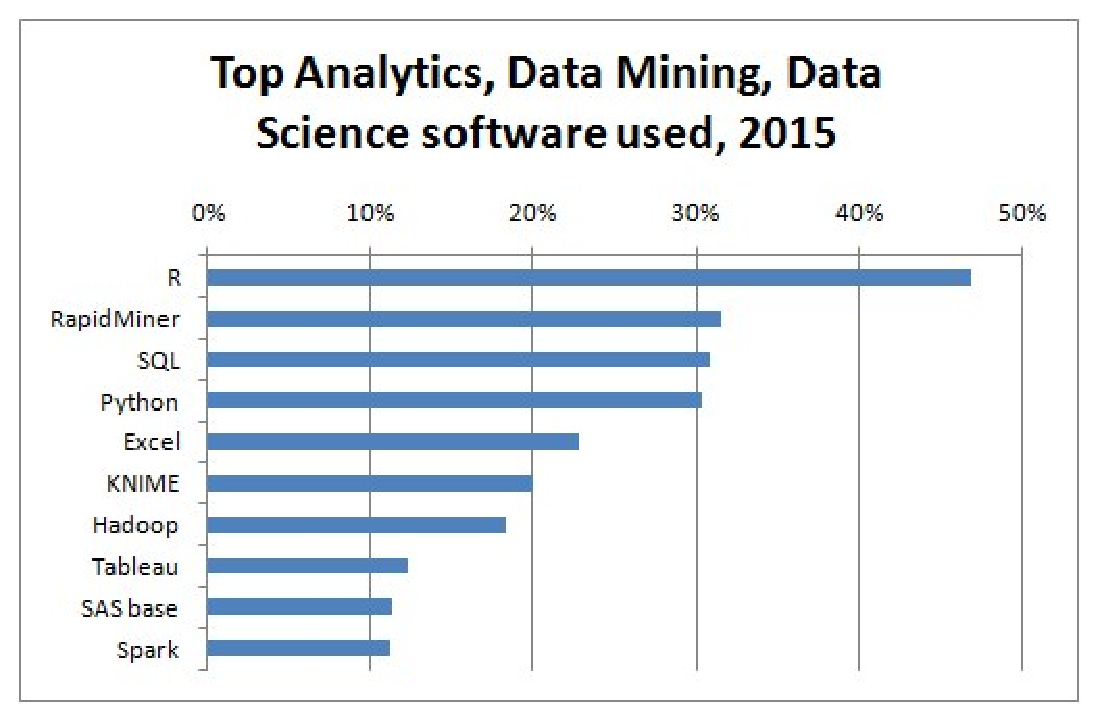
\includegraphics[width=\textwidth]{languages.eps}
\caption[Top analytical tools for data science]{\small \linespread{1.1} Top analytical tools for data science (source: \protect\url{https://www.kdnuggets.com/2015/05/poll-r-rapidminer-python-big-data-spark.html}).} \label{languages}
\end{figure}

We have implemented our proposed methods in 5 different R packages as follows:

\begin{itemize}
\item {\tt{fastCS}}: implements various methods proposed for estimating clustered data with a covariance matrix with compound-symmetry structure.

\item {\tt{fastAR1}}: implements various methods proposed for estimating clustered data with a covariance matrix with AR(1) structure.

\item {\tt{miscVSS}}: implements various methods to perform vertical sample splitting. That includes both random and structured version of this approach.

\item {\tt{imi}}: implements the iterative multiple imputation technique.

\item {\tt{mifa}}: implements our proposal for explanatory factor analysis for incomplete data using multiple imputations.

\end{itemize}

The source codes for all of these R packages are publicly and freely available via author's github page (\url{https://github.com/vahidnassiri}), and can easily be installed from there using the command {\t{install\_git}} which is available via R package {\tt{devtools}}. Therefore, one needs to first install this R package using the following command:

\begin{Shaded}
\begin{Highlighting}[]
\KeywordTok{install.packages}\NormalTok{(}\StringTok{"devtools"}\NormalTok{)}
\end{Highlighting}
\end{Shaded}

Once {\tt{devtools}} is installed, one can use the following command to install any of these packages directly from R environment. Some of the packages are dependent on other R packages. Such dependencies can also be installed automatically in case they user does not already have them installed. 




\section{R package {\tt{fastCS}}}

The R package {\tt{fastCS}} provides functions to:

\begin{itemize}
\item Estimate parameters of balanced clustered data with CS structure covariance matrix 
\item Combine estimated and their variance from different splits using:
\vspace{-\topsep}
\begin{itemize}
\item parameter-free weights
\item scalar weights
\item optimal weights
\end{itemize}
\vspace{-\topsep}
\item Perform cluster by cluster analysis
\end{itemize}

This covers our contributions in Section~\ref{sec_cs}.

\section{R package {\tt{fastAR1}}}

The R package {\tt{fastAR1}} provides function to:

\begin{itemize}
\item Estimate parameters of balanced clustered data with AR1 covariance matrix
\item Estimate variance of the estimates above
\item Combine estimated parameters and their variances from different splits.
\end{itemize}

\section{R package {\tt{miscVSS}}}

The R package {\tt{miscVSS}} provides function to:

\begin{itemize}
\item Perform random vertical splitting using iterative multiple outputation with acceleration
\item Prepare data for structured vertical splitting
\item Combine the estimated parameters and variances from vertical splitting using appropriate combination rules.
\end{itemize}

This covers our contributions in Chapters~\ref{chap_random_vertical}, and \ref{chap_structured_vertical}.


\section{R package {\tt{imi}}}
The R package {\tt{imi}} provides function to:

\begin{itemize}
\item Impute incomplete data and determine the number of sufficient imputed datasets using iterative multiple imputation idea for:
\vspace{-\topsep}
\begin{itemize}
\item Linear models
\item Generalized linear models
\item Student's $t$-test
\end{itemize}
\vspace{-\topsep}
\item Study the convergence of the procedure for a given number of imputed datasets
\item Visualize the convergence procedure and obtained results
\item Combine estimates and covariance matrices from multiple imputation using appropriate rules.
\end{itemize}

This covers our contributions in Section~\ref{secc_IMI}.



\section{R package {\tt{mifa}}}


The R package {\tt{mifa}} provides function to:

\begin{itemize}
\item Impute the incomplete data, determine the number of sufficient imputed datasets, and perform exploratory factor analysis on them.
\item Compute confidence interval for the proportion of explained variance for given numbers of factors using Fieller's method \citep{fieller1954}.
\item Compute confidence interval for the proportion of explained variance for given numbers of factors using bootstrap.
\item Combine estimates and covariance matrices from multiple imputation using appropriate rules.
\end{itemize}

This covers our contributions in Section~\ref{secc_mifa}.

\chapter{Conclusions}

begin with the two promises we made and expalin how they are kept. Given an example of a situation where every thing is there together, 

\begin{itemize}
\item very large sample size
\item highly unbalanced
\item many responses
\item each of very large size
\end{itemize}

so we first split horizontally and structured to put all clusters of the same size together, but still from some sizes we might have too many, so we can split those horizontally by randomly. Then we split structured vertically to do the pairsie approach. but then for some pairs the cluster sizes could be too large which then we split randmly byt vertically. ccombination rules will be applied step by step. Find those steps and mention them. From inner splitting to outer. For example, if we 1- split structured horizontal, 2- random horizontal, we first combine the random horizontals, then the results are combined structred horizontal. 



\chapter{Appendices}

\backmatter

\appendix
\setcounter{equation}{0}
\renewcommand{\theequation}{A.\arabic{equation}}
\renewcommand{\thesection}{A.\arabic{section}}

%% CS paper


\section{Incompleteness in the Compound-symmetry Model} \label{appA}


{Based on (4.1)
%(\ref{driestats}) 
and the multiplicity of the cluster sizes, the sufficient statistics are:
\begin{eqnarray}
W_{1k}&=&\sum_{i=1}^{c_k}\sum_{j=1}^{n_k}Y_{ij}^{(k)},\label{keen}\\
W_2&=&\sum_{k=1}^L\sum_{i=1}^{c_k}\sum_{j=1}^{n_k}\left(Y_{ij}^{(k)}\right)^2,\label{ktwee}\\
W_{3k}&=&\sum_{i=1}^{c_k}\left(\sum_{j=1}^{n_k}Y_{ij}^{(k)}\right)^2,\label{kdrie}\\
W_{4k}&=&c_k.\label{kvier}
\end{eqnarray}
The conditional and marginal expectations of (\ref{keen})--(\ref{kvier}) are:
\[
\begin{aligned}
E(W_{1k}|c_k)&=&c_k n_k\mu,\\
E(W_{1k})&=&N\mu\pi_k n_k,\\
E(W_{2}|c_k)&=&\sum_{k=1}^Lc_k n_k(\sigma^2+d+\mu^2),\\
E(W_{2})&=&N(\sigma^2+d+\mu^2)\sum_{k=1}^L\pi_k n_k,\\
E(W_{3k}|c_k)&=&c_k\left\{
n_k(\sigma^2+d+\mu^2)+n_k(n_k-1)(d+\mu^2)\right\},\\
E(W_{3k})&=&N\pi_k n_k
\left\{
(\sigma^2+d+\mu^2)+(n_k-1)(d+\mu^2)
\right\}
,\\
E(W_{4k})&=&N\pi_k.
\end{aligned}
\]
Group all sufficient statistics in $\BW$ and define a function
\begin{equation}
\label{gcluster}
g(\bw)=\sum_{k=1}^L\lambda_k\frac{w_{1k}}{w_{4k}}.
\end{equation}
Then,
$$E\left\{g(\BW|\BW_4)\right\}=
\sum_{k=1}^L\lambda_k\frac{E(W_{1k}|W_{4k})}{W_{4k}}=
\mu\sum_{k=1}^L\lambda_k n_k,
$$
and hence
$$E\left\{g(\BW)\right\}=
\mu\sum_{k=1}^K\lambda_k n_k.$$
Thus, every solution $\bflambda \perp \bn$, where $\bn=(n_1,\dots,n_K)'$, provides a counterexample, establishing incompleteness.

Such a vector $\bflambda$ exists if and only if $K\ge 2$, for which it is assumed that at least two $c_k>0$ (i.e., at least two different cluster sizes occur).


\section{Likelihood-based Estimation of the CS Model}
\label{likelihoodapp}

\subsection{Score Functions}

The score function has components:
\begin{eqnarray}
\frac{\partial \ell}{\partial \mu_k} & =&
\frac{1}{\sigma_k^2+n_kd_k} \left( \sum_{i=1}^{c_k} \sum_{j=1}^{n_1} y_{ij}^{(k)}-c_k n_k \mu_k\right) ,
\label{jscore1} \\
\frac{\partial \ell}{\partial \sigma_k^2} & =&
 \frac{-c_kn_k}{2\sigma_k^2} \cdot \frac{\sigma_k^2+(n_k-1)d_k}{\sigma_k^2+n_k d_k} + \frac{c_kn_kS_k}{2\sigma_k^4}  \\
 &&-\frac{d_k(2\sigma_k^2+n_kd_k) c_kn_kT_k}{2\sigma_k^4(\sigma_k^2+n_kd_k)^2} ,
\label{jscore2}\\
\frac{\partial \ell}{\partial d_k} & = &
\frac{-c_kn_k}{2(\sigma_k^2+n_kd_k)}+\frac{c_kn_k T_k}{2(\sigma_k^2+n_kd_k)^2},
 \label{jscore3}
\end{eqnarray}
with
\begin{eqnarray}
\label{skfunc}\label{qkfunc}
S_k & =& \frac{1}{c_{kn_k}} Q_k= \frac{1}{c_kn_k}\sum_{i=1}^{c_k} \BZ_i^{(k)'}\BZ_i^{(k)}, \\
\label{tkfunc}\label{rkfunc}
T_k & =&\frac{1}{c_{kn_k}}R_k= \frac{1}{c_{kn_k}}\sum_{i=1}^{c_k} \BZ_i^{(k)'}\mathbf{J_{n_k}}\BZ_i^{(k)}.
\end{eqnarray}



\subsection{Lack of Closed-form Solution when $K\ge 2$}
\label{twodifferent}

The lack of a closed form when $K\ge 2$ is well known, but we highlight a few relevant features here. More detail is given in Supplementary Materials~\ref{appB}.
Function (4.4)
%(\ref{jloglik}) 
can be turned into the log-likelihood kernel for the conventional situation where there is a common mean parameter and common variance components across all cluster sizes, i.e., $\ell(\mu,\sigma^2,d)$. The score functions follow from summing the terms in (\ref{jscore1})--(\ref{jscore3}) across cluster sizes:
\begin{equation}
\label{jscorelik}
\frac{\partial \ell}{\partial \mu}=
\sum_{k=1}^K\left.\frac{\partial \ell}{\partial \mu_k}\right|_{\mu_k=\mu},\qquad
\frac{\partial \ell}{\partial \sigma^2}=
\sum_{k=1}^K\left.\frac{\partial \ell}{\partial \sigma^2_k}\right|_{\sigma^2_k=\sigma^2},
\qquad
\frac{\partial \ell}{\partial d}=
\sum_{k=1}^K\left.\frac{\partial \ell}{\partial d_k}\right|_{d_k=d}.
\end{equation}
Solving the score equation in (\ref{jscorelik}) for the mean, using that
$$\Sigma_{n_k}^{-1}=\frac{1}{\sigma^2}I_{n_k}-\frac{d}{\sigma^2(\sigma^2+n_kd)}J_{n_k},$$
leads to the identity:
\begin{equation}
\widehat{\mu}=\frac
{
\sum_{k=1}^K\frac{n_k c_k}{\sigma^2+n_k d} \overline{Y}^{(k)}
}
{
\sum_{k=1}^K\frac{n_k c_k}{\sigma^2+n_k d}
}
=
\frac
{
\sum_{k=1}^K\frac{n_k c_k}{\sigma^2+n_k d} \widehat{\mu_k}
}
{
\sum_{k=1}^K\frac{n_k c_k}{\sigma^2+n_k d}
},
\label{mulikapp}
\end{equation}
where $\widehat{\mu_k}$ as in (4.5).
%(\ref{muk}).
For the variance components, only implicit identities follow; they are functions of (\ref{skfunc})--(\ref{tkfunc}). These take the form of high-degree polynomials, for which no general explicit solution exists.  While (\ref{mulikapp}) is explicit, it is a weighted average of the cluster-size specific averages $\overline{Y}^{(k)}$, with weights depending on the variance components.  This, combined with the result for the variance components, implies that there is no explicit solution, unless the variance components are known or the cluster size is constant.


\section{Full Likelihood}
 \label{appB}

Referring to the conventional situations, i.e. $\ell(\mu,\sigma^2,d)$ in (4.2)
%(\ref{loglikcs}) 
and the score equation in (\ref{jscorelik}), also second derivatives can be calculated:


\begin{equation}
\frac{\partial^2\ell}{\partial \mu^2}  = \sum_{k=1}^K\frac{-c_kn_k}{\sigma^2+n_kd} \label{jhessian1}
\end{equation}
\begin{equation}
\frac{\partial^2\ell}{\partial \sigma^2 \partial \mu}  = \sum_{k=1}^K \frac{-1}{(\sigma^2+n_kd)^2} \left( \sum_{i=1}^{c_k} \sum_{j=1}^{n_k} y_{ij}^{(k)}-c_k n_k \mu_k\right) \label{jhessian2}
\end{equation}
\begin{equation}
\frac{\partial^2\ell}{\partial d \partial \mu_k}  = \sum_{k=1}^K\frac{-n_k}{(\sigma^2+n_kd)^2} \left( \sum_{i=1}^{c_k} \sum_{j=1}^{n_k} y_{ij}^{(k)}-c_k n_k \mu_k\right) \label{jhessian3}
\end{equation}
\begin{equation}
\frac{\partial^2\ell}{\partial \mu \partial \sigma^2} = \sum_{k=1}^K \left(\frac{-1}{\sigma^4} + \frac{d(2\sigma^2+n_kd)n_k}{\sigma^4(\sigma^2+n_kd)^2} \right) \sum_{i=1}^{c_k}\sum_{j=1}^{n_k}Z_{ij}^{(k)} \label{jhessian4} 
\end{equation}

\begin{multline}
\frac{\partial^2\ell}{(\partial \sigma^2)^2} = \sum_{k=1}^K\left( \frac{c_kn_k}{2\sigma^4} \cdot \frac{\sigma^2+(n_k-1)d}{\sigma^2+n_kd}- \frac{c_kn_k}{2\sigma^2} \cdot \frac{d}{(\sigma^2+n_kd)^2} - \frac{c_kn_k S_k}{\sigma^6} \right. \\
 \left.- d c_kn_kT_k \frac{\sigma^2(\sigma^2+n_kd)-(2\sigma^2+n_kd)^2}{\sigma^6(\sigma^2+n_kd)^3}\right) \label{jhessian5}
\end{multline}

\begin{equation}
\frac{\partial^2\ell}{\partial d \partial \sigma^2} = \sum_{i=1}^K\left( \frac{c_kn_k}{2(\sigma^2+n_kd)}- \frac{c_kn_k T_k}{\sigma^4} \cdot \frac{(\sigma^2+n_kd)^2 - n_k d (2\sigma^2+n_kd)}{(\sigma^2+n_kd)^3} \right)\label{jhessian6}
\end{equation}

\begin{equation}
\frac{\partial^2\ell}{\partial \mu \partial d} =\sum_{k=1}^K \frac{-n_k}{(\sigma^2+n_kd)^2}\sum_{i=1}^{c_k} \sum_{j=1}^{n_k} Z_{ij}^{(k)} \label{jhessian7}
\end{equation}

\begin{equation}
\frac{\partial^2\ell}{\partial \sigma^2 \partial d} = \sum_{k=1}^K\left( \frac{c_kn_k}{2(\sigma^2+n_kd)^2}-\frac{c_kn_kT_k}{(\sigma^2+n_kd)^3} \right) \label{jhessian8}
\end{equation}

\begin{equation}
\frac{\partial^2\ell}{\partial d^2} = \sum_{k=1}^K \left(\frac{c_kn_k^2}{2(\sigma^2+n_kd)^2}-\frac{c_kn_k^2T_k}{(\sigma^2+n_kd)^3} \right) \label{jhessian9} 
\end{equation}






Should we use conditional likelihood, then the log-likelihood's kernel equals:
\begin{multline}
L  \propto \prod^k_{i=1} \frac{1}{(2\pi)^{n_1/2}|\Sigma_{n_1}|^{1/2}} \exp \left\{ -\frac{1}{2}(\by_{i1}-\bmu_{n_1})'\Sigma_{n_1}^{-1} (\by_{i1}-\bmu_{n_1}) \right\}  \\
\times \left[ \frac{\Phi (\alpha + \by'_{i1} \bfbeta)}{\Phi\left( \frac{\alpha + \bmu_{n_1}'\bfbeta}{\sqrt{1+\bfbeta'\Sigma_{n_1}\bfbeta/n_1}} \right)} \right] \\
\times \prod^N_{i=k+1} \frac{1}{(2\pi)^{n_2/2}|\Sigma_{n_2}|^{1/2}}\exp \left\{ -\frac{1}{2}(\by_i-\bmu_{n_2})'\Sigma_{n_2}^{-1} (\by_i-\bmu_{n_2}) \right\} \\
\qquad\times\left[ \frac{1-\Phi (\alpha + \by'_{i1} \bfbeta)}{1-\Phi\left( \frac{\alpha + \bmu_{n_1}'\bfbeta}{\sqrt{1+\bfbeta'\Sigma_{n_1}\bfbeta/n_1}} \right)} \right] \label{clik} 
\end{multline}

\begin{multline}
\ell  \propto - \frac{1}{2} \sum_{i=1}^k \left\{ \ln|\Sigma_{n_1}| + (\by_{i}-\bmu_{n_1})'\Sigma_{n_1}^{-1} (\by_{i1}-\bmu_{n_1}) \right\}  \\
 - k \ln \Phi(\tilde{\alpha} + \bmu_{n_1}'\tilde{\bfbeta})  \\
 -\frac{1}{2} \sum_{i=k+1}^N \left\{ \ln|\Sigma_{n_2}| + (\by_i-\bmu_{n_2})'\Sigma_{n_2}^{-1} (\by_i-\bmu_{n_2}) \right\}\\
 -(N-k) \ln \left\{1-\Phi(\tilde{\alpha} + \bmu_{n_1}' \tilde{\bfbeta})\right\},  \label{cloglik} 
\end{multline}
with $\tilde{\alpha}=\frac{\alpha}{\sqrt{1+\bfbeta'\Sigma_{n_1}\bfbeta/n_1}}$ and  $\tilde{\bfbeta}=\frac{\bfbeta}{\sqrt{1+\bfbeta'\Sigma_{n_1}\bfbeta/n_1}}$

The corresponding score equations are:
\begin{equation}
\begin{aligned}
\frac{\partial\ell}{\partial \mu} & =&\frac{1}{\sigma^2+n_1d} \left( \sum_{i=1}^k \sum_{j=1}^{n_1} \by_{ij}-k n_1 \mu\right)
 - k n_1 \mathbf{j_{n_1}'} \tilde{\bfbeta} \frac{\phi(\tilde{\alpha}+\bmu_{n_1}'\tilde{\bfbeta})}{\Phi(\tilde{\alpha}+\bmu_{n_1}'\tilde{\bfbeta})}  \\
&& + \frac{1}{\sigma^2+n_2d} \left( \sum_{i=k+1}^N \sum_{j=1}^{n_2} \by_{ij}-(N-k) n_2 \mu\right) \\
 &&- (N-k) n_2 \mathbf{j_{n_1}'} \tilde{\bfbeta} \frac{\phi(\tilde{\alpha}+\bmu_{n_1}'\tilde{\bfbeta})}{\Phi(\tilde{\alpha}+\bmu_{n_1}'\tilde{\bfbeta})} \label{cscore1} ,
\end{aligned}
\end{equation}
with $\frac{\partial\ell}{\partial \sigma^2}$ and $\frac{\partial\ell}{\partial d}$ identical to (\ref{jscore2}) and (\ref{jscore3}). The components of the Hessian are:


\begin{equation}
\begin{aligned}
\frac{\partial^2\ell}{\partial \mu^2} & = &\frac{-kn_1}{\sigma^2+n_1d}-\frac{(N-k)n_2}{\sigma^2 +n_2d}  \\
&& - kn_1 \mathbf{j_{n_1}'}\tilde{\bfbeta}\left[ \frac{-\Phi(\tilde{\alpha}+\bmu_{n_1}'\tilde{\bfbeta}) \cdot \phi(\tilde{\alpha}+\bmu_{n_1}'\tilde{\bfbeta})\cdot(\tilde{\alpha}+\bmu_{n_1}'\tilde{\bfbeta}) \cdot \mathbf{j_{n_1}'}\tilde{\bfbeta}}{\Phi^2(\tilde{\alpha}+\bmu_{n_1}'\tilde{\bfbeta})} \right.  \\
&& \left. - \frac{\phi^2(\tilde{\alpha}+\bmu_{n_1}'\tilde{\bfbeta}) \cdot \mathbf{j_{n_1}'}\tilde{\bfbeta}}{\Phi^2(\tilde{\alpha}+\bmu_{n_1}'\tilde{\bfbeta})}\right]  \\
&& +(N-k)n_2 \mathbf{j_{n_1}'}\tilde{\bfbeta}\\
&&\times \left[ \frac{-(1-\Phi(\tilde{\alpha}+\bmu_{n_1}'\tilde{\bfbeta})) \cdot \phi(\tilde{\alpha}+\bmu_{n_1}'\tilde{\bfbeta})\cdot(\tilde{\alpha}+\bmu_{n_1}'\tilde{\bfbeta}) \cdot \mathbf{j_{n_1}'}\tilde{\bfbeta}}{(1-\Phi(\tilde{\alpha}+\bmu_{n_1}'\tilde{\bfbeta}))^2} \right.  \\ 
&& + \left. \frac{\phi^2(\tilde{\alpha}+\bmu_{n_1}'\tilde{\bfbeta}) \cdot \mathbf{j_{n_1}'}\tilde{\bfbeta}}{(1-\Phi(\tilde{\alpha}+\bmu_{n_1}'\tilde{\bfbeta}))^2}\right]\label{chessian1}
\end{aligned}
\end{equation}

\begin{equation}
\begin{aligned}
\frac{\partial^2\ell}{\partial \sigma^2 \partial \mu} & = &\frac{-1}{(\sigma^2+n_1d)^2} \left( \sum_{i=1}^k \sum_{j=1}^{n_1} \by_{ij}-k n_1 \mu\right) \\
&& - \frac{1}{(\sigma^2+n_2d)^2} \left( \sum_{i=k+1}^N \sum_{j=1}^{n_2} \by_{ij}-(N-k) n_2 \mu\right) \label{chessian2} 
\end{aligned}
\end{equation}

\begin{equation}
\begin{aligned}
\frac{\partial^2\ell}{\partial d \partial \mu} & =& \frac{-n_1}{(\sigma^2+n_1d)^2} \left( \sum_{i=1}^k \sum_{j=1}^{n_1} \by_{ij}-k n_1 \mu\right) \\
& &- \frac{n_2}{(\sigma^2+n_2d)^2} \left( \sum_{i=k+1}^N \sum_{j=1}^{n_2} \by_{ij}-(N-k) n_2 \mu\right) \label{chessian3}
\end{aligned}
\end{equation}

with $\frac{\partial^2\ell}{\partial \mu \partial \sigma^2}$, $\frac{\partial^2\ell}{(\partial \sigma^2)^2}$, $\frac{\partial^2\ell}{\partial d \partial \sigma^2}$, $\frac{\partial^2\ell}{\partial \mu \partial d}$, $\frac{\partial^2\ell}{\partial \sigma^2 \partial d}$, and $\frac{\partial^2\ell}{\partial (d)^2}$ indentical to (\ref{jhessian4}),
(\ref{jhessian5}), (\ref{jhessian6}), (\ref{jhessian7}), (\ref{jhessian8}), and (\ref{jhessian9}).

\section{Pseudo-likelihood for Split Samples}
\label{splitsample}

\subsection{General Considerations}
Informally, a pseudo-likelihood function is one that replaces a computationally intractable or slow-to-maximize likelihood function, with another function that still produces a consistent and asymptotically normal estimator when maximised, i.e., by setting the first derivatives of the log pseudo-likelihood equal to zero and solving the resultant pseudo score equations. An early reference is \cite{arnold1991}, and details on various forms of pseudo-likelihood can be found in \cite[Ch.~9, 12, 21, 22, 24, and 25]{molenberghs2005}. In the current clustered setting, the likelihood contribution of a cluster is often replaced by a product of contributions for various sub-vectors. In some cases, such a sub-vector can be conditioned upon another sub-vector.

\cite{Verbeke2006} and \cite{Fetal06} used pseudo-likelihood to fit mixed models to high-dimensional multivariate longitudinal data. They supplemented the standard method with an additional device. They first replaced a set of $M$ longitudinal sequences by the $M(M-1)/2$ longitudinal pairs. This in itself is a standard application of pseudo-likelihood. They then assumed that each pair has its own parameter vector.
Symbolically, this can be written as:
\begin{equation}
p\ell({\bm{\theta}})  \equiv  p\ell(\mathbf{y}_{1i}, \mathbf{y}_{2i}, \ldots, \mathbf{y}_{Mi} |{\bm{\theta}})
 =  \sum_{r<s} \ell(\mathbf{y}_{ri}, \mathbf{y}_{si} | \bm{\theta}_{rs}), \label{mv23 eqn pseudo lik}
\end{equation}
where $\BY_{ri}$ is the $r$th sequence for subject~$i$. In (\ref{mv23 eqn pseudo lik}), $\bm{\theta}$ results from stacking all $M(M-1)/2$ pair-specific parameter vectors $\bm{\theta}_{rs}$. The actual parameter vector of interest is  $\bm{\theta}^*$, the set of non-redundant parameters is $\bm{\theta}$.

To obtain $\bm{\theta}^*$, \cite{Verbeke2006} take averages of all available estimates for that specific parameter, implying that $\mathbf{\widehat{\theta}^*} = A \mathbf{\widehat{\theta}}$ for an appropriate linear combination matrix $A$. Further, combining this step with general pseudo-likelihood inference, a sandwich estimator is used:
\begin{equation}
\sqrt{N}(\mathbf{\widehat{\theta}^*}- \mathbf{\theta^*} )   =  \sqrt{N}(A\widehat{\bm{\theta}}- A \\bm{\theta}) \stackrel{\mbox{\tiny approx.}}{\sim}  N(\mathbf{0}, A I_0^{-1}I_1 I_0^{-1} A'), \label{mv23 distr psister}
\end{equation}
where
\begin{equation}
I_0(\bftheta)=E\left[\frac{\partial^2p\ell(\bftheta)}{\partial\bftheta'\partial\bftheta}\right],\qquad
I_1(\bftheta)=E\left[
\left(\frac{\partial p\ell(\bftheta)}{\partial\bftheta}\right)'.
\frac{\partial p\ell(\bftheta)}{\partial\bftheta}
\right].
\end{equation}


\cite{Iddi2011} took a very similar route to partition a potentially large sample into sub-samples.

To fix ideas, consider log-likelihood (4.4).
%(\ref{jloglik}). 
When used as an instrument to estimate a single vector $(\mu,\sigma^2,d)$, this function can be viewed a pseudo-likelihood. This setting can be generalized by assuming that a dataset, consisting of repeated measures per subject, is divided into $K$ subgroups, each containing $c_k$ independent replicates. Consider the pseudo-likelihood:
\begin{equation}
\label{ourgenpl}
p\ell(\bftheta)=\sum_{k=1}^K\ell(\bftheta_k|\by_1^{(k)},\dots,\by_{c_k}^{(k)}).
\end{equation}
While the underlying principle is similar to (\ref{mv23 eqn pseudo lik}), it 
is not identical. The similarities are: (1) all $\bftheta_k$ are assumed to 
be different, allowing for separate, even parallel, estimation; (2) 
$\bftheta$ stacks all vectors $\bftheta_k$; (3) the parameter of 
interest $\bftheta^\ast$, is found from an appropriate combination 
of the $\bftheta_k$. Parallel estimation was also followed 
by \cite{scott2016bayes} and \cite{neiswanger2013asymptotically}.



\begin{sloppypar}
There are important differences, however. Here, and in the remainder 
of the article, we assume that
$\ell(\bftheta_k|\by_1^{(k)},\dots,\by_{c_k}^{(k)})$ is the likelihood 
that we would have, should group $k$ be the only one in the data. 
That is, the individual likelihood contributions are not altered, 
rather the data are partitioned. This is similar to the independent 
partitioning done by \cite{Iddi2011}. In line with their derivations, 
(\ref{mv23 distr psister}) can also be used here. Given that 
$\ell_k(\bftheta_k)$ is a genuine likelihood, its contributions 
to $I_0(\bftheta)$ and $I_1(\bftheta)$ are identical, up to the sign. 
As a result, $I_0(\bftheta)^{-1}I_1(\bftheta)I_0(\bftheta)^{-1}=-I_0(\bftheta)^{-1}$, 
a block-diagonal matrix with blocks of the form $I_0(\bftheta_k)$. We now turn to the split-sample case.
\end{sloppypar}



\subsection{Pseudo-likelihood for Split Sample }
\label{appC}


{\cite{Iddi2011}  chose
\begin{equation}
\label{amtrix}
A=\frac{1}{K}(I,\dots,I)
\end{equation}
to pass from $\bftheta$ to $\bftheta^\ast$. This is a sensible choice in the 
i.i.d.\ setting (e.g., when all clusters in a CS model have the same size) 
and with the same number of subjects per sub-sample. The estimator and 
precision estimator then become:
\begin{eqnarray}
\label{schatterindep}
\widehat{\bftheta}^*&=&\frac{1}{K}\sum_{k=1}^K\widehat{\bftheta}_k,\\
\label{asymptoticvarianceexpected}
\mbox{var}(\widehat{\bftheta}^*)&=&\frac{1}{K}H_{\widehat{\theta}}^{-1},
\end{eqnarray}
with $H_{\widehat{\theta}}^{-1}=-I_0(\bftheta_k)$. In this special case, 
the expected information matrices are identical. Alternatively, 
one can use the observed information matrices, and then use instead:
\begin{equation}
\label{asymptoticvarianceobserved}
\frac{1}{K^2}\sum_{k=1}^K{\cal H}_{\widehat{\theta}, k}^{-1}.
\end{equation}
where ${\cal H}_{\widehat{\theta}, k}$ is the observed 
information for sub-sample $k$.

In this particular case, pseudo-likelihood produces the same 
estimator as full likelihood. This stems from the fact that 
all subjects follow the same distribution, in contrast to, 
for example, the setting set out at the start of Section~4.
%\ref{model}. 
Should the subjects have identical distributions, but with $c_k$ variables, 
the above results can be modified accordingly. For example, 
(\ref{schatterindep}) would be replaced by
$$
\widehat{\bftheta}^*=\sum_{k=1}^K\frac{c_k}{N}\widehat{\bftheta}_k,
$$
with similar modification to precision estimation. In this case, 
full likelihood would be obtained.

In the next section, we will consider the more general case where 
different subjects may have a different distribution such as, 
for example, 
the CS case with a different number of measurements 
per cluster.}

\section[Optimal Scalar Weights for CS]{Derivation of Optimal Scalar Weights for Compound-symmetry Case}

To find the optimal scalar weight with minimum variance for $\mu$ we use the method of Lagrange with the constraint that the weights $a_k$ need to sum to 1:
\begin{equation}
Q=\sum_{k=1}^K a_k^2\frac{\sigma^2+n_k d}{c_kn_k}-\lambda\left(\sum_{k=1}^Ka_k-1\right).
\end{equation}
Solving the first partial derivative we become an expression for $a_k$ involving $\lambda$. Summing this one produces an expression for $\lambda$, leading to the complete formula for $a_k$. Precisely, the system of equations is:
\begin{eqnarray}
\frac{\partial Q}{\partial a_k}=2a_k\frac{\sigma^2+n_kd}{c_kn_k}-\lambda&=&0 ,\\
\frac{\partial Q}{\partial \lambda}= \sum_{k=1}^Ka_k-1&=&0,
\end{eqnarray}
or, alternatively:
\begin{eqnarray}
a_k&=&\frac{\lambda}{2}\frac{c_kn_k}{\sigma^2+n_k d},\\
\lambda&=& \left(\frac{1}{2} \sum_{k=1}^K \frac{c_kn_k}{\sigma^2+n_k d}\right)^{-1},
\end{eqnarray}
and hence
$$ a_k= \frac{\frac{c_kn_k}{\sigma^2+n_k d}}{\sum_{m=1}^K\frac{c_m n_m}{\sigma^2+n_m d}}
.$$

In the same manner, expressions for $b_k$ and $g_k$ can be found, as we will show next.
For $\sigma^2$:
$$
Q=2\sigma^4 \sum_{k=1}^K b_k^2\frac{1}{c_k(n_k-1)}-\lambda\left(\sum_{k=1}^Kb_k-1\right),
$$
producing the system:
\begin{eqnarray}
\frac{\partial Q}{\partial b_k}=\frac{4\sigma^4 b_k}{c_k(n_k-1)}-\lambda&=&0, \\
\frac{\partial Q}{\partial \lambda}= \sum_{k=1}^Kb_k-1&=&0,
\end{eqnarray}
which can be rewritten as:
\begin{eqnarray}
4\sigma^4 b_k&=&\lambda c_k (n_k-1),\\
\lambda&=& \frac{4\sigma^4}{\sum_{k=1}^Kc_k(n_k-1)},
\end{eqnarray}
and finally:
$$b_k= \frac{c_k(n_k-1)}{\sum_{m=1}^K c_m(n_m-1)}.
$$
For $d$, the objective function is:
$$
Q=\sum_{k=1}^K g_k^2 v_k-\lambda(\sum_{k=1}^Kg_k-1),
$$
with
$$v_k=\frac{2}{c_kn_k}\left( \frac{\sigma^4}{n_k-1}+2d\sigma^2+n_kd^2\right).$$
The system of equations now is:
\begin{eqnarray}
\frac{\partial Q}{\partial g_k}=2g_k v_k-\lambda&=&0, \\
\frac{\partial Q}{\partial \lambda}= \sum_{k=1}^K g_k-1&=&0,
\end{eqnarray}
leading to:
\begin{eqnarray}
g_k&=&\lambda \frac{1}{2 v_k},\\
\lambda&=& \frac{2}{\sum_{k=1}^K \frac{1}{v_k}},
\end{eqnarray}
giving the solution:
$$ g_k= \frac{\frac{c_kn_k}{\frac{\sigma^4}{n_k-1}+2d\sigma^2+n_kd^2}}{\sum_{m=1}^K\frac{c_m n_k}{n_m-1}+2d\sigma^2+n_md^2}.$$

\subsection{Cluster-by-cluster Analysis}
\label{cbcaapp}

We study the case of the most extreme partitioning, i.e., where each of the clusters is analyzed separately. 
This can be relevant in cases with perhaps a limited number of very to extremely large clusters.  This 
means that $c_k\equiv 1$ throughout. Clearly, the $n_k$ will 
then no longer be unique. We will examine this case in detail, 
and contrast a first weighted estimator with an  
{\em ad hoc\/} one.


\subsubsection{The Weighted Estimator for the Cluster-by-cluster Case}

The estimator follows from setting $c_k\equiv 1$ and hence $K\equiv N$ 
throughout. For example, this special case can easily be considered 
for all expressions in Sections~6.1.1-6.1.3.
%\ref{owcs}--\ref{scalarcs}. 
Because $c_k$ 
enters the inverse of the variance-covariance matrix multiplicatively, as 
is seen from (4.8)-(4.9),
%(\ref{varexprmuk})--(\ref{varexprsigmakdk}), 
the optimal 
estimator that is obtained when each cluster is considered to be its own 
stratum, is identical to the one obtained when strata are defined in 
terms of all clusters of a given size. The same is true for the scalar 
weights.

It is insightful to consider in more detail the special case where 
further the cluster sizes are all identical to $n$. One then easily 
obtains:
\begin{eqnarray}
\label{muconstant}
\widehat{\mu}&=&\frac{1}{Nn}\sum_{i=1}^{N}\sum_{j=1}^{n}Y_{ij},\\[2mm]
\widehat{\sigma}^2&=&\frac{1}{Nn(n-1)}\left(
n\sum_{i=1}^{N}\BZ_{i}'\BZ_{i}-\sum_{i=1}^{N}\BZ_{i}'J_{n}\BZ_{i}
\right)  \\
&=&\frac{1}{Nn(n-1)}(nQ-R),\label{sigmaconstant}\\[2mm]
\widehat{d}&=&
\frac{1}{Nn(n-1)}\left(
\sum_{i=1}^{N}\BZ_{i}'J_{n}\BZ_i-\sum_{i=1}^{N}\BZ_{i}'\BZ_{i}
\right) \\
&=& \frac{1}{Nn(n-1)}(Q-R),\label{dconstant}
\end{eqnarray}
with obvious notation for $Q$ and $R$, inspired by
(\ref{qkfunc})--(\ref{rkfunc}). The corresponding variance-covariance 
elements, similar in spirit to (4.8)-(4.9),
%(\ref{varexprmuk})--(\ref{varexprsigmakdk}), 
are:
\begin{eqnarray}
\label{varexprmucbyc}
\mbox{var}(\widehat{\mu})&=&\frac{\sigma^2+nd}{Nn},\\
\label{varexprsigmadcbyc}
\mbox{var}\left(\begin{array}{c}\widehat{\sigma^2}\\ \widehat{d}\end{array}\right)&=&
\left(
\begin{array}{cc}
\frac{2\sigma^4}{N(n-1)}&-\frac{2\sigma^4}{Nn(n-1)}\\
-\frac{2\sigma^4}{Nn(n-1)}&
\frac{2}{Nn}\left[\frac{\sigma^4}{n-1}+2\sigma^2d+nd^2\right]
\end{array}
\right).
\end{eqnarray}
This estimator coincides with the MLE, as is known from \cite{Iddi2011}.


\subsubsection{A Two-stage Estimator for Compound Symmetry}

In linear mixed models, there is a method of estimation, sometimes called 
the two-stage approach \citep{laird1982random,verbeke2009}, in which each cluster is 
analyzed separately to begin with, using linear regression, after 
which the cluster-specific parameters are summarized into fixed effects. 
Although the above cluster-by-cluster analysis is superficially similar to this,
it is not equivalent. In particular, there is no bias (as can be seen in 
the two stage method), and the maximum likelihood estimator is recovered. 

This approach is most useful when cluster sizes are not constant, 
and in models that are more complex than compound symmetry. However, 
to gain some insight, we develop the details of the method for the CS model 
with constant cluster size.

For the mean, (\ref{muconstant}) is retained, as the average of the 
cluster-specific averages $\overline{Y}_i$. Further, define:
\begin{eqnarray}
\label{twostages1}
s^2&=&\frac{1}{Nn}\sum_{i=1}^N\sum_{j=1}^n(Y_{ij}-\overline{Y}_i)^2,\\
t^2&=&\frac{1}{N}\sum_{i1}^N(\overline{Y}_i-\widehat{\mu})^2.
\label{twostaget1}
\end{eqnarray}
Straightforward algebra shows:
\begin{eqnarray}
\label{exps1}
E(s^2)&=&\frac{n-1}{n}\sigma^2,\\
\label{expt1}
E(t^2)&=&\frac{N-1}{N}\left(d+\frac{1}{n}\sigma^2\right).
\end{eqnarray}
Should $n$ and $N$ approach infinity, then it follows that $s^2$ and $t^2$ 
are asymptotically unbiased estimators for $\sigma^2$ and $d$, 
respectively. However, this is not always reasonable. In applications 
such as the NTP data (Section~2),
%\ref{ntpintro}), 
it is fair to say that 
the cluster size has a biological upper limit. In other situations, 
however, such as meta-analyses, it is sensible to assume that both 
$n$ and $N$ approach infinity.

In the next section, we will study the consequences of removing the bias. 
For now, a small, obvious modification is:
\begin{eqnarray}
\label{twostages2}
s^2_\ast&=&\frac{n}{n-1}s^2,\\
t^2_\ast&=&\frac{N}{N-1}t^2.
\label{twostaget2}
\end{eqnarray}
Now, $s^2_\ast$ is unbiased, while $E(t^2_\ast)=d+\sigma^2/n$, 
the bias $\sigma^2/n$ can be made to disappear asymptotically 
provided it is sensible to let $n$ grow large.

It is of interest to consider the variance-covariance structure 
of the estimators $s^2$, $t^2$, $s^2_\ast$, and $t^2_\ast$, as 
well as to make relative efficiency considerations. This will 
be done next.

\subsubsection{Connections Between Estimators}

Comparing algebraic expressions (\ref{sigmaconstant})--(\ref{dconstant}) 
with (\ref{twostages1})--(\ref{twostaget1}), leads to the linear 
relationships:
\begin{eqnarray}
\label{rel1}
s^2&=&\frac{n-1}{n}\widehat{\sigma^2}+0\cdot\widehat{d},\\
t^2&=&\frac{N-1}{Nn}\widehat{\sigma^2}+\frac{N-1}{N}\widehat{d}.
\label{rel2}
\end{eqnarray}
Relationships (\ref{rel1})--(\ref{rel2}) can be combined with 
(\ref{varexprsigmadcbyc}) to produce:
\begin{equation}
\mbox{var}\left(\begin{array}{c}s^2\\ t^2\end{array}\right)=
\left(
\begin{array}{cc}
\frac{2(n-1)\sigma^4}{Nn^2}&0\\
0&
\frac{2(N-1)^2}{N^2n}\left[\frac{\sigma^4}{n}+2\sigma^2d+nd^2\right]
\end{array}
\right)
\end{equation}
and, similarly,
\begin{equation}
\mbox{var}\left(\begin{array}{c}s^2_\ast\\ t^2_\ast\end{array}\right)=
\left(
\begin{array}{cc}
\frac{2\sigma^4}{N(n-1)}&0\\
0&
\frac{2}{Nn}\left[\frac{\sigma^4}{n}+2\sigma^2d+nd^2\right]
\end{array}
\right).
\end{equation}
From its definition it follows that $s^2_\ast\equiv\widehat{\sigma^2}$. 
The same is not true for $t^2_\ast$. One reason to consider it 
nevertheless is its independence from $s^2_\ast$. Indeed, 
$(\widehat{\mu},s^2_\ast\equiv\widehat{\sigma^2}, t^2_\ast)'$ 
is an estimator with mutually independent components. While the 
same is true when $s^2$ and $t^2$ are used instead, the biases are 
larger.

For this case then, the choice between $\widehat{d}$ and $t^2_\ast$ 
is in terms of a trade-off between efficiency and independence.

To gauge the efficiency loss when using $t^2_\ast$, the mean 
squared error is:
$$MSE(t^2_\ast)=\frac{2}{Nn}\left(\frac{\sigma^4}{n}+2\sigma^2d+nd^2\right)+\frac{1}{n^2}\sigma^4,$$
and hence the relative MSE:
\begin{equation}
\label{releff}
RMSE(t^2;\widehat{d})=\frac
{
2\left(\frac{\sigma^4}{n}+2\sigma^2d+nd^2\right)+\frac{N}{n}\sigma^4
}
{
2\left(\frac{\sigma^4}{n-1}+2\sigma^2d+nd^2\right)
},
\end{equation}
which approaches infinity when $N$ does, while $n$ would 
remain constant. In other words, this estimator is inconsistent 
unless it is being applied in situations where $n$ can also be considered 
to be large.

There are three distinct situations. First, when $N/n=\lambda n+o(n)$, 
for some $\lambda$, i.e., when $N$ is of the order of $n^2$, then, 
based on (\ref{releff}), the ARE is $2(d^2+\lambda\sigma^4)/[2d^2]$. 
The magnitude of the efficiency loss depends on sizes of the parameters involved. 
Second, when ${\cal O}(N)<{\cal O}(n^2)$, the ARE equals~1. This includes 
the cases where $N$ is constant, $N=n^{1/2}$, $N=n$, and $N=n^{3/2}$, for 
example. A constant or slowly increasing $N$ is plausible in a meta-analytic 
context. Third,  if $N/n$ increases too quickly, i.e., 
${\cal O}(N/n)>{\cal O}(n)$, then the estimator $t^2_\ast$ is inconsistent. 
This is the case, in particular, for bounded $n$.

The estimators $s^2$ and $t^2$ can be combined 
linearly to produce unbiased estimators. In other words, 
based on (\ref{exps1})--(\ref{expt1}), the following 
corrections can be applied to (\ref{twostages1})--(\ref{twostaget1}):
\begin{eqnarray}
s^2_{\mbox{\scriptsize corr}}&=&\frac{n}{n-1}s^2,\\
t^2_{\mbox{\scriptsize corr}}&=&\frac{N}{N-1}t^2-\frac{N}{(n-1)(N-1)}s^2.
\end{eqnarray}
Interestingly, this requirement reproduces (\ref{rel1})--(\ref{rel2}): 
the requirement of an unbiased estimator reproduces $\widehat{\sigma^2}$ 
and $\widehat{d}$, presented in
(\ref{sigmaconstant})--(\ref{dconstant}) and hence also with their variance.




\section{Details About the First Simulation Study}
\label{simapp}

The simulation study, summarized in Section~7,
%\ref{simulation}, 
is described in detail here.

\subsection{Simulation Method}

The design of the simulation study is as follows.
\begin{itemize}
\item Each generated set of data consists of $c_k$ clusters of size $n_k$, for $k=1,\dots,K$. We choose $K=4$ throughout.
\item For a generated set of data, the splitting is done by placing all clusters of a given size in one sub-sample.
\item The CS model parameters are $\mu=0$, $d=1$, and $\sigma^2=2$.
\item After estimating the three model parameters within each sub-sample, they are combined using the following weighting methods: (a) equal, (b) proportional, where the weights are
$$w_k=\frac{c_k}{\sum_{\ell=1}^4 c_\ell},$$
and (c) size-proportional, where the weights for $\mu$ and $d$ are:
$$w_k\frac{c_k n_k}{\sum_{\ell=k}^4 c_\ell n_\ell},$$
while for $\sigma^2$ we take:
$$w_k=\frac{c_k (n_k-1)}{\sum_{\ell=1}^4 c_\ell (n_\ell-1)}.$$
\item Per setting, 100 replications are considered.
\end{itemize}
These settings are applied to various combinations of the $n_k$ and $c_k$, now described in turn.




\subsection[Setting 1]{Setting 1: Equal $c_k\cdot n_k$, Different $c_k$ and $n_k$.}

Consider  150 samples in each split, as follows: $(c_1,n_1)=(3,50)$, $(c_2,n_2)=(5,30)$, $(c_3,n_3)=(10,15)$, and $(c_4,n_4)=(15,10)$. The results are presented in Table~\ref{tab150}.  Graphical depictions can be found in Figures~\ref{CS150} and \ref{CS150COMB}. Figure~\ref{CS150} shows that there is a different amount of information in the various sub-samples. This is not a problem, rather a consequence of the way the splits are created and the different amounts of information carried in each. It reminds us that we need to be judicious how the information from the splits will be weighted. It is  not a surprise that equal weights are a poor choice. The other methods perform similarly, and all do very well. To varying degrees, the same will be seen in Settings~2 and~3.
\begin{table}[h]
\caption{\label{tab150}\label{tab150comb} \small \linespread{1.1} First simulation study. Setting 1. Average of split-specific and combined (weighted) parameters and their precision estimates.}

\vspace*{2mm}
\centering
\def\arraystretch{0.6}\begin{tabular}{rrrrrrr}
  \hline\hline
 & \multicolumn{1}{c}{$\mu$} & \multicolumn{1}{c}{\mbox{var}($\mu$)} & \multicolumn{1}{c}{$d$} & \multicolumn{1}{c}{\mbox{var}($d$)} & \multicolumn{1}{c}{$\sigma^2$} & \multicolumn{1}{c}{\mbox{var}($\sigma^2$)} \\
  \hline
split1 & -0.00396 & 0.05779 & 0.68143 & 0.41395 & 1.98676 & 0.00296 \\
  split2 & 0.05697 & 0.03071 & 0.80997 & 0.19712 & 1.98578 & 0.00304 \\
  split3 & -0.02111 & 0.01174 & 0.95161 & 0.07869 & 1.97690 & 0.00319 \\
  split4 & 0.01123 & 0.00626 & 0.98870 & 0.04677 & 1.98056 & 0.00347 \\
   \hline
Equal & 0.01078 & 0.03769 & 0.85793 & 0.09988 & 1.98250 & 0.01406 \\
  Prop & 0.00698 & 0.03230 & 0.92245 & 0.08568 & 1.98081 & 0.01907 \\
  Size prop & 0.01078 & 0.03769 & 0.85793 & 0.09988 & 1.98260 & 0.01405 \\
  Full & 0.00780 & 0.03513 & 0.98016 & 0.08614 & 1.98257 & 0.01392 \\
   \hline
\hline
\end{tabular}
\end{table}


\begin{figure}[!t]
\centering
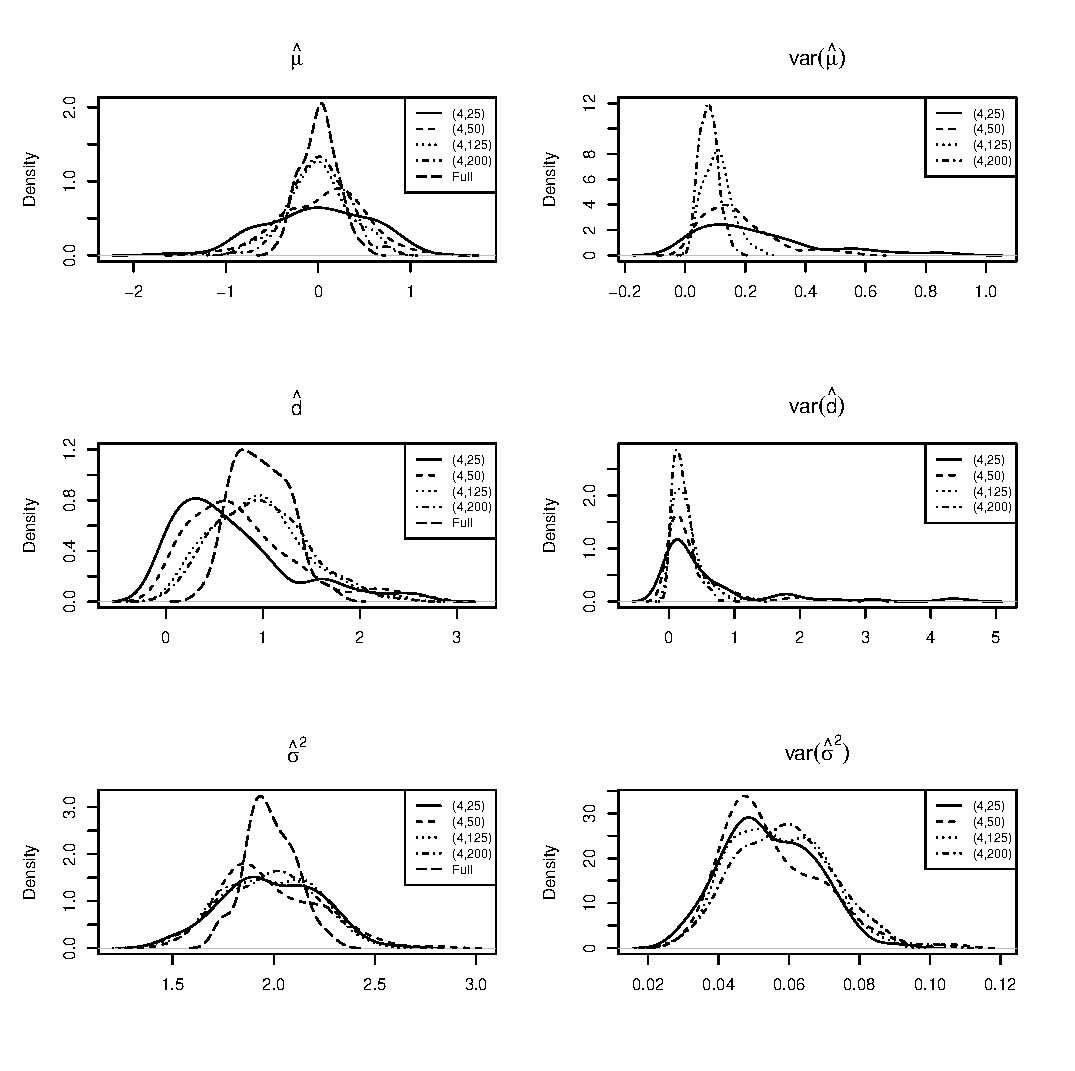
\includegraphics[width=\textwidth]{aCS150.eps}
\caption{\small \linespread{1.1} First simulation study. Setting 1. Split-specific results.} \label{CS150}
\end{figure}
\begin{figure}[!t]
\centering
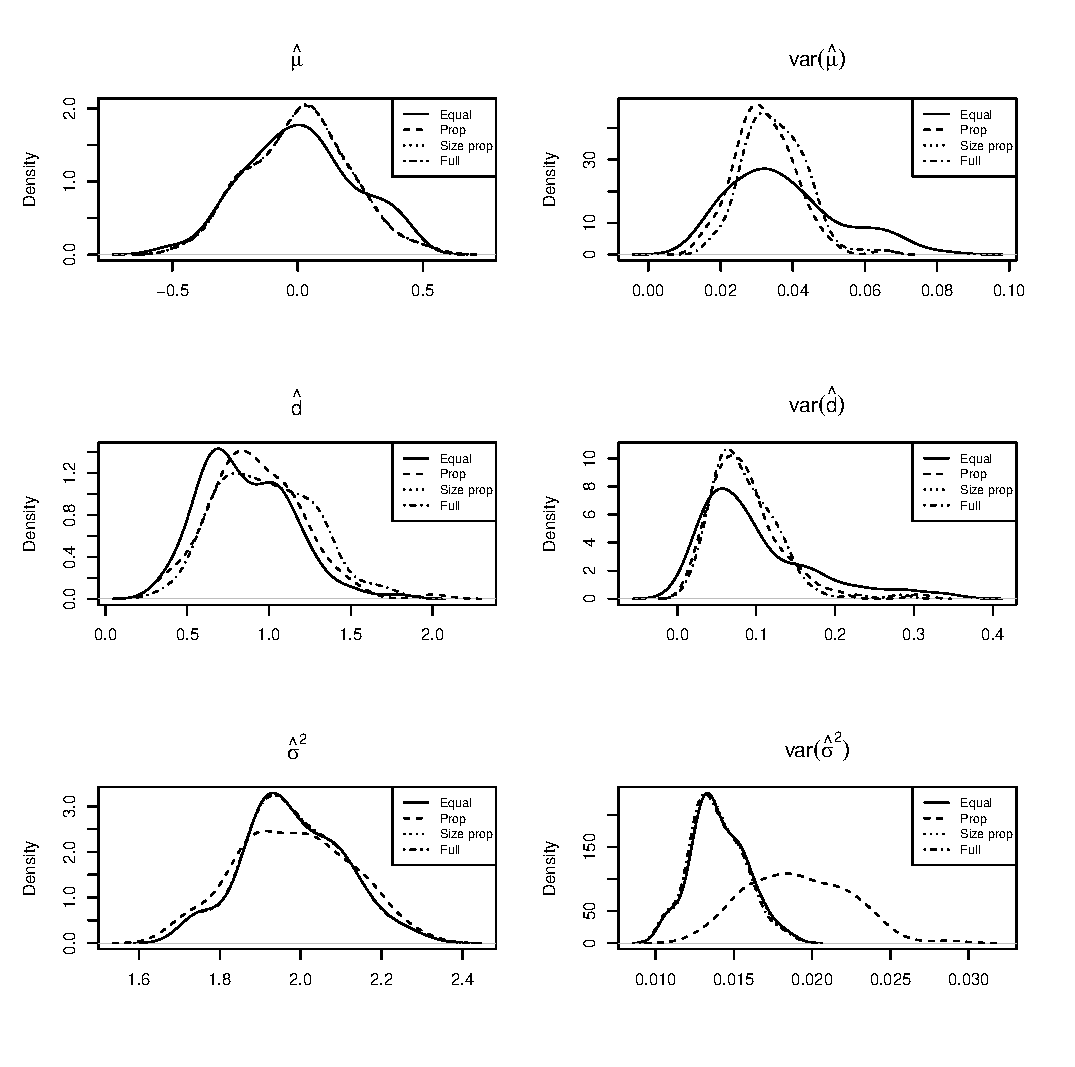
\includegraphics[width=\textwidth]{aCS150COMB.eps}
\caption{\small \linespread{1.1} First simulation study. Setting 1. Combining the results from the four splits, using equal, proportional, and size proportional weights. This is compared with full maximum likelihood.} \label{CS150COMB}
\end{figure}



\subsection[Setting 2]{Setting 2: Different $c_k\cdot n_k$, Equal $c_k$, Different $n_k$}

To see the effect of split size, the following choices are made:
$(c_1,n_1)=(4,25)$,  $(c_2,n_2)=(4,50)$,  $(c_3,n_3)=(4,125)$, and $(c_4,n_4)=(4,250)$.
As a consequence, the size of the splits will be $100$, $200$, $500$, and $1000$, respectively. Table~\ref{tab_diff1} summarized the results, with graphical displays presented in Figures~\ref{CS_diff1} and \ref{CS_diff_comb}.
\begin{table}[t]
\centering
\caption{\small \linespread{1.1} First simulation study. Setting 2. Average of split-specific and combined (weighted) parameters and their precision estimates.}
\label{tab_diff1}

\vspace*{2mm}

\def\arraystretch{0.6} \begin{tabular}{rrrrrrr}
\hline  \hline
  & \multicolumn{1}{c}{$\mu$} & \multicolumn{1}{c}{\mbox{var}($\mu$)} & \multicolumn{1}{c}{$d$} & \multicolumn{1}{c}{\mbox{var}($d$)} & \multicolumn{1}{c}{$\sigma^2$} & \multicolumn{1}{c}{\mbox{var}($\sigma^2$)} \\
\hline
split1 & -0.02515 & 0.05227 & 0.83440 & 0.52423 & 2.00347 & 0.00730 \\
  split2 & 0.01287 & 0.05157 & 0.86891 & 0.57904 & 1.97285 & 0.00160 \\
  split3 & 0.06812 & 0.03586 & 0.74147 & 0.23681 & 2.00165 & 0.00026 \\
  split4 & -0.03676 & 0.02979 & 0.68241 & 0.14117 & 1.99216 & 0.00006 \\
  \hline
 Equal & 0.00477 & 0.05111 & 0.78180 & 0.14770 & 1.99253 & 0.00935 \\
  Prop & 0.00477 & 0.05111 & 0.78180 & 0.14770 & 1.99253 & 0.00935 \\
  Size prop & -0.00147 & 0.07139 & 0.72798 & 0.16585 & 1.99328 & 0.00447 \\
  Full & 0.00530 & 0.06339 & 0.89599 & 0.14604 & 1.99333 & 0.00446 \\
 \hline
\hline
\end{tabular}
\end{table}

\begin{figure}[!t]
\centering
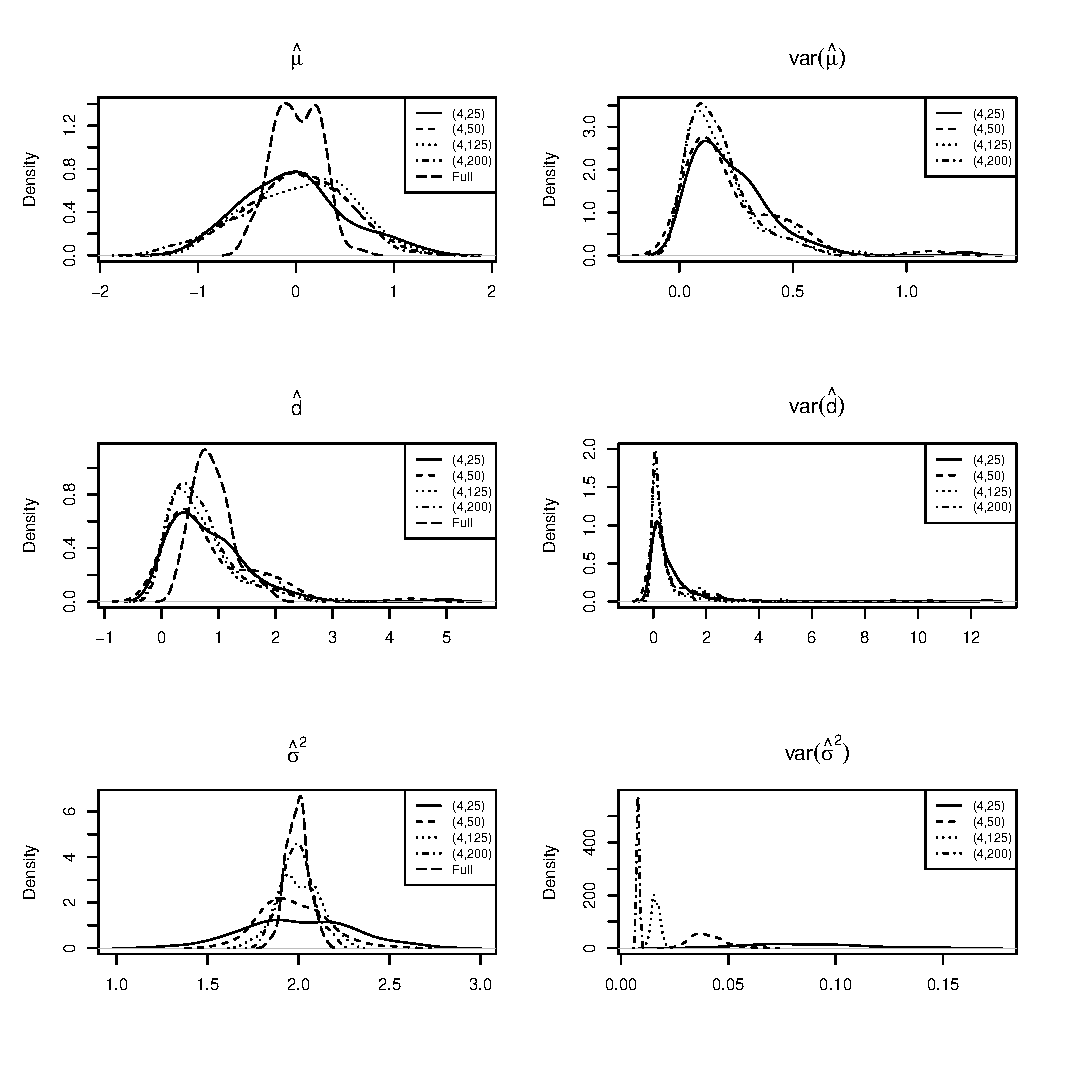
\includegraphics[width=\textwidth]{aCS_diff1.eps}
\caption{\small \linespread{1.1} First simulation study. Setting 2. Split-specific results.} \label{CS_diff1}
\end{figure}
\begin{figure}[!t]
\centering
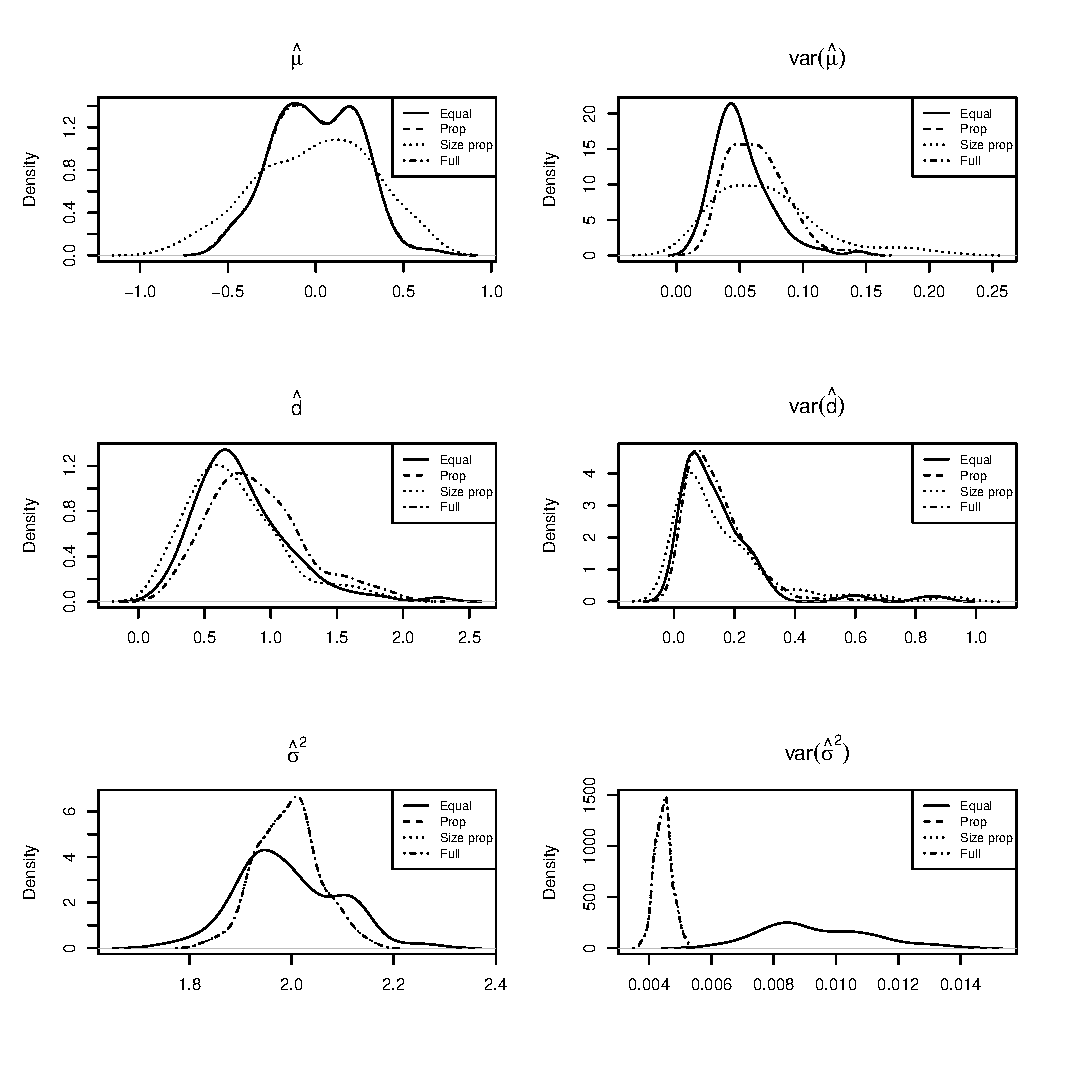
\includegraphics[width=\textwidth]{aCS_diff_comb.eps}
\caption{\small \linespread{1.1} First simulation study. Setting 2. Combining the results from the four splits, using equal, proportional, and size proportional weights. This is compared with full maximum likelihood.} \label{CS_diff_comb}
\end{figure}


\subsection[Setting 3]{Setting 3: Different $c_k\cdot n_k$, Different $c_k$, Equal $n_k$}
We now choose: $(c_1,n_1)=(10,20)$,  $(c_2,n_2)=(20,20)$, $(c_3,n_3)=(50,20)$, and
$(c_4,n_4)=(100,20)$. Table~\ref{tab_diff2} summarizes the results. Graphs can be found in Figures~\ref{CS_diff2} and \ref{CS_diff_comb2}.
\begin{table}[h]
\centering
\caption{\small \linespread{1.1} First simulation study. Setting 3. Average of split-specific and combined (weighted) parameters and their precision estimates.}
\label{tab_diff2}

\vspace*{2mm}

\def\arraystretch{0.6} \begin{tabular}{rrrrrrr}
  \hline\hline
  & \multicolumn{1}{c}{$\mu$} & \multicolumn{1}{c}{\mbox{var}($\mu$)} & \multicolumn{1}{c}{$d$} & \multicolumn{1}{c}{\mbox{var}($d$)} & \multicolumn{1}{c}{$\sigma^2$} & \multicolumn{1}{c}{\mbox{var}($\sigma^2$)} \\
  \hline
split1 & 0.00343 & 0.00900 & 0.84739 & 0.05169 & 2.02445 & 0.00190 \\
  split2 & 0.02553 & 0.00304 & 1.00224 & 0.01754 & 2.01962 & 0.00047 \\
  split3 & -0.00010 & 0.00045 & 0.95794 & 0.00212 & 1.99765 & 0.00007 \\
  split4 & 0.01151 & 0.00012 & 1.01226 & 0.00064 & 1.98944 & 0.00002 \\
   \hline
 \hline
Equal & 0.01009 & 0.01139 & 0.95496 & 0.02694 & 2.00779 & 0.00486 \\
  Prop & 0.00939 & 0.00604 & 0.98690 & 0.01369 & 1.99702 & 0.00234 \\
  Size prop & 0.00939 & 0.00604 & 0.98690 & 0.01369 & 1.99702 & 0.00234 \\
  Full & 0.00939 & 0.00614 & 1.00487 & 0.01372 & 1.99702 & 0.00233 \\
 \hline\hline
\end{tabular}
\end{table}


\begin{figure}[!t]
\centering
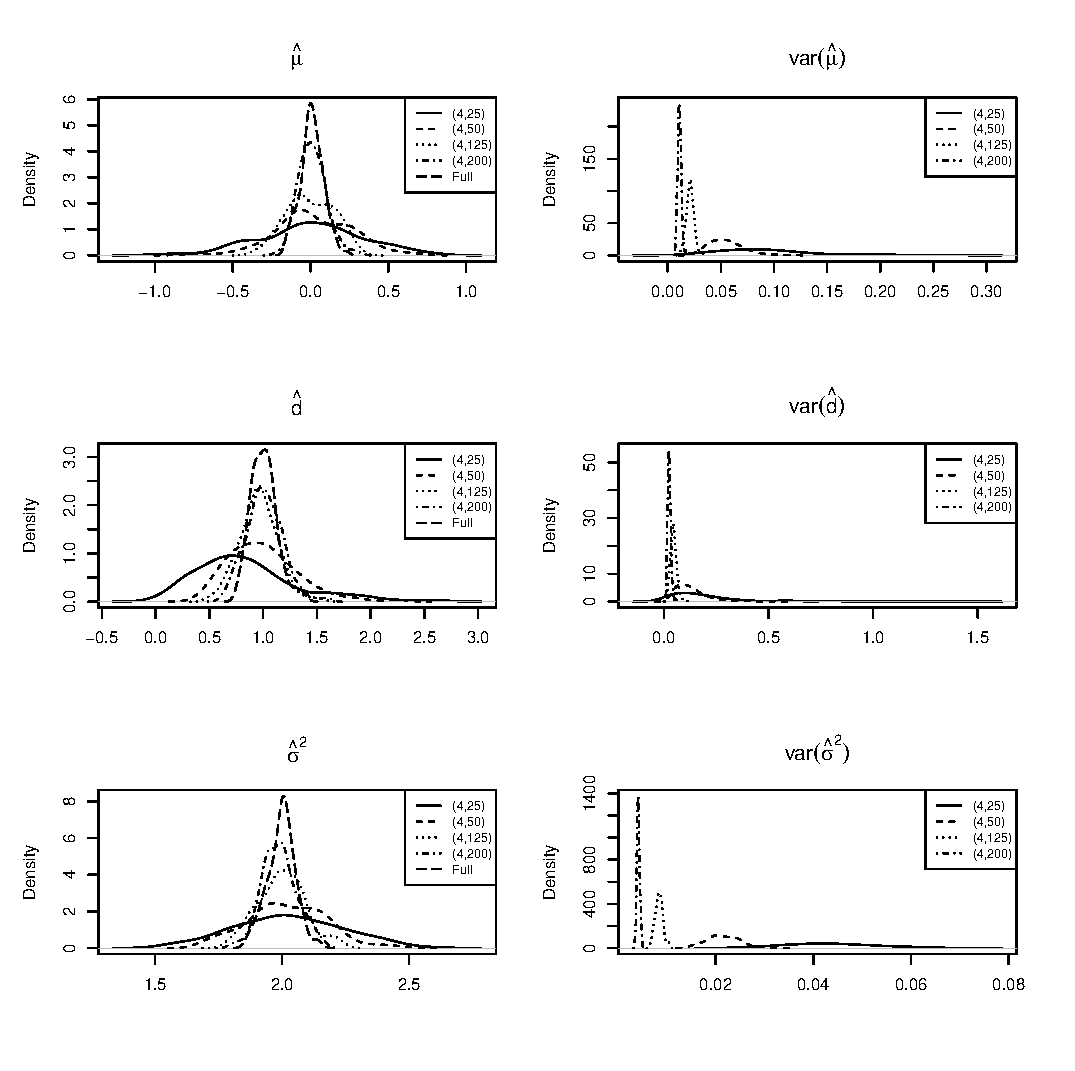
\includegraphics[width=\textwidth]{aCS_diff2.eps}
\caption{\small \linespread{1.1} First simulation study. Setting 3. Split-specific results. \label{CS_diff2}}
\end{figure}
\begin{figure}[!t]
\centering
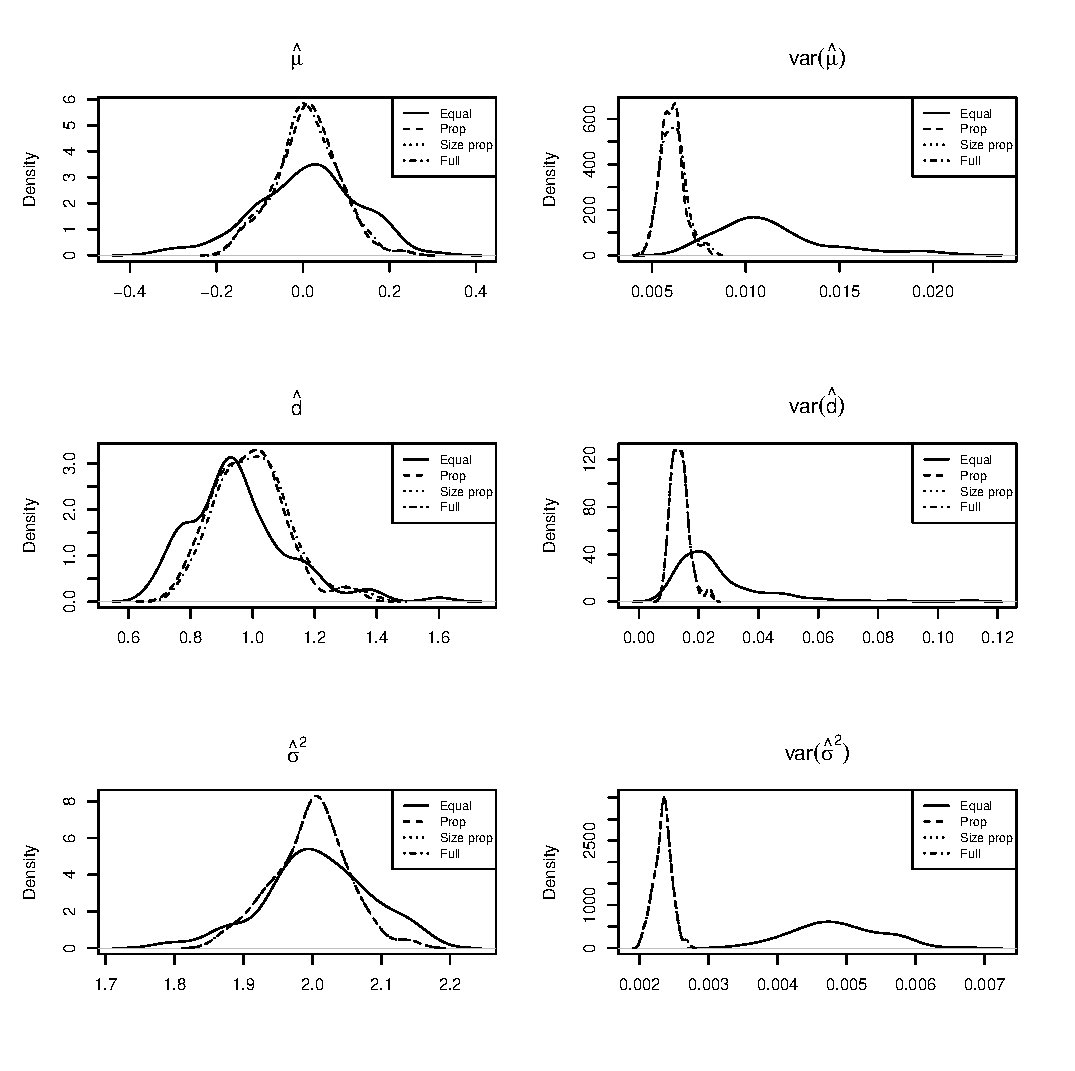
\includegraphics[width=\textwidth]{aCS_diff_comb2.eps}
\caption{\small \linespread{1.1} First simulation study. Setting 3. Combining the results from the four splits, using equal, proportional, and size proportional weights. This is compared with full maximum likelihood.} \label{CS_diff_comb2}
\end{figure}


\subsection{Optimal, Approximate Optimal, and Iterated Optimal Weights}

Optimal weights were discussed in Section~6.1.1.
%\ref{owcs}. 
When we plug the MLE's into the optimal weights, the result of using these weights is the MLE's itself. Of course, this is a circular reasoning, which is why one needs to resort to, for example, the approximate or iterated optimal weights derived in Section~6.1.2.
%\ref{iaow}. 
For both of these, using Settings~1--3, we conducted simulations. They are reported in Figures~\ref{Setting1_opt}--\ref{Setting3_opt}.
\begin{figure}[!t]
\centering
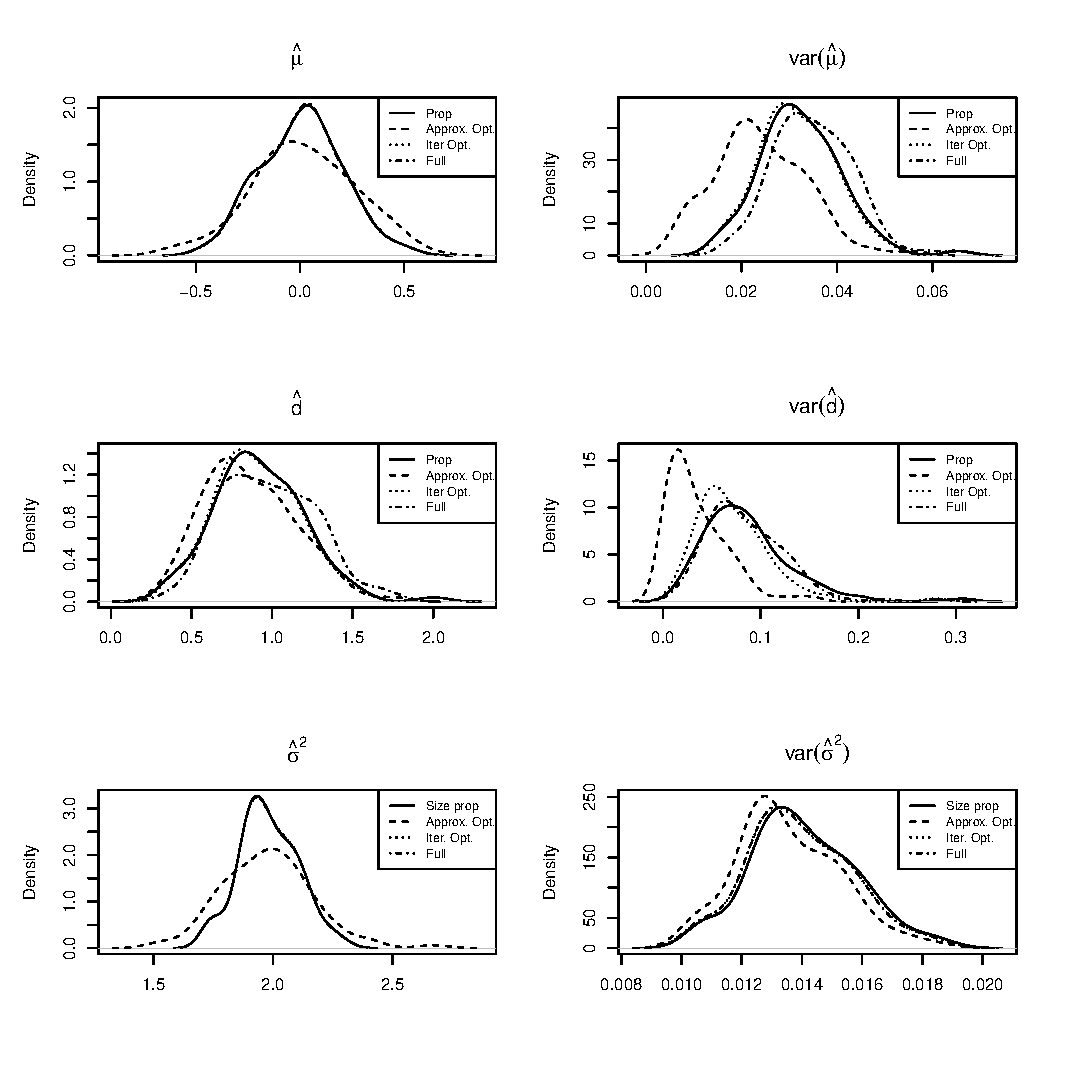
\includegraphics[width=\textwidth]{aSetting1_opt.eps}
\caption{\small \linespread{1.1} First simulation study. Setting 1. (Size) proportional, approximate, and iterated optimal weights, as well as full maximum likelihood.} \label{Setting1_opt}
\end{figure}
\begin{figure}[!t]
\centering
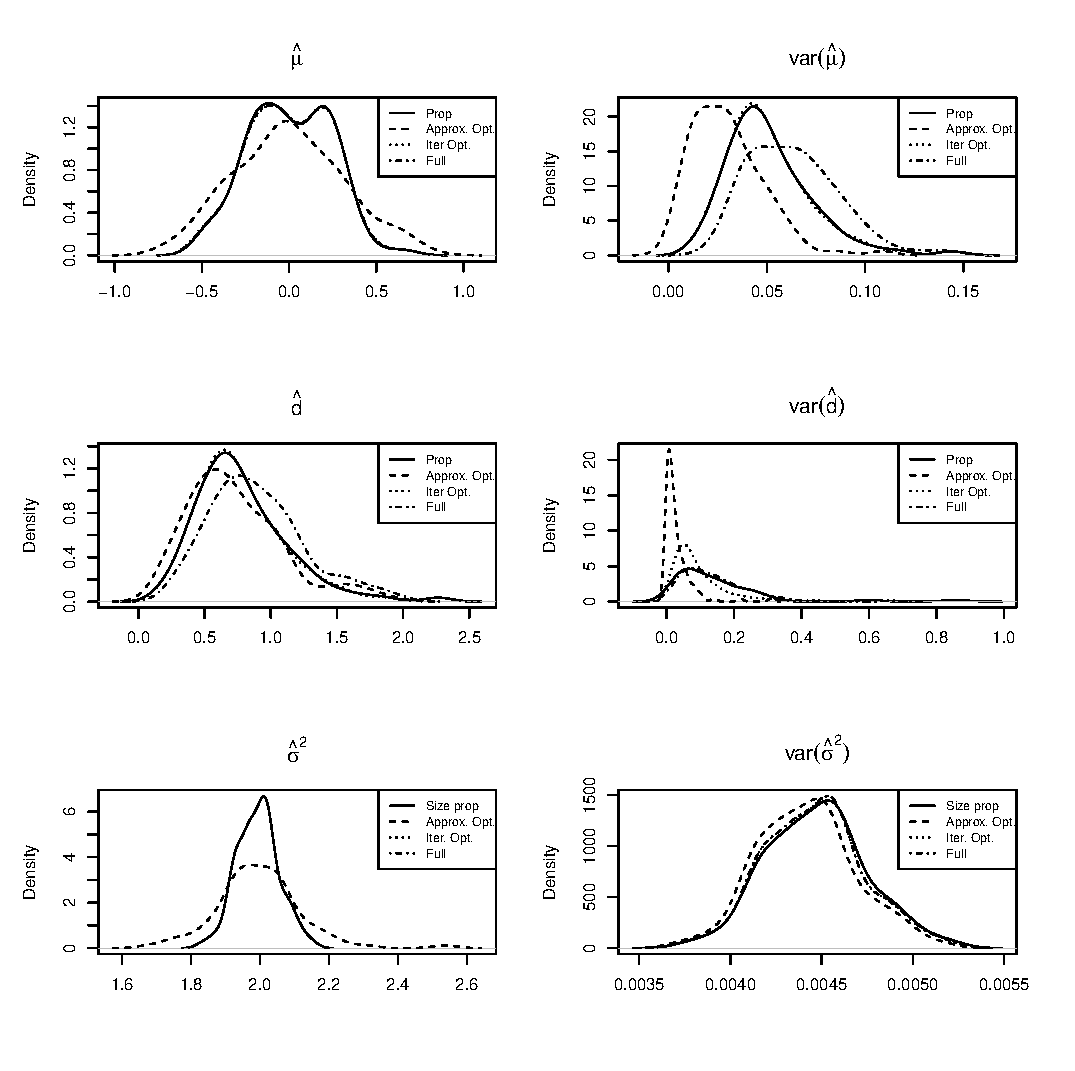
\includegraphics[width=\textwidth]{aSetting2_opt.eps}
\caption{\small \linespread{1.1} First simulation study. Setting 2. (Size) proportional, approximate, and iterated optimal weights, as well as full maximum likelihood.} \label{Setting2_opt}
\end{figure}
\begin{figure}[!t]
\centering
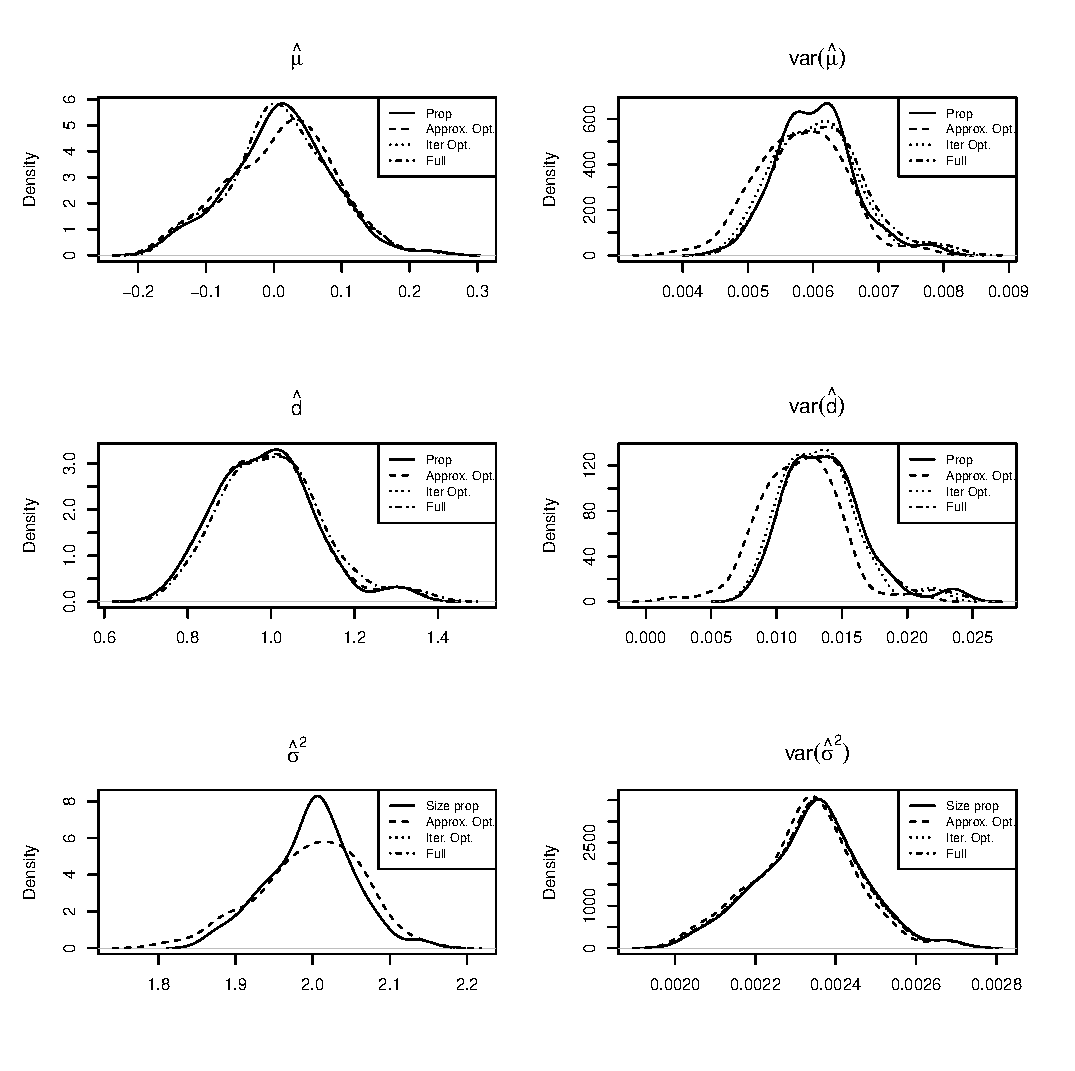
\includegraphics[width=\textwidth]{aSetting3_opt.eps}
\caption{\small \linespread{1.1} First simulation study. Setting 3. (Size) proportional, approximate, and iterated optimal weights, as well as full maximum likelihood.} \label{Setting3_opt}
\end{figure}

It is noteworthy that the behavior of the iterated optimal weights depends on $c_k$ and $n_k$. First, they often but not always converge in a single iteration; the maximum number of iterations observed in our simulations being~6. Second, the iterated optimal weights  converge to size optimal weights for $\sigma^2$ and to proportional weights for $d$.

Taken together, it follows that both approximately optimal and iterated optimal weights provide excellent results. The specific attraction of the approximate optimal weights is that they obviate the need for iteration, which is a factor of stability and speed.


\section{Details About the Second Simulation Study}
\label{simapptwee}

The aim of this study is to compare the proposed method to two alternatives: 
\begin{enumerate}
\item full maximum likelihood;
\item the proposed  sample-splitting method, allowing for closed forms;
\item using multiple imputation (MI) first, to render the clusters of equal sizes, and then apply closed-form solutions to the augmented balanced data, together with the combination rules.
\end{enumerate}

\subsection{Simulation Plan}

In order to study the effect of cluster sizes ($n_k$) and number of clusters of each size ($c_k$), 5 different configurations are considered:
\begin{description}
\item[Config.~1.] $c_k=(15,25,30,20,10)$, $n_k=(8,5,3,9,15)$;
\item[Config.~2.] $c_k=(150,250,300,200,100)$, $n_k=(8,5,3,9,15)$;
\item[Config.~3.] $c_k=(1500,2500,3000,2000,1000)$, $n_k=(8,5,3,9,15)$;
\item[Config.~4.] $c_k=(15,25,30,20,10)$, $n_k=(80,50,30,90,150)$;
\item[Config.~5.] $c_k=(15,25,30,20,10)$, $n_k=(800,500,300,900,1500)$.
\end{description}
 Each configuration is repeated $100$ times.

Each cluster is generated from a CS model with $\mu_0=0$, $d_0=1$, and $\sigma^2_0=4$. 

For estimating the parameters using the full unbalanced data, PROC MIXED in SAS (Version 9.4) is used with the covariance structure in the REPEATED statement set to {\tt{type=cs}}.


The closed form solutions and their variances are implemented in {\tt R} in three different ways. First, the formulas  are implemented directly using `for' loops. Following the ideas in \cite{sikorska2013_2}, it might be faster to replace `for' loops with vectorized computation. For $\widehat{\mu}_k$ it is straightforward, since one just needs to compute an arithmetic average. If $Z$ is a $n_k$ times $c_k$ matrix with its $i$th column defined as $Z_i^{(k)}=\left(Y_i^{(k)} - \mu_k \mathbf{1}_{n_k} \right)$, then computing $\sum_{i=1}^ {c_k}  Z_i^{(k)'} Z_i^{(k)}$  is equivalent to replacing each element in matrix $Z$ by its square, and then sum over the sum of its columns. Furthermore, $J_{n_k} Z_i^{(k)}$ would simply compute the sum of columns in matrix $Z$. Therefore, $\sum_{i=1}^{c_k} Z_i^{(k)'} J_{n_k} Z_I^{(k)}$ is equivalent to post-multiplying $Z$ by the sum of its columns and then sum over this vector. In this way, within each split, the parameters can be estimated avoiding `for' loops. 

Second, it is also possible to find the estimates for all of the splits at once instead of computing them separately. 

A third way consists of calculating all the estimates together and not split by split in a `for' loop. This approach is possible via imposing balance through adding missing values in the matrix but, when multiplying and summing, ignoring the missing values. This is very easy in {\tt R}. 

We will compare computation time between these three approaches, for the five configurations.

Additionally, to combine the results from sample splitting, the same
weights as used in the case study are considered here as well: equal, proportional, approximate scalar, scalar, and approximate optimal. In the case of the approximate optimal weights both simple and proper variances are calculated. 

For the multiple imputation based approach, $M=20$ imputations are considered and the conventional combination rules applied.

 Note that the MI approach cannot be used with configurations 1, 4, and 5, because the number of available subjects in the observed dataset is less than the number of repeated measurements, leading to a singular covariance matrix. From the remaining configurations 2 and 3, we have chosen \#2, which implies smaller numbers and hence is more challenging.

For each configuration we report three results: the estimated parameters, their standard errors, and the mean square error (MSE). Furthermore, we report computation time. 

\subsection{Simulation results}

\begin{table}[ht]
\centering
\caption{\small \linespread{1.1} Second simulation study. Mean, standard deviation (S.D.) and MSE for $\mu$ among 100 replications for each configuration using different combination weights comparing with full sample MLE.}
\label{tab_mu_est}

\vspace*{2mm}


\resizebox{\textwidth}{!}{%
\def\arraystretch{0.6} \begin{tabular}{cccccccc}
  \hline\hline
Config.& & Equal & Prop & Approx.~sc. & Scalar & Approx.~opt. & ML \\ 
  \hline
 & Mean & -1.72277E-02 & -1.51605E-02 & -1.51605E-02 & -1.21296E-02 & -1.21296E-02 & -1.56028E-02 \\ 
1 & S.D. & (1.32751E-01) & (1.28989E-01) & (1.28989E-01) & (1.32435E-01) & (1.32435E-01) & (1.29150E-01) \\ 
 & MSE & 1.77434E-02 & 1.67015E-02 & 1.67015E-02 & 1.75108E-02 & 1.75108E-02 & 1.67564E-02 \\ 
 & Mean & -9.39926E-04 & 6.93419E-04 & 6.93419E-04 & 1.27613E-03 & 1.27613E-03 & 7.59533E-04 \\ 
2 & S.D. & (3.93526E-02) & (3.95534E-02) & (3.95534E-02) & (3.84321E-02) & (3.84321E-02) & (3.83996E-02) \\ 
 & MSE & 1.53403E-03 & 1.54930E-03 & 1.54930E-03 & 1.46389E-03 & 1.46389E-03 & 1.46036E-03 \\ 
 & Mean & -8.30934E-04 & -1.25609E-03 & -1.25609E-03 & -1.26810E-03 & -1.26810E-03 & -1.31356E-03 \\ 
3 & S.D.& (1.44839E-02) & (1.47545E-02) & (1.47545E-02) & (1.41310E-02) & (1.41310E-02) & (1.41704E-02) \\ 
 & MSE & 2.08376E-04 & 2.17095E-04 & 2.17095E-04 & 1.99298E-04 & 1.99298E-04 & 2.00517E-04 \\ 
 & Mean & 9.30928E-03 & 2.53713E-03 & 2.53713E-03 & 8.29367E-03 & 8.29367E-03 & 2.82086E-03 \\ 
4 & S.D. & (9.26881E-02) & (8.32009E-02) & (8.32009E-02) & (9.76672E-02) & (9.76672E-02) & (8.28999E-02) \\ 
 & MSE & 8.59183E-03 & 6.85960E-03 & 6.85960E-03 & 9.51227E-03 & 9.51227E-03 & 6.81163E-03 \\ 
 & Mean & 9.77532E-03 & 1.02173E-02 & 1.02173E-02 & 8.72381E-03 & 8.72381E-03 & 1.02422E-02 \\ 
5 & S.D. & (1.09769E-01) & (1.04876E-01) & (1.04876E-01) & (1.04982E-01) & (1.04982E-01) & (1.04847E-01) \\ 
 & MSE & 1.20243E-02 & 1.09934E-02 & 1.09934E-02 & 1.09872E-02 & 1.09872E-02 & 1.09880E-02 \\ 
   \hline\hline
\end{tabular}}
\end{table}



\begin{table}[ht]
\centering
\caption{\small \linespread{1.1} Second simulation study. Mean and standard deviation (S.D.) for standard errors of $\mu$ estimates in 100 replications for each configuration using different combination weights comparing with full sample MLE.}
\label{tab_mu_std}

\vspace*{2mm}

\resizebox{\textwidth}{!}{%
\def\arraystretch{0.6} \begin{tabular}{ccccccccc}
  \hline\hline
Config.& & Equal & Prop & Approx.~sc. & Scalar & Simple opt. & Proper opt. & ML \\ 
  \hline
1  &Mean & 1.29844E-01 & 1.29733E-01 & 1.29733E-01 & 1.20593E-01 & 1.20593E-01 & 1.41085E-01 & 1.29648E-01 \\ 
  &S.D.& (1.18175E-02) & (1.07496E-02) & (1.07496E-02) & (1.09122E-02) & (1.09122E-02) & (2.25155E-02) & (9.95614E-03) \\ 
2  &Mean & 4.23655E-02 & 4.23056E-02 & 4.23056E-02 & 4.11657E-02 & 4.11657E-02 & 4.12635E-02 & 4.14298E-02 \\ 
  &S.D.& (1.08386E-03) & (8.88747E-04) & (8.88747E-04) & (8.71465E-04) & (8.71465E-04) & (8.90259E-04) & (8.66432E-04) \\ 
3  &Mean & 1.34008E-02 & 1.33822E-02 & 1.33822E-02 & 1.30725E-02 & 1.30725E-02 & 1.30728E-02 & 1.30799E-02 \\ 
  &S.D.& (1.21880E-04) & (9.92324E-05) & (9.92324E-05) & (9.68871E-05) & (9.68871E-05) & (9.68974E-05) & (9.62652E-05) \\ 
4  &Mean & 1.06373E-01 & 1.01232E-01 & 1.01232E-01 & 9.60807E-02 & 9.60807E-02 & 3.30358E-01 & 1.03382E-01 \\ 
  &S.D.& (9.80278E-03) & (7.26031E-03) & (7.26031E-03) & (8.36242E-03) & (8.36242E-03) & (1.39042E-01) & (7.17708E-03) \\ 
4  &Mean & 1.05176E-01 & 9.84615E-02 & 9.84615E-02 & 9.45066E-02 & 9.45066E-02 & 2.81427E+00 & 1.00533E-01 \\ 
  &S.D.& (1.10711E-02) & (8.18259E-03) & (8.18259E-03) & (8.14229E-03) & (8.14229E-03) & (1.41211E+00) & (8.28537E-03) \\ 
\hline\hline  
\end{tabular}}
\end{table}




















\begin{figure}
\centering


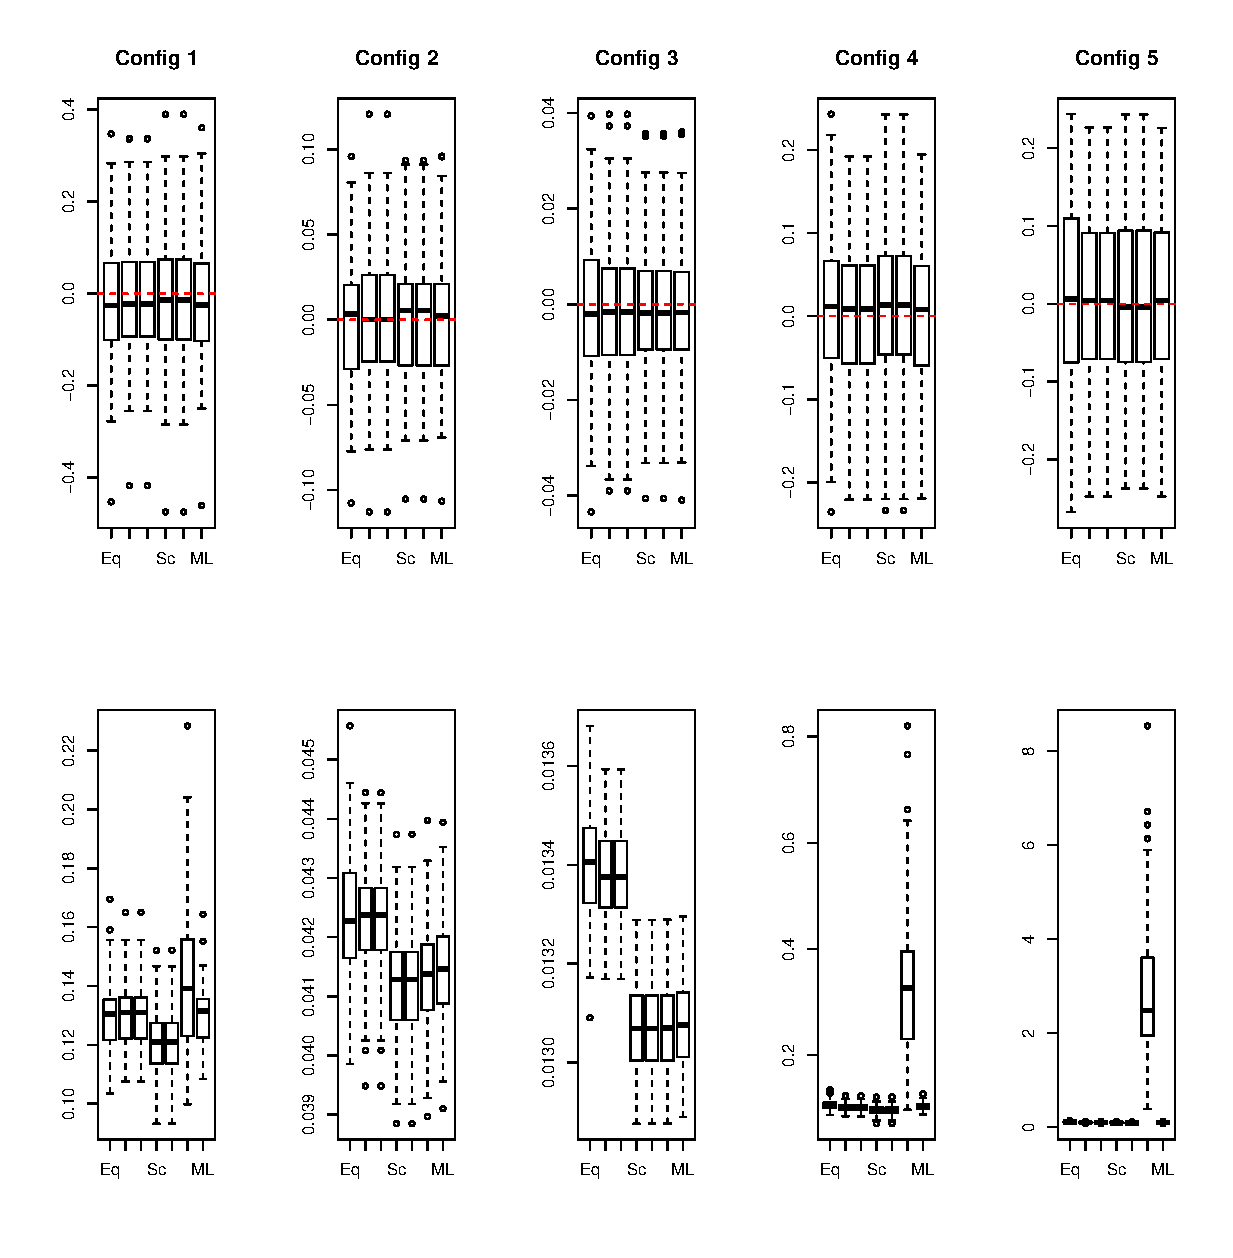
\includegraphics[width=\textwidth]{fig_mu.eps}
\caption{\small \linespread{1.1}  Second simulation study. Estimates for $\mu$ (first row) and its standard error (second row).} \label{fig_mu}
\end{figure}




\begin{table}[ht]
\centering
\caption{\small \linespread{1.1} Second simulation study. Mean, standard deviation (S.D.) and MSE for $d$ estimates in 100 replications for each configuration using different combination weights comparing with full sample MLE.}
\label{tab_d_est}

\vspace*{2mm}

\resizebox{\textwidth}{!}{%
\def\arraystretch{0.6} \begin{tabular}{cccccccc}
  \hline\hline
Config.& & Equal & Prop & Approx.~sc. & Scalar & Approx.~opt & ML \\ 
  \hline
 & Mean & 9.09580E-01 & 9.00788E-01 & 9.00788E-01 & 6.63293E-01 & 6.71111E-01 & 9.86549E-01 \\ 
1 & S.D. & (2.66885E-01) & (2.99736E-01) & (2.99736E-01) & (2.70556E-01) & (2.79060E-01) & (2.55874E-01) \\ 
 & MSE & 7.86910E-02 & 9.87862E-02 & 9.87862E-02 & 1.85840E-01 & 1.85264E-01 & 6.49975E-02 \\ 
 & Mean & 9.98984E-01 & 9.97534E-01 & 9.97534E-01 & 9.72269E-01 & 9.73771E-01 & 1.00712E+00 \\ 
2 & S.D. & (7.44958E-02) & (8.28143E-02) & (8.28143E-02) & (7.28186E-02) & (7.22762E-02) & (7.08463E-02) \\ 
 & MSE & 5.49515E-03 & 6.79570E-03 & 6.79570E-03 & 6.01854E-03 & 5.85958E-03 & 5.01969E-03 \\ 
 & Mean & 1.00004E+00 & 9.99697E-01 & 9.99697E-01 & 9.97218E-01 & 9.97153E-01 & 1.00019E+00 \\ 
3 & S.D. & (2.61046E-02) & (2.82480E-02) & (2.82480E-02) & (2.48989E-02) & (2.48068E-02) & (2.44715E-02) \\ 
 & MSE & 6.74637E-04 & 7.90063E-04 & 7.90063E-04 & 6.21496E-04 & 6.17332E-04 & 5.92900E-04 \\ 
 & Mean & 9.40257E-01 & 9.50756E-01 & 9.50756E-01 & 7.65219E-01 & 7.65362E-01 & 9.96005E-01 \\ 
4 & S.D. & (1.53414E-01) & (1.48216E-01) & (1.48216E-01) & (1.91865E-01) & (1.91614E-01) & (1.49451E-01) \\ 
 & MSE & 2.68697E-02 & 2.41734E-02 & 2.41734E-02 & 9.15661E-02 & 9.14038E-02 & 2.21282E-02 \\ 
 & Mean & 9.63459E-01 & 9.68182E-01 & 9.68182E-01 & 8.21266E-01 & 8.21270E-01 & 1.00958E+00 \\ 
5 & S.D. & (1.73767E-01) & (1.63471E-01) & (1.63471E-01) & (1.72162E-01) & (1.72163E-01) & (1.69235E-01) \\ 
 & MSE & 3.12283E-02 & 2.74677E-02 & 2.74677E-02 & 6.12894E-02 & 6.12881E-02 & 2.84459E-02 \\ 
\hline
   \hline
\end{tabular}}
\end{table}



\begin{table}[ht]
\centering
\caption{\small \linespread{1.1}Second simulation study. Mean and standard deviation (S.D.) for standard errors of $d$ estimates in 100 replications for each configuration using different combination weights comparing with full sample MLE.}
\label{tab_d_std}

\vspace*{2mm}

\resizebox{\textwidth}{!}{%
\def\arraystretch{0.6} \begin{tabular}{ccccccccc}
  \hline\hline
Config.& & Equal & Prop. & Approx.~sc. & Scalar & Simple opt. & Proper opt. & ML \\ 
  \hline
1 & Mean & 5.30888E-01 & 6.76159E-01 & 6.76159E-01 & 4.83519E-01 & 1.95328E-01 & 4.66561E+00 & 2.36408E-01 \\ 
 & S.D. & (1.00495E-01) & (1.66365E-01) & (1.66365E-01) & (1.10589E-01) & (4.01066E-02) & (1.40173E+00) & (3.91752E-02) \\ 
2 & Mean & 1.60365E-01 & 2.03126E-01 & 2.03126E-01 & 1.45284E-01 & 7.48056E-02 & 1.47955E+00 & 7.60798E-02 \\ 
 & S.D. & (8.29444E-03) & (1.42616E-02) & (1.42616E-02) & (8.70034E-03) & (3.35411E-03) & (1.31587E-01) & (3.26483E-03) \\ 
3 & Mean & 5.02596E-02 & 6.34861E-02 & 6.34861E-02 & 4.56061E-02 & 2.39463E-02 & 4.67989E-01 & 2.39748E-02 \\ 
 & S.D. & (8.43976E-04) & (1.44201E-03) & (1.44201E-03) & (8.34510E-04) & (3.68251E-04) & (1.24414E-02) & (3.66865E-04) \\ 
4 & Mean & 1.62410E-01 & 1.59656E-01 & 1.59656E-01 & 1.34256E-01 & 1.24552E-01 & 2.35351E-01 & 1.51740E-01 \\ 
 & S.D. & (2.83009E-02) & (2.05482E-02) & (2.05482E-02) & (2.31559E-02) &(2.51091E-02) & (3.00109E-02) & (2.11541E-02) \\ 
5 & Mean & 1.54122E-01 & 1.43313E-01 & 1.43313E-01 & 1.22117E-01 & 1.22024E-01 & 1.70868E-01 & 1.43764E-01 \\ 
 & S.D. & (3.48725E-02) & (2.50371E-02) & (2.50371E-02) & (2.30972E-02)& (2.31064E-02) & (3.70951E-02) & (2.38992E-02) \\ 
   \hline\hline
\end{tabular}}
\end{table}


\begin{figure}
\centering
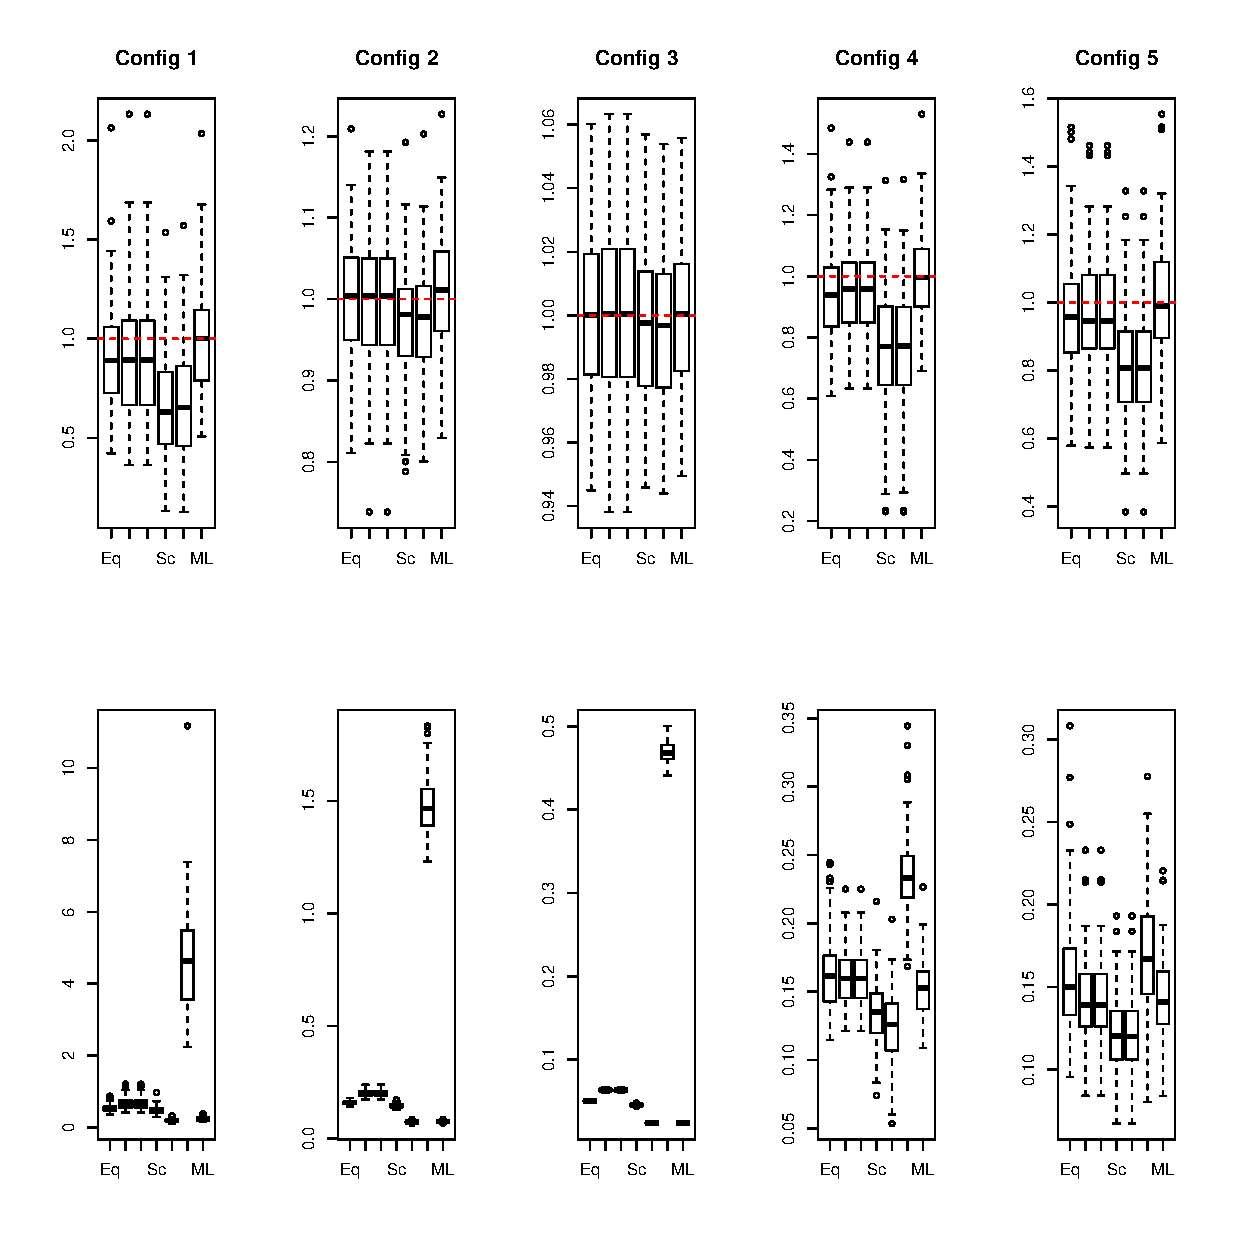
\includegraphics[width=\textwidth]{fig_d.eps}
\caption{\small \linespread{1.1} Second simulation study. Estimates for $d$ (first row) and standard errors ( second row).} \label{fig_d}
\end{figure}






\begin{table}[ht]
\centering
\caption{\small \linespread{1.1}Second simulation study. Mean, standard deviation (S.D.) and MSE for $\sigma^2$ estimates in 100 replications for each configuration using different combination weights comparing with full sample MLE.}
\label{tab_sigma2_est}

\vspace*{2mm}

\resizebox{\textwidth}{!}{%
\def\arraystretch{0.6} \begin{tabular}{cccccccc}
  \hline\hline
Config.& & Equal & Prop. & Approx.~sc. & Scalar & Approx.~opt. & ML \\ 
  \hline
 & Mean & 3.98608E+00 & 3.99739E+00 & 3.98571E+00 & 3.98364E+00 & 3.87487E+00 & 3.98075E+00 \\ 
1 & S.D. & (2.50882E-01) & (2.95821E-01) & (2.35138E-01) & (2.33650E-01) & (2.38167E-01) & (2.30477E-01) \\ 
 & MSE & 6.25062E-02 & 8.66420E-02 & 5.49414E-02 & 5.43140E-02 & 7.18141E-02 & 5.29588E-02 \\ 
 & Mean & 4.00184E+00 & 4.00681E+00 & 4.00177E+00 & 4.00087E+00 & 3.99027E+00 & 4.00064E+00 \\ 
2 & S.D. & (7.85190E-02) & (9.05849E-02) & (7.57443E-02) & (7.56486E-02) & (7.50477E-02) & (7.51739E-02) \\ 
 & MSE & 6.10698E-03 & 8.16998E-03 & 5.68296E-03 & 5.66624E-03 & 5.67055E-03 & 5.59502E-03 \\ 
 & Mean & 4.00509E+00 & 4.00491E+00 & 4.00575E+00 & 4.00590E+00 & 4.00472E+00 & 4.00587E+00 \\ 
3 & S.D. & (2.45760E-02) & (2.82395E-02) & (2.36027E-02) & (2.36983E-02) & (2.37694E-02) & (2.36697E-02) \\ 
 & MSE & 6.23828E-04 & 8.13646E-04 & 5.84605E-04 & 5.90806E-04 & 5.81652E-04 & 5.89081E-04 \\ 
 & Mean & 4.01402E+00 & 4.01190E+00 & 4.01302E+00 & 4.01304E+00 & 4.00363E+00 & 4.01306E+00 \\ 
4 & S.D. & (7.69655E-02) & (8.78962E-02) & (7.32088E-02) & (7.31202E-02) & (7.20589E-02) & (7.31207E-02) \\ 
 & MSE & 6.06101E-03 & 7.79021E-03 & 5.47558E-03 & 5.46319E-03 & 5.15372E-03 & 5.46370E-03 \\ 
 & Mean & 4.00346E+00 & 4.00338E+00 & 4.00292E+00 & 4.00292E+00 & 4.00192E+00 & 4.00292E+00 \\ 
5 & S.D. & (2.56561E-02) & (2.79741E-02) & (2.46670E-02) & (2.46664E-02) & (2.46901E-02) & (2.46669E-02) \\ 
 & MSE & 6.63599E-04 & 7.86128E-04 & 6.10884E-04 & 6.10854E-04 & 6.07187E-04 & 6.10909E-04 \\ 
   \hline\hline
\end{tabular}}
\end{table}




\begin{table}[ht]
\centering
\caption{\small \linespread{1.1} Second simulation study. Mean and standard deviation (S.D.) for standard errors of $\sigma^2$ estimates in 100 replications for each configuration using different combination weights comparing with full sample MLE.}
\label{tab_sigma2_std}

\vspace*{2mm}

\resizebox{\textwidth}{!}{%
\def\arraystretch{0.6} \begin{tabular}{ccccccccc}
  \hline\hline
Config.& & Equal & Prop. & Approx.~sc. & Scalar & Simple opt. & Proper opt. & ML \\ 
  \hline
1  &Mean & 2.53758E-01 & 2.95524E-01 & 2.40482E-01 & 2.38699E-01 & 2.30855E-01 & 2.88730E+01 & 2.35804E-01 \\ 
  &S.D. & (1.98892E-02) & (3.33124E-02) & (1.45355E-02) & (1.39849E-02) & (1.38813E-02) & (6.93951E+00) & (1.34905E-02) \\ 
2  &Mean  & 7.98210E-02 & 9.26570E-02 & 7.57927E-02 & 7.53242E-02 & 7.48395E-02 & 8.82494E+00 & 7.49872E-02 \\ 
  &S.D. & (1.84469E-03) & (3.08841E-03) & (1.45443E-03) & (1.42354E-03) & (1.40575E-03) & (6.92140E-01) & (1.39989E-03) \\ 
3  &Mean  & 2.52202E-02 & 2.92034E-02 & 2.39687E-02 & 2.38353E-02 & 2.37400E-02 & 2.78559E+00 & 2.37444E-02 \\ 
  &S.D. & (1.85701E-04) & (3.12856E-04) & (1.42587E-04) & (1.40888E-04) & (1.40071E-04) & (6.70930E-02) & (1.39784E-04) \\ 
4  &Mean  & 7.22378E-02 & 8.07793E-02 & 7.01684E-02 & 7.01663E-02 & 6.99970E-02 & 7.23107E+00 & 7.01238E-02 \\ 
  &S.D. & (1.54384E-03) & (2.35043E-03) & (1.28712E-03) & (1.28385E-03) & (1.26263E-03) & (5.28710E-01) & (1.27765E-03) \\ 
5  &Mean  & 2.25782E-02 & 2.52054E-02 & 2.19702E-02 & 2.19702E-02 & 2.19647E-02 & 2.23651E+00 & 2.19689E-02 \\ 
  &S.D. & (1.55999E-04) & (2.29649E-04) & (1.35364E-04) & (1.35358E-04) & (1.35462E-04) & (5.50362E-02) & (1.35379E-04) \\ 
   \hline\hline
\end{tabular}}
\end{table}



\begin{figure}
\centering
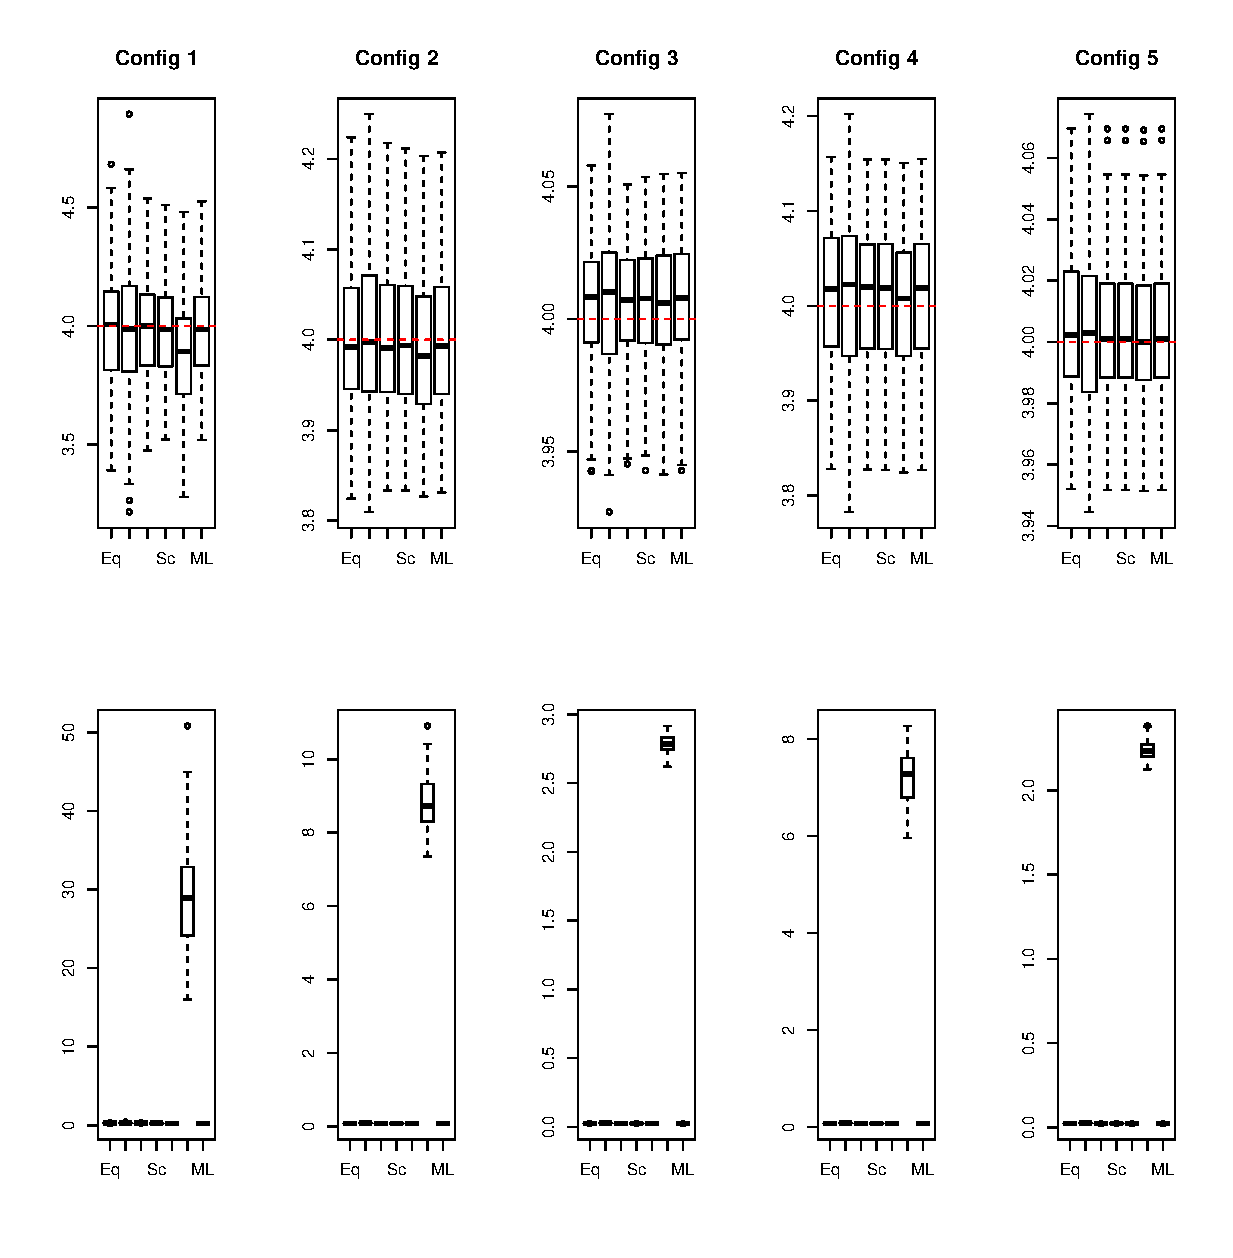
\includegraphics[width=\textwidth]{fig_sigma2.eps}
\caption{\small \linespread{1.1}  Second simulation study. Estimates for $\sigma^2$ (first row) and standard errors (second row).} \label{fig_sigma2}
\end{figure}

\begin{table}[ht]
\centering
\caption{\small \linespread{1.1} Second simulation study. Computation time (in seconds) using closed-form solutions with different implementation forms, compared to PROC MIXED.}

\vspace*{2mm}

\def\arraystretch{0.6} \begin{tabular}{cccccc}
  \hline\hline
&&\multicolumn{2}{c}{Split by split} & & PROC \\ 
\cline{3-4}
Config.& & without loops &  using loops & Together & MIXED \\ 
  \hline
1& Mean & \textbf{0.00520} & 0.00980 & 0.00640 & 0.34155 \\ 
 & S.D. & (0.00882) & (0.00943) & (0.00823) & (0.17711) \\ 
2  &Mean & \textbf{0.02150} & 0.07340 & 0.05660 & 0.35575 \\ 
  &S.D. & (0.01617) & (0.02006) & (0.09662) & (0.03073) \\ 
3  &Mean & \textbf{0.17980} & 0.73480 & 0.43400 & 0.81783 \\ 
  &S.D. & (0.02292) & (0.05835) & (0.11543) & (0.02582) \\ 
4  &Mean & \textbf{0.00220} & 0.00610 & 0.00360 & 2.58808 \\ 
  &S.D. & (0.00579) & (0.01497) & (0.00689) & (0.40720) \\ 
5  &Mean & 0.04030 & 0.27490 &\textbf{ 0.02130} & 629.58333 \\ 
  &S.D. & (0.01521) & (0.01941) & (0.00872) & (116.09435) \\ 
\hline\hline
\end{tabular}
\end{table}



\begin{table}[ht]
\centering
\caption{\small \linespread{1.1} Second simulation study. Mean, standard deviation (S.D.) and MSE for CS parameter estimates in 100 replications for configuration 2 using different combination weights comparing with full sample MLE and MI-MLE.}
\label{tab_mi_est}

\vspace*{2mm}

\resizebox{\textwidth}{!}{%
\def\arraystretch{0.6} \begin{tabular}{rcccccccc} 
  \hline\hline
& & Equal & Prop. & Approx.~sc.\ & Scalar & Approx.~opt. & MI & ML \\ 
  \hline
&Mean & -5.09643E-03 & -2.62061E-03 & -2.62061E-03 & -2.88933E-03 & -2.88933E-03 & -8.04195E-03 & -3.28224E-03 \\ 
$\mu$&  S.D. & (4.85424E-02) & (4.91772E-02) & (4.91772E-02) & (4.68032E-02) & (4.68032E-02) & (6.00662E-02) & (4.71723E-02) \\ 
&  MSE & 2.35877E-03 & 2.40108E-03 & 2.40108E-03 & 2.17698E-03 & 2.17698E-03 & 3.63654E-03 & 2.21375E-03 \\ 
&  Mean & 9.98392E-01 & 9.95216E-01 & 9.95216E-01 & 9.70589E-01 & 9.71627E-01 & 3.51123E-02 & 9.92960E-01 \\ 
$d$&   S.D. & (7.33193E-02 & (7.46946E-02) & (7.46946E-02) & (7.59516E-02) & (7.53362E-02) & (1.83983E-02) & (7.50610E-02) \\ 
&   MSE & 5.32455E-03 & 5.54638E-03 & 5.54638E-03 & 6.57598E-03 & 6.42380E-03 & 9.31343E-01 & 5.62737E-03 \\ 
& Mean & 4.00782E+00 & 4.00791E+00 & 4.00581E+00 & 4.00544E+00 & 3.99400E+00 & 5.32627E+00 & 4.00347E+00 \\ 
$\sigma^2$&   S.D. & (7.66500E-02) & (8.98881E-02) & (7.19708E-02) & (7.13441E-02) & (7.19080E-02) & (1.55770E-01) & (7.56968E-02) \\ 
&  MSE & 5.87763E-03 & 8.06169E-03 & 5.16181E-03 & 5.06871E-03 & 5.15505E-03 & 1.78301E+00 & 5.68472E-03 \\ 
   \hline\hline
\end{tabular}}
\end{table}



\begin{table}[ht]
\caption{\small \linespread{1.1} Second simulation study. Mean and standard deviation (S.D.) for the standard error of CS parameter estimates in 100 replications for configuration 2 using different combination weights comparing with full sample MLE and MI-MLE.}
\label{tab_mi_std}

\vspace*{2mm}

\centering
\resizebox{\textwidth}{!}{%
\def\arraystretch{0.6} \begin{tabular}{rccccccccc}
  \hline\hline
 & & Equal & Prop. & Approx.~sc. & Scalar & Simple opt. & Proper opt. & MI &ML \\   
  \hline
$\mu$ &Mean & 4.24162E-02 & 4.22766E-02 & 4.22766E-02 & 4.11356E-02 & 4.11356E-02 & 4.12439E-02 & 4.95431E-02 & 4.14004E-02 \\ 
 & S.D. & (1.21548E-03) & (8.59430E-04) & (8.59430E-04) & (9.31222E-04) & (9.31222E-04) & (9.42598E-04) & (7.65032E-03) & (9.11785E-04) \\ 
$d$ & Mean & 1.60545E-01 & 2.02922E-01 & 2.02922E-01 & 1.45623E-01 & 7.47531E-02 & 1.48865E+00 & 9.10211E-02 & 7.54391E-02 \\ 
 &  S.D. & (8.88524E-03) & (1.47416E-02) & (1.47416E-02) & (9.84170E-03) & (3.76197E-03) & (1.29914E-01) & (5.18621E-03) & (3.38044E-03) \\ 
$\sigma^2$ & Mean & 7.99442E-02 & 9.26315E-02 & 7.58626E-02 & 7.54139E-02 & 7.49171E-02 & 8.86450E+00 & 1.64310E-01 & 7.50377E-02 \\ 
 &  S.D. & (1.87358E-03) & (3.14842E-03) & (1.39531E-03) & (1.34244E-03) & (1.33807E-03) & (6.56714E-01) & (2.27104E-02) & (1.42688E-03) \\ 
   \hline\hline
\end{tabular}}
\end{table}



\begin{figure}[t]
\centering
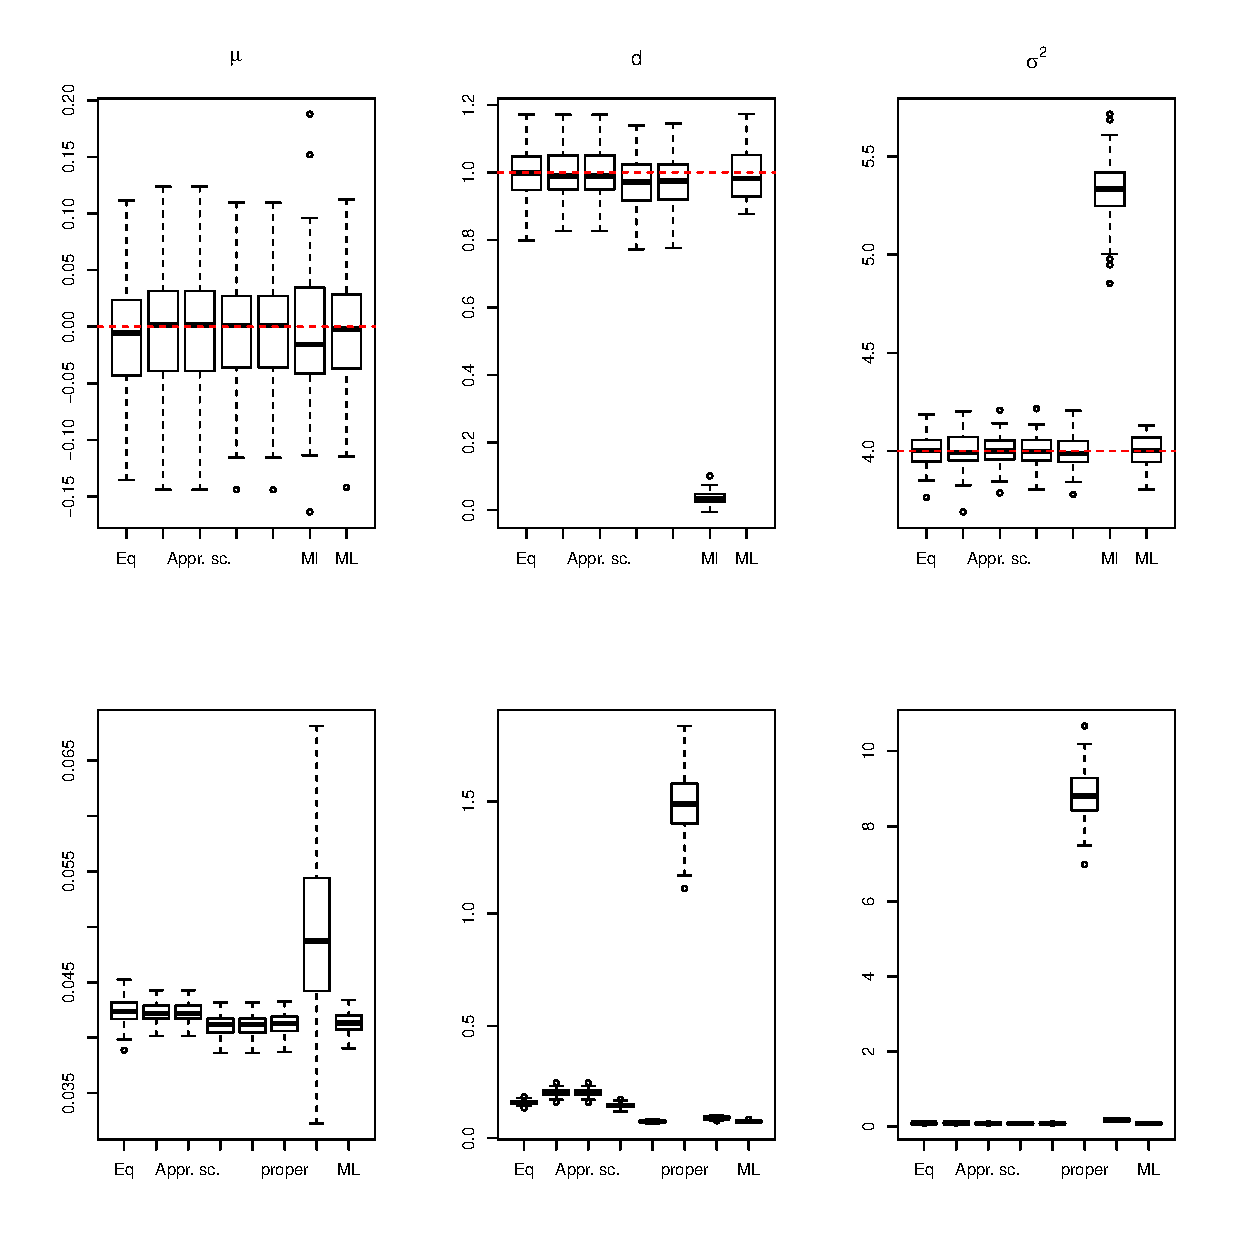
\includegraphics[width=0.9\textwidth]{fig_mi.eps}
\caption{\small \linespread{1.1}  Second simulation study. Estimated CS parameters (first row) and their standard error (second row) using sample splitting, MI-MLE, and MLE.} \label{fig_mi}
\end{figure}

Based on the simulation results, it appears that  using equal weights is not recommended, while using proportional weights produces results comparable with ML. Of course, in case of $\sigma^2$ the approximate scalar weights  work better comparing with ML. An interesting outcome of the simulation is that by keeping the number of clusters of different sizes constant, but allowing the cluster sizes to increase, improves estimation of  $\sigma^2$, while increasing the number of clusters and keeping their sizes constant improves the estimation of  $d$. This is not surprising, because $d$ is the between-cluster variability, which is easier to estimate from a larger number of clusters. This should be seen against the background of relatively small differences anyway. 

The results based on MI are not comparable with sample-splitting results. In particular, the variance component $d$ is underestimated using MI, while $\sigma^2$ is overestimated.  The larger standard errors in this case suggest that the sample-splitting methods use information more efficiently. 

Comparing computation times, the closed-form approaches are the clear winners, further enhanced by smaller standard errors.  Furthermore, it follows that computing the estimates in a semi-parallel fashion, thus avoiding `for' loops within the splits but using then  between splits, is most efficient. Unless the $n_k$'s are very large, computing all  estimates at once is the most efficient. Of course, if the estimates for different splits can be done in parallel (without `for' loops), this is more efficient than estimating them all at once.



%% Ar1
\section{The Balanced Conditionally Independent Model\label{bcim}}

In this case, one imposes the following structure on (\ref{lmmhier}):
\begin{itemize}
\item \Xik\ can be rewritten in terms of a first matrix that imposes structure between clusters (e.g., treatment effect), termed \Aik, and a second one that imposes structure within clusters (e.g., time evolution), $\Tik'=(\Zik',\Qik')'$.
\item The matrices \Aik, \Zik, and \Qik\ are constant among all clusters of size~$n_k$.
\item The matrix $\Sigma_i^{(k)}=\sigma^2I_{n_k}$.
\end{itemize}
This is the general, balanced growth-curve model as studied by \cite{lange1989effect} and \cite{verbeke2007effect}.
\label{setting1est}
Building on their development, we will now derive sufficient statistics and associated maximum likelihood estimators for the parameters in this model. This can be expressed
$$\BY=A(\bfbeta_1,\bfbeta_2)\left(
\begin{array}{c}
Z\\
Q
\end{array}
\right)
 +
BZ
+\beps.
$$
Here, $\BY$ is an $N\times n$ matrix stacking the outcomes of all clusters of size $c$, $A$, $Z$, and $Q$ group the designs mentioned in Section~\ref{defsetting1}, the vectors $\bfbeta_1$ and $\bfbeta_2$ contain the fixed effects, $B$ contains $N$ rows of length $q$, representing the $q$-dimensional random-effects vector, and $\beps$ shares its dimensions with $\BY$.

Now, define $K$ the projection matrix such that $K'K=I_{r-q}$, for an appropriate dimension $r$, and $ZK=0$. Then, set $P=QK$ and consider the projection model:
$$\BY_1\equiv YK=A\bfbeta_2P+\beps K.$$
The variance of a cluster is $\sigma^2I_{r-q}$. Next, define $H$ such that $H'H=I_q$ and $QH=0$. A second projection model emerges:
$$\BY_2\equiv YH=A\bfbeta_1+B+\beps H.$$
The variance of a cluster is $\sigma^2I_q+H'DH$, with $D$ the variance-covariance matrix of the vector of random effects. Importantly, projections $\BY_1\perp \BY_2$.

Conventional algebra leads from these to the following set of sufficient statistics:
\begin{eqnarray}
\label{suffstat1}
T_1&=&(A'A)^{-1}A'\BY_1P'(PP')^{-1},\\
T_2&=&\tr\left\{
\BY_1'\left[I-A(A'A)^{-1}A'\right]\BY_1
\right\},
\\
T_3&=&(A'A)^{-1}A'\BY_2,\\
T_4&=&\BY_2'\left[I-A(A'A)^{-1}A'\right]\BY_2.
\label{suffstat4}
\end{eqnarray}
Sufficient statistics (\ref{suffstat1})--(\ref{suffstat4}) lead to the maximum likelihood estimators:
\begin{eqnarray}
\label{est1}
\widehat{\bfbeta}_1&=&T_1,\\
\widehat{\bfbeta}_2&=&T_3,\\
\widehat{\sigma}^2&=&\frac{1}{N(n-q)}T_2,\\
\widehat{D}&=&\frac{1}{N}T_4-\widehat{\sigma}^2I_q.
\label{est4}
\end{eqnarray}
Note that the estimators for the fixed effects do not involve the variance components.

\section{Algebraic Derivations in the AR(1) Case\label{ar1appendix}}

Here, we present more detailed derivations of the key algebraic expressions presented in Sections~\ref{secmodel} and \ref{secestimators}.


\subsection{Some Useful Expressions}\label{suppexp}

Consider,
\begin{equation}
\label{C}
C =
 \begin{pmatrix}
  1 & \rho & \rho^2 & \rho^3&\ldots \\
   & 1 & \rho & \rho^2 &\ldots \\
   &   & \ddots & \ddots &\ddots  \\
   & & & 1 & \rho\\
   &  & & & 1
 \end{pmatrix},
\end{equation}
then,
\begin{equation}
\label{suppSigma}
\Sigma= \sigma^2 C.
\end{equation}
It can be shown that:
\begin{equation}
\label{det_C}
\mathrm{det}(C)=\left(1-\rho^2 \right)^{n-1}
\end{equation}
The inverse of $C$ can be calculated as follows:
\begin{equation}
\label{inv_C}
C^{-1} =\frac{1}{1-\rho^2}
 \begin{pmatrix}
  1 & -\rho & \ldots & 0 \\
  -\rho & 1+\rho^2 & \ddots & \ldots \\
   &   \ddots & \ddots &\ddots  \\
   &  & 1+\rho^2& -\rho\\
   &   &-\rho& 1
 \end{pmatrix},
\end{equation}
as one may see $C^{-1}$ is a symmetric-tridiagonal matrix with constant diagonal except for the outer entries, and constant first off-diagonal.

Consider:
\begin{equation}
\label{G}
C^{-1}=\frac{1}{1-\rho^2} G.
\end{equation}
Then, by taking the derivative with respect to $\rho$:
\begin{equation}
\label{derivative_c_inv1}
\frac{\partial C^{-1}}{\partial \rho} = \frac{2\rho}{(1-\rho^2)^2}G + \frac{1}{1-\rho^2} H,
\end{equation}
where, $H=\frac{\partial G}{\partial \rho}$ and has the form:
\begin{equation}
\label{H}
H =
 \begin{pmatrix}
  0 & -1 & \ldots & 0 \\
  -1 & 2\rho & \ddots & \ldots \\
  \ddots &   \ddots & \ddots &\ddots  \\
   &\ddots  & 2\rho& -1\\
   0&   &-1& 0
 \end{pmatrix}.
\end{equation}
Also, considering the fact $CC^{-1}=I$, one can derive:
\begin{equation}
\label{derivative_c_inv2}
\frac{\partial C^{-1}}{\partial \rho} = -C^{-1} \frac{\partial C}{\partial \rho} C^{-1}.
\end{equation}

\subsection{The Likelihood Estimators in a Given Cluster}

The likelihood function for an $n_k$-dimensional multivariate normal sample of size $c_k$ has the following form:
\begin{equation}
\label{likelihood_general}
L=\prod_{i=1}^{C_k} \frac{1}{|\Sigma|^{1/2} (2\pi)^{n_k/2}}\exp\left\{ -\frac{1}{2} (y_i-\mu_i )' \Sigma^{-1} (y_i-\mu_i) \right\}.
\end{equation}
Therefore, the non-constant terms of the log-likelihood are as follows:
\begin{equation}
\label{log_general}
\ell \propto -\frac{C_k}{2}\ln |\Sigma|. \frac{1}{2}\sum_{i=1}^{C_k} (y_i-\mu_i)' \Sigma^{-1} (y_i-\mu_i),
\end{equation}
which considering (\ref{det_C}) for AR(1):
\begin{equation}
\label{det_simga}
|\Sigma|=\left(\sigma^2 \right)^{n_k} \left(1-\rho^2 \right)^{n_k-1}.
\end{equation}
As a general case, if we consider the mean as linear model with the form $\mu_i=X_i\beta$, one can derive:
\begin{equation}
\label{betahat}
\frac{\partial \ell}{\partial \mu_i}=\Sigma^{-1} \sum_{i=1}^{C_k} (y_i-\mu_i) =0 \Rightarrow \widehat{\beta}=(X'X)^{-1} X'y.
\end{equation}

Now expanding the log-likelihood for $\sigma^2$ and $\rho$, we have:
\begin{equation}
\label{log_likelihood_variance_comp}
\ell \propto -\frac{C_k}{2}n_k \ln\sigma^2 - \frac{C_k}{2} (n_k-1) \ln (1-\rho^2) -\frac{1}{2}\sum_{i=1}^{C_k} (y_i-\mu_i)' \Sigma^{-1} (y_i-\mu_i).
\end{equation}
Considering $\Sigma=\sigma^2 C$ and (\ref{inv_C}), the derivative with respect to $\sigma^2$ is as follows:
\begin{equation}
\label{derivative_sigma_2}
\frac{\partial \ell}{\partial \sigma^2} = -\frac{C_kn_k}{2} \frac{1}{\sigma^2} +\frac{1}{2}\frac{1}{(\sigma^2)^2}\sum_{i=1}^{C_k} (y_i-\mu_i)' C^{-1} (y_i-\mu_i).
\end{equation}
Solving
$\frac{\partial \ell}{\partial \sigma^2} =0$ gives:
\begin{equation}
\label{sigma_2_hat1}
\widehat{\sigma}^2=\frac{1}{C_kn_k}\sum_{i=1}^{C_k} (y_i-\mu_i)' C^{-1} (y_i-\mu_i).
\end{equation}
One may notice that $C^{-1}$ contains the parameter $\rho$.

Taking the derivative of (\ref{log_likelihood_variance_comp}) with respect to $\rho$ gives:
\begin{equation}
\label{derivative_rho}
\frac{\partial \ell}{\partial \rho} =\frac{C_k (n_k-1)}{2}\frac{2\rho}{1-\rho^2} -\frac{1}{\sigma^2}\sum_{i=1}^{C_k} (y_i-\mu_i)' \frac{\partial C^{-1}}{\partial \rho} (y_i-\mu_i).
\end{equation}
Setting $\frac{\partial \ell}{\partial \rho} =0$ gives:
\begin{equation}
\label{rho_hat1}
\widehat{\sigma}^2 \frac{2\widehat{\rho}}{1-\widehat{\rho}^2} = \frac{1}{C_k (n_k-1)} \sum_{i=1}^{C_k} (y_i-\mu_i)' \frac{\partial C^{-1}}{\partial \rho}  (y_i-\mu_i).
\end{equation}

Solving (\ref{sigma_2_hat1}) and (\ref{rho_hat1}) gives $\widehat{\sigma}^2$ and $\widehat{\rho}$. For any ($n_k\times n_k$) matrix $Q$,  $\sum_i (y_i- \mu_i)' Q (y_i-\mu_i)$ 
equals $\mathrm{tr}\left\{ S Q \right\}$,
where $\mathrm{tr}$ denotes the trace of a matrix, and $S=\sum_i (y_i-\mu_i)(y_i-m_i)'$. 
Hence, from (\ref{sigma_2_hat1}), (\ref{rho_hat1}), (\ref{G}), (\ref{derivative_c_inv1}), and (\ref{derivative_c_inv2}), one can write:
\begin{equation}
\label{two_equations}
\begin{cases}
(1-\widehat{\rho}^2) \widehat{\sigma}^2 = \frac{1}{C_k n_k} \mathrm{tr}\{ SG\},\\
(1-\widehat{\rho}^2)\widehat{\sigma}^2 = \frac{1}{C_k n_k}\mathrm{tr}\{SG\} + \frac{1-\widehat{\rho}^2}{2\widehat{\rho}}\frac{1}{C_k(n_k-1)} \frac{1}{C_k(n_k-1} \mathrm{tr}\{SH\}.
\end{cases}
\end{equation}
Set $g=\mathrm{tr}\{SG\}$ and $h=\mathrm{tr}\{SH\}$, it follows that
\begin{equation}
\label{finding_rho}
\frac{g}{n_k} + \frac{1-\widehat{\rho}^2}{2\widehat{\rho}}h =0.
\end{equation}
Given that both $g$ and $h$ are functions of $\rho$ only, $\rho$ can be estimated using ($\ref{finding_rho}$). Given$\rho$, one can use one of equations in (\ref{two_equations}) to estimate $\sigma^2$.

Let us consider some special cases. For $n_k=2$:
\begin{equation*}
\label{n_2_1}
G=
 \begin{pmatrix}
  1 & -\rho\\
 - \rho & 1
 \end{pmatrix},\qquad H=
  \begin{pmatrix}
  0 & -1\\
  -1 & 0
 \end{pmatrix}.
\end{equation*}
Therefore, $g$ and $h$ can be computed as:
\begin{equation*}
g=\mathrm{tr}\left[ \begin{pmatrix}
S_{11} & S_{12} \\
S_{21} & S_{22}
\end{pmatrix}\begin{pmatrix}
1 & -\rho \\
-\rho & 1
\end{pmatrix} \right ] = S_{11} - 2\rho S_{12} + S_{22}.
\end{equation*}
\begin{equation*}
h=\mathrm{tr}\left[ \begin{pmatrix}
S_{11} & S_{12} \\
S_{21} & S_{22}
\end{pmatrix}\begin{pmatrix}
0 & -1 \\
-1 & 0
\end{pmatrix} \right ] = -2S_{12}.
\end{equation*}
Now using (\ref{finding_rho}):
$$\widehat{\rho}(S_{11}- 2\widehat{\rho}S_{12}+S{22}+(1-\widehat{\rho}^2)(-2S_{12}),$$
which gives:
\begin{equation}
\label{n2_hat_rho}
\widehat{\rho}=\frac{2S_{12}}{S_{11}+S_{22}}.
\end{equation}
Then, using first equation in (\ref{two_equations}):
$$(1-\widehat{\rho}^2)\widehat{\sigma}^2 = \frac{1}{2C_k}(S_{11}-2\widehat{\rho}S_{12} + S_{22}),$$
which gives:
\begin{equation}
\label{n2_hat_sigma2}
\widehat{\sigma}^2=\frac{S_{11}+S{22}}{2C_k}.
\end{equation}

For $n_k=3$:
\[
\begin{aligned}
g&=&\mathrm{tr}\left[ \begin{pmatrix}
S_{11} & S_{12} & S_{13} \\
S_{21} & S_{22} & S_{23}\\
S_{31} & S_{32} & S_{33}
\end{pmatrix}\begin{pmatrix}
1 & -\rho & 0\\
-\rho & 1+\rho^2 -\rho\\
0 & -\rho & 1
\end{pmatrix} \right ] \\ &=&S_{11}+S_{22}+S_{33} -2\rho (S_{12} +S_{23})  + \rho^2 S_{22},\\
h&=&\mathrm{tr}\left[ \begin{pmatrix}
S_{11} & S_{12} & S_{13} \\
S_{21} & S_{22} & S_{23}\\
S_{31} & S_{32} & S_{33}
\end{pmatrix}\begin{pmatrix}
0 & -1 &0 \\
-1 & 2\rho & -1\\
0 & -1 & 0
\end{pmatrix} \right ]\\ &=& -2 (S_{12} +S_{23}) + 2 \rho S_{22}.
\end{aligned}
\]
Let,
\begin{equation*}
\begin{cases}
S=S_{11}+S{22}+S{33}\\
R=S_{12}+S_{23}
\end{cases} \Rightarrow \begin{cases}
g=S+\rho^2 S_{22} - 2\rho R\\
h=-2R + 2\rho S_{22}
\end{cases}
\end{equation*}
Using (\ref{finding_rho}):
\begin{equation}
\label{n3}
2S_{22}\rho^3 - R\rho^2 - (S+3 S_{22})\rho + 3R =0.
\end{equation}

Considering the results for $n_k=2$ and $n_k=3$, one can calculate (\ref{finding_rho}) for the general case $n_k=n$ as follows.
\begin{equation}
\label{nk_n_rho}
(n-1) \tilde{S} \rho^3 - (n-2) R \rho^2 - (n\tilde{S}+S)\rho + nR=0
\end{equation}
with:
\begin{equation*}
\begin{cases}
S=S_{11}+\ldots+S_{nn},\\
\tilde{S}=S_{22}+\ldots+S_{n-1,n-1},\\
R=S_{12}+S_{23}+\ldots+S_{n-1,n}.
\end{cases}
\end{equation*}
Then using (\ref{two_equations}):
\begin{equation}
\label{nk_n_sigma2}
\widehat{\sigma}^2=\frac{1}{C_n}\frac{1}{(1-\widehat{\rho}^2)} (S+\widehat{\rho}^2 \tilde{S} - 2\widehat{\rho} R).
\end{equation}
For $n_k>2$,  (\ref{nk_n_rho}) is a third-degree polynomial. One can show that  this equation has only one root in $[-1,1]$.

\begin{proof}
Consider:
\begin{equation*}
\begin{aligned}
 f(\rho) &= (n-1)\tilde{S}\rho^3 - (n-2) R \rho^2 - (n\tilde{S}+S)\rho + nR\\
 f'(\rho) &= 3(n-1)\tilde{S}\rho^2 - 2(n-2) R\rho - (n\tilde{S}+S)\\
  f''(\rho) &= 6(n-1)\tilde{S}\rho - 2(n-2) R
\end{aligned}
\end{equation*}

The discriminant of $f'(\rho)$ is as follows:
\begin{equation*}
\Delta_{f'(\rho)}=(n-2)^2 R^2 + 3 (n\tilde{S}+S)(n-1) \tilde{S}\geq 0.
\end{equation*}
Therefore $f'(\rho)$ has no root and hence $f(\rho)$ is monotone. One may see $f'(0)\leq 0$, therefore, $f(\rho)$ is a monotonically decreasing function (I). One can show $f(1)\leq 0$ and $f(-1)\geq 0$ (II). Considering (I) and (II) together, one may conclude $f(\rho)$ must necessarily cross the horizontal line only once between $[-1,1]$.
\end{proof}
This shows the unique $\widehat{\rho}$ can be easily estimated solving (\ref{nk_n_rho})  using Cardano's formula \citep{Cardano}.


\subsection{Hessians, Covariance Matrices, and Optimal Weights}

Given the MLEs for the AR(1) covariance structure,  the Hessians and covariance matrices of the MLEs can be derived. Following the general results obtained about optimal weights, they can be used to compute the exact optimal weights in the case of the AR(1) structure. As mean and variance parameters are orthogonal in the normal case, we can consider the second derivative for fixed effects and variance components separately.

\subsubsection{Second derivative with respect to fixed effects}
As $$\frac{\partial \ell}{\partial \beta}=\sum_{i=1}^{C_k} X'_i\ \Sigma^{-1} (y_i-\mu_i),$$
we have:
\begin{equation*}
\begin{aligned}
\mathrm{E}\left[\frac{\partial \ell}{\partial \beta} \left( \frac{\partial \ell}{\partial \beta}\right)' \right] & = \sum_{i=1}^{C_k} X'_i \Sigma^{-1} \mathrm{E}(y_i-\mu_i)(y_i-\mu_i)' \Sigma^{-1}X_i \\
&= \sum_{i=1}^{C_k} X'_i \Sigma^{-1} X_i.
\end{aligned}
\end{equation*}
For the special case of just an intercept $X_i=\mathbf{1}$:
\begin{equation}
\label{var_mu}
\mathrm{E}\left[\frac{\partial \ell}{\partial \beta} \left( \frac{\partial \ell}{\partial \beta}\right)' \right]= \sum_{i=1}^{C_k} \mathbf{1}' \Sigma^{-1} \mathbf{1}= \frac{C_k}{\sigma^2 (1-\rho^2)}\left[(n_k-2)\rho^2 - 2(n_k-1)\rho +n_k \right].
\end{equation}
Therefore, the variance for $\widehat{\mu}$ can be computed as inverse of (\ref{var_mu}).
\subsubsection{Second derivative with respect to variance components}
To calculate the derivatives with respect to variance components rather than
$\frac{\partial C^{-1}}{\partial \rho}$, we need $K=\frac{\partial C^{-1}}{\partial \rho^2}$. Using these derivatives:
\begin{equation}
\label{useful_deriv}
\begin{cases}
\frac{\partial}{\partial \rho} 2\left(\frac{\rho}{1-\rho^2} \right)= 2\frac{1+\rho^2}{(1-\rho^2)^2},\\
\frac{\partial}{\partial \rho} \frac{\rho}{(1-\rho^2)^2}=\frac{1+3\rho^2}{(1-\rho^2)^3},\\
\frac{\partial}{\partial \rho} \frac{1+\rho^2}{(1-\rho^2)^2} = \frac{2\rho(3+\rho^2)}{(1-\rho^2)^3}.
\end{cases}
\end{equation}
it follows that
\begin{equation}
\label{K}
\frac{\partial C^{-1}}{\partial \rho^2} = K = \frac{1}{(1-\rho^2)^3}
\begin{pmatrix}
2(1+3\rho^2) & -2\rho(3+\rho^2) &   & 0\\
-2\rho(3+\rho^2) & 4(1+3\rho^2) & \ddots &  \ddots\\
 & \ddots & \ddots  & \ddots\\
 0&  &  -2\rho(3+\rho^2) & 2(1+3\rho^2).
\end{pmatrix}
\end{equation}
The second-derivatives are:
\begin{equation}
\label{second_deriv_variance_comp}
\begin{cases}
\frac{\partial^2 \ell}{\partial (\sigma^2)^2} = \frac{C_kn_k}{2}\frac{1}{(\sigma^2)^2}- \frac{1}{(\sigma^2)^3}\sum_{i=1}^{C_k} (y_i-\mu_i)' C^{-1} (y_i-\mu_i),\\
\frac{\partial^2 \ell}{\partial \rho^2} = \frac{C_k(n_k-1)(1+\rho^2)}{(1-\rho^2)^2}-\frac{1}{2\sigma^2}\sum_{i=1}^{C_k} (y_i-\mu_i)' K (y_i-\mu_i),\\
\frac{\partial^2 \ell}{\partial \rho \partial \sigma^2} =\frac{1}{2(\sigma^2)^2}\sum_{i=1}^{C_k} (y_i-\mu_i)'\frac{\partial C^{-1}}{\partial \rho} (y_i-\mu_i).
\end{cases}
\end{equation}
To construct the expected Hessian and covariance matrix, one needs to find the expectations of the expressions in (\ref{second_deriv_variance_comp}).
\begin{equation}
\label{expectation_second_deriv_seigma2}
\mathrm{E}\left(\frac{\partial^2 \ell}{\partial (\sigma^2)^2} \right)= -\frac{C_kn_k}{2}\frac{1}{(\sigma^2)^2}.
\end{equation}
This follows from the fact that: $$\mathrm{E}\left(\sum_{i=1}^ {C_k}  (y_i-\mu_i)' C^{-1} (y_i-\mu_i) \right)=C_k \mathrm{tr}\left\{\mathrm{E}\left[(y_i-\mu_i)'(y_i-\mu_i) \right ] C^{-1}\right\},$$ and $\mathrm{E}\left[(y_i-\mu_i)(y_i-\mu_i)'\right]=\sigma^2 C$.

For the second derivative with respect to $\rho$:
\begin{equation}
\label{expectation_second_deriv_rho1}
\mathrm{E}\left[\frac{\partial^2\ell}{\partial \rho^2} \right]=\frac{C_k(n_k-1)(1+\rho^2)}{(1-\rho^2)^2}-\frac{C_k}{2}\mathrm{tr}\{KS\}.
\end{equation}
Likewise:
\begin{equation}
\label{expectation_deriv_rho_sigma2_1}
\mathrm{E}\left[\frac{\partial^2 \ell}{\partial \rho \partial \sigma^2} \right]=\frac{C_k}{2\sigma^2}\mathrm{tr}\left\{C \frac{\partial C^{-1}}{\partial \rho} \right\}.
\end{equation}
Substituting for $\mathrm{tr}\{KS\}$ and $\mathrm{tr}\left\{C \frac{\partial C^{-1}}{\partial \rho} \right\}$ we get:
\begin{equation}
\label{expectation_deriv_rho_sigma2}
\mathrm{E}\left[\frac{\partial^2 \ell}{\partial \rho \partial \sigma^2} \right]=\frac{C_k(n_k-1)}{\sigma^2}\frac{\rho}{1-\rho^2}.
\end{equation}
\begin{equation}
\label{expectation_second_deriv_rho}
\mathrm{E}\left[\frac{\partial^2\ell}{\partial \rho^2} \right]=-C_k(n_k-1)\frac{1+\rho^2}{(1-\rho^2)^2}.
\end{equation}
Using (\ref{expectation_second_deriv_seigma2}), (\ref{expectation_deriv_rho_sigma2}), and (\ref{expectation_second_deriv_rho}) one obtains the $2\times 2$ Hessian matrix as follows:
\begin{equation}
\label{Hessian}
H=-C_k
\begin{pmatrix}
\frac{n_k}{2(\sigma^2)^2} & -\frac{n_k-1}{\sigma^2} \frac{\rho}{1-\rho^2}\\
-\frac{n_k-1}{\sigma^2} \frac{\rho}{1-\rho^2} & (n_k-1)\frac{1+\rho^2}{(1-\rho^2)^2}
\end{pmatrix}.
\end{equation}
The determinant of the Hessian in (\ref{Hessian}) is as follows:
\begin{equation}
\label{det_hessian}
\mathrm{det}(H)=\frac{C_k^2(n_k-1)(n_k-(n_k-2)\rho^2)}{2(\sigma^2)^2 (1-\rho^2)^2}.
\end{equation}
So,
\begin{equation}
\label{Covariance_biased}
-H^{-1}=\frac{1}{C_k(n_k-(n_k-2)\rho^2)} \begin{pmatrix}
2(\sigma^2)^2 (1+\rho^2) & 2\rho \sigma^2 (1-\rho^2)\\
2\rho \sigma^2 (1-\rho^2) & \frac{n_k}{n_k-1} (1-\rho^2)^2
\end{pmatrix}.
\end{equation}
The Hessian for the unbiased estimator differs slightly from its MLE counterpart:
\begin{eqnarray}
\label{tilde_H}
\tilde{H}&=& -C_k \begin{pmatrix}
\frac{n_k-1}{2(\sigma^2)^2} & -\frac{n_k-1}{\sigma^2} \frac{\rho}{1-\rho^2}\\
-\frac{n_k-1}{\sigma^2} \frac{\rho}{1-\rho^2} & (n_k-1)\frac{1+\rho^2}{(1-\rho^2)^2}
\end{pmatrix},\\
\label{det_tilde_H}
\mathrm{det}(\tilde{H})&=&\frac{C_k^2 (n_k-1)^2}{2(\sigma^2)^2 (1-\rho^2)}.
\end{eqnarray}
Therefore,
\begin{equation}
\label{covariance_unbiased}
-\tilde{H}^{-1}=\frac{1}{C_k(n_k-(n_k-2)\rho^2)} \begin{pmatrix}
2(\sigma^2)^2 (1+\rho^2) & 2\rho \sigma^2 (1-\rho^2)\\
2\rho \sigma^2 (1-\rho^2) &  (1-\rho^2)^2
\end{pmatrix}.
\end{equation}
Having the covariance matrix, one may easily find the optimal weights using
\begin{equation}
\label{optimal_weights}
W_{opt.}=\frac{V^{-1}_k}{\sum_{i=1}^{K} V^{-1}_i}
\end{equation}
The variance of an estimator obtained using the optimal weights in (\ref{optimal_weights}) can be calculated as $\left(\sum_{i=1}^{K} V^{-1}_i\right)^{-1}$.

\subsection{Proof of Proposition~\ref{prop1}\label{suppproof}}

\newcommand{\mua}{\widetilde{\mu}_\alpha}

{\bfseries Proof.} Consider an estimator of the form:
\begin{equation}
\widetilde{\mu}_\alpha=\frac{1}{c}\sum_{i=1}^c\sum_{j=1}^n\alpha_jY_{ij},
\end{equation}
for a vector of weights $\bfalpha=(\alpha_1,\dots,\alpha_n)'$. Because the clusters are i.i.d.\ it is evident that the components of $\bfalpha$ do not depend on the cluster index~$i$. Clearly, the requirement that $E(\mua)=\mu$ implies the condition
\begin{equation}
\label{alphasum}
\sum_{j=1}^n\alpha_j=1.
\end{equation}
 An expression of the variance of $\mua$ combined with this requirement produces the objective function:
\begin{equation}
\label{objfunc1}
Q=\sigma^2\left(
\sum_{j=1}^n\alpha_j^2+2\sum_{j<k}\alpha_j\alpha_k\rho^{|j-k|}
\right)
-\lambda\left(
\sum_{j=1}^n\alpha_j-1
\right),
\end{equation}
with $\lambda$ a Lagrange multiplier. Taking the derivative of (\ref{objfunc1}) w.r.t.\ $\bfalpha$ leads to, after rearrangement:
$$\bfalpha=\frac{\lambda}{2\sigma^2}C^{-1}\eenvec.$$
Given that we have an explicit form for $C^{-1}$, it follows that
\begin{equation}
\label{alphatemp}
\bfalpha=\frac{\lambda}{2\sigma^2(1+\rho)}\bfrho^{(1)},
\end{equation}
with $\bfrho^{(1)}=(1,1-\rho,\dots,1-\rho,1)'$.
Combining (\ref{alphatemp}) with constraint (\ref{alphasum}) leads to
$\lambda=2\sigma^2(1+\rho)/[2+(n-2)(1-\rho)]$, hence
$$\alpha=
\frac{1}{[2+(n-2)(1-\rho)]}\bfrho^{(1)},
$$
establishing the MLE. This completes the proof.

\subsection{Optimal weights in case of a general mean structure $X_i^{(k)}\bfbeta$}\label{suppgenmean}

Cluster size specific expressions are:
\begin{equation}
\widehat{\bfbeta_k}= \left( \sum_{i=1}^{c_k} X_{i}^{(k)'}\Sigma_k^{-1}X_{i}^{(k)}\right)^{-1} \left( \sum_{i=1}^{c_k} X_{i}^{(k)'}\Sigma_k^{-1}Y_{i}^{(k)}\right) \label{betagenmean}
\end{equation}
and
\begin{equation}
\mbox{var}(\widehat{\bfbeta_k})=V_k=\left( \sum_{i=1}^{c_k} X_{i}^{(k)'}\Sigma_k^{-1}X_{i}^{(k)}\right)^{-1}.
\end{equation}
The combination ruleis 
\begin{equation}
\tilde{\bfbeta_k}=\sum_{i=1}^K A_k \widehat{\bfbeta_k},
\end{equation}
with
\begin{equation}
V_k^{-1}=\frac{1}{\sigma^2}\sum_{i=1}^{c_k} X_{i}^{(k)'}C_k^{-1}X_{i}^{(k)}
\end{equation}
and $C_k$ is as described in Supplementary Materials~\ref{suppexp}.

The first factor in (\ref{betagenmean}) can be split into three parts:
$$
\begin{aligned}
(1-\rho^2) X_{i}^{(k)'}C_k^{-1}X_{i}^{(k)} &= X_{i}^{(k)'} (1+\rho^2)I_k X_{i}^{(k)} \label{betaffft}\\
&-\rho^2 X_{i}^{(k)'} \begin{pmatrix}
1 & 0 & \hdots & \hdots & 0 \\
0 & 0 & & & \vdots \\
\vdots & & \ddots & & \\
\vdots & & & 0 & 0 \\
0 & \hdots & \hdots & 0 & 1\\
\end{pmatrix} X_{i}^{(k)} \label{betaffst} \\
&-\rho X_{i}^{(k)'} \begin{pmatrix}
0 & 1 & 0 & \hdots & 0 \\
1 & 0 & \ddots & & \vdots \\
0 & \ddots & \ddots & \ddots & 0 \\
\vdots & & \ddots & 0 & 1 \\
0 & \hdots & 0 & 1 & 0 \\
\end{pmatrix} X_{i}^{(k)}.\label{betafftt}
\end{aligned}
$$

(\ref{betaffft}) simplifies to $(1+\rho^2)X_{i}^{(k)'}X_{i}^{(k)}$, while (\ref{betaffst}) equals

\begin{equation}
\scalemath{0.8}{
\rho^2 \begin{pmatrix}
x_{ki11}^2+x_{kin_k1}^2 & x_{ki11}\cdot x_{ki22}+x_{kin_k1}\cdot x_{kin_k2} & \hdots & x_{ki11}\cdot x_{ki1p} + x_{kin_k1}\cdot x_{kin_kp} \\
 & x_{ki12}^2 + x_{kin_k2}^2 & & \\
 & & \ddots & \\
  & & & x_{ki1p}^2 + x_{kin_kp}^2.
\end{pmatrix}.
}
\end{equation}

Defining $\boldsymbol{X}_{i1}^{(k)}=(x_{ki11} \ \hdots \ x_{ki1p})^t$ and $\boldsymbol{X}_{in_k}^{(k)}=(x_{kin_k1} \ \hdots \ x_{kin_kp})^t$, (\ref{betaffst}) equals
\begin{equation}
\rho^2[\boldsymbol{X}_{i1}^{(k)} \ 0 \hdots 0 \ \boldsymbol{X}_{in_k}^{(k)}] X_i^{(k)}.
\end{equation}
For the third term, define $\boldsymbol{X}_{ij}^{(k)-}=(x_{ki2j} \ \hdots \ x_{kin_kj})^t$ and $\boldsymbol{X}_{ij}^{(k)+}=(x_{ki1j} \ \hdots \ x_{kin_{k-1}j})^t$. As a consequence, (\ref{betafftt}) will equal
\begin{equation}
-\rho [X_i^{(k)-'} \cdot X_i^{(k)+}+X_i^{(k)+'} \cdot X_i^{(k)-}].
\end{equation}
In summary:
\begin{equation}
\begin{aligned}
(1-\rho^2) X_{i}^{(k)'}C_k^{-1}X_{i}^{(k)} &= (1+\rho^2)X_{i}^{(k)'}X_{i}^{(k)} \\
&-\rho^2[\boldsymbol{X}_{i1}^{(k)} \ 0 \hdots 0 \ \boldsymbol{X}_{in_k}^{(k)}] X_i^{(k)} \\
&-\rho [X_i^{(k)-'} \cdot X_i^{(k)+}+X_i^{(k)+'} \cdot X_i^{(k)-}] \\
&\overset{\text{notation}}= F_{1k}. \label{betagenmeanff}
\end{aligned}
\end{equation}
The second factor in (\ref{betagenmean}), using the same notations for $Y_i^{(k)}$ as described above, can be rewritten as:
\begin{equation}
\begin{aligned}
(1-\rho^2) X_{i}^{(k)'}C_k^{-1}Y_{i}^{(k)} =& (1+\rho^2)X_{i}^{(k)'}Y_{i}^{(k)} \\
&- \rho^2 \begin{pmatrix}
x_{ki11}\cdot y_{ki1} + x_{kin_k1}\cdot y_{kin_k}  \\
x_{ki12}\cdot y_{ki1} + x_{kin_k2}\cdot y_{kin_k}  \\
\vdots \\
x_{ki1p}\cdot y_{ki1} + x_{kin_kp}\cdot y_{kin_k} \\
\end{pmatrix}  \\
&-\rho [X_i^{(k)-'} \cdot Y_i^{(k)+}+X_i^{(k)+'} \cdot Y_i^{(k)-}]  
&\overset{\text{not.}}= F_{2k}.\label{betagenmeansf}
\end{aligned}
\end{equation}
Combining (\ref{betagenmeanff}) and (\ref{betagenmeansf}) the overall estimate equals:
\begin{equation}
\begin{aligned}
\tilde{\bfbeta_k}&=\sum_{i=1}^K A_k \widehat{\bfbeta_k} \\
&=\sum_{i=1}^K \left( \sum_{m=1}^K F_{1m} \right)^{-1} F_{2k}
\end{aligned}
\end{equation}
\subsection{Delta Method for the Mean Estimator}\label{suppdelta}

By plugging in $\rho_k$ and defining $a_k'=c_k[n_k-(n_k-2)\rho_k]$, equation~(\ref{meanweight}) simplifies to
\begin{equation}
\label{meanweight}
a_k=
\frac
{
a_k'
}
{
\sum_{m=1}^K a_m'
}
,
\end{equation}
and (\ref{varmuk})
becomes
\begin{equation}
\mbox{var}(\widehat{\mu}_k)=v_k=\frac{\sigma_k^2(1+\rho_k)}{a_k'}.
\end{equation}
The first derivatives equal
\begin{equation}
\begin{aligned}
\frac{\partial \tilde{\mu}}{\partial\mu_k} &= a_k = \frac{a_k'}{\sum_{m=1}^K a_m'},  \\
\frac{\partial\tilde{\mu}}{\partial\sigma_k^2}&=0,  \\
\frac{\partial\tilde{\mu}}{\partial\rho_k}&=\frac{-c_k(n_k-2)\sum_{m=1}^Ka_m'(\mu_k-\mu_m)}{\left( \sum_{m=1}^K a_m' \right)^2},
\end{aligned}
\end{equation}
and these can be combined using the delta method, resulting in (\ref{deltavareen}):
\[
\begin{aligned}
\mbox{var}(\tilde{\mu})=& \sum_{i=1}^K \frac{a_k^{'2}}{\left( \sum_{k=1}^K a_k' \right)^2} \cdot \frac{\sigma_k^2(1-\rho_k^2)}{a_k'}\\
& + \frac{\sum_{k=1}^K\left[ c_k(n_k-2)\sum_{m=1}^Ka_m'(\mu_k-\mu_m)\right]^2}{\left( \sum_{k=1}^K a_k' \right)^4}\cdot \frac{1-\rho_k^2}{c_k(n_k-1)}.
\end{aligned}
\]


\subsection{Calculating $\widehat{\rho}$ and $\widehat{\sigma}^2$ in R}

In this section, we consider the implementation of the calculations for the variance components via the R [ackahe {\tt{fastAR1}}. This can be done with a few simple lines of code. For fixed $C_k=C$ and $n_k=n$, and given the data $y$, the function {\tt{est.ar1}} estimates the variance components and provides a plot for the third-degree polynomial in (\ref{nk_n_rho}). This visually underscores that there is only one root in $[-1,1]$. Figure \ref{3rd_poly} shows (\ref{nk_n_rho}) for 10 simulated data sets;  clearly, there is a single root only in $[-1,1]$. For convenience, the R code is given in Supplementary Materials~\ref{rcode}. Other functions to find variances and iterated optimal weights are also available.
\begin{figure}[t]
\centering
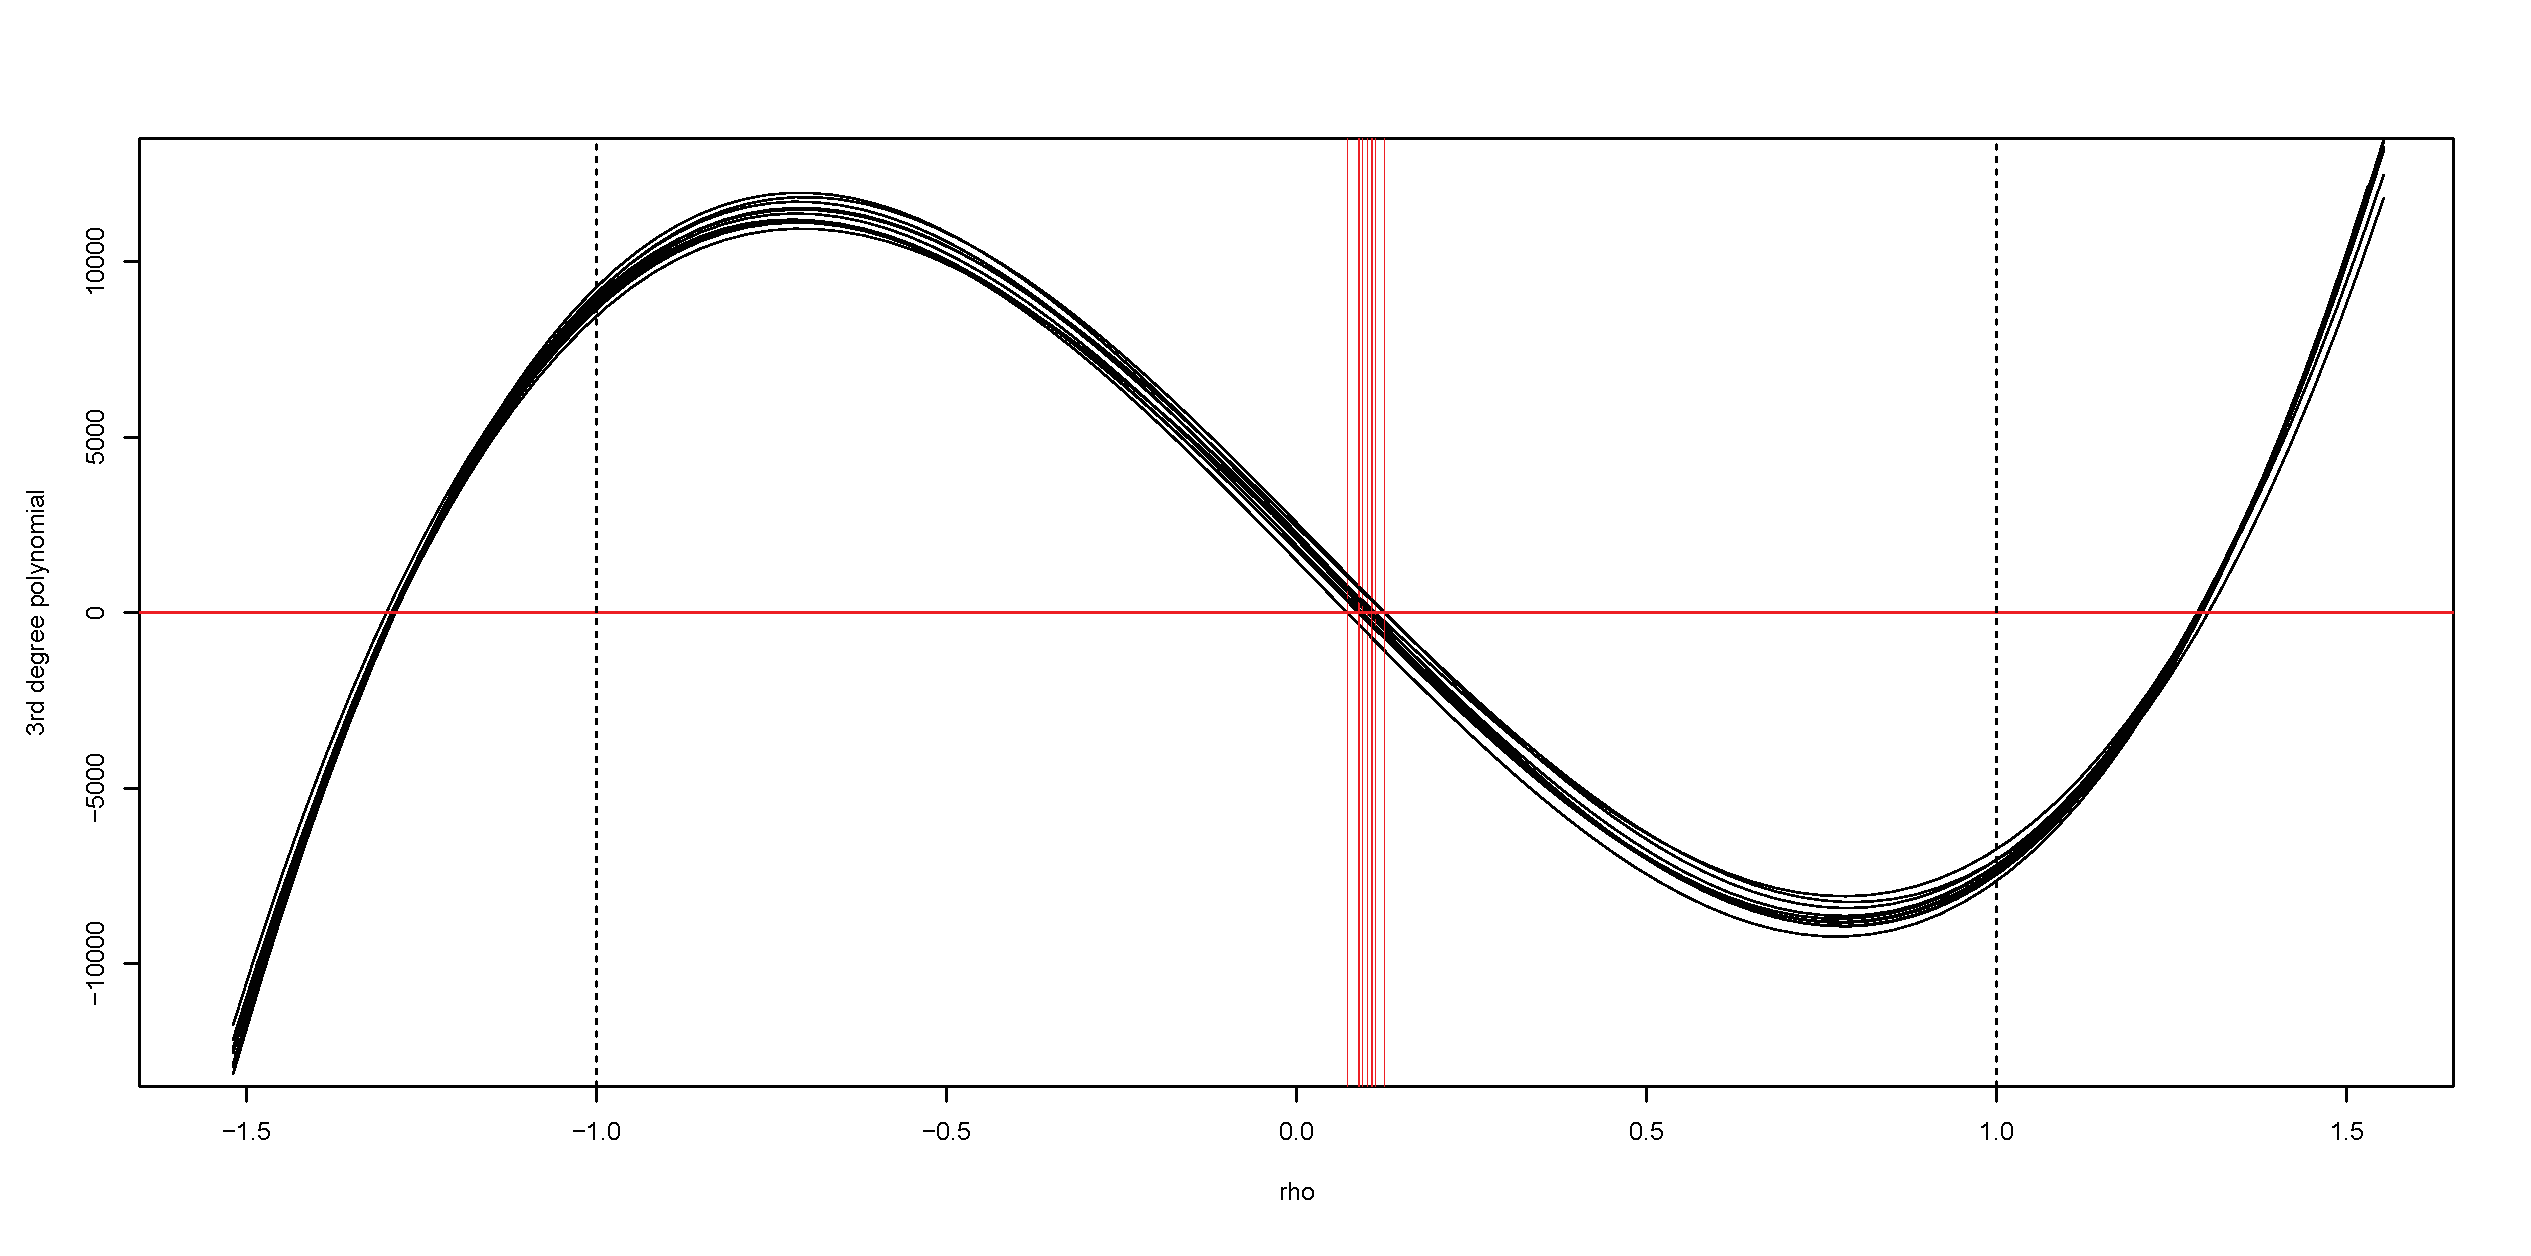
\includegraphics[width=\textwidth]{3rd_poly.eps}
\caption{The third degree polynomial in (\ref{nk_n_rho}) for $10$ different generated data. The red veertical line shows $\widehat{\rho}$.} \label{3rd_poly}
\end{figure}

\section{Details on Additional Simulations\label{suppsimul}}

\subsection{Simulations with Proportional and Size-proportional Weights}

Here we consider $C_1=500,  C_2=250 ,C_3=250, C_4= 500$, and $n_1=5,n_2= 10,n_3= 10,n_4=  5$. Parameters are set to $\mu=0$, $\sigma=2$ and $\rho=(0.1,0.5,0.8)$. The data are generated 100 times and the model is fitted using PROC MIXED in SAS (for a single overall intercept). For combining the results from different sub-samples we have used proportional weights and size-proportional weights:
\begin{equation}
\label{weights}
\begin{cases}
\mbox{Prop}=\frac{C_k}{\sum_l C_l}, \\
\mbox{Size.Prop}=\frac{C_kn_k}{\sum_l C_l n_l}.
\end{cases}.
\end{equation}
The results are compared with full likelihood (Table~\ref{table_comp1}). In contrast to the compound-symmetry case, the size-proportional weights show much better results than the proportional weights. Furthermore, the size-proportional weights in the current simulation are identical with the equal weights. The $n_k$'s have a much larger influence in the AR(1) case compared to CS. 
 Figures~\ref{fig_rho1}, \ref{fig_rho2}, and \ref{fig_rho3} make the comparisons easier.
\begin{table}[t]
\centering
\caption{Comparing proportional, size-proportional and iterated optimal weights with full likelihood for AR(1) covariance structure.}
\label{table_comp1}
 \resizebox{\textwidth}{!}{%
\begin{tabular}{clcccccc}
  \hline\hline
 &&$\widehat{\mu}$ & Sd & $\widehat{\rho}$ & Sd & $\widehat{\sigma}^2$ & Sd \\
 \hline
& Prop. & -0.00190 & 0.01615 & 0.10027 & 0.01158 & 1.99642 & 0.03002 \\
  $\rho=0.1$ & Size.Prop.& -0.00207 & 0.01538 & 0.10024 & 0.01080 & 1.99793 & 0.02853 \\
&It.Opt.  & -0.00206 & 0.01538 & 0.10024 & 0.00993 & 1.99792 & 0.02850\\
&ML   & -0.00207 & 0.01538 & 0.10032 & 0.01078 & 1.99793 & 0.02850 \\
  \hline
& Prop.    & -0.00212 & 0.02221 & 0.49966 & 0.00954 & 2.00349 & 0.03652 \\
  $\rho=0.5$ & Size.Prop& -0.00155 & 0.02156 & 0.49955 & 0.00898 & 2.00257 & 0.03494 \\
  &It.Opt.&  -0.00168 & 0.02149  &0.49956 & 0.00826 & 2.00265 & 0.03486\\
 &ML  & -0.00170 & 0.02150 & 0.49986 & 0.00896 & 2.00259 & 0.03488 \\
    \hline
  & Prop. & 0.00195 & 0.02890 & 0.79923 & 0.00549 & 1.99529 & 0.04989 \\
 $\rho=0.8$ &Size.Prop& 0.00234 & 0.02904 & 0.79911 & 0.00530 & 1.99542 & 0.04907 \\
  &It.Opt.& 0.00213 &0.02855& 0.79915& 0.00486&1.99538& 0.04859\\
&ML   & 0.00212 & 0.02855 & 0.79937 & 0.00527 & 1.99519 & 0.04861 \\
   \hline\hline
\end{tabular}}
\end{table}

\begin{figure}[ht!]
\centering
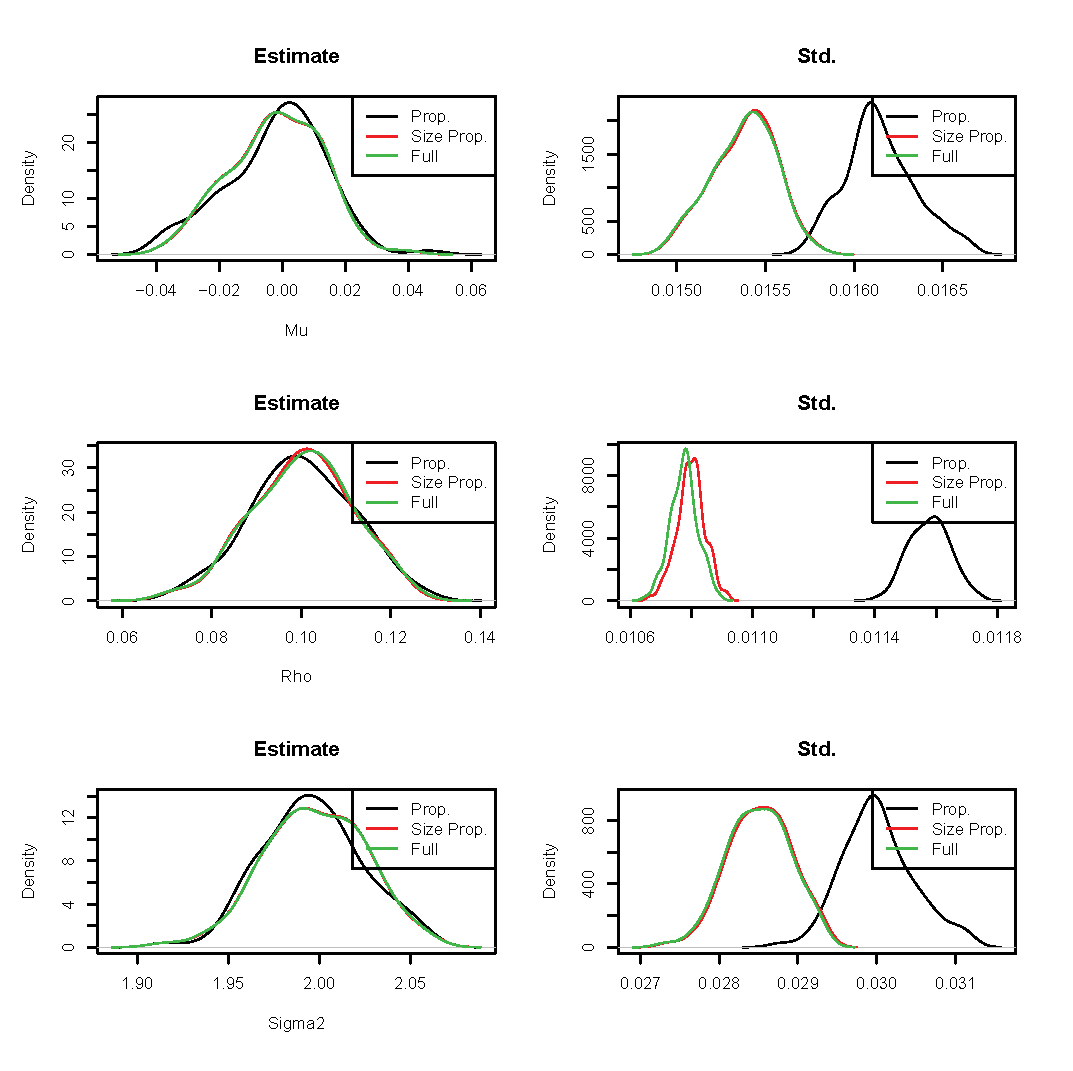
\includegraphics[width=\textwidth]{rho1.eps}
\caption{Comparing proportional and size-proportional weights with full likelihood for $100$ replications with $\mu=0$, $\sigma^2=2$ and $\rho=0.1$.} \label{fig_rho1}
\end{figure}

\begin{figure}[ht!]
\centering
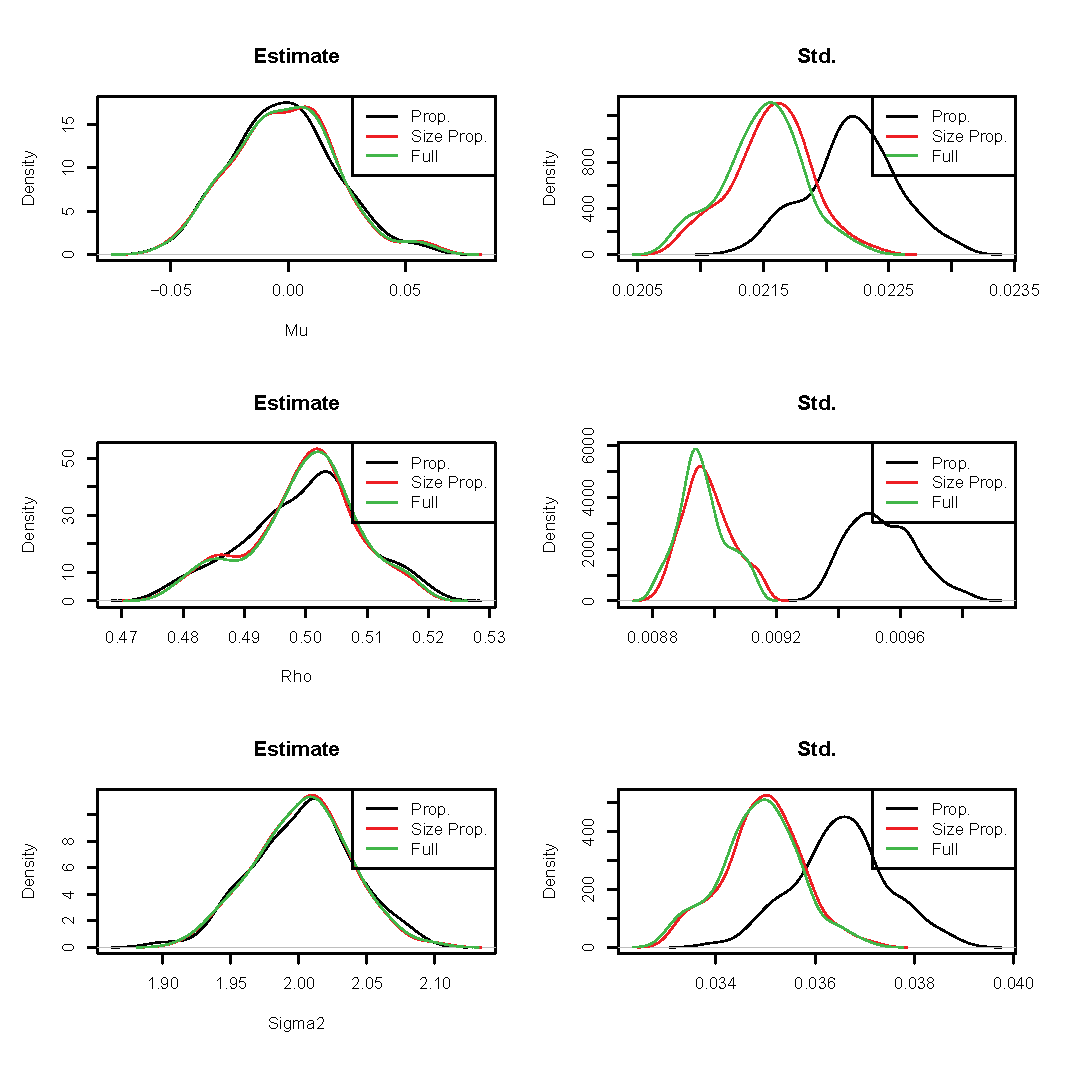
\includegraphics[width=\textwidth]{rho2.eps}
\caption{Comparing proportional and size-proportional weights with full likelihood for $100$ replications with $\mu=0$, $\sigma^2=2$ and $\rho=0.5$.} \label{fig_rho2}
\end{figure}

\begin{figure}[ht!]
\centering
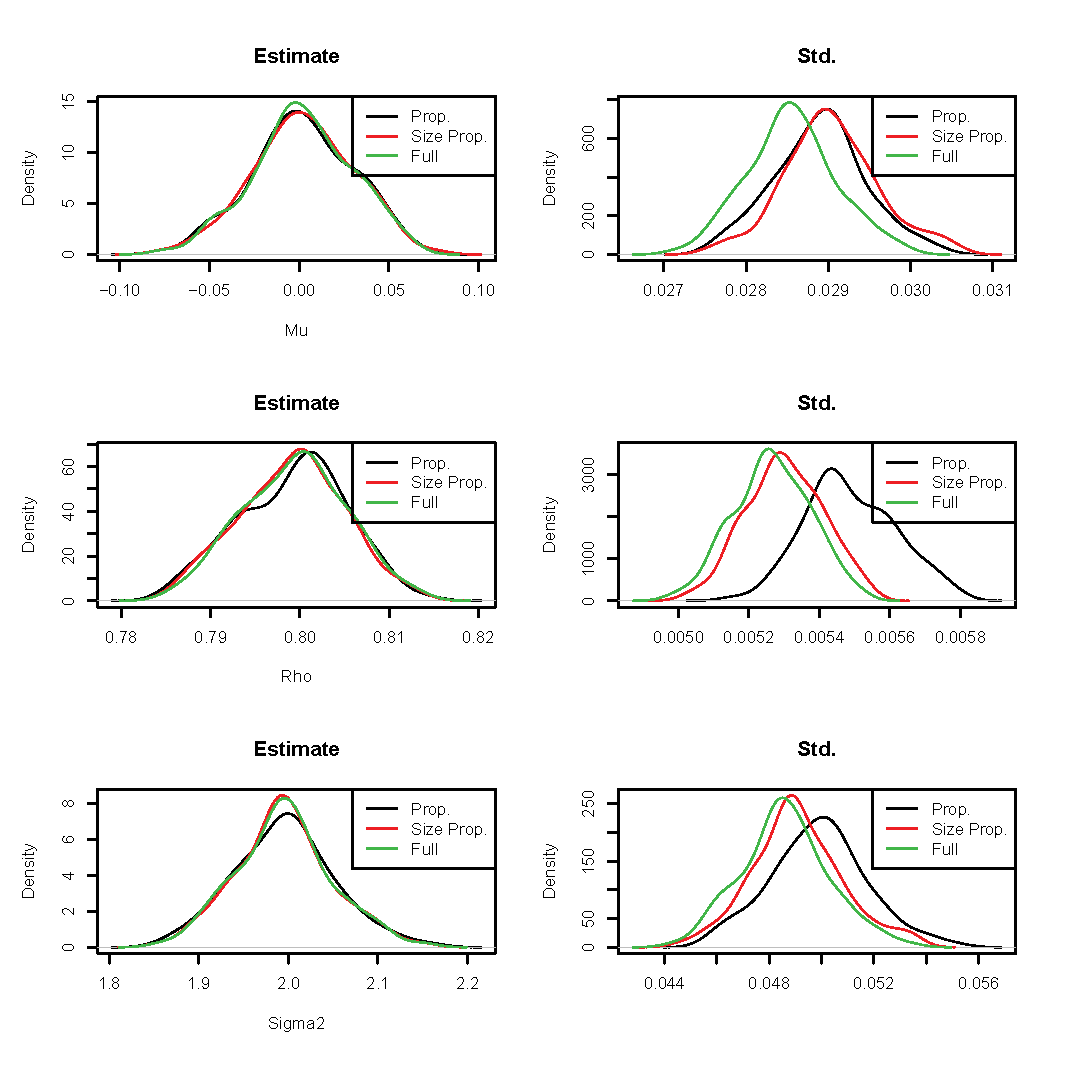
\includegraphics[width=\textwidth]{rho3.eps}
\caption{Comparing proportional and size-proportional weights with full likelihood for $100$ replications with $\mu=0$, $\sigma^2=2$ and $\rho=0.8$.} \label{fig_rho3}
\end{figure}

\subsection{Simulations with Proportional and Size-proportional Weights: $\rho$ near 0/1}

We now present a comparison between proportional and size-proportional weights. We see that,  for $\rho$'s near $1$ (i.e., near CS), size-proportional weights are worse than proportional weights.

We consider $c_1=500$,  $c_2=250$, $c_3=250$, $c_4= 500$, and $n_1=5$, $n_2= 10$, $n_3= 10$, $n_4=  5$. Parameters are set as $\mu=0$, $\sigma=2$ and $\rho\in\{0.01,0.2,0.5,0.8,0.9,0.95,0.99\}$. The data are generated 100 times and the model is fitted using PROC MIXED in SAS (for a single overall intercept). For combining results from different sub-samples we have used proportional weights and size-proportional weights as in (\ref{weights}). The results are compared with full likelihood results.

In Figure~\ref{fig_rho1b}, for $\rho=0.99$ and $0.95$, the size-proportional weights perform  worse than the proportional weights. This is expected, because in this case AR(1) approaches CS. This result is clearer in the left panel of Figure~\ref{fig_rho1b}, where the standard deviations are shown. For $\rho$'s near $1$, the proportional weights are as efficient as  full likelihood, while as $\rho$ moves further from $1$ this would happen for size-proportional weights.

Figure~\ref{fig_rho2b} shows this phenomenon more clearly, as for some selected $\rho$'s ($0.01,0.5,0.95$) the density plot for all $100$ simulated datasets is plotted rather than a  boxplot. The size-proportional weights are better than proportional weights if $\rho$ is not very close to $1$. As soon as $\rho$ becomes $0.95$ or $0.99$, the size-proportional weights become worse.


\begin{figure}[ht!]
\centering
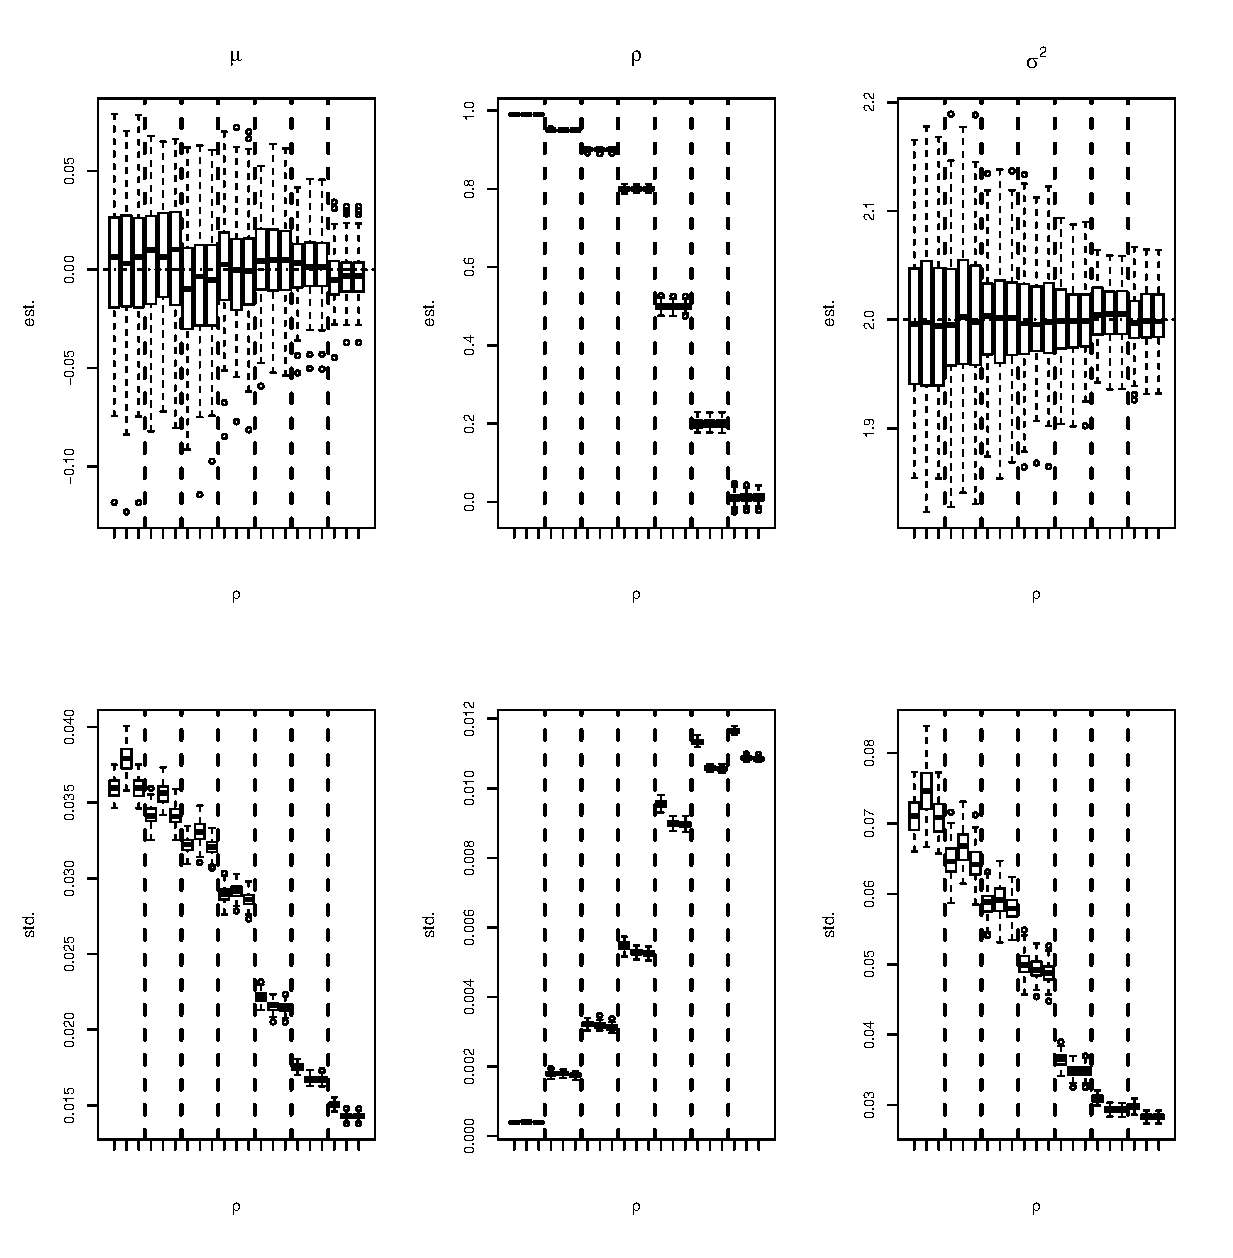
\includegraphics[angle=270]{comp_rho.eps}
\caption[Simulation study. Boxplots comparing proportional and size-proportional weights with full likelihood for $100$ replications with $\mu=0$, $\sigma^2=2$ and $\rho=0.99,0.95,0.9,0.8,0.5,0.2,0.01$]{Simulation study. Boxplots comparing proportional and size-proportional weights with full likelihood for $100$ replications with $\mu=0$, $\sigma^2=2$ and $\rho=0.99,0.95,0.9,0.8,0.5,0.2,0.01$. In every section of the boxplots (which are separated by dashed lines) the first out of three represents the proportional weights, the middle of is size-propotional weights and the one on the right shows the results for the full likelihood. The first row presents the estimates while the second row shows the standard deviations of these estimates.} \label{fig_rho1b}
\end{figure}
\begin{figure}[ht!]
\centering
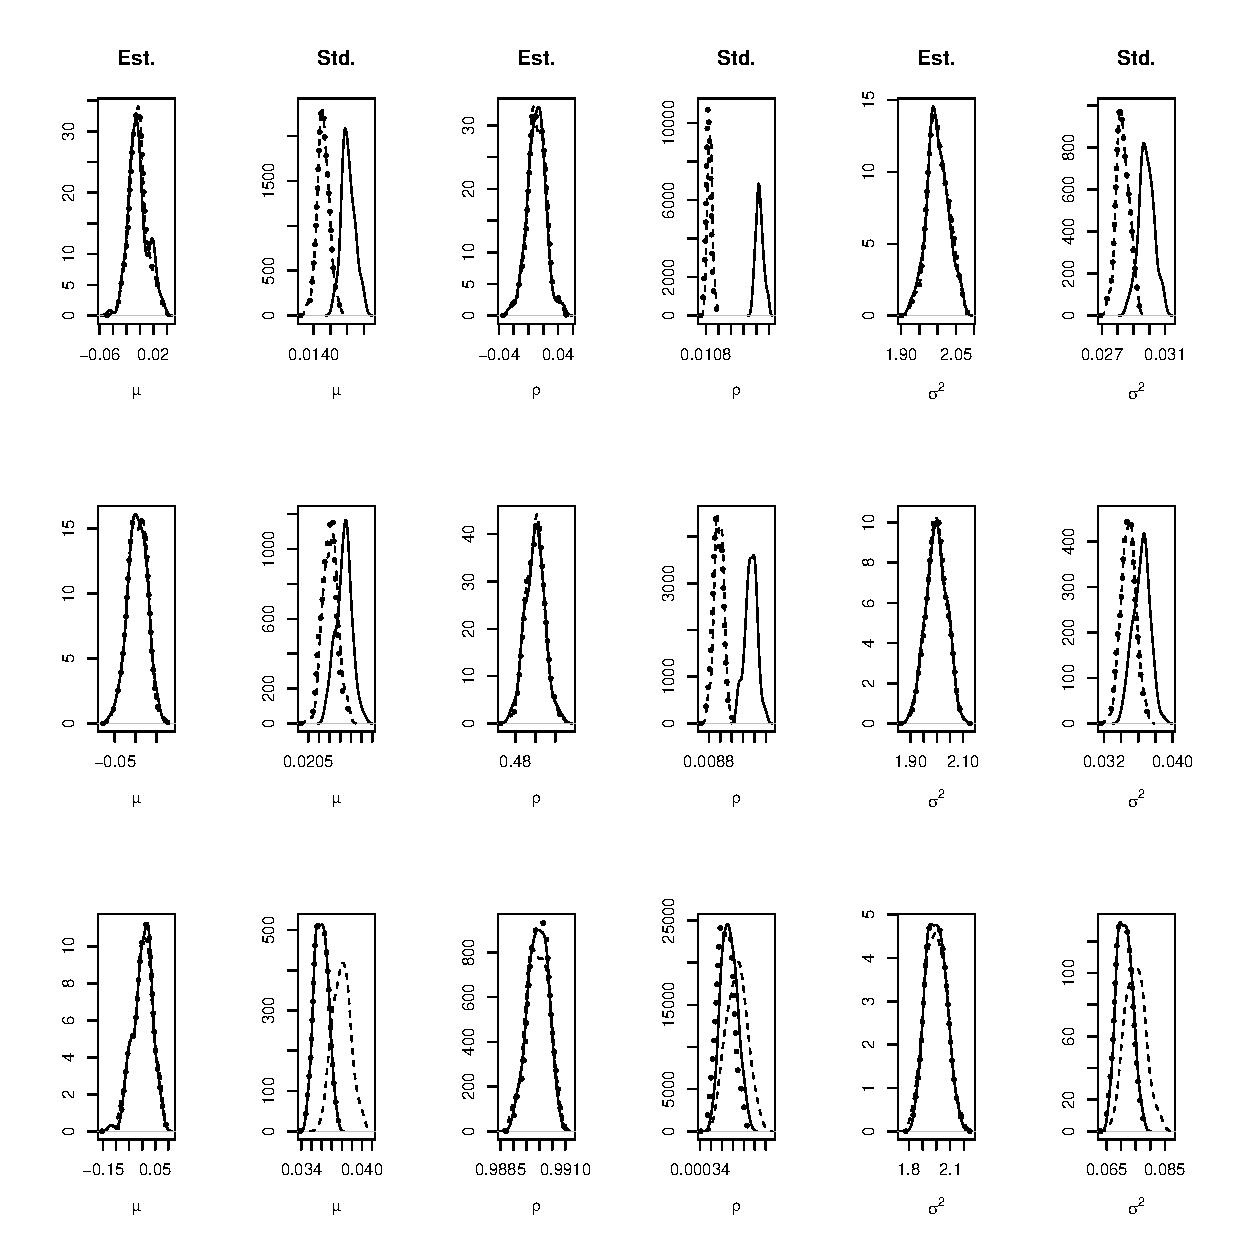
\includegraphics[angle=270]{comp_rho2.eps}
\caption[Simulation study. Comparing proportional, size-proportional and full likelihood results via their empirical density for the 100 replications]{Simulation study. Comparing proportional, size-proportional and full likelihood results via their empirical density for the 100 replications. In all of the figures $\mu=0$ and $\sigma^2=2$. The first row is for $\rho=0.01$, the middle one is for $\rho=0.5$ and last one corresponds to $\rho=0.99$. In each figure the ticker dotted line corresponds to full likelihood, the dashed line is for size-proportional weights and the solid line is for proportional weights.} \label{fig_rho2b}
\end{figure}


\subsection{Simulations With Optimal Weights}

Given the  covariance matrix of the parameter estimators, finding the optimal weights is straightforward, but in practice the unknown parameters therein need to be estimated.  Here we compare the iterative weights with size-proportional weights and ML. See Figures \ref{fig_rho1_opt}, \ref{fig_rho2_opt}, \ref{fig_rho3_opt}, and Table \ref{table_comp1}.
As expected, the optimal weights lead to estimates very close to the MLE; the difference between them being numerical. 

Size-proportional weights are used as the initial weights to begin the iterative procedure. One interesting outcome of this simulation is that the iterative procedure always converged after just one iteration. This means, iterated optimal weights are just like the approximated optimal weights, but there, instead of using $\widehat{\theta}_k$ from each sub-sample, one may use $\tilde{\theta}$ obtained from all sub-samples using a non-optimal but good weight.

\begin{figure}[ht!]
\centering
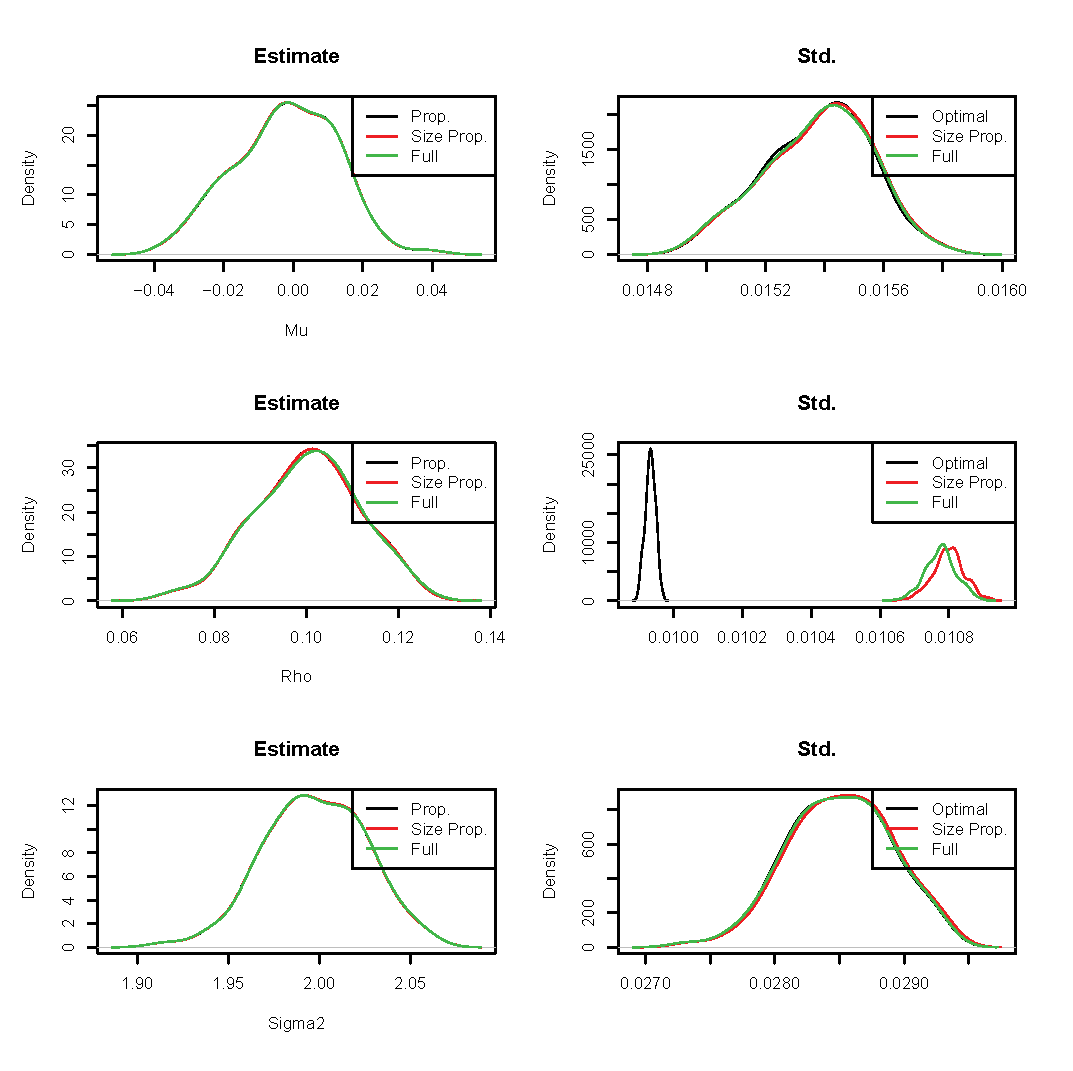
\includegraphics[width=\textwidth]{rho1_opt.eps}
\caption{Comparing iterated optimal and size-proportioanl weights with full likelihood for $100$ replications with $\mu=0$, $\sigma^2=2$ and $\rho=0.1$.} \label{fig_rho1_opt}
\end{figure}

\begin{figure}[ht!]
\centering
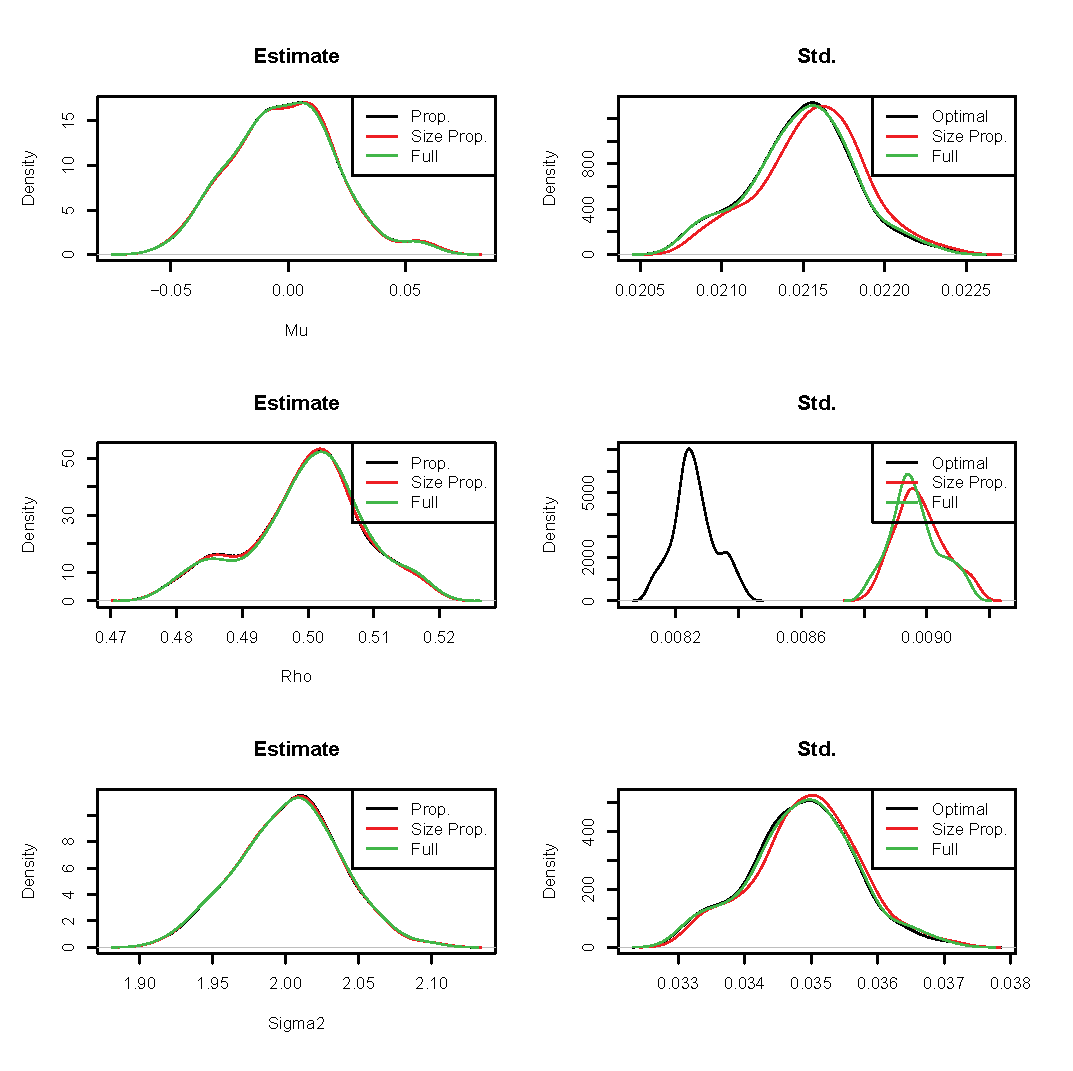
\includegraphics[width=\textwidth]{rho2_opt.eps}
\caption{Comparing iterated optimal and size-proportioanl weights with full likelihood for $100$ replications with $\mu=0$, $\sigma^2=2$ and $\rho=0.5$.} \label{fig_rho2_opt}
\end{figure}

\begin{figure}[ht!]
\centering
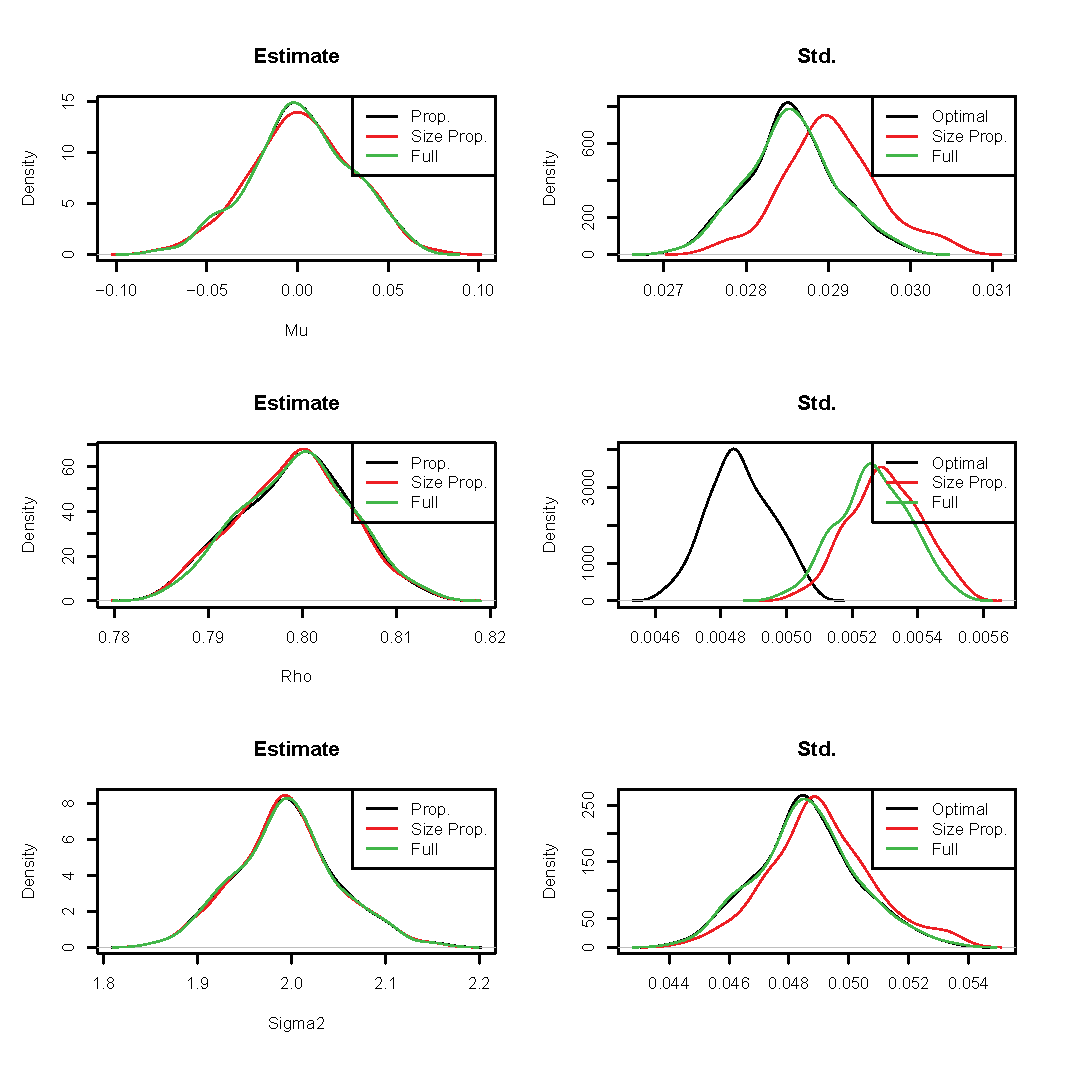
\includegraphics[width=\textwidth]{rho3_opt.eps}
\caption{Comparing iterated optimal and size-proportioanl weights with full likelihood for $100$ replications with $\mu=0$, $\sigma^2=2$ and $\rho=0.8$.} \label{fig_rho3_opt}
\end{figure}


\subsection{Simulations on Computation  Time}
Here, some summary tables are presented to summarize the results which are already presented via figures earlier. Furthermore, a table and a figure are added to compare computation time for closed form solutions to numerical ones.

In each table the mean of the estimated parameter and its standard deviation using the $100$ replications are given, together with the standard deviation of those 100 numbers (in parentheses). If $\theta$ is the parameter of interest, $\widehat{\theta}$ is its estimate and $\theta_0$ is its real value, then the MSE is computed as follows:
\begin{equation}
\label{MSE}
\mathrm{MSE}(\widehat{\theta})=\frac{1}{100}\sum_{i=1}^{100} (\widehat{\theta}-\theta_0)^2.
\end{equation}
Table~\ref{sim_mu} summarizes the results for $\mu$. The sample splitting estimates are computed using proportional and size-proportional (identical to equal weights in this case) weights. The results using the full sample are also given. The third column in Table~\ref{sim_mu} presents the averaged (over 100 replications) estimated $\mu$ and its standard deviation. The fourth column presents the averaged estimated standard deviation for $\widehat{\mu}$ (over 100 replications) and its standard deviation. The last column shows the MSE computed using (\ref{MSE}) for $\mu_0=1$. Tables~\ref{sim_rho} and \ref{sim_sigma2} shows the same results for $\rho$ and $\sigma^2$ ($\sigma^2_0=2$), respectively.

Table~\ref{comp_time} compares the computation time 
between closed-form and interative methods.  The closed-form solutions are implemented in R and for the numerical methods the MIXED procedure in SAS is used, with error covariance structure set to AR(1).

The data are generated using $n=10$ for all clusters, with $c$ is varying from 100 to 1000000. Therefore, the design is balanced and the point of this comparison is to see how the computation time is reduced in each split.

As one may see in Table~\ref{comp_time} and Figure~\ref{fig_comp_time}, using closed form solutions  significantly reduces the computation time. This means, as well as the computation time reduction due to splitting the data, using closed form solutions within each split the computation time reduction is also huge: for example, for a million clusters, the reduction is from  almost one hour to less than 5 seconds. Figure~\ref{fig_comp_time} shows that computation time using closed form solution changes linearly with the number of clusters, while this will be exponential using an iterative solution.

To assess the effect of the overall size of the dataset, the model is fitted to two concatenated copies of the same set. Computation time results are presented in Table~\ref{comp_time} and Figure~\ref{fig_comp_time}.  The data are generated with $\mu=0$, $\sigma^2=2$, and $\rho=0.25$.
\begin{table}[ht]
\centering
\caption[Simulation study. Estimating $\mu$ and its standard deviation]{Simulation study. Estimating $\mu$ and its standard deviation. The mean (standard deviation) of the $100$ replications are given together with mean squared errors for $\rho=0.01,0.2,0.5,0.8,0.9,0.99$ using proportional and size-proportional weights comparing with the full likelihood results.}
\label{sim_mu}

\vspace*{2mm}

\begin{tabular}{cllcccc}
\hline\hline
$\rho_0$&method & mean($\widehat{\mu}$) (s.d.)  & mean(s.e.($\widehat{\mu}$)) (s.d.)  & MSE$\times 10^4$ \\
  \hline
  &Prop. & -0.00271 (0.01462) & 0.01503 (0.00020) & 2.19000 \\
0.01  &Size Prop. & -0.00277 (0.01320) & 0.01429 (0.00018) & 1.80172 \\
  &Full & -0.00275 (0.01319) & 0.01428 (0.00018) & 1.79828 \\ \hline
  &Prop. & 0.00158 (0.01677) & 0.01752 (0.00025) & 2.81056 \\
0.2   &Size Prop. & 0.00085 (0.01616) & 0.01673 (0.00021) & 2.59147 \\
  &Full & 0.00090 (0.01615) & 0.01672 (0.00021) & 2.58880 \\ \hline
  &Prop. & 0.00391 (0.02244) & 0.02217 (0.00037) & 5.13770 \\
0.5   &Size Prop. & 0.00397 (0.02191) & 0.02155 (0.00035) & 4.91201 \\
  &Full & 0.00396 (0.02182) & 0.02148 (0.00034) & 4.87038 \\ \hline
  &Prop. & 0.00130 (0.02790) & 0.02894 (0.00050) & 7.72450 \\
0.8   &Size Prop. & -0.00049 (0.02710) & 0.02912 (0.00045) & 7.27464 \\
  &Full & 0.00053 (0.02713) & 0.02862 (0.00045) & 7.29130 \\ \hline
  &Prop. & -0.00828 (0.03006) & 0.03221 (0.00056)&  9.63393 \\
0.9   &Size Prop. & -0.00727 (0.03145) & 0.03306 (0.00070) & 10.3224 \\
  &Full & -0.00803 (0.02998) & 0.03207 (0.00057) & 9.54258 \\ \hline
  &Prop. & 0.00162 (0.03663) & 0.03597 (0.00064) & 13.3123e \\
0.99   &Size Prop. & -0.00007 (0.03930) & 0.03797 (0.00088) & 15.2876 \\
  &Full & 0.00156 (0.03666) & 0.03597 (0.00064) &  13.3305 \\
   \hline
\hline
\end{tabular}
\end{table}


\begin{table}[ht]
\centering
\caption[Simulation study. Estimating $\rho$ and its standard deviation]{Simulation study. Estimating $\rho$ and its standard deviation. The mean (standard deviation) of the $100$ replications are given together with mean squared errors for $\rho=0.01,0.2,0.5,0.8,0.9,0.99$ using proportional and size-proportional weights comparing with the full likelihood results.}
\label{sim_rho}

\vspace*{2mm}
 \resizebox{\textwidth}{!}{%
\begin{tabular}{lllcccc}
\hline\hline
$\rho_0$&method & mean($\widehat{\rho}$) (s.e.)  & mean(s.e.($\widehat{\rho}$)) (s.e.)  & MSE \\
  \hline
  &Prop. & 0.01077 (0.01237) & 0.01165 (0.00006) &  1.52178e-04 \\
  0.01&Size Prop. & 0.01115 (0.01200) & 0.01087 (0.00004) & 1.43974e-04 \\
  &Full & 0.01123 (0.01203) & 0.01084 (0.00004) & 1.44675e-04 \\  \hline
  &Prop. & 0.19960 (0.01213) & 0.01133 (0.00007) & 1.45806e-04  \\
 0.2 &Size Prop. & 0.19973 (0.01145) & 0.01058 (0.00005) &  1.29974e-04 \\
  &Full& 0.19986 (0.01142) & 0.01056 (0.00005) & 1.29174e-04 \\  \hline
  &Prop. & 0.49956 (0.00963) & 0.00954 (0.00011) & 9.19119e-05 \\
0.5  &Size Prop. & 0.49965 (0.00904) & 0.00898 (0.00008) & 8.11057e-05 \\
  &Full & 0.49990 (0.00904) & 0.00896 (0.00008) & 8.08877e-05 \\  \hline
  &Prop. & 0.79973 (0.00541) & 0.00548 (0.00012) & 2.90660e-05 \\
0.8  &Size Prop & 0.79990 (0.00483) & 0.00529 (0.00009) & 2.31132e-05 \\
  &Full & 0.80018 (0.00489) & 0.00525 (0.00009) &  2.36726e-05 \\  \hline
  &Prop. & 0.90017 (0.00286) & 0.00321 (0.00008) & 8.14862e-06 \\
0.9  &Size Prop. & 0.90013 (0.00297) & 0.00318 (0.00008) & 8.76257e-06 \\
  &Full & 0.90040 (0.00292) & 0.00312 (0.00008) & 8.60114e-06 \\  \hline
  &Prop. & 0.98994 (0.00038) & 0.00039 (0.00001) & 1.45292e-07 \\
0.99  &Size Prop. & 0.98992 (0.00042) & 0.00041 (0.00002) & 1.77848e-07 \\
  &Full & 0.98997 (0.00037) & 0.00039 (0.00001) & 1.37289e-07  \\
   \hline\hline
\end{tabular}}
\end{table}


\begin{table}[ht]
\centering
\caption[Simulation study. Estimating $\sigma^2$ and its standard deviation]{Simulation study. Estimating $\sigma^2$ and its standard deviation. The mean (standard deviation) of the $100$ replications are given together with mean squared errors for $\rho=0.01,0.2,0.5,0.8,0.9,0.99$ using proportional and size-proportional weights comparing with the full likelihood results.}
\label{sim_sigma2}

\vspace*{2mm}
 \resizebox{\textwidth}{!}{%
\begin{tabular}{lllcccc}
\hline\hline
$\rho_0$&method& mean($\widehat{\sigma}^2$) (s.e.)  & mean(s.e.($\widehat{\sigma}^2$)) (s.e.)  & MSE \\
  \hline
  &Prop. & 1.99964 (0.02960) & 0.02981 (0.00049) & 8.67280e-04 \\
0.01  &Size Prop. & 2.00165 (0.02836) & 0.02834 (0.00040) & 7.98842e-04 \\
  &Full & 2.00167 (0.02832) & 0.02832 (0.00040) & 7.97002e-04 \\   \hline
  &Prop. & 2.00581 (0.02907) & 0.03093 (0.00055) & 8.70077e-04  \\
0.2  &Size Prop. & 2.00484 (0.02778) & 0.02936 (0.00044) & 7.87298e-04 \\
  &Full & 2.00473 (0.02772) & 0.02933 (0.00044) & 7.83248e-04 \\   \hline
  &Prop. & 1.99783 (0.03860) & 0.03638 (0.00097) & 1.47960e-03 \\
0.5  &Size Prop. & 1.99890 (0.03747) & 0.03488 (0.00085) & 1.39116e-03 \\
  &Full & 1.99897 (0.03748) & 0.03481 (0.00085) & 1.39152e-03 \\   \hline
  &Prop. & 2.00013 (0.04900) & 0.05002 (0.00166) & 2.37744e-03 \\
0.8  &Size Prop. & 2.00136 (0.04423) & 0.04930 (0.00137) & 1.93881e-03 \\
  &Full & 2.00101 (0.04569) & 0.04880 (0.00142) & 2.06754e-03 \\   \hline
  &Prop. & 2.00122 (0.05767) & 0.05872 (0.00196) & 3.29407e-03 \\
0.9  &Size Prop. & 2.00089 (0.06037) & 0.05915 (0.00230) & 3.60829e-03 \\
  &Full & 2.00115 (0.05876) & 0.05793 (0.00198) &  3.41986e-03 \\   \hline
  &Prop. & 1.99683 (0.06941) & 0.07117 (0.00254) & 4.77911e-03\\
0.99  &Size Prop. & 1.99527 (0.07598) & 0.07484 (0.00344) & 5.73813e-03 \\
  &Full & 1.99641 (0.06940) & 0.07093 (0.00253) & 4.78099e-03 \\
   \hline\hline
\end{tabular}}
\end{table}


\addtolength{\tabcolsep}{-.9mm}

\begin{table}[ht]
\centering
\caption[Simulation study. The computation time]{Simulation study. The computation time for a sample with $n=10$ and $c=$1e+02, 1e+03, 1e+04, 5e+04, 1e+05, 3e+05, 5e+05, 7e+05, 9e+05, 1e+06. The closed form solution is obtained by implementing the results of this paper in R, and the numerical solution is obtained using PROC MIXED in SAS to estimate a repeated measurement model with AR(1) covariance structure.}
\label{comp_time}

\vspace*{2mm}
 \resizebox{\textwidth}{!}{%
\begin{tabular}{lcccccccccc}
  \hline\hline
 time (s) & 1e+02 &1e+03&1e+04& 5e+04& 1e+05& 3e+05 &5e+05 &7e+05& 9e+05 &1e+06\\
   \hline
  Closed form & 0.00 & 0.00 & 0.03 & 0.23 & 0.34 & 1.45 & 2.07 & 3.37 & 4.40 & 4.89 \\
  Numerical & 0.08 & 0.13 & 1.04 & 10.45 & 34.74 & 268.96 & 770.74 & 1611.43 & 2724.31 & 3399.47 \\
   \hline
\hline
\end{tabular}}
\end{table}


\addtolength{\tabcolsep}{.9mm}


\begin{figure}[t]
\centering
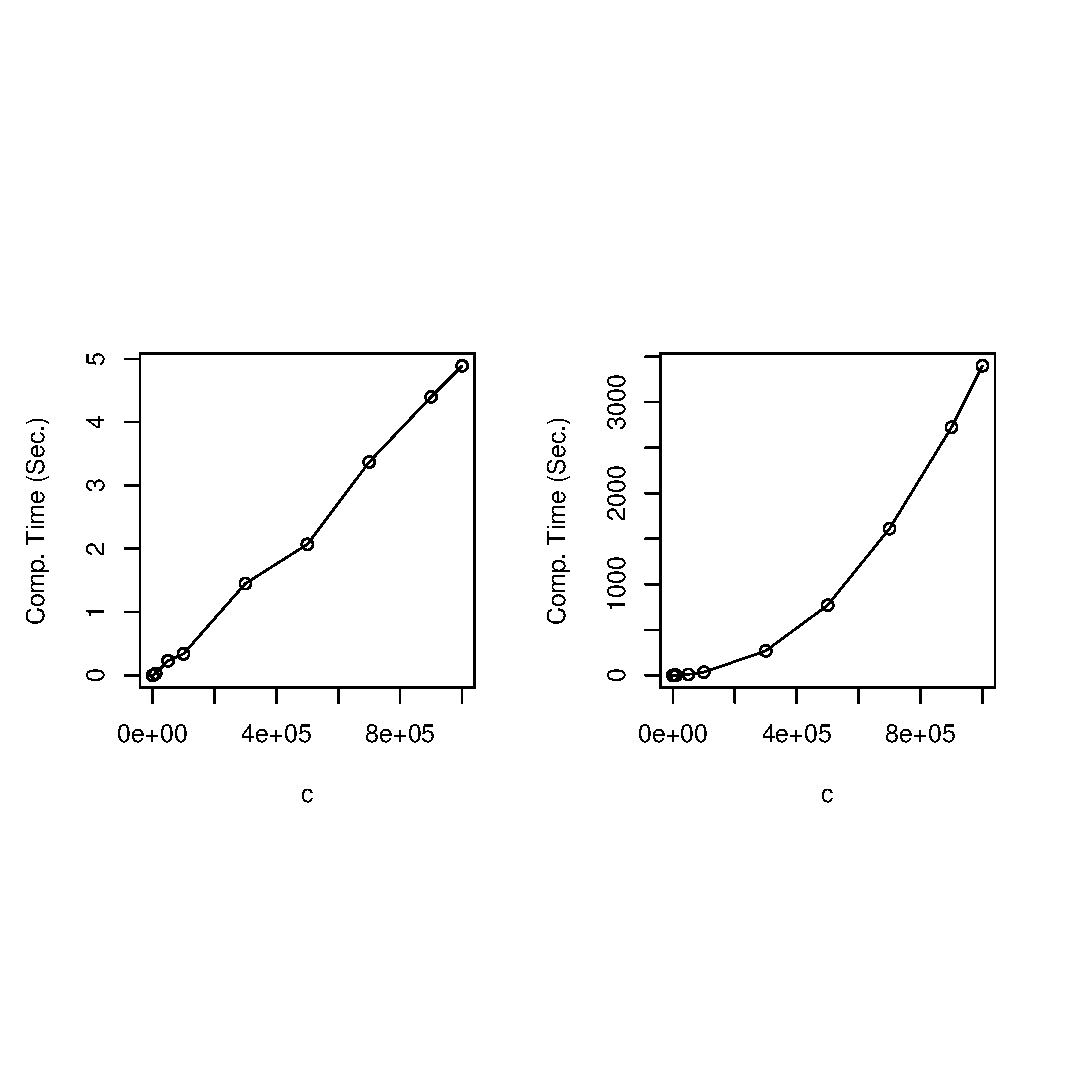
\includegraphics[scale=1, trim= 0cm 4cm 0cm 4cm]{comp_time.eps}
\caption[Simulation study. Comparing computation time using closed form and numerical solutions]{Simulation study. Comparing computation time using closed form (left) and numerical (right) solutions. The horizontal axis shows number of clusters ($c$) and the vertical axis shows the computation time in seconds.} \label{fig_comp_time}
\end{figure}

\section{Details on PANSS Data Analysis}\label{suppdata}
\vspace{-3.5mm}
As one may see from Table~\ref{PANSSTab_freq}, by far the majority of the study subjects have complete data and hence belong to the first pattern.

 Figure~\ref{fig_all_first} presents boxplots for the entire set of data, for the subjects from the first pattern only, and for various split samples. 


\begin{table}[ht!]
\centering
\caption{PANSS data. Number of clusters in each trial for each cluster pattern.}
\label{PANSSTab_freq}\vspace*{2mm}
 \resizebox{\textwidth}{!}{%
\begin{tabular}{rcccccccccccccccc}
\hline\hline
 & &&&&&&&&&&  \multicolumn{5}{c}{Trial} &  \\
  \cline{12-16}
$n$ & \multicolumn{10}{c}{Pattern}  & FIN-1 & FRA-3 & INT-2 & INT-3 & INT-7 &Total  \\
  \hline
 &  $\ast$& $\ast$& $\cdot$& $\cdot$& $\cdot$& $\cdot$& $\cdot$& $\cdot$&  $\cdot$&  $\cdot$&  17 & 8 & 71 & 43 & 3 & 142 \\
  2 &  $\ast$& $\cdot$& $\ast$& $\cdot$& $\cdot$& $\cdot$& $\cdot$& $\cdot$&  $\cdot$&  $\cdot$ & 0 & 0 & 2 & 0 & 1 & 3 \\
   &  $\ast$& $\cdot$& $\cdot$& $\cdot$& $\ast$& $\cdot$& $\cdot$& $\cdot$&  $\cdot$&  $\cdot$ & 0 & 0 & 1 & 0 & 0 & 1 \\ \hline
   &  $\ast$& $\ast$& $\ast$& $\cdot$& $\cdot$& $\cdot$& $\cdot$& $\cdot$&  $\cdot$&  $\cdot$ & 8 & 4 & 83 & 41 & 7 & 143 \\
  3 &  $\ast$& $\cdot$& $\ast$& $\cdot$& $\ast$& $\cdot$& $\cdot$& $\cdot$&  $\cdot$&  $\cdot$ & 0 & 0 & 2 & 0 & 0 & 2 \\
   &  $\ast$& $\ast$& $\cdot$& $\cdot$& $\ast$& $\cdot$& $\cdot$& $\cdot$&  $\cdot$&  $\cdot$ & 1 & 0 & 3 & 1 & 0 & 5 \\ \hline
   &  $\ast$& $\ast$& $\ast$& $\cdot$& $\ast$& $\cdot$& $\cdot$& $\cdot$&  $\cdot$&  $\cdot$ & 11 & 0 & 85 & 66 & 5 & 167 \\
   &  $\ast$& $\cdot$& $\ast$& $\cdot$& $\ast$& $\cdot$& $\ast$& $\cdot$&  $\cdot$&  $\cdot$ & 0 & 0 & 1 & 0 & 1 & 2 \\
  4 &  $\ast$& $\cdot$& $\ast$& $\cdot$& $\ast$& $\cdot$& $\cdot$& $\ast$&  $\cdot$&  $\cdot$ & 0 & 0 & 1 & 0 & 0 & 1 \\
   &  $\ast$& $\ast$& $\ast$& $\cdot$& $\cdot$& $\cdot$& $\ast$& $\cdot$&  $\cdot$&  $\cdot$ & 0 & 0 & 3 & 0 & 0 & 3 \\
   &  $\ast$& $\ast$& $\ast$& $\ast$& $\cdot$& $\cdot$& $\cdot$& $\cdot$&  $\cdot$&  $\cdot$ & 0 & 4 & 1 & 0 & 0 & 5 \\
   &  $\ast$& $\ast$& $\cdot$& $\ast$& $\cdot$& $\cdot$& $\ast$& $\cdot$&  $\cdot$&  $\cdot$ & 0 & 1 & 0 & 0 & 0 & 1 \\
  &  $\ast$& $\cdot$& $\ast$& $\cdot$& $\cdot$& $\cdot$& $\ast$& $\ast$&  $\cdot$&  $\cdot$ & 0 & 0 & 0 & 0 & 1 & 1 \\ \hline
   &  $\ast$& $\ast$& $\ast$& $\cdot$& $\ast$& $\cdot$& $\ast$& $\cdot$&  $\cdot$&  $\cdot$ & 58 & 0 & 85 & 35 & 6 & 184 \\
   &  $\ast$& $\ast$& $\ast$& $\cdot$& $\ast$& $\cdot$& $\cdot$& $\ast$&  $\cdot$&  $\cdot$ & 0 & 0 & 8 & 0 & 1 & 9 \\
   &  $\ast$& $\ast$& $\cdot$& $\cdot$& $\ast$& $\cdot$& $\ast$& $\ast$&  $\cdot$&  $\cdot$ & 0 & 0 & 6 & 0 & 0 & 6 \\
  5 &  $\ast$& $\ast$& $\ast$& $\cdot$& $\cdot$& $\cdot$& $\ast$& $\ast$&  $\cdot$&  $\cdot$ & 0 & 0 & 8 & 0 & 0 & 8 \\
   & $\ast$& $\cdot$& $\ast$& $\cdot$& $\ast$& $\cdot$& $\ast$& $\ast$&  $\cdot$&  $\cdot$ & 0 & 0 & 3 & 0 & 2 & 5 \\
   & $\ast$& $\cdot$& $\ast$& $\cdot$& $\ast$& $\cdot$& $\cdot$& $\ast$&  $\cdot$&  $\ast$ & 0 & 0 & 1 & 0 & 0 & 1 \\
   & $\ast$& $\ast$& $\ast$& $\ast$& $\ast$& $\cdot$& $\cdot$& $\cdot$&  $\cdot$&  $\cdot$ & 0 & 44 & 0 & 0 & 0 & 44 \\
   & $\ast$& $\ast$& $\cdot$& $\ast$& $\ast$& $\ast$& $\cdot$& $\cdot$&  $\cdot$&  $\cdot$ & 0 & 1 & 0 & 0 & 0 & 1 \\ \hline
   & $\ast$& $\ast$& $\ast$& $\cdot$& $\ast$& $\cdot$& $\ast$& $\ast$&  $\cdot$&  $\cdot$ & 0 & 0 & 986 & 240 & 74 & 1300 \\
   & $\ast$& $\ast$& $\cdot$& $\cdot$& $\ast$& $\cdot$& $\ast$& $\ast$&  $\ast$&  $\cdot$ & 0 & 0 & 1 & 0 & 0 & 1 \\
  6 & $\ast$& $\ast$& $\ast$& $\cdot$& $\cdot$& $\cdot$& $\ast$& $\ast$&  $\cdot$&  $\ast$ & 0 & 0 & 1 & 0 & 0 & 1 \\
   & $\ast$& $\ast$& $\ast$& $\cdot$& $\ast$& $\cdot$& $\ast$& $\cdot$&  $\ast$&  $\cdot$ & 0 & 0 & 1 & 0 & 0 & 1 \\
  & $\ast$& $\ast$& $\ast$& $\cdot$& $\ast$& $\ast$& $\ast$& $\cdot$&  $\cdot$&  $\cdot$ & 0 & 0 & 2 & 0 & 0 & 2 \\
   \hline\hline
\end{tabular}}
\end{table}

\begin{figure}[ht]
\centering
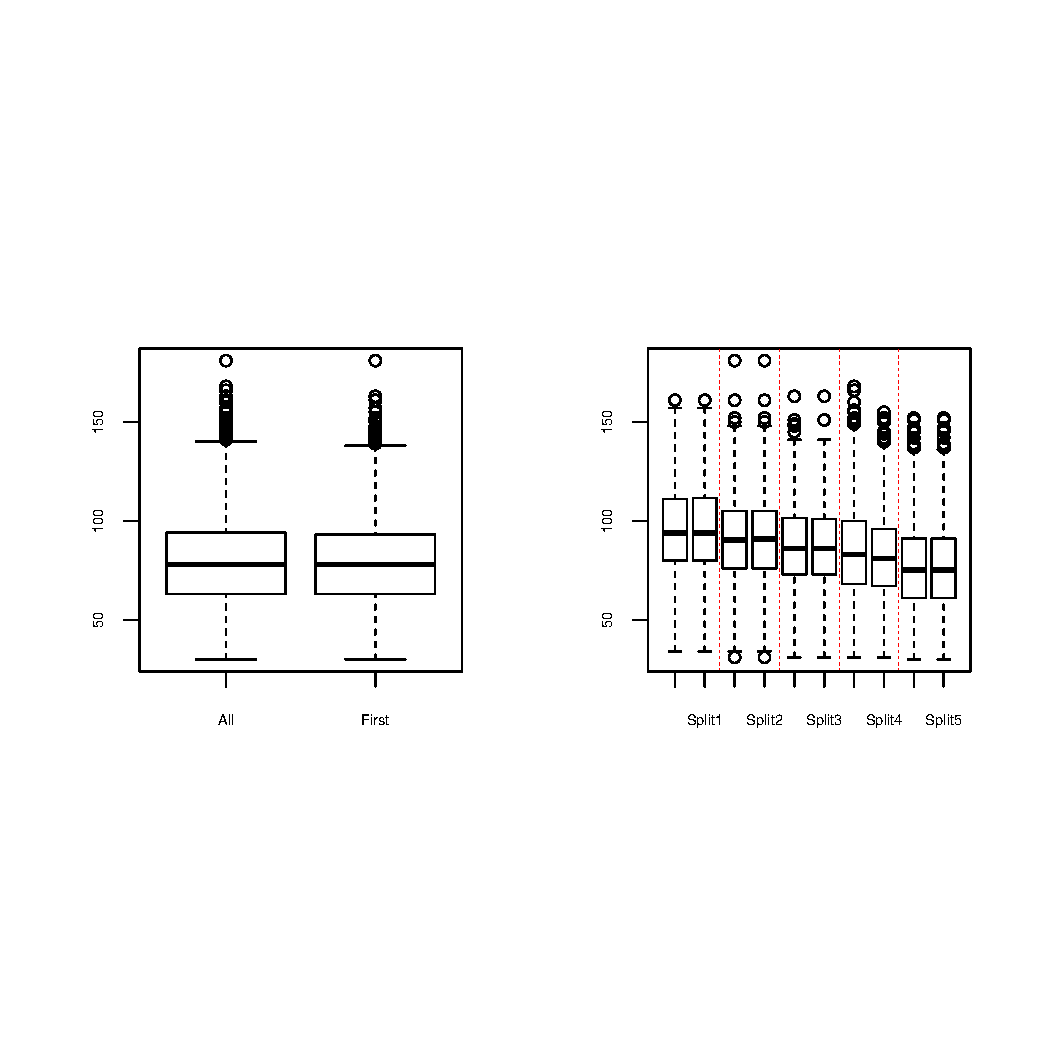
\includegraphics[trim=2cm 5cm 2cm 5cm,scale=1]{all_first.eps}
\caption{PANSS data. Boxplots for the entire set of data, for the subject from the first pattern only, and for various split samples. } \label{fig_all_first}
\end{figure}

To examine the choice of an AR(1) covariance structure, Table~\ref{fig_model_comp} shows three model selection criteria  to compare different error covariance structures. Changing from independence structure ($R=\sigma^2 I$) to compound-symmetry ($R=\sigma^2 I$) the criteria decrease with a large amount, and the same when changing to AR(1). The step to an unstructured covariance does not make a big difference (considering that the unstructured covariance would has $21$ parameters to estimate compared to $2$ parameters in the AR(1) model). Therefore, AR(1) seems to be a good choice.

\begin{table}[t]
\centering
\caption[PANSS data. Comparing different error covariance structures using three model comparison criteria for without trial model]{PANSS data. Comparing different error covariance structures using three model comparison criteria for model (\ref{model_no_trial}) (residual log-likelihood value; AIC; BIC). Three $R$ structures: Ind. : independence structure ($R=\sigma^2 I$), CS: compound-symmetry structure ($R= \sigma^2 I +dJ $), AR(1): AR(1) structure ($R_{ij}=\sigma^2 \rho^{|i-j|}$), UN: unstructured ($R_{ij}=\sigma^2_{ij}$).} \label{fig_model_comp}

\begin{tabular}{lccc}
\hline
\hline
Model&-2 Res.log.lik.&AIC&BIC\\
\hline
Unstructured  &80005.1&80047.1&80164.1\\
AR(1)         &80522.6&80526.6&80537.8\\
Compound symm.&82683.1&82687.1&82698.3\\
Independence  &89546.1&89548.1&89553.7\\
\hline\hline
\end{tabular}
\end{table}

The $95\%$ confidence intervals, accompanying (\ref{model_no_trial}), are presented in Figure~\ref{fig_without_trial}. In order to give more insight in these results, Figure~\ref{fig_without_trial_split} shows the $95\%$ confidence interval in each split, comparing with the full sample splits (the horizontal dashed line in the figure).

The $95\%$ confidence intervals, accompanying (\ref{model_trial}), are presented in Figure~\ref{fig_with_trial}. Figure~\ref{fig_with_trial_split} shows the $95\%$ confidence intervals for the parameter estimates in each split comparing with the full sample estimate (the horizontal dashed-like in the figure.)


\begin{figure}[ht]
\centering
\includegraphics[width=\textwidth]{without_trial.eps}
\caption[PANSS data. $95\%$ confidence intervals for fixed effects and variance components estimates and the standard deviations of these estimates using sample splitting, combined with proportional and size-proportional weights, and full likelihood (without trial model)]{PANSS data. $95\%$ confidence intervals for fixed effects and variance components estimates and the standard deviations of these estimates using sample splitting, combined with proportional (Pr - first) and size-proportional (S-Pr - second) weights, and full likelihood (Fl - third). The dashed horizontal line shows the full likelihood estimate. The model used in here is without trial effect (\ref{model_no_trial}).} \label{fig_without_trial}
\end{figure}

\begin{figure}[ht]
\centering
\includegraphics[width=\textwidth]{without_trial_split_by_split.eps}
\caption[PANSS data. $95\%$ confidence intervals for fixed effects and variance components estimates and the standard deviations of these estimates within each split (without trial model)]{PANSS data. $95\%$ confidence intervals for fixed effects and variance components estimates and the standard deviations of these estimates within each split. The dashed horizontal line shows the full likelihood estimate. The model used in here is without trial effect (\ref{model_trial}).} \label{fig_without_trial_split}
\end{figure}

\begin{figure}[ht]
\centering
\includegraphics[width=\textwidth]{with_trial.eps}
\caption[PANSS data. $95\%$ confidence intervals for fixed effects and variance components estimates and the standard deviations of these estimates using sample splitting, combined with proportional and size-proportional weights, and full likelihood (with trial model)]{PANSS data. $95\%$ confidence intervals for fixed effects and variance components estimates and the standard deviations of these estimates using sample splitting, combined with proportional (Pr - first) and size-proportional (S-Pr - second) weights, and full likelihood (Fl - third). The dashed horizontal line shows the full likelihood estimate. The model used in here is with trial effect (\ref{model_trial}).} \label{fig_with_trial}
\end{figure}


\begin{figure}[ht]
\centering
\includegraphics[width=\textwidth]{with_trial_split_by_split.eps}
\caption[PANSS data. $95\%$ confidence intervals for fixed effects and variance components estimates and the standard deviations of these estimates within each split (with trial model)]{PANSS data. $95\%$ confidence intervals for fixed effects and variance components estimates and the standard deviations of these estimates within each split. The dashed horizontal line shows the full likelihood estimate. The model used in here is with trial effect (\ref{model_trial}).} \label{fig_with_trial_split}
\end{figure}




\section{Fieller's method and Delta method}
\label{app1}

Here, the Fieller's method to construct a confidence interval for (\ref{nf_var_min_cs}) as well as the Delta method  are discussed. The ratio which we require a confidence interval for is:
$$n_f=\frac{\hat{\sigma^2}}{\widehat{\tau} \varepsilon}.$$
Suppose $n_1$ is a small-feasible sub-sampling size chosen to estimate the parameters in the model (e.g., $n_1=5$). From \cite{Iddi2011}, one finds:



\begin{multline}
%\label{cov_sigma2_tau}
\mathrm{Var}  \left(
\begin{array}{c}
\widehat{\sigma^2}\\
\widehat{\tau\varepsilon}
\end{array} \right) =  \\ \frac{2 \sigma^4}{Nn_1(n_1-1)}  \left(
\begin{array}{cc}
n_1 & -\varepsilon \\
-\varepsilon & \varepsilon^2\frac{\sigma^4 + 2(n_1-1) \tau \sigma^2 + n_1 (n_1-1) \tau^2}{\sigma^4}
\end{array} \right) \\ = \left(
\begin{array}{cc}
s_{11} &  s_{12} \\ s_{12} & s_{22}
\end{array} \right).
\end{multline}

The Fieller's confidence interval for (\ref{nf_var_min_cs}) can be calculated following these steps.
\begin{equation}
\begin{aligned}
C_1^2 =&\frac{s_{11}}{\widehat{\sigma^2}^2}, \\
C_2^2=& \frac{s_{22}}{\left(\varepsilon\widehat{\tau}\right)^2},\\
r= & \frac{s_{12}}{\sqrt{s_{11} s_{22}}},\\
A= &C_1^2 + C_2^2 - 2r C_1C_2,\\
B=& t^2 C_1^2 C_2^2 (1-r^2),\\
L=& \frac{\widehat{\sigma^2}}{\varepsilon\widehat{\tau}} \frac{1-z_{\alpha/2}^2 r C_1C_2 - z_{\alpha/2}\sqrt{A-B}}{1-z_{\alpha/2}^2C_2^2},\\
U=& \frac{\widehat{\sigma^2}}{\varepsilon\widehat{\tau}} \frac{1-z_{\alpha/2}^2 r C_1C_2 + z_{\alpha/2}\sqrt{A-B}}{1-z_{\alpha/2}^2C_2^2}.
\end{aligned}
\end{equation}
One may take $n_f=\max\{L,U\}$. Of course, in case were $z_{\alpha/2}^2 C_2^2 <1$, there would be no finite interval. As it was mentioned, one may also use the Delta method as follows:

\begin{equation}
\label{var_delta_method}
\mathrm{Var}(\frac{\widehat{\sigma^2}}{\varepsilon \widehat{\tau}}) \approx \frac{1}{\varepsilon^2 \widehat{\tau}^2} \left( s_{11} - 2 \frac{\sigma^2}{\tau} s_{12} + \frac{\sigma^4}{\tau^2} s_{22} \right).
\end{equation}

\section[Random vertical data splitting for CS]{Random vertical data splitting for compound-symmetry structure}
\label{app2}
Assume a single cluster of size $N$ with multivariate normal distribution and compound-symmetry structure for its covariance matrix, see Section~\ref{sec_CS_effect}. Suppose we take $M_0$ sub-samples of size $n_0$ from this cluster. Following \cite{hoffman2001}, the parameter $\mu$ should be estimated within each sub-sample, $\widehat{\mu}^{(m)}$ ($m=1,\ldots,M_0$) and then the overall estimate can be obtained by averaging these estimates. Furthermore, one needs the within and between sub-samples variabilities to compute the overall variability, see (\ref{mo_cov}).

Within each sub-sample the variance of $\widehat{\mu}^{(m)}$ can be computed using the variance formula for a mean estimator in CS-multivariate normal \cite{Iddi2011} :

\begin{equation}
\label{within}
S_W= \frac{\sigma^2}{n_0} \left[ 1+ (n_0-1) \rho \right ].
\end{equation}
Estimating the between variability requires computing $\mathrm{E}\left\{ (\widehat{\mu}^{(m)} - \bar{\mu})^2 \right\}$, where $\bar{\mu}$ is the average of $\widehat{\mu}^{(m)}$'s ($m=1,\ldots,M_0$). Set $S_m$ as the index of members of sub-sample $m$ and $S_{m'}$ the rest of the sample, then,
\begin{equation*}
\widehat{\mu}^{(m)} - \bar{\mu} = \frac{1}{n_0}\left\{(1-\frac{1}{M_0})\sum_{i\in S_m} y_i - \frac{1}{M_0} \sum_{m=1}^ {M_0} \sum_{i\in S_{m'}} y_i \right\}.
\end{equation*}
Therefore,
\begin{equation}
\label{T1_T4}
\mathrm{E}\left\{(\widehat{\mu}^{(m)} - \bar{\mu})^2 \right\} = \frac{1}{n_0} \left( T_1 + T_2 + T_3+ T_4\right),
\end{equation}
where,
\begin{equation}
\label{eq_T1_T4}
\begin{cases}
T_1= \left( 1- \frac{1}{M_0} \right) \mathrm{E} \left [ \sum_{i\in S_m} y_i \right]^2\\
T_2= \frac{1}{M_0^2} (M_0-1) \mathrm{E} \left[ \sum_{i \in S_m} y_i \right]^2\\
T_3=  -2 \left(1-\frac{1}{M_0} \right) \frac{1}{M_0} (M_0-1) \mathrm{E} \left\{ \left(\sum_{i\in S_{m'}} y_i \right) \left( \sum_{i'\in S_{m'}} y_{i'} \right) \right\} \\
T_4= 2 \frac{1}{M_0} \frac{(M_0-1) (M_0-2)}{2} \mathrm{E} \left\{ \left(\sum_{i \in S_m} y_i \right) \left(\sum_{i'\in S_{m'}} y_{i'} \right) \right\}.
\end{cases}
\end{equation}
From (\ref{eq_T1_T4}) one may find,
\begin{equation}
\label{sum_T}
\begin{cases}
T_1+ T_2 = \frac{M_0-1}{M_0} n_0 \sigma^2 \left [1+ (n_0-1) \rho \right]\\
T_3 + T_4= - \frac{M_0-1}{M_0} \frac{\sigma^2 n_0^2}{N} \left[ 1+ (N_1) \rho \right].
\end{cases}
\end{equation}
Therefore, the between variability can be computed as follows,
\begin{equation}
\label{between}
S_B=\mathrm{E} \left\{ (\widehat{\mu}^{(m)} - \bar{\mu} )^2 \right\} = \frac{M_0-1}{M_0} \left[\frac{1+(n_0-1)\rho}{n_0} - \frac{1+(N_1)\rho}{N} \right].
\end{equation}
Using (\ref{within}) and (\ref{between}), the total variability can be computed as follows,
\begin{equation}
\label{total_variability}
S_T= \frac{1}{M_0} \sigma^2 \frac{1+ (n_0-1) \rho }{n_0} + \frac{M_0-1}{M_0} \sigma^2 \frac{1+ (N-1) \rho}{N}
\end{equation}
Comparing the variance in (\ref{total_variability}) with the variance when estimating $\mu$ using the full sample would give,
\begin{equation}
\label{ARE}
\mathrm{ARE} = \frac{M_0-1}{M_0} + \frac{1}{M_0} \frac{N}{n_0} \frac{1+(n_0-1) \rho}{1+ (N-1) \rho}
\end{equation}
For example, if sub-sampling is done only once ($M_0=1$), then,
\begin{equation}
\label{ARE_M1}
\mathrm{ARE} = \frac{N}{n_0} \frac{1+(n_0-1) \rho}{1+(N-1) \rho},
\end{equation}
The same calculation is possible for $M_0=2$,
\begin{equation}
\label{are_M02}
\mathrm{ARE}= \frac{1}{2} + \frac{1}{2} \frac{N}{n_0} \frac{1+(n_0-1) \rho}{1+ (N-1) \rho}.
\end{equation}
By considering the desired ARE as $1+\epsilon$, one may find $n_0$.



\section{Combination rule for $p$-values in LES dataset analysis (IMI)}


The Kruskal-Wallis test statistic asymptotically follows a $\chi^2$ distribution. Therefore, in order to find the combined $p$-value, we may follow the procedure proposed by \cite{li1991}. More details can be found in \cite{rubin2004} and \cite{enders2010}. The combination is done using {\tt{micombine.chisquare}} in package {\tt{miceadds}} in \textsf{R}, \cite{miceadds}.

\begin{itemize}
	\item \textbf{Averaging.} Compute the test statistic for each imputed data and take their average: $\overline{\chi^2} = \frac{1}{M} \sum_{m=1}^M \chi^2_m$.
	\item \textbf{Relative variance increase.} $r=\left(1+\frac{1}{M} \right) \frac{\sum_{m=1}^M (\sqrt{\chi^2_m} - \sqrt{\overline{\chi^2}})^2}{M-1}$
	\item \textbf{Test statistic.} $D=\frac{\frac{\overline{\chi^2}}{\kappa} - \frac{M+1}{M-1}r}{1+r}$, where $\kappa$ is the degrees-of-freedom of the $\chi^2_m$. For a $\chi^2$-test of independence, it is $(k_1-1)(k_2-1)$ where $k_1$ and $k_2$ are the number of levels of two categorical variables. Take five diagnosis groups and variable \textsf{Eye} with two levels, then $\kappa=(5-1)(2-1)=4$. For the Kruskal-Wallis test, $\kappa$ is the number of groups minus 1. So, when comparing values of a continuous variable among three types of diagnosis, $\kappa=2$. When this comparison is done for all five types, $\kappa=4$. 
	\item \textbf{Computing $p$-value.} $p$-value$=P(F_{\kappa,\nu} > D)$, where $F$ is the $F$-distribution and $\nu=\kappa^{-3/M} (M-1) \left(1+\frac{1}{r}\right)^2$
\end{itemize}

\section{The surrogate model}
The model takes the form:
\begin{equation}
\label{surrogatemodel}
\left\{
\begin{array}{l}
S_{ij}=\mu_S + m_{S_i} + (\alpha + a_i) Z_{ij} + \varepsilon_{S_{ij}},\\
T_{ij}= \mu_T + m_{T_i} + (\beta + b_i) Z_{ij} + \varepsilon_{T_{ij}},
\end{array} \right.
\end{equation}
where $S_{ij}$ and $T_{ij}$ are the surrogate and true endpoints, and $Z_{ij}$ is the treatment indicator (1 for active; 0 for placebo), respectively. Index $i$ refers to the trial and $j$ to the subject. Further, $\mu_{S}$ and $\mu_{T}$ are fixed intercepts and $m_{S_i}$ and $m_{T_i}$ are  random intercepts, for surrogate and true endpoint, respectively. The fixed treatment effects are $\alpha$ (for $S$) and $\beta$ (for $T$), and the centre-specific treatment effects are $a_i$ (for $S$) and $b_i$ (for $T$). 
Random intercepts and slopes are assumed to follow
$(m_{S_i}, m_{T_i}, a_i, b_i)'\sim N(0,D)$,
where 
\begin{equation}
\label{D}
D = \left(
\begin{array}{cccc}
d_{SS} & & &\\
d_{ST} & d_{TT} & &\\
d_{Sa} & d_{Ta} & d_{aa} &\\
d_{Sb} & d_{Tb} & d_{ab} & d_{bb}
\end{array} \right).
\end{equation}
Furthermore, for the error terms,
\begin{equation}
\label{surrogateSigma}
\left(\begin{array}{c}
\varepsilon_{S_{ij}}\\
\varepsilon_{T_{ij}}
\end{array} \right)
\sim N(0,\Sigma),\; \Sigma = \left(
\begin{array}{cc}
\sigma_{SS} & \\
\sigma_{ST} & \sigma_{TT}
\end{array} \right).
\end{equation}
The parameters of interest for the surrogate evaluation are trial- and individual-level coefficients of determination, $R^2_{\mbox{\tiny trial}}$ and $R^2_{\mbox{\tiny indiv}}$, respectively:
\begin{equation}
\label{R2}
R^2_{\mbox{\tiny trial}} = \frac{1}{d_{ab}}
\left(
\begin{array}{c}
d_{Sb}  \\
d_{ab}
\end{array} \right)^{\prime} 
\left(
\begin{array}{cc}
d_{SS} & d_{Sa}\\
d_{Sa} & d_{aa}
\end{array} \right)^{-1}
\left(
\begin{array}{c}
d_{Sb}  \\
d_{ab}
\end{array} \right),\quad R^2_{\mbox{\tiny indiv}}=\frac{\sigma_{ST}^2}{\sigma_{SS} \sigma_{TT}}.
\end{equation}

\clearemptydoublepage

\bibliography{thesis_leuven_bib}{}
\bibliographystyle{abbrvnat}

\end{document}












